\documentclass[twoside]{book}

% Packages required by doxygen
\usepackage{calc}
\usepackage{doxygen}
\usepackage{graphicx}
\usepackage[utf8]{inputenc}
\usepackage{makeidx}
\usepackage{multicol}
\usepackage{multirow}
\usepackage{textcomp}
\usepackage[table]{xcolor}

% Font selection
\usepackage[T1]{fontenc}
\usepackage{mathptmx}
\usepackage[scaled=.90]{helvet}
\usepackage{courier}
\usepackage{amssymb}
\usepackage{sectsty}
\renewcommand{\familydefault}{\sfdefault}
\allsectionsfont{%
  \fontseries{bc}\selectfont%
  \color{darkgray}%
}
\renewcommand{\DoxyLabelFont}{%
  \fontseries{bc}\selectfont%
  \color{darkgray}%
}

% Page & text layout
\usepackage{geometry}
\geometry{%
  a4paper,%
  top=2.5cm,%
  bottom=2.5cm,%
  left=2.5cm,%
  right=2.5cm%
}
\tolerance=750
\hfuzz=15pt
\hbadness=750
\setlength{\emergencystretch}{15pt}
\setlength{\parindent}{0cm}
\setlength{\parskip}{0.2cm}
\makeatletter
\renewcommand{\paragraph}{%
  \@startsection{paragraph}{4}{0ex}{-1.0ex}{1.0ex}{%
    \normalfont\normalsize\bfseries\SS@parafont%
  }%
}
\renewcommand{\subparagraph}{%
  \@startsection{subparagraph}{5}{0ex}{-1.0ex}{1.0ex}{%
    \normalfont\normalsize\bfseries\SS@subparafont%
  }%
}
\makeatother

% Headers & footers
\usepackage{fancyhdr}
\pagestyle{fancyplain}
\fancyhead[LE]{\fancyplain{}{\bfseries\thepage}}
\fancyhead[CE]{\fancyplain{}{}}
\fancyhead[RE]{\fancyplain{}{\bfseries\leftmark}}
\fancyhead[LO]{\fancyplain{}{\bfseries\rightmark}}
\fancyhead[CO]{\fancyplain{}{}}
\fancyhead[RO]{\fancyplain{}{\bfseries\thepage}}
\fancyfoot[LE]{\fancyplain{}{}}
\fancyfoot[CE]{\fancyplain{}{}}
\fancyfoot[RE]{\fancyplain{}{\bfseries\scriptsize Generated on Mon Feb 17 2014 13\-:14\-:07 for X\-D\-L by Doxygen }}
\fancyfoot[LO]{\fancyplain{}{\bfseries\scriptsize Generated on Mon Feb 17 2014 13\-:14\-:07 for X\-D\-L by Doxygen }}
\fancyfoot[CO]{\fancyplain{}{}}
\fancyfoot[RO]{\fancyplain{}{}}
\renewcommand{\footrulewidth}{0.4pt}
\renewcommand{\chaptermark}[1]{%
  \markboth{#1}{}%
}
\renewcommand{\sectionmark}[1]{%
  \markright{\thesection\ #1}%
}

% Indices & bibliography
\usepackage{natbib}
\usepackage[titles]{tocloft}
\setcounter{tocdepth}{3}
\setcounter{secnumdepth}{5}
\makeindex

% Hyperlinks (required, but should be loaded last)
\usepackage{ifpdf}
\ifpdf
  \usepackage[pdftex,pagebackref=true]{hyperref}
\else
  \usepackage[ps2pdf,pagebackref=true]{hyperref}
\fi
\hypersetup{%
  colorlinks=true,%
  linkcolor=blue,%
  citecolor=blue,%
  unicode%
}

% Custom commands
\newcommand{\clearemptydoublepage}{%
  \newpage{\pagestyle{empty}\cleardoublepage}%
}


%===== C O N T E N T S =====

\begin{document}

% Titlepage & ToC
\hypersetup{pageanchor=false}
\pagenumbering{roman}
\begin{titlepage}
\vspace*{7cm}
\begin{center}%
{\Large X\-D\-L \\[1ex]\large 0.\-1 }\\
\vspace*{1cm}
{\large Generated by Doxygen 1.8.6}\\
\vspace*{0.5cm}
{\small Mon Feb 17 2014 13:14:07}\\
\end{center}
\end{titlepage}
\clearemptydoublepage
\tableofcontents
\clearemptydoublepage
\pagenumbering{arabic}
\hypersetup{pageanchor=true}

%--- Begin generated contents ---
\chapter{Namespace Index}
\section{Namespace List}
Here is a list of all namespaces with brief descriptions\-:\begin{DoxyCompactList}
\item\contentsline{section}{\hyperlink{namespacetinyxml2}{tinyxml2} }{\pageref{namespacetinyxml2}}{}
\end{DoxyCompactList}

\chapter{Hierarchical Index}
\section{Class Hierarchy}
This inheritance list is sorted roughly, but not completely, alphabetically\-:\begin{DoxyCompactList}
\item \contentsline{section}{tinyxml2\-:\-:Dyn\-Array$<$ T, I\-N\-I\-T $>$}{\pageref{classtinyxml2_1_1_dyn_array}}{}
\item \contentsline{section}{tinyxml2\-:\-:Dyn\-Array$<$ Block $\ast$, 10 $>$}{\pageref{classtinyxml2_1_1_dyn_array}}{}
\item \contentsline{section}{tinyxml2\-:\-:Dyn\-Array$<$ char, 20 $>$}{\pageref{classtinyxml2_1_1_dyn_array}}{}
\item \contentsline{section}{tinyxml2\-:\-:Dyn\-Array$<$ const char $\ast$, 10 $>$}{\pageref{classtinyxml2_1_1_dyn_array}}{}
\item \contentsline{section}{tinyxml2\-:\-:Entity}{\pageref{structtinyxml2_1_1_entity}}{}
\item \contentsline{section}{Iso\-Layer}{\pageref{class_iso_layer}}{}
\item \contentsline{section}{Isometric\-Tile\-Engine}{\pageref{class_isometric_tile_engine}}{}
\item \contentsline{section}{tinyxml2\-:\-:Mem\-Pool}{\pageref{classtinyxml2_1_1_mem_pool}}{}
\begin{DoxyCompactList}
\item \contentsline{section}{tinyxml2\-:\-:Mem\-Pool\-T$<$ sizeof(tinyxml2\-:\-:X\-M\-L\-Attribute) $>$}{\pageref{classtinyxml2_1_1_mem_pool_t}}{}
\item \contentsline{section}{tinyxml2\-:\-:Mem\-Pool\-T$<$ sizeof(tinyxml2\-:\-:X\-M\-L\-Comment) $>$}{\pageref{classtinyxml2_1_1_mem_pool_t}}{}
\item \contentsline{section}{tinyxml2\-:\-:Mem\-Pool\-T$<$ sizeof(tinyxml2\-:\-:X\-M\-L\-Element) $>$}{\pageref{classtinyxml2_1_1_mem_pool_t}}{}
\item \contentsline{section}{tinyxml2\-:\-:Mem\-Pool\-T$<$ sizeof(tinyxml2\-:\-:X\-M\-L\-Text) $>$}{\pageref{classtinyxml2_1_1_mem_pool_t}}{}
\item \contentsline{section}{tinyxml2\-:\-:Mem\-Pool\-T$<$ S\-I\-Z\-E $>$}{\pageref{classtinyxml2_1_1_mem_pool_t}}{}
\end{DoxyCompactList}
\item Scene\begin{DoxyCompactList}
\item \contentsline{section}{Basic\-Maze\-A\-Star}{\pageref{class_basic_maze_a_star}}{}
\item \contentsline{section}{Desert}{\pageref{class_desert}}{}
\item \contentsline{section}{Pokemon\-Town}{\pageref{class_pokemon_town}}{}
\item \contentsline{section}{Swamp}{\pageref{class_swamp}}{}
\item \contentsline{section}{Variable\-Terrain}{\pageref{class_variable_terrain}}{}
\end{DoxyCompactList}
\item \contentsline{section}{tinyxml2\-:\-:Str\-Pair}{\pageref{classtinyxml2_1_1_str_pair}}{}
\item \contentsline{section}{X\-D\-L\-\_\-\-Camera}{\pageref{class_x_d_l___camera}}{}
\item \contentsline{section}{X\-D\-L\-\_\-\-Content\-Manager}{\pageref{class_x_d_l___content_manager}}{}
\item \contentsline{section}{X\-D\-L\-\_\-\-Game}{\pageref{class_x_d_l___game}}{}
\item \contentsline{section}{X\-D\-L\-\_\-\-Game\-Object}{\pageref{class_x_d_l___game_object}}{}
\begin{DoxyCompactList}
\item \contentsline{section}{X\-D\-L\-\_\-\-Sprite}{\pageref{class_x_d_l___sprite}}{}
\begin{DoxyCompactList}
\item \contentsline{section}{Player}{\pageref{class_player}}{}
\item \contentsline{section}{X\-D\-L\-\_\-\-Tile}{\pageref{class_x_d_l___tile}}{}
\end{DoxyCompactList}
\end{DoxyCompactList}
\item \contentsline{section}{X\-D\-L\-\_\-\-Keyboard}{\pageref{class_x_d_l___keyboard}}{}
\item \contentsline{section}{X\-D\-L\-\_\-\-Layer}{\pageref{class_x_d_l___layer}}{}
\item \contentsline{section}{X\-D\-L\-\_\-\-Path\-Finder}{\pageref{class_x_d_l___path_finder}}{}
\item \contentsline{section}{X\-D\-L\-\_\-\-Scene}{\pageref{class_x_d_l___scene}}{}
\begin{DoxyCompactList}
\item \contentsline{section}{Level1}{\pageref{class_level1}}{}
\end{DoxyCompactList}
\item \contentsline{section}{X\-D\-L\-\_\-\-Scene\-Manager}{\pageref{class_x_d_l___scene_manager}}{}
\item \contentsline{section}{X\-D\-L\-\_\-\-Sprite\-Batch}{\pageref{class_x_d_l___sprite_batch}}{}
\item \contentsline{section}{X\-D\-L\-\_\-\-Storage}{\pageref{class_x_d_l___storage}}{}
\item \contentsline{section}{X\-D\-L\-\_\-\-Tile\-Engine}{\pageref{class_x_d_l___tile_engine}}{}
\item \contentsline{section}{tinyxml2\-:\-:X\-M\-L\-Attribute}{\pageref{classtinyxml2_1_1_x_m_l_attribute}}{}
\item \contentsline{section}{tinyxml2\-:\-:X\-M\-L\-Const\-Handle}{\pageref{classtinyxml2_1_1_x_m_l_const_handle}}{}
\item \contentsline{section}{tinyxml2\-:\-:X\-M\-L\-Handle}{\pageref{classtinyxml2_1_1_x_m_l_handle}}{}
\item \contentsline{section}{tinyxml2\-:\-:X\-M\-L\-Node}{\pageref{classtinyxml2_1_1_x_m_l_node}}{}
\begin{DoxyCompactList}
\item \contentsline{section}{tinyxml2\-:\-:X\-M\-L\-Comment}{\pageref{classtinyxml2_1_1_x_m_l_comment}}{}
\item \contentsline{section}{tinyxml2\-:\-:X\-M\-L\-Declaration}{\pageref{classtinyxml2_1_1_x_m_l_declaration}}{}
\item \contentsline{section}{tinyxml2\-:\-:X\-M\-L\-Document}{\pageref{classtinyxml2_1_1_x_m_l_document}}{}
\item \contentsline{section}{tinyxml2\-:\-:X\-M\-L\-Element}{\pageref{classtinyxml2_1_1_x_m_l_element}}{}
\item \contentsline{section}{tinyxml2\-:\-:X\-M\-L\-Text}{\pageref{classtinyxml2_1_1_x_m_l_text}}{}
\item \contentsline{section}{tinyxml2\-:\-:X\-M\-L\-Unknown}{\pageref{classtinyxml2_1_1_x_m_l_unknown}}{}
\end{DoxyCompactList}
\item \contentsline{section}{tinyxml2\-:\-:X\-M\-L\-Util}{\pageref{classtinyxml2_1_1_x_m_l_util}}{}
\item \contentsline{section}{tinyxml2\-:\-:X\-M\-L\-Visitor}{\pageref{classtinyxml2_1_1_x_m_l_visitor}}{}
\begin{DoxyCompactList}
\item \contentsline{section}{tinyxml2\-:\-:X\-M\-L\-Printer}{\pageref{classtinyxml2_1_1_x_m_l_printer}}{}
\end{DoxyCompactList}
\end{DoxyCompactList}

\chapter{Class Index}
\section{Class List}
Here are the classes, structs, unions and interfaces with brief descriptions\-:\begin{DoxyCompactList}
\item\contentsline{section}{\hyperlink{class_basic_maze_a_star}{Basic\-Maze\-A\-Star} }{\pageref{class_basic_maze_a_star}}{}
\item\contentsline{section}{\hyperlink{class_desert}{Desert} }{\pageref{class_desert}}{}
\item\contentsline{section}{\hyperlink{classtinyxml2_1_1_dyn_array}{tinyxml2\-::\-Dyn\-Array$<$ T, I\-N\-I\-T $>$} }{\pageref{classtinyxml2_1_1_dyn_array}}{}
\item\contentsline{section}{\hyperlink{structtinyxml2_1_1_entity}{tinyxml2\-::\-Entity} }{\pageref{structtinyxml2_1_1_entity}}{}
\item\contentsline{section}{\hyperlink{class_iso_layer}{Iso\-Layer} }{\pageref{class_iso_layer}}{}
\item\contentsline{section}{\hyperlink{class_isometric_tile_engine}{Isometric\-Tile\-Engine} }{\pageref{class_isometric_tile_engine}}{}
\item\contentsline{section}{\hyperlink{class_level1}{Level1} }{\pageref{class_level1}}{}
\item\contentsline{section}{\hyperlink{classtinyxml2_1_1_mem_pool}{tinyxml2\-::\-Mem\-Pool} }{\pageref{classtinyxml2_1_1_mem_pool}}{}
\item\contentsline{section}{\hyperlink{classtinyxml2_1_1_mem_pool_t}{tinyxml2\-::\-Mem\-Pool\-T$<$ S\-I\-Z\-E $>$} }{\pageref{classtinyxml2_1_1_mem_pool_t}}{}
\item\contentsline{section}{\hyperlink{class_player}{Player} }{\pageref{class_player}}{}
\item\contentsline{section}{\hyperlink{class_pokemon_town}{Pokemon\-Town} }{\pageref{class_pokemon_town}}{}
\item\contentsline{section}{\hyperlink{classtinyxml2_1_1_str_pair}{tinyxml2\-::\-Str\-Pair} }{\pageref{classtinyxml2_1_1_str_pair}}{}
\item\contentsline{section}{\hyperlink{class_swamp}{Swamp} }{\pageref{class_swamp}}{}
\item\contentsline{section}{\hyperlink{class_variable_terrain}{Variable\-Terrain} }{\pageref{class_variable_terrain}}{}
\item\contentsline{section}{\hyperlink{class_x_d_l___camera}{X\-D\-L\-\_\-\-Camera} \\*X\-D\-L\-\_\-\-Camaera. \mbox{[}Singleton\mbox{]} }{\pageref{class_x_d_l___camera}}{}
\item\contentsline{section}{\hyperlink{class_x_d_l___content_manager}{X\-D\-L\-\_\-\-Content\-Manager} }{\pageref{class_x_d_l___content_manager}}{}
\item\contentsline{section}{\hyperlink{class_x_d_l___game}{X\-D\-L\-\_\-\-Game} \\*\hyperlink{class_x_d_l___game}{X\-D\-L\-\_\-\-Game} }{\pageref{class_x_d_l___game}}{}
\item\contentsline{section}{\hyperlink{class_x_d_l___game_object}{X\-D\-L\-\_\-\-Game\-Object} \\*\hyperlink{class_x_d_l___game_object}{X\-D\-L\-\_\-\-Game\-Object} }{\pageref{class_x_d_l___game_object}}{}
\item\contentsline{section}{\hyperlink{class_x_d_l___keyboard}{X\-D\-L\-\_\-\-Keyboard} \\*\hyperlink{class_x_d_l___keyboard}{X\-D\-L\-\_\-\-Keyboard}. \mbox{[}Singleton\mbox{]} }{\pageref{class_x_d_l___keyboard}}{}
\item\contentsline{section}{\hyperlink{class_x_d_l___layer}{X\-D\-L\-\_\-\-Layer} }{\pageref{class_x_d_l___layer}}{}
\item\contentsline{section}{\hyperlink{class_x_d_l___path_finder}{X\-D\-L\-\_\-\-Path\-Finder} }{\pageref{class_x_d_l___path_finder}}{}
\item\contentsline{section}{\hyperlink{class_x_d_l___scene}{X\-D\-L\-\_\-\-Scene} }{\pageref{class_x_d_l___scene}}{}
\item\contentsline{section}{\hyperlink{class_x_d_l___scene_manager}{X\-D\-L\-\_\-\-Scene\-Manager} }{\pageref{class_x_d_l___scene_manager}}{}
\item\contentsline{section}{\hyperlink{class_x_d_l___sprite}{X\-D\-L\-\_\-\-Sprite} }{\pageref{class_x_d_l___sprite}}{}
\item\contentsline{section}{\hyperlink{class_x_d_l___sprite_batch}{X\-D\-L\-\_\-\-Sprite\-Batch} }{\pageref{class_x_d_l___sprite_batch}}{}
\item\contentsline{section}{\hyperlink{class_x_d_l___storage}{X\-D\-L\-\_\-\-Storage} }{\pageref{class_x_d_l___storage}}{}
\item\contentsline{section}{\hyperlink{class_x_d_l___tile}{X\-D\-L\-\_\-\-Tile} \\*\hyperlink{class_x_d_l___tile}{X\-D\-L\-\_\-\-Tile} }{\pageref{class_x_d_l___tile}}{}
\item\contentsline{section}{\hyperlink{class_x_d_l___tile_engine}{X\-D\-L\-\_\-\-Tile\-Engine} }{\pageref{class_x_d_l___tile_engine}}{}
\item\contentsline{section}{\hyperlink{classtinyxml2_1_1_x_m_l_attribute}{tinyxml2\-::\-X\-M\-L\-Attribute} }{\pageref{classtinyxml2_1_1_x_m_l_attribute}}{}
\item\contentsline{section}{\hyperlink{classtinyxml2_1_1_x_m_l_comment}{tinyxml2\-::\-X\-M\-L\-Comment} }{\pageref{classtinyxml2_1_1_x_m_l_comment}}{}
\item\contentsline{section}{\hyperlink{classtinyxml2_1_1_x_m_l_const_handle}{tinyxml2\-::\-X\-M\-L\-Const\-Handle} }{\pageref{classtinyxml2_1_1_x_m_l_const_handle}}{}
\item\contentsline{section}{\hyperlink{classtinyxml2_1_1_x_m_l_declaration}{tinyxml2\-::\-X\-M\-L\-Declaration} }{\pageref{classtinyxml2_1_1_x_m_l_declaration}}{}
\item\contentsline{section}{\hyperlink{classtinyxml2_1_1_x_m_l_document}{tinyxml2\-::\-X\-M\-L\-Document} }{\pageref{classtinyxml2_1_1_x_m_l_document}}{}
\item\contentsline{section}{\hyperlink{classtinyxml2_1_1_x_m_l_element}{tinyxml2\-::\-X\-M\-L\-Element} }{\pageref{classtinyxml2_1_1_x_m_l_element}}{}
\item\contentsline{section}{\hyperlink{classtinyxml2_1_1_x_m_l_handle}{tinyxml2\-::\-X\-M\-L\-Handle} }{\pageref{classtinyxml2_1_1_x_m_l_handle}}{}
\item\contentsline{section}{\hyperlink{classtinyxml2_1_1_x_m_l_node}{tinyxml2\-::\-X\-M\-L\-Node} }{\pageref{classtinyxml2_1_1_x_m_l_node}}{}
\item\contentsline{section}{\hyperlink{classtinyxml2_1_1_x_m_l_printer}{tinyxml2\-::\-X\-M\-L\-Printer} }{\pageref{classtinyxml2_1_1_x_m_l_printer}}{}
\item\contentsline{section}{\hyperlink{classtinyxml2_1_1_x_m_l_text}{tinyxml2\-::\-X\-M\-L\-Text} }{\pageref{classtinyxml2_1_1_x_m_l_text}}{}
\item\contentsline{section}{\hyperlink{classtinyxml2_1_1_x_m_l_unknown}{tinyxml2\-::\-X\-M\-L\-Unknown} }{\pageref{classtinyxml2_1_1_x_m_l_unknown}}{}
\item\contentsline{section}{\hyperlink{classtinyxml2_1_1_x_m_l_util}{tinyxml2\-::\-X\-M\-L\-Util} }{\pageref{classtinyxml2_1_1_x_m_l_util}}{}
\item\contentsline{section}{\hyperlink{classtinyxml2_1_1_x_m_l_visitor}{tinyxml2\-::\-X\-M\-L\-Visitor} }{\pageref{classtinyxml2_1_1_x_m_l_visitor}}{}
\end{DoxyCompactList}

\chapter{File Index}
\section{File List}
Here is a list of all files with brief descriptions\-:\begin{DoxyCompactList}
\item\contentsline{section}{Joes\-\_\-\-S\-D\-L\-\_\-\-Framework/\hyperlink{_basic_maze_a_star_8h}{Basic\-Maze\-A\-Star.\-h} }{\pageref{_basic_maze_a_star_8h}}{}
\item\contentsline{section}{Joes\-\_\-\-S\-D\-L\-\_\-\-Framework/\hyperlink{_desert_8h}{Desert.\-h} }{\pageref{_desert_8h}}{}
\item\contentsline{section}{Joes\-\_\-\-S\-D\-L\-\_\-\-Framework/\hyperlink{_iso_layer_8cpp}{Iso\-Layer.\-cpp} }{\pageref{_iso_layer_8cpp}}{}
\item\contentsline{section}{Joes\-\_\-\-S\-D\-L\-\_\-\-Framework/\hyperlink{_iso_layer_8h}{Iso\-Layer.\-h} }{\pageref{_iso_layer_8h}}{}
\item\contentsline{section}{Joes\-\_\-\-S\-D\-L\-\_\-\-Framework/\hyperlink{_isometric_tile_engine_8cpp}{Isometric\-Tile\-Engine.\-cpp} }{\pageref{_isometric_tile_engine_8cpp}}{}
\item\contentsline{section}{Joes\-\_\-\-S\-D\-L\-\_\-\-Framework/\hyperlink{_isometric_tile_engine_8h}{Isometric\-Tile\-Engine.\-h} }{\pageref{_isometric_tile_engine_8h}}{}
\item\contentsline{section}{Joes\-\_\-\-S\-D\-L\-\_\-\-Framework/\hyperlink{_level1_8cpp}{Level1.\-cpp} }{\pageref{_level1_8cpp}}{}
\item\contentsline{section}{Joes\-\_\-\-S\-D\-L\-\_\-\-Framework/\hyperlink{_level1_8h}{Level1.\-h} }{\pageref{_level1_8h}}{}
\item\contentsline{section}{Joes\-\_\-\-S\-D\-L\-\_\-\-Framework/\hyperlink{_my_main_8h}{My\-Main.\-h} }{\pageref{_my_main_8h}}{}
\item\contentsline{section}{Joes\-\_\-\-S\-D\-L\-\_\-\-Framework/\hyperlink{_player_8cpp}{Player.\-cpp} }{\pageref{_player_8cpp}}{}
\item\contentsline{section}{Joes\-\_\-\-S\-D\-L\-\_\-\-Framework/\hyperlink{_player_8h}{Player.\-h} }{\pageref{_player_8h}}{}
\item\contentsline{section}{Joes\-\_\-\-S\-D\-L\-\_\-\-Framework/\hyperlink{_pokemon_town_8h}{Pokemon\-Town.\-h} }{\pageref{_pokemon_town_8h}}{}
\item\contentsline{section}{Joes\-\_\-\-S\-D\-L\-\_\-\-Framework/\hyperlink{_swamp_8h}{Swamp.\-h} }{\pageref{_swamp_8h}}{}
\item\contentsline{section}{Joes\-\_\-\-S\-D\-L\-\_\-\-Framework/\hyperlink{tinyxml2_8cpp}{tinyxml2.\-cpp} }{\pageref{tinyxml2_8cpp}}{}
\item\contentsline{section}{Joes\-\_\-\-S\-D\-L\-\_\-\-Framework/\hyperlink{tinyxml2_8h}{tinyxml2.\-h} }{\pageref{tinyxml2_8h}}{}
\item\contentsline{section}{Joes\-\_\-\-S\-D\-L\-\_\-\-Framework/\hyperlink{_variable_terrain_8h}{Variable\-Terrain.\-h} }{\pageref{_variable_terrain_8h}}{}
\item\contentsline{section}{Joes\-\_\-\-S\-D\-L\-\_\-\-Framework/\hyperlink{_x_d_l___camera_8cpp}{X\-D\-L\-\_\-\-Camera.\-cpp} }{\pageref{_x_d_l___camera_8cpp}}{}
\item\contentsline{section}{Joes\-\_\-\-S\-D\-L\-\_\-\-Framework/\hyperlink{_x_d_l___camera_8h}{X\-D\-L\-\_\-\-Camera.\-h} }{\pageref{_x_d_l___camera_8h}}{}
\item\contentsline{section}{Joes\-\_\-\-S\-D\-L\-\_\-\-Framework/\hyperlink{_x_d_l___content_manager_8cpp}{X\-D\-L\-\_\-\-Content\-Manager.\-cpp} }{\pageref{_x_d_l___content_manager_8cpp}}{}
\item\contentsline{section}{Joes\-\_\-\-S\-D\-L\-\_\-\-Framework/\hyperlink{_x_d_l___content_manager_8h}{X\-D\-L\-\_\-\-Content\-Manager.\-h} }{\pageref{_x_d_l___content_manager_8h}}{}
\item\contentsline{section}{Joes\-\_\-\-S\-D\-L\-\_\-\-Framework/\hyperlink{_x_d_l___debug_8h}{X\-D\-L\-\_\-\-Debug.\-h} }{\pageref{_x_d_l___debug_8h}}{}
\item\contentsline{section}{Joes\-\_\-\-S\-D\-L\-\_\-\-Framework/\hyperlink{_x_d_l___game_8cpp}{X\-D\-L\-\_\-\-Game.\-cpp} }{\pageref{_x_d_l___game_8cpp}}{}
\item\contentsline{section}{Joes\-\_\-\-S\-D\-L\-\_\-\-Framework/\hyperlink{_x_d_l___game_8h}{X\-D\-L\-\_\-\-Game.\-h} }{\pageref{_x_d_l___game_8h}}{}
\item\contentsline{section}{Joes\-\_\-\-S\-D\-L\-\_\-\-Framework/\hyperlink{_x_d_l___game_object_8cpp}{X\-D\-L\-\_\-\-Game\-Object.\-cpp} }{\pageref{_x_d_l___game_object_8cpp}}{}
\item\contentsline{section}{Joes\-\_\-\-S\-D\-L\-\_\-\-Framework/\hyperlink{_x_d_l___game_object_8h}{X\-D\-L\-\_\-\-Game\-Object.\-h} }{\pageref{_x_d_l___game_object_8h}}{}
\item\contentsline{section}{Joes\-\_\-\-S\-D\-L\-\_\-\-Framework/\hyperlink{_x_d_l___input_8cpp}{X\-D\-L\-\_\-\-Input.\-cpp} }{\pageref{_x_d_l___input_8cpp}}{}
\item\contentsline{section}{Joes\-\_\-\-S\-D\-L\-\_\-\-Framework/\hyperlink{_x_d_l___input_8h}{X\-D\-L\-\_\-\-Input.\-h} }{\pageref{_x_d_l___input_8h}}{}
\item\contentsline{section}{Joes\-\_\-\-S\-D\-L\-\_\-\-Framework/\hyperlink{_x_d_l___keyboard_8cpp}{X\-D\-L\-\_\-\-Keyboard.\-cpp} }{\pageref{_x_d_l___keyboard_8cpp}}{}
\item\contentsline{section}{Joes\-\_\-\-S\-D\-L\-\_\-\-Framework/\hyperlink{_x_d_l___keyboard_8h}{X\-D\-L\-\_\-\-Keyboard.\-h} }{\pageref{_x_d_l___keyboard_8h}}{}
\item\contentsline{section}{Joes\-\_\-\-S\-D\-L\-\_\-\-Framework/\hyperlink{_x_d_l___layer_8cpp}{X\-D\-L\-\_\-\-Layer.\-cpp} }{\pageref{_x_d_l___layer_8cpp}}{}
\item\contentsline{section}{Joes\-\_\-\-S\-D\-L\-\_\-\-Framework/\hyperlink{_x_d_l___layer_8h}{X\-D\-L\-\_\-\-Layer.\-h} }{\pageref{_x_d_l___layer_8h}}{}
\item\contentsline{section}{Joes\-\_\-\-S\-D\-L\-\_\-\-Framework/\hyperlink{_x_d_l___main_8cpp}{X\-D\-L\-\_\-\-Main.\-cpp} }{\pageref{_x_d_l___main_8cpp}}{}
\item\contentsline{section}{Joes\-\_\-\-S\-D\-L\-\_\-\-Framework/\hyperlink{_x_d_l___path_finder_8cpp}{X\-D\-L\-\_\-\-Path\-Finder.\-cpp} }{\pageref{_x_d_l___path_finder_8cpp}}{}
\item\contentsline{section}{Joes\-\_\-\-S\-D\-L\-\_\-\-Framework/\hyperlink{_x_d_l___path_finder_8h}{X\-D\-L\-\_\-\-Path\-Finder.\-h} }{\pageref{_x_d_l___path_finder_8h}}{}
\item\contentsline{section}{Joes\-\_\-\-S\-D\-L\-\_\-\-Framework/\hyperlink{_x_d_l___scene_8cpp}{X\-D\-L\-\_\-\-Scene.\-cpp} }{\pageref{_x_d_l___scene_8cpp}}{}
\item\contentsline{section}{Joes\-\_\-\-S\-D\-L\-\_\-\-Framework/\hyperlink{_x_d_l___scene_8h}{X\-D\-L\-\_\-\-Scene.\-h} }{\pageref{_x_d_l___scene_8h}}{}
\item\contentsline{section}{Joes\-\_\-\-S\-D\-L\-\_\-\-Framework/\hyperlink{_x_d_l___scene_manager_8cpp}{X\-D\-L\-\_\-\-Scene\-Manager.\-cpp} }{\pageref{_x_d_l___scene_manager_8cpp}}{}
\item\contentsline{section}{Joes\-\_\-\-S\-D\-L\-\_\-\-Framework/\hyperlink{_x_d_l___scene_manager_8h}{X\-D\-L\-\_\-\-Scene\-Manager.\-h} }{\pageref{_x_d_l___scene_manager_8h}}{}
\item\contentsline{section}{Joes\-\_\-\-S\-D\-L\-\_\-\-Framework/\hyperlink{_x_d_l___sprite_8cpp}{X\-D\-L\-\_\-\-Sprite.\-cpp} }{\pageref{_x_d_l___sprite_8cpp}}{}
\item\contentsline{section}{Joes\-\_\-\-S\-D\-L\-\_\-\-Framework/\hyperlink{_x_d_l___sprite_8h}{X\-D\-L\-\_\-\-Sprite.\-h} }{\pageref{_x_d_l___sprite_8h}}{}
\item\contentsline{section}{Joes\-\_\-\-S\-D\-L\-\_\-\-Framework/\hyperlink{_x_d_l___sprite_batch_8cpp}{X\-D\-L\-\_\-\-Sprite\-Batch.\-cpp} }{\pageref{_x_d_l___sprite_batch_8cpp}}{}
\item\contentsline{section}{Joes\-\_\-\-S\-D\-L\-\_\-\-Framework/\hyperlink{_x_d_l___sprite_batch_8h}{X\-D\-L\-\_\-\-Sprite\-Batch.\-h} }{\pageref{_x_d_l___sprite_batch_8h}}{}
\item\contentsline{section}{Joes\-\_\-\-S\-D\-L\-\_\-\-Framework/\hyperlink{_x_d_l___storage_8cpp}{X\-D\-L\-\_\-\-Storage.\-cpp} }{\pageref{_x_d_l___storage_8cpp}}{}
\item\contentsline{section}{Joes\-\_\-\-S\-D\-L\-\_\-\-Framework/\hyperlink{_x_d_l___storage_8h}{X\-D\-L\-\_\-\-Storage.\-h} }{\pageref{_x_d_l___storage_8h}}{}
\item\contentsline{section}{Joes\-\_\-\-S\-D\-L\-\_\-\-Framework/\hyperlink{_x_d_l___tile_8cpp}{X\-D\-L\-\_\-\-Tile.\-cpp} }{\pageref{_x_d_l___tile_8cpp}}{}
\item\contentsline{section}{Joes\-\_\-\-S\-D\-L\-\_\-\-Framework/\hyperlink{_x_d_l___tile_8h}{X\-D\-L\-\_\-\-Tile.\-h} }{\pageref{_x_d_l___tile_8h}}{}
\item\contentsline{section}{Joes\-\_\-\-S\-D\-L\-\_\-\-Framework/\hyperlink{_x_d_l___tile_engine_8cpp}{X\-D\-L\-\_\-\-Tile\-Engine.\-cpp} }{\pageref{_x_d_l___tile_engine_8cpp}}{}
\item\contentsline{section}{Joes\-\_\-\-S\-D\-L\-\_\-\-Framework/\hyperlink{_x_d_l___tile_engine_8h}{X\-D\-L\-\_\-\-Tile\-Engine.\-h} }{\pageref{_x_d_l___tile_engine_8h}}{}
\end{DoxyCompactList}

\chapter{Namespace Documentation}
\hypertarget{namespacetinyxml2}{\section{tinyxml2 Namespace Reference}
\label{namespacetinyxml2}\index{tinyxml2@{tinyxml2}}
}
\subsection*{Classes}
\begin{DoxyCompactItemize}
\item 
struct \hyperlink{structtinyxml2_1_1_entity}{Entity}
\item 
class \hyperlink{classtinyxml2_1_1_str_pair}{Str\-Pair}
\item 
class \hyperlink{classtinyxml2_1_1_dyn_array}{Dyn\-Array}
\item 
class \hyperlink{classtinyxml2_1_1_mem_pool}{Mem\-Pool}
\item 
class \hyperlink{classtinyxml2_1_1_mem_pool_t}{Mem\-Pool\-T}
\item 
class \hyperlink{classtinyxml2_1_1_x_m_l_visitor}{X\-M\-L\-Visitor}
\item 
class \hyperlink{classtinyxml2_1_1_x_m_l_util}{X\-M\-L\-Util}
\item 
class \hyperlink{classtinyxml2_1_1_x_m_l_node}{X\-M\-L\-Node}
\item 
class \hyperlink{classtinyxml2_1_1_x_m_l_text}{X\-M\-L\-Text}
\item 
class \hyperlink{classtinyxml2_1_1_x_m_l_comment}{X\-M\-L\-Comment}
\item 
class \hyperlink{classtinyxml2_1_1_x_m_l_declaration}{X\-M\-L\-Declaration}
\item 
class \hyperlink{classtinyxml2_1_1_x_m_l_unknown}{X\-M\-L\-Unknown}
\item 
class \hyperlink{classtinyxml2_1_1_x_m_l_attribute}{X\-M\-L\-Attribute}
\item 
class \hyperlink{classtinyxml2_1_1_x_m_l_element}{X\-M\-L\-Element}
\item 
class \hyperlink{classtinyxml2_1_1_x_m_l_document}{X\-M\-L\-Document}
\item 
class \hyperlink{classtinyxml2_1_1_x_m_l_handle}{X\-M\-L\-Handle}
\item 
class \hyperlink{classtinyxml2_1_1_x_m_l_const_handle}{X\-M\-L\-Const\-Handle}
\item 
class \hyperlink{classtinyxml2_1_1_x_m_l_printer}{X\-M\-L\-Printer}
\end{DoxyCompactItemize}
\subsection*{Enumerations}
\begin{DoxyCompactItemize}
\item 
enum \hyperlink{namespacetinyxml2_a1fbf88509c3ac88c09117b1947414e08}{X\-M\-L\-Error} \{ \\*
\hyperlink{namespacetinyxml2_a1fbf88509c3ac88c09117b1947414e08ad3b3f200ced09c9fc4166134a4ff8fef}{X\-M\-L\-\_\-\-N\-O\-\_\-\-E\-R\-R\-O\-R} = 0, 
\hyperlink{namespacetinyxml2_a1fbf88509c3ac88c09117b1947414e08a1fe1262fdb5ac05dd9cc4631f8c8e00d}{X\-M\-L\-\_\-\-S\-U\-C\-C\-E\-S\-S} = 0, 
\hyperlink{namespacetinyxml2_a1fbf88509c3ac88c09117b1947414e08abefb89c44285fb68e2218b2c71767f27}{X\-M\-L\-\_\-\-N\-O\-\_\-\-A\-T\-T\-R\-I\-B\-U\-T\-E}, 
\hyperlink{namespacetinyxml2_a1fbf88509c3ac88c09117b1947414e08ae9d8ee545a3a69e90df303257a658113}{X\-M\-L\-\_\-\-W\-R\-O\-N\-G\-\_\-\-A\-T\-T\-R\-I\-B\-U\-T\-E\-\_\-\-T\-Y\-P\-E}, 
\\*
\hyperlink{namespacetinyxml2_a1fbf88509c3ac88c09117b1947414e08a38fd2a97fb1dbebd4c3640d75dc01a94}{X\-M\-L\-\_\-\-E\-R\-R\-O\-R\-\_\-\-F\-I\-L\-E\-\_\-\-N\-O\-T\-\_\-\-F\-O\-U\-N\-D}, 
\hyperlink{namespacetinyxml2_a1fbf88509c3ac88c09117b1947414e08afbbf37655523b79a88b04b77ec0f1258}{X\-M\-L\-\_\-\-E\-R\-R\-O\-R\-\_\-\-F\-I\-L\-E\-\_\-\-C\-O\-U\-L\-D\-\_\-\-N\-O\-T\-\_\-\-B\-E\-\_\-\-O\-P\-E\-N\-E\-D}, 
\hyperlink{namespacetinyxml2_a1fbf88509c3ac88c09117b1947414e08a8d4dd3ce2dee784a53f62fa8a6ac83ee}{X\-M\-L\-\_\-\-E\-R\-R\-O\-R\-\_\-\-F\-I\-L\-E\-\_\-\-R\-E\-A\-D\-\_\-\-E\-R\-R\-O\-R}, 
\hyperlink{namespacetinyxml2_a1fbf88509c3ac88c09117b1947414e08a37759723c0c5e954597654e4eccb4f4d}{X\-M\-L\-\_\-\-E\-R\-R\-O\-R\-\_\-\-E\-L\-E\-M\-E\-N\-T\-\_\-\-M\-I\-S\-M\-A\-T\-C\-H}, 
\\*
\hyperlink{namespacetinyxml2_a1fbf88509c3ac88c09117b1947414e08afa96ea783aa93ea212f9e2d7d3a70ba5}{X\-M\-L\-\_\-\-E\-R\-R\-O\-R\-\_\-\-P\-A\-R\-S\-I\-N\-G\-\_\-\-E\-L\-E\-M\-E\-N\-T}, 
\hyperlink{namespacetinyxml2_a1fbf88509c3ac88c09117b1947414e08a380fd8846799b88773321efae83d26a3}{X\-M\-L\-\_\-\-E\-R\-R\-O\-R\-\_\-\-P\-A\-R\-S\-I\-N\-G\-\_\-\-A\-T\-T\-R\-I\-B\-U\-T\-E}, 
\hyperlink{namespacetinyxml2_a1fbf88509c3ac88c09117b1947414e08a48e646cfca6de90c3770faf535d3ed6b}{X\-M\-L\-\_\-\-E\-R\-R\-O\-R\-\_\-\-I\-D\-E\-N\-T\-I\-F\-Y\-I\-N\-G\-\_\-\-T\-A\-G}, 
\hyperlink{namespacetinyxml2_a1fbf88509c3ac88c09117b1947414e08a50ead30b94c7ae2957b9ccb08ec0994d}{X\-M\-L\-\_\-\-E\-R\-R\-O\-R\-\_\-\-P\-A\-R\-S\-I\-N\-G\-\_\-\-T\-E\-X\-T}, 
\\*
\hyperlink{namespacetinyxml2_a1fbf88509c3ac88c09117b1947414e08a9d181628a1819f2b97835e6bc2c8bb3b}{X\-M\-L\-\_\-\-E\-R\-R\-O\-R\-\_\-\-P\-A\-R\-S\-I\-N\-G\-\_\-\-C\-D\-A\-T\-A}, 
\hyperlink{namespacetinyxml2_a1fbf88509c3ac88c09117b1947414e08a51786809e8b079c770853cf5890a7a35}{X\-M\-L\-\_\-\-E\-R\-R\-O\-R\-\_\-\-P\-A\-R\-S\-I\-N\-G\-\_\-\-C\-O\-M\-M\-E\-N\-T}, 
\hyperlink{namespacetinyxml2_a1fbf88509c3ac88c09117b1947414e08ad45b208578e30dab5a21bff1d8991b87}{X\-M\-L\-\_\-\-E\-R\-R\-O\-R\-\_\-\-P\-A\-R\-S\-I\-N\-G\-\_\-\-D\-E\-C\-L\-A\-R\-A\-T\-I\-O\-N}, 
\hyperlink{namespacetinyxml2_a1fbf88509c3ac88c09117b1947414e08a95a88813812a680fb7372f0149420a97}{X\-M\-L\-\_\-\-E\-R\-R\-O\-R\-\_\-\-P\-A\-R\-S\-I\-N\-G\-\_\-\-U\-N\-K\-N\-O\-W\-N}, 
\\*
\hyperlink{namespacetinyxml2_a1fbf88509c3ac88c09117b1947414e08a1a0478cf44f0a733aa6f21bdf0db80b5}{X\-M\-L\-\_\-\-E\-R\-R\-O\-R\-\_\-\-E\-M\-P\-T\-Y\-\_\-\-D\-O\-C\-U\-M\-E\-N\-T}, 
\hyperlink{namespacetinyxml2_a1fbf88509c3ac88c09117b1947414e08a0cecc816939d9155d33b8a88fd50e4c1}{X\-M\-L\-\_\-\-E\-R\-R\-O\-R\-\_\-\-M\-I\-S\-M\-A\-T\-C\-H\-E\-D\-\_\-\-E\-L\-E\-M\-E\-N\-T}, 
\hyperlink{namespacetinyxml2_a1fbf88509c3ac88c09117b1947414e08af6b4caa10e1f2e9f19a3a24f5f3ce223}{X\-M\-L\-\_\-\-E\-R\-R\-O\-R\-\_\-\-P\-A\-R\-S\-I\-N\-G}, 
\hyperlink{namespacetinyxml2_a1fbf88509c3ac88c09117b1947414e08afdb8840395a7c13dfe6a3e104401c095}{X\-M\-L\-\_\-\-C\-A\-N\-\_\-\-N\-O\-T\-\_\-\-C\-O\-N\-V\-E\-R\-T\-\_\-\-T\-E\-X\-T}, 
\\*
\hyperlink{namespacetinyxml2_a1fbf88509c3ac88c09117b1947414e08a5300bec98feccc8f0cdf567b88821f33}{X\-M\-L\-\_\-\-N\-O\-\_\-\-T\-E\-X\-T\-\_\-\-N\-O\-D\-E}
 \}
\item 
enum \hyperlink{namespacetinyxml2_a7f91d00f77360f850fd5da0861e27dd5}{Whitespace} \{ \hyperlink{namespacetinyxml2_a7f91d00f77360f850fd5da0861e27dd5a751769aa625fe5fe5286e9779edec56a}{P\-R\-E\-S\-E\-R\-V\-E\-\_\-\-W\-H\-I\-T\-E\-S\-P\-A\-C\-E}, 
\hyperlink{namespacetinyxml2_a7f91d00f77360f850fd5da0861e27dd5a9a4a309029a6f5e636e20ef5e0b65136}{C\-O\-L\-L\-A\-P\-S\-E\-\_\-\-W\-H\-I\-T\-E\-S\-P\-A\-C\-E}
 \}
\end{DoxyCompactItemize}


\subsection{Enumeration Type Documentation}
\hypertarget{namespacetinyxml2_a7f91d00f77360f850fd5da0861e27dd5}{\index{tinyxml2@{tinyxml2}!Whitespace@{Whitespace}}
\index{Whitespace@{Whitespace}!tinyxml2@{tinyxml2}}
\subsubsection[{Whitespace}]{\setlength{\rightskip}{0pt plus 5cm}enum {\bf tinyxml2\-::\-Whitespace}}}\label{namespacetinyxml2_a7f91d00f77360f850fd5da0861e27dd5}
\begin{Desc}
\item[Enumerator]\par
\begin{description}
\index{P\-R\-E\-S\-E\-R\-V\-E\-\_\-\-W\-H\-I\-T\-E\-S\-P\-A\-C\-E@{P\-R\-E\-S\-E\-R\-V\-E\-\_\-\-W\-H\-I\-T\-E\-S\-P\-A\-C\-E}!tinyxml2@{tinyxml2}}\index{tinyxml2@{tinyxml2}!P\-R\-E\-S\-E\-R\-V\-E\-\_\-\-W\-H\-I\-T\-E\-S\-P\-A\-C\-E@{P\-R\-E\-S\-E\-R\-V\-E\-\_\-\-W\-H\-I\-T\-E\-S\-P\-A\-C\-E}}\item[{\em 
\hypertarget{namespacetinyxml2_a7f91d00f77360f850fd5da0861e27dd5a751769aa625fe5fe5286e9779edec56a}{P\-R\-E\-S\-E\-R\-V\-E\-\_\-\-W\-H\-I\-T\-E\-S\-P\-A\-C\-E}\label{namespacetinyxml2_a7f91d00f77360f850fd5da0861e27dd5a751769aa625fe5fe5286e9779edec56a}
}]\index{C\-O\-L\-L\-A\-P\-S\-E\-\_\-\-W\-H\-I\-T\-E\-S\-P\-A\-C\-E@{C\-O\-L\-L\-A\-P\-S\-E\-\_\-\-W\-H\-I\-T\-E\-S\-P\-A\-C\-E}!tinyxml2@{tinyxml2}}\index{tinyxml2@{tinyxml2}!C\-O\-L\-L\-A\-P\-S\-E\-\_\-\-W\-H\-I\-T\-E\-S\-P\-A\-C\-E@{C\-O\-L\-L\-A\-P\-S\-E\-\_\-\-W\-H\-I\-T\-E\-S\-P\-A\-C\-E}}\item[{\em 
\hypertarget{namespacetinyxml2_a7f91d00f77360f850fd5da0861e27dd5a9a4a309029a6f5e636e20ef5e0b65136}{C\-O\-L\-L\-A\-P\-S\-E\-\_\-\-W\-H\-I\-T\-E\-S\-P\-A\-C\-E}\label{namespacetinyxml2_a7f91d00f77360f850fd5da0861e27dd5a9a4a309029a6f5e636e20ef5e0b65136}
}]\end{description}
\end{Desc}
\hypertarget{namespacetinyxml2_a1fbf88509c3ac88c09117b1947414e08}{\index{tinyxml2@{tinyxml2}!X\-M\-L\-Error@{X\-M\-L\-Error}}
\index{X\-M\-L\-Error@{X\-M\-L\-Error}!tinyxml2@{tinyxml2}}
\subsubsection[{X\-M\-L\-Error}]{\setlength{\rightskip}{0pt plus 5cm}enum {\bf tinyxml2\-::\-X\-M\-L\-Error}}}\label{namespacetinyxml2_a1fbf88509c3ac88c09117b1947414e08}
\begin{Desc}
\item[Enumerator]\par
\begin{description}
\index{X\-M\-L\-\_\-\-N\-O\-\_\-\-E\-R\-R\-O\-R@{X\-M\-L\-\_\-\-N\-O\-\_\-\-E\-R\-R\-O\-R}!tinyxml2@{tinyxml2}}\index{tinyxml2@{tinyxml2}!X\-M\-L\-\_\-\-N\-O\-\_\-\-E\-R\-R\-O\-R@{X\-M\-L\-\_\-\-N\-O\-\_\-\-E\-R\-R\-O\-R}}\item[{\em 
\hypertarget{namespacetinyxml2_a1fbf88509c3ac88c09117b1947414e08ad3b3f200ced09c9fc4166134a4ff8fef}{X\-M\-L\-\_\-\-N\-O\-\_\-\-E\-R\-R\-O\-R}\label{namespacetinyxml2_a1fbf88509c3ac88c09117b1947414e08ad3b3f200ced09c9fc4166134a4ff8fef}
}]\index{X\-M\-L\-\_\-\-S\-U\-C\-C\-E\-S\-S@{X\-M\-L\-\_\-\-S\-U\-C\-C\-E\-S\-S}!tinyxml2@{tinyxml2}}\index{tinyxml2@{tinyxml2}!X\-M\-L\-\_\-\-S\-U\-C\-C\-E\-S\-S@{X\-M\-L\-\_\-\-S\-U\-C\-C\-E\-S\-S}}\item[{\em 
\hypertarget{namespacetinyxml2_a1fbf88509c3ac88c09117b1947414e08a1fe1262fdb5ac05dd9cc4631f8c8e00d}{X\-M\-L\-\_\-\-S\-U\-C\-C\-E\-S\-S}\label{namespacetinyxml2_a1fbf88509c3ac88c09117b1947414e08a1fe1262fdb5ac05dd9cc4631f8c8e00d}
}]\index{X\-M\-L\-\_\-\-N\-O\-\_\-\-A\-T\-T\-R\-I\-B\-U\-T\-E@{X\-M\-L\-\_\-\-N\-O\-\_\-\-A\-T\-T\-R\-I\-B\-U\-T\-E}!tinyxml2@{tinyxml2}}\index{tinyxml2@{tinyxml2}!X\-M\-L\-\_\-\-N\-O\-\_\-\-A\-T\-T\-R\-I\-B\-U\-T\-E@{X\-M\-L\-\_\-\-N\-O\-\_\-\-A\-T\-T\-R\-I\-B\-U\-T\-E}}\item[{\em 
\hypertarget{namespacetinyxml2_a1fbf88509c3ac88c09117b1947414e08abefb89c44285fb68e2218b2c71767f27}{X\-M\-L\-\_\-\-N\-O\-\_\-\-A\-T\-T\-R\-I\-B\-U\-T\-E}\label{namespacetinyxml2_a1fbf88509c3ac88c09117b1947414e08abefb89c44285fb68e2218b2c71767f27}
}]\index{X\-M\-L\-\_\-\-W\-R\-O\-N\-G\-\_\-\-A\-T\-T\-R\-I\-B\-U\-T\-E\-\_\-\-T\-Y\-P\-E@{X\-M\-L\-\_\-\-W\-R\-O\-N\-G\-\_\-\-A\-T\-T\-R\-I\-B\-U\-T\-E\-\_\-\-T\-Y\-P\-E}!tinyxml2@{tinyxml2}}\index{tinyxml2@{tinyxml2}!X\-M\-L\-\_\-\-W\-R\-O\-N\-G\-\_\-\-A\-T\-T\-R\-I\-B\-U\-T\-E\-\_\-\-T\-Y\-P\-E@{X\-M\-L\-\_\-\-W\-R\-O\-N\-G\-\_\-\-A\-T\-T\-R\-I\-B\-U\-T\-E\-\_\-\-T\-Y\-P\-E}}\item[{\em 
\hypertarget{namespacetinyxml2_a1fbf88509c3ac88c09117b1947414e08ae9d8ee545a3a69e90df303257a658113}{X\-M\-L\-\_\-\-W\-R\-O\-N\-G\-\_\-\-A\-T\-T\-R\-I\-B\-U\-T\-E\-\_\-\-T\-Y\-P\-E}\label{namespacetinyxml2_a1fbf88509c3ac88c09117b1947414e08ae9d8ee545a3a69e90df303257a658113}
}]\index{X\-M\-L\-\_\-\-E\-R\-R\-O\-R\-\_\-\-F\-I\-L\-E\-\_\-\-N\-O\-T\-\_\-\-F\-O\-U\-N\-D@{X\-M\-L\-\_\-\-E\-R\-R\-O\-R\-\_\-\-F\-I\-L\-E\-\_\-\-N\-O\-T\-\_\-\-F\-O\-U\-N\-D}!tinyxml2@{tinyxml2}}\index{tinyxml2@{tinyxml2}!X\-M\-L\-\_\-\-E\-R\-R\-O\-R\-\_\-\-F\-I\-L\-E\-\_\-\-N\-O\-T\-\_\-\-F\-O\-U\-N\-D@{X\-M\-L\-\_\-\-E\-R\-R\-O\-R\-\_\-\-F\-I\-L\-E\-\_\-\-N\-O\-T\-\_\-\-F\-O\-U\-N\-D}}\item[{\em 
\hypertarget{namespacetinyxml2_a1fbf88509c3ac88c09117b1947414e08a38fd2a97fb1dbebd4c3640d75dc01a94}{X\-M\-L\-\_\-\-E\-R\-R\-O\-R\-\_\-\-F\-I\-L\-E\-\_\-\-N\-O\-T\-\_\-\-F\-O\-U\-N\-D}\label{namespacetinyxml2_a1fbf88509c3ac88c09117b1947414e08a38fd2a97fb1dbebd4c3640d75dc01a94}
}]\index{X\-M\-L\-\_\-\-E\-R\-R\-O\-R\-\_\-\-F\-I\-L\-E\-\_\-\-C\-O\-U\-L\-D\-\_\-\-N\-O\-T\-\_\-\-B\-E\-\_\-\-O\-P\-E\-N\-E\-D@{X\-M\-L\-\_\-\-E\-R\-R\-O\-R\-\_\-\-F\-I\-L\-E\-\_\-\-C\-O\-U\-L\-D\-\_\-\-N\-O\-T\-\_\-\-B\-E\-\_\-\-O\-P\-E\-N\-E\-D}!tinyxml2@{tinyxml2}}\index{tinyxml2@{tinyxml2}!X\-M\-L\-\_\-\-E\-R\-R\-O\-R\-\_\-\-F\-I\-L\-E\-\_\-\-C\-O\-U\-L\-D\-\_\-\-N\-O\-T\-\_\-\-B\-E\-\_\-\-O\-P\-E\-N\-E\-D@{X\-M\-L\-\_\-\-E\-R\-R\-O\-R\-\_\-\-F\-I\-L\-E\-\_\-\-C\-O\-U\-L\-D\-\_\-\-N\-O\-T\-\_\-\-B\-E\-\_\-\-O\-P\-E\-N\-E\-D}}\item[{\em 
\hypertarget{namespacetinyxml2_a1fbf88509c3ac88c09117b1947414e08afbbf37655523b79a88b04b77ec0f1258}{X\-M\-L\-\_\-\-E\-R\-R\-O\-R\-\_\-\-F\-I\-L\-E\-\_\-\-C\-O\-U\-L\-D\-\_\-\-N\-O\-T\-\_\-\-B\-E\-\_\-\-O\-P\-E\-N\-E\-D}\label{namespacetinyxml2_a1fbf88509c3ac88c09117b1947414e08afbbf37655523b79a88b04b77ec0f1258}
}]\index{X\-M\-L\-\_\-\-E\-R\-R\-O\-R\-\_\-\-F\-I\-L\-E\-\_\-\-R\-E\-A\-D\-\_\-\-E\-R\-R\-O\-R@{X\-M\-L\-\_\-\-E\-R\-R\-O\-R\-\_\-\-F\-I\-L\-E\-\_\-\-R\-E\-A\-D\-\_\-\-E\-R\-R\-O\-R}!tinyxml2@{tinyxml2}}\index{tinyxml2@{tinyxml2}!X\-M\-L\-\_\-\-E\-R\-R\-O\-R\-\_\-\-F\-I\-L\-E\-\_\-\-R\-E\-A\-D\-\_\-\-E\-R\-R\-O\-R@{X\-M\-L\-\_\-\-E\-R\-R\-O\-R\-\_\-\-F\-I\-L\-E\-\_\-\-R\-E\-A\-D\-\_\-\-E\-R\-R\-O\-R}}\item[{\em 
\hypertarget{namespacetinyxml2_a1fbf88509c3ac88c09117b1947414e08a8d4dd3ce2dee784a53f62fa8a6ac83ee}{X\-M\-L\-\_\-\-E\-R\-R\-O\-R\-\_\-\-F\-I\-L\-E\-\_\-\-R\-E\-A\-D\-\_\-\-E\-R\-R\-O\-R}\label{namespacetinyxml2_a1fbf88509c3ac88c09117b1947414e08a8d4dd3ce2dee784a53f62fa8a6ac83ee}
}]\index{X\-M\-L\-\_\-\-E\-R\-R\-O\-R\-\_\-\-E\-L\-E\-M\-E\-N\-T\-\_\-\-M\-I\-S\-M\-A\-T\-C\-H@{X\-M\-L\-\_\-\-E\-R\-R\-O\-R\-\_\-\-E\-L\-E\-M\-E\-N\-T\-\_\-\-M\-I\-S\-M\-A\-T\-C\-H}!tinyxml2@{tinyxml2}}\index{tinyxml2@{tinyxml2}!X\-M\-L\-\_\-\-E\-R\-R\-O\-R\-\_\-\-E\-L\-E\-M\-E\-N\-T\-\_\-\-M\-I\-S\-M\-A\-T\-C\-H@{X\-M\-L\-\_\-\-E\-R\-R\-O\-R\-\_\-\-E\-L\-E\-M\-E\-N\-T\-\_\-\-M\-I\-S\-M\-A\-T\-C\-H}}\item[{\em 
\hypertarget{namespacetinyxml2_a1fbf88509c3ac88c09117b1947414e08a37759723c0c5e954597654e4eccb4f4d}{X\-M\-L\-\_\-\-E\-R\-R\-O\-R\-\_\-\-E\-L\-E\-M\-E\-N\-T\-\_\-\-M\-I\-S\-M\-A\-T\-C\-H}\label{namespacetinyxml2_a1fbf88509c3ac88c09117b1947414e08a37759723c0c5e954597654e4eccb4f4d}
}]\index{X\-M\-L\-\_\-\-E\-R\-R\-O\-R\-\_\-\-P\-A\-R\-S\-I\-N\-G\-\_\-\-E\-L\-E\-M\-E\-N\-T@{X\-M\-L\-\_\-\-E\-R\-R\-O\-R\-\_\-\-P\-A\-R\-S\-I\-N\-G\-\_\-\-E\-L\-E\-M\-E\-N\-T}!tinyxml2@{tinyxml2}}\index{tinyxml2@{tinyxml2}!X\-M\-L\-\_\-\-E\-R\-R\-O\-R\-\_\-\-P\-A\-R\-S\-I\-N\-G\-\_\-\-E\-L\-E\-M\-E\-N\-T@{X\-M\-L\-\_\-\-E\-R\-R\-O\-R\-\_\-\-P\-A\-R\-S\-I\-N\-G\-\_\-\-E\-L\-E\-M\-E\-N\-T}}\item[{\em 
\hypertarget{namespacetinyxml2_a1fbf88509c3ac88c09117b1947414e08afa96ea783aa93ea212f9e2d7d3a70ba5}{X\-M\-L\-\_\-\-E\-R\-R\-O\-R\-\_\-\-P\-A\-R\-S\-I\-N\-G\-\_\-\-E\-L\-E\-M\-E\-N\-T}\label{namespacetinyxml2_a1fbf88509c3ac88c09117b1947414e08afa96ea783aa93ea212f9e2d7d3a70ba5}
}]\index{X\-M\-L\-\_\-\-E\-R\-R\-O\-R\-\_\-\-P\-A\-R\-S\-I\-N\-G\-\_\-\-A\-T\-T\-R\-I\-B\-U\-T\-E@{X\-M\-L\-\_\-\-E\-R\-R\-O\-R\-\_\-\-P\-A\-R\-S\-I\-N\-G\-\_\-\-A\-T\-T\-R\-I\-B\-U\-T\-E}!tinyxml2@{tinyxml2}}\index{tinyxml2@{tinyxml2}!X\-M\-L\-\_\-\-E\-R\-R\-O\-R\-\_\-\-P\-A\-R\-S\-I\-N\-G\-\_\-\-A\-T\-T\-R\-I\-B\-U\-T\-E@{X\-M\-L\-\_\-\-E\-R\-R\-O\-R\-\_\-\-P\-A\-R\-S\-I\-N\-G\-\_\-\-A\-T\-T\-R\-I\-B\-U\-T\-E}}\item[{\em 
\hypertarget{namespacetinyxml2_a1fbf88509c3ac88c09117b1947414e08a380fd8846799b88773321efae83d26a3}{X\-M\-L\-\_\-\-E\-R\-R\-O\-R\-\_\-\-P\-A\-R\-S\-I\-N\-G\-\_\-\-A\-T\-T\-R\-I\-B\-U\-T\-E}\label{namespacetinyxml2_a1fbf88509c3ac88c09117b1947414e08a380fd8846799b88773321efae83d26a3}
}]\index{X\-M\-L\-\_\-\-E\-R\-R\-O\-R\-\_\-\-I\-D\-E\-N\-T\-I\-F\-Y\-I\-N\-G\-\_\-\-T\-A\-G@{X\-M\-L\-\_\-\-E\-R\-R\-O\-R\-\_\-\-I\-D\-E\-N\-T\-I\-F\-Y\-I\-N\-G\-\_\-\-T\-A\-G}!tinyxml2@{tinyxml2}}\index{tinyxml2@{tinyxml2}!X\-M\-L\-\_\-\-E\-R\-R\-O\-R\-\_\-\-I\-D\-E\-N\-T\-I\-F\-Y\-I\-N\-G\-\_\-\-T\-A\-G@{X\-M\-L\-\_\-\-E\-R\-R\-O\-R\-\_\-\-I\-D\-E\-N\-T\-I\-F\-Y\-I\-N\-G\-\_\-\-T\-A\-G}}\item[{\em 
\hypertarget{namespacetinyxml2_a1fbf88509c3ac88c09117b1947414e08a48e646cfca6de90c3770faf535d3ed6b}{X\-M\-L\-\_\-\-E\-R\-R\-O\-R\-\_\-\-I\-D\-E\-N\-T\-I\-F\-Y\-I\-N\-G\-\_\-\-T\-A\-G}\label{namespacetinyxml2_a1fbf88509c3ac88c09117b1947414e08a48e646cfca6de90c3770faf535d3ed6b}
}]\index{X\-M\-L\-\_\-\-E\-R\-R\-O\-R\-\_\-\-P\-A\-R\-S\-I\-N\-G\-\_\-\-T\-E\-X\-T@{X\-M\-L\-\_\-\-E\-R\-R\-O\-R\-\_\-\-P\-A\-R\-S\-I\-N\-G\-\_\-\-T\-E\-X\-T}!tinyxml2@{tinyxml2}}\index{tinyxml2@{tinyxml2}!X\-M\-L\-\_\-\-E\-R\-R\-O\-R\-\_\-\-P\-A\-R\-S\-I\-N\-G\-\_\-\-T\-E\-X\-T@{X\-M\-L\-\_\-\-E\-R\-R\-O\-R\-\_\-\-P\-A\-R\-S\-I\-N\-G\-\_\-\-T\-E\-X\-T}}\item[{\em 
\hypertarget{namespacetinyxml2_a1fbf88509c3ac88c09117b1947414e08a50ead30b94c7ae2957b9ccb08ec0994d}{X\-M\-L\-\_\-\-E\-R\-R\-O\-R\-\_\-\-P\-A\-R\-S\-I\-N\-G\-\_\-\-T\-E\-X\-T}\label{namespacetinyxml2_a1fbf88509c3ac88c09117b1947414e08a50ead30b94c7ae2957b9ccb08ec0994d}
}]\index{X\-M\-L\-\_\-\-E\-R\-R\-O\-R\-\_\-\-P\-A\-R\-S\-I\-N\-G\-\_\-\-C\-D\-A\-T\-A@{X\-M\-L\-\_\-\-E\-R\-R\-O\-R\-\_\-\-P\-A\-R\-S\-I\-N\-G\-\_\-\-C\-D\-A\-T\-A}!tinyxml2@{tinyxml2}}\index{tinyxml2@{tinyxml2}!X\-M\-L\-\_\-\-E\-R\-R\-O\-R\-\_\-\-P\-A\-R\-S\-I\-N\-G\-\_\-\-C\-D\-A\-T\-A@{X\-M\-L\-\_\-\-E\-R\-R\-O\-R\-\_\-\-P\-A\-R\-S\-I\-N\-G\-\_\-\-C\-D\-A\-T\-A}}\item[{\em 
\hypertarget{namespacetinyxml2_a1fbf88509c3ac88c09117b1947414e08a9d181628a1819f2b97835e6bc2c8bb3b}{X\-M\-L\-\_\-\-E\-R\-R\-O\-R\-\_\-\-P\-A\-R\-S\-I\-N\-G\-\_\-\-C\-D\-A\-T\-A}\label{namespacetinyxml2_a1fbf88509c3ac88c09117b1947414e08a9d181628a1819f2b97835e6bc2c8bb3b}
}]\index{X\-M\-L\-\_\-\-E\-R\-R\-O\-R\-\_\-\-P\-A\-R\-S\-I\-N\-G\-\_\-\-C\-O\-M\-M\-E\-N\-T@{X\-M\-L\-\_\-\-E\-R\-R\-O\-R\-\_\-\-P\-A\-R\-S\-I\-N\-G\-\_\-\-C\-O\-M\-M\-E\-N\-T}!tinyxml2@{tinyxml2}}\index{tinyxml2@{tinyxml2}!X\-M\-L\-\_\-\-E\-R\-R\-O\-R\-\_\-\-P\-A\-R\-S\-I\-N\-G\-\_\-\-C\-O\-M\-M\-E\-N\-T@{X\-M\-L\-\_\-\-E\-R\-R\-O\-R\-\_\-\-P\-A\-R\-S\-I\-N\-G\-\_\-\-C\-O\-M\-M\-E\-N\-T}}\item[{\em 
\hypertarget{namespacetinyxml2_a1fbf88509c3ac88c09117b1947414e08a51786809e8b079c770853cf5890a7a35}{X\-M\-L\-\_\-\-E\-R\-R\-O\-R\-\_\-\-P\-A\-R\-S\-I\-N\-G\-\_\-\-C\-O\-M\-M\-E\-N\-T}\label{namespacetinyxml2_a1fbf88509c3ac88c09117b1947414e08a51786809e8b079c770853cf5890a7a35}
}]\index{X\-M\-L\-\_\-\-E\-R\-R\-O\-R\-\_\-\-P\-A\-R\-S\-I\-N\-G\-\_\-\-D\-E\-C\-L\-A\-R\-A\-T\-I\-O\-N@{X\-M\-L\-\_\-\-E\-R\-R\-O\-R\-\_\-\-P\-A\-R\-S\-I\-N\-G\-\_\-\-D\-E\-C\-L\-A\-R\-A\-T\-I\-O\-N}!tinyxml2@{tinyxml2}}\index{tinyxml2@{tinyxml2}!X\-M\-L\-\_\-\-E\-R\-R\-O\-R\-\_\-\-P\-A\-R\-S\-I\-N\-G\-\_\-\-D\-E\-C\-L\-A\-R\-A\-T\-I\-O\-N@{X\-M\-L\-\_\-\-E\-R\-R\-O\-R\-\_\-\-P\-A\-R\-S\-I\-N\-G\-\_\-\-D\-E\-C\-L\-A\-R\-A\-T\-I\-O\-N}}\item[{\em 
\hypertarget{namespacetinyxml2_a1fbf88509c3ac88c09117b1947414e08ad45b208578e30dab5a21bff1d8991b87}{X\-M\-L\-\_\-\-E\-R\-R\-O\-R\-\_\-\-P\-A\-R\-S\-I\-N\-G\-\_\-\-D\-E\-C\-L\-A\-R\-A\-T\-I\-O\-N}\label{namespacetinyxml2_a1fbf88509c3ac88c09117b1947414e08ad45b208578e30dab5a21bff1d8991b87}
}]\index{X\-M\-L\-\_\-\-E\-R\-R\-O\-R\-\_\-\-P\-A\-R\-S\-I\-N\-G\-\_\-\-U\-N\-K\-N\-O\-W\-N@{X\-M\-L\-\_\-\-E\-R\-R\-O\-R\-\_\-\-P\-A\-R\-S\-I\-N\-G\-\_\-\-U\-N\-K\-N\-O\-W\-N}!tinyxml2@{tinyxml2}}\index{tinyxml2@{tinyxml2}!X\-M\-L\-\_\-\-E\-R\-R\-O\-R\-\_\-\-P\-A\-R\-S\-I\-N\-G\-\_\-\-U\-N\-K\-N\-O\-W\-N@{X\-M\-L\-\_\-\-E\-R\-R\-O\-R\-\_\-\-P\-A\-R\-S\-I\-N\-G\-\_\-\-U\-N\-K\-N\-O\-W\-N}}\item[{\em 
\hypertarget{namespacetinyxml2_a1fbf88509c3ac88c09117b1947414e08a95a88813812a680fb7372f0149420a97}{X\-M\-L\-\_\-\-E\-R\-R\-O\-R\-\_\-\-P\-A\-R\-S\-I\-N\-G\-\_\-\-U\-N\-K\-N\-O\-W\-N}\label{namespacetinyxml2_a1fbf88509c3ac88c09117b1947414e08a95a88813812a680fb7372f0149420a97}
}]\index{X\-M\-L\-\_\-\-E\-R\-R\-O\-R\-\_\-\-E\-M\-P\-T\-Y\-\_\-\-D\-O\-C\-U\-M\-E\-N\-T@{X\-M\-L\-\_\-\-E\-R\-R\-O\-R\-\_\-\-E\-M\-P\-T\-Y\-\_\-\-D\-O\-C\-U\-M\-E\-N\-T}!tinyxml2@{tinyxml2}}\index{tinyxml2@{tinyxml2}!X\-M\-L\-\_\-\-E\-R\-R\-O\-R\-\_\-\-E\-M\-P\-T\-Y\-\_\-\-D\-O\-C\-U\-M\-E\-N\-T@{X\-M\-L\-\_\-\-E\-R\-R\-O\-R\-\_\-\-E\-M\-P\-T\-Y\-\_\-\-D\-O\-C\-U\-M\-E\-N\-T}}\item[{\em 
\hypertarget{namespacetinyxml2_a1fbf88509c3ac88c09117b1947414e08a1a0478cf44f0a733aa6f21bdf0db80b5}{X\-M\-L\-\_\-\-E\-R\-R\-O\-R\-\_\-\-E\-M\-P\-T\-Y\-\_\-\-D\-O\-C\-U\-M\-E\-N\-T}\label{namespacetinyxml2_a1fbf88509c3ac88c09117b1947414e08a1a0478cf44f0a733aa6f21bdf0db80b5}
}]\index{X\-M\-L\-\_\-\-E\-R\-R\-O\-R\-\_\-\-M\-I\-S\-M\-A\-T\-C\-H\-E\-D\-\_\-\-E\-L\-E\-M\-E\-N\-T@{X\-M\-L\-\_\-\-E\-R\-R\-O\-R\-\_\-\-M\-I\-S\-M\-A\-T\-C\-H\-E\-D\-\_\-\-E\-L\-E\-M\-E\-N\-T}!tinyxml2@{tinyxml2}}\index{tinyxml2@{tinyxml2}!X\-M\-L\-\_\-\-E\-R\-R\-O\-R\-\_\-\-M\-I\-S\-M\-A\-T\-C\-H\-E\-D\-\_\-\-E\-L\-E\-M\-E\-N\-T@{X\-M\-L\-\_\-\-E\-R\-R\-O\-R\-\_\-\-M\-I\-S\-M\-A\-T\-C\-H\-E\-D\-\_\-\-E\-L\-E\-M\-E\-N\-T}}\item[{\em 
\hypertarget{namespacetinyxml2_a1fbf88509c3ac88c09117b1947414e08a0cecc816939d9155d33b8a88fd50e4c1}{X\-M\-L\-\_\-\-E\-R\-R\-O\-R\-\_\-\-M\-I\-S\-M\-A\-T\-C\-H\-E\-D\-\_\-\-E\-L\-E\-M\-E\-N\-T}\label{namespacetinyxml2_a1fbf88509c3ac88c09117b1947414e08a0cecc816939d9155d33b8a88fd50e4c1}
}]\index{X\-M\-L\-\_\-\-E\-R\-R\-O\-R\-\_\-\-P\-A\-R\-S\-I\-N\-G@{X\-M\-L\-\_\-\-E\-R\-R\-O\-R\-\_\-\-P\-A\-R\-S\-I\-N\-G}!tinyxml2@{tinyxml2}}\index{tinyxml2@{tinyxml2}!X\-M\-L\-\_\-\-E\-R\-R\-O\-R\-\_\-\-P\-A\-R\-S\-I\-N\-G@{X\-M\-L\-\_\-\-E\-R\-R\-O\-R\-\_\-\-P\-A\-R\-S\-I\-N\-G}}\item[{\em 
\hypertarget{namespacetinyxml2_a1fbf88509c3ac88c09117b1947414e08af6b4caa10e1f2e9f19a3a24f5f3ce223}{X\-M\-L\-\_\-\-E\-R\-R\-O\-R\-\_\-\-P\-A\-R\-S\-I\-N\-G}\label{namespacetinyxml2_a1fbf88509c3ac88c09117b1947414e08af6b4caa10e1f2e9f19a3a24f5f3ce223}
}]\index{X\-M\-L\-\_\-\-C\-A\-N\-\_\-\-N\-O\-T\-\_\-\-C\-O\-N\-V\-E\-R\-T\-\_\-\-T\-E\-X\-T@{X\-M\-L\-\_\-\-C\-A\-N\-\_\-\-N\-O\-T\-\_\-\-C\-O\-N\-V\-E\-R\-T\-\_\-\-T\-E\-X\-T}!tinyxml2@{tinyxml2}}\index{tinyxml2@{tinyxml2}!X\-M\-L\-\_\-\-C\-A\-N\-\_\-\-N\-O\-T\-\_\-\-C\-O\-N\-V\-E\-R\-T\-\_\-\-T\-E\-X\-T@{X\-M\-L\-\_\-\-C\-A\-N\-\_\-\-N\-O\-T\-\_\-\-C\-O\-N\-V\-E\-R\-T\-\_\-\-T\-E\-X\-T}}\item[{\em 
\hypertarget{namespacetinyxml2_a1fbf88509c3ac88c09117b1947414e08afdb8840395a7c13dfe6a3e104401c095}{X\-M\-L\-\_\-\-C\-A\-N\-\_\-\-N\-O\-T\-\_\-\-C\-O\-N\-V\-E\-R\-T\-\_\-\-T\-E\-X\-T}\label{namespacetinyxml2_a1fbf88509c3ac88c09117b1947414e08afdb8840395a7c13dfe6a3e104401c095}
}]\index{X\-M\-L\-\_\-\-N\-O\-\_\-\-T\-E\-X\-T\-\_\-\-N\-O\-D\-E@{X\-M\-L\-\_\-\-N\-O\-\_\-\-T\-E\-X\-T\-\_\-\-N\-O\-D\-E}!tinyxml2@{tinyxml2}}\index{tinyxml2@{tinyxml2}!X\-M\-L\-\_\-\-N\-O\-\_\-\-T\-E\-X\-T\-\_\-\-N\-O\-D\-E@{X\-M\-L\-\_\-\-N\-O\-\_\-\-T\-E\-X\-T\-\_\-\-N\-O\-D\-E}}\item[{\em 
\hypertarget{namespacetinyxml2_a1fbf88509c3ac88c09117b1947414e08a5300bec98feccc8f0cdf567b88821f33}{X\-M\-L\-\_\-\-N\-O\-\_\-\-T\-E\-X\-T\-\_\-\-N\-O\-D\-E}\label{namespacetinyxml2_a1fbf88509c3ac88c09117b1947414e08a5300bec98feccc8f0cdf567b88821f33}
}]\end{description}
\end{Desc}

\chapter{Class Documentation}
\hypertarget{class_basic_maze_a_star}{\section{Basic\-Maze\-A\-Star Class Reference}
\label{class_basic_maze_a_star}\index{Basic\-Maze\-A\-Star@{Basic\-Maze\-A\-Star}}
}


{\ttfamily \#include $<$Basic\-Maze\-A\-Star.\-h$>$}

Inheritance diagram for Basic\-Maze\-A\-Star\-:\begin{figure}[H]
\begin{center}
\leavevmode
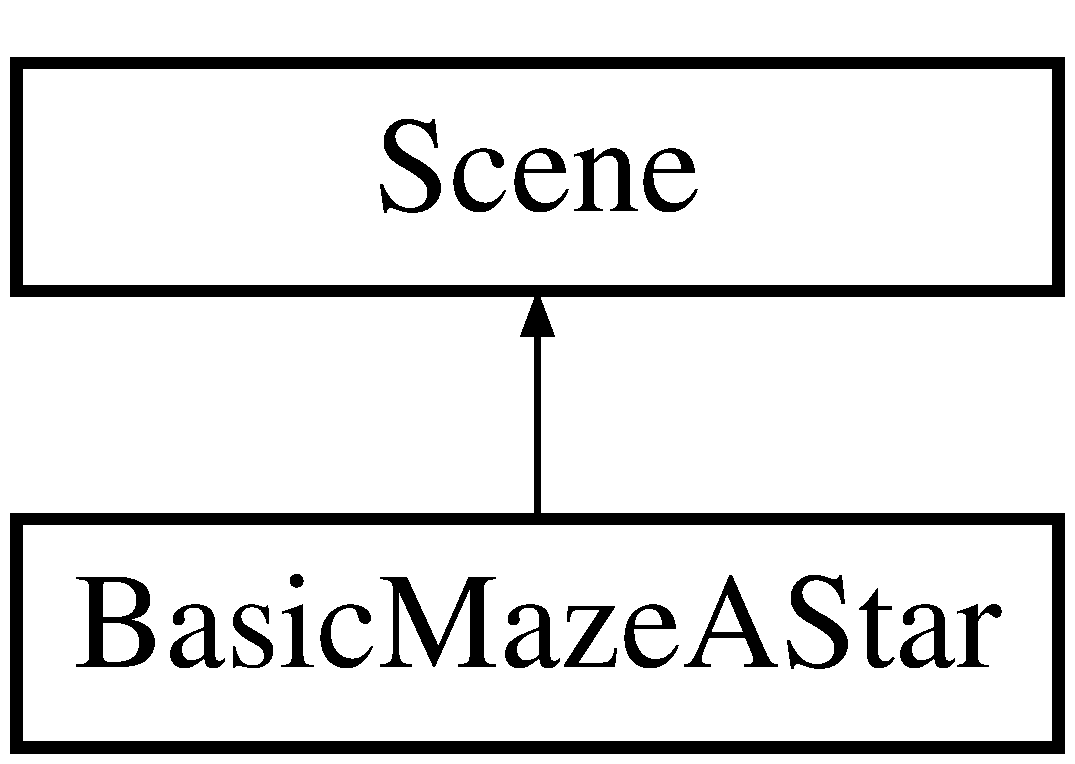
\includegraphics[height=2.000000cm]{class_basic_maze_a_star}
\end{center}
\end{figure}
\subsection*{Public Member Functions}
\begin{DoxyCompactItemize}
\item 
\hyperlink{class_basic_maze_a_star_a18afda3905b94b4a559bbb67324f5b5c}{Basic\-Maze\-A\-Star} (S\-D\-L\-\_\-\-Renderer $\ast$\-\_\-renderer)
\item 
\hyperlink{class_basic_maze_a_star_acaced8c2875e8544790f02d3e51aa25c}{$\sim$\-Basic\-Maze\-A\-Star} (void)
\item 
void \hyperlink{class_basic_maze_a_star_a4734bf9b21100b2dec42c44a0aa5421b}{Draw} ()
\item 
void \hyperlink{class_basic_maze_a_star_aca11eda868180204813e3e7ded4dbf81}{Update} ()
\end{DoxyCompactItemize}


\subsection{Constructor \& Destructor Documentation}
\hypertarget{class_basic_maze_a_star_a18afda3905b94b4a559bbb67324f5b5c}{\index{Basic\-Maze\-A\-Star@{Basic\-Maze\-A\-Star}!Basic\-Maze\-A\-Star@{Basic\-Maze\-A\-Star}}
\index{Basic\-Maze\-A\-Star@{Basic\-Maze\-A\-Star}!BasicMazeAStar@{Basic\-Maze\-A\-Star}}
\subsubsection[{Basic\-Maze\-A\-Star}]{\setlength{\rightskip}{0pt plus 5cm}Basic\-Maze\-A\-Star\-::\-Basic\-Maze\-A\-Star (
\begin{DoxyParamCaption}
\item[{S\-D\-L\-\_\-\-Renderer $\ast$}]{\-\_\-renderer}
\end{DoxyParamCaption}
)}}\label{class_basic_maze_a_star_a18afda3905b94b4a559bbb67324f5b5c}
\hypertarget{class_basic_maze_a_star_acaced8c2875e8544790f02d3e51aa25c}{\index{Basic\-Maze\-A\-Star@{Basic\-Maze\-A\-Star}!$\sim$\-Basic\-Maze\-A\-Star@{$\sim$\-Basic\-Maze\-A\-Star}}
\index{$\sim$\-Basic\-Maze\-A\-Star@{$\sim$\-Basic\-Maze\-A\-Star}!BasicMazeAStar@{Basic\-Maze\-A\-Star}}
\subsubsection[{$\sim$\-Basic\-Maze\-A\-Star}]{\setlength{\rightskip}{0pt plus 5cm}Basic\-Maze\-A\-Star\-::$\sim$\-Basic\-Maze\-A\-Star (
\begin{DoxyParamCaption}
\item[{void}]{}
\end{DoxyParamCaption}
)}}\label{class_basic_maze_a_star_acaced8c2875e8544790f02d3e51aa25c}


\subsection{Member Function Documentation}
\hypertarget{class_basic_maze_a_star_a4734bf9b21100b2dec42c44a0aa5421b}{\index{Basic\-Maze\-A\-Star@{Basic\-Maze\-A\-Star}!Draw@{Draw}}
\index{Draw@{Draw}!BasicMazeAStar@{Basic\-Maze\-A\-Star}}
\subsubsection[{Draw}]{\setlength{\rightskip}{0pt plus 5cm}void Basic\-Maze\-A\-Star\-::\-Draw (
\begin{DoxyParamCaption}
{}
\end{DoxyParamCaption}
)}}\label{class_basic_maze_a_star_a4734bf9b21100b2dec42c44a0aa5421b}
\hypertarget{class_basic_maze_a_star_aca11eda868180204813e3e7ded4dbf81}{\index{Basic\-Maze\-A\-Star@{Basic\-Maze\-A\-Star}!Update@{Update}}
\index{Update@{Update}!BasicMazeAStar@{Basic\-Maze\-A\-Star}}
\subsubsection[{Update}]{\setlength{\rightskip}{0pt plus 5cm}void Basic\-Maze\-A\-Star\-::\-Update (
\begin{DoxyParamCaption}
{}
\end{DoxyParamCaption}
)}}\label{class_basic_maze_a_star_aca11eda868180204813e3e7ded4dbf81}


The documentation for this class was generated from the following file\-:\begin{DoxyCompactItemize}
\item 
Joes\-\_\-\-S\-D\-L\-\_\-\-Framework/\hyperlink{_basic_maze_a_star_8h}{Basic\-Maze\-A\-Star.\-h}\end{DoxyCompactItemize}

\hypertarget{class_desert}{\section{Desert Class Reference}
\label{class_desert}\index{Desert@{Desert}}
}


{\ttfamily \#include $<$Desert.\-h$>$}

Inheritance diagram for Desert\-:\begin{figure}[H]
\begin{center}
\leavevmode
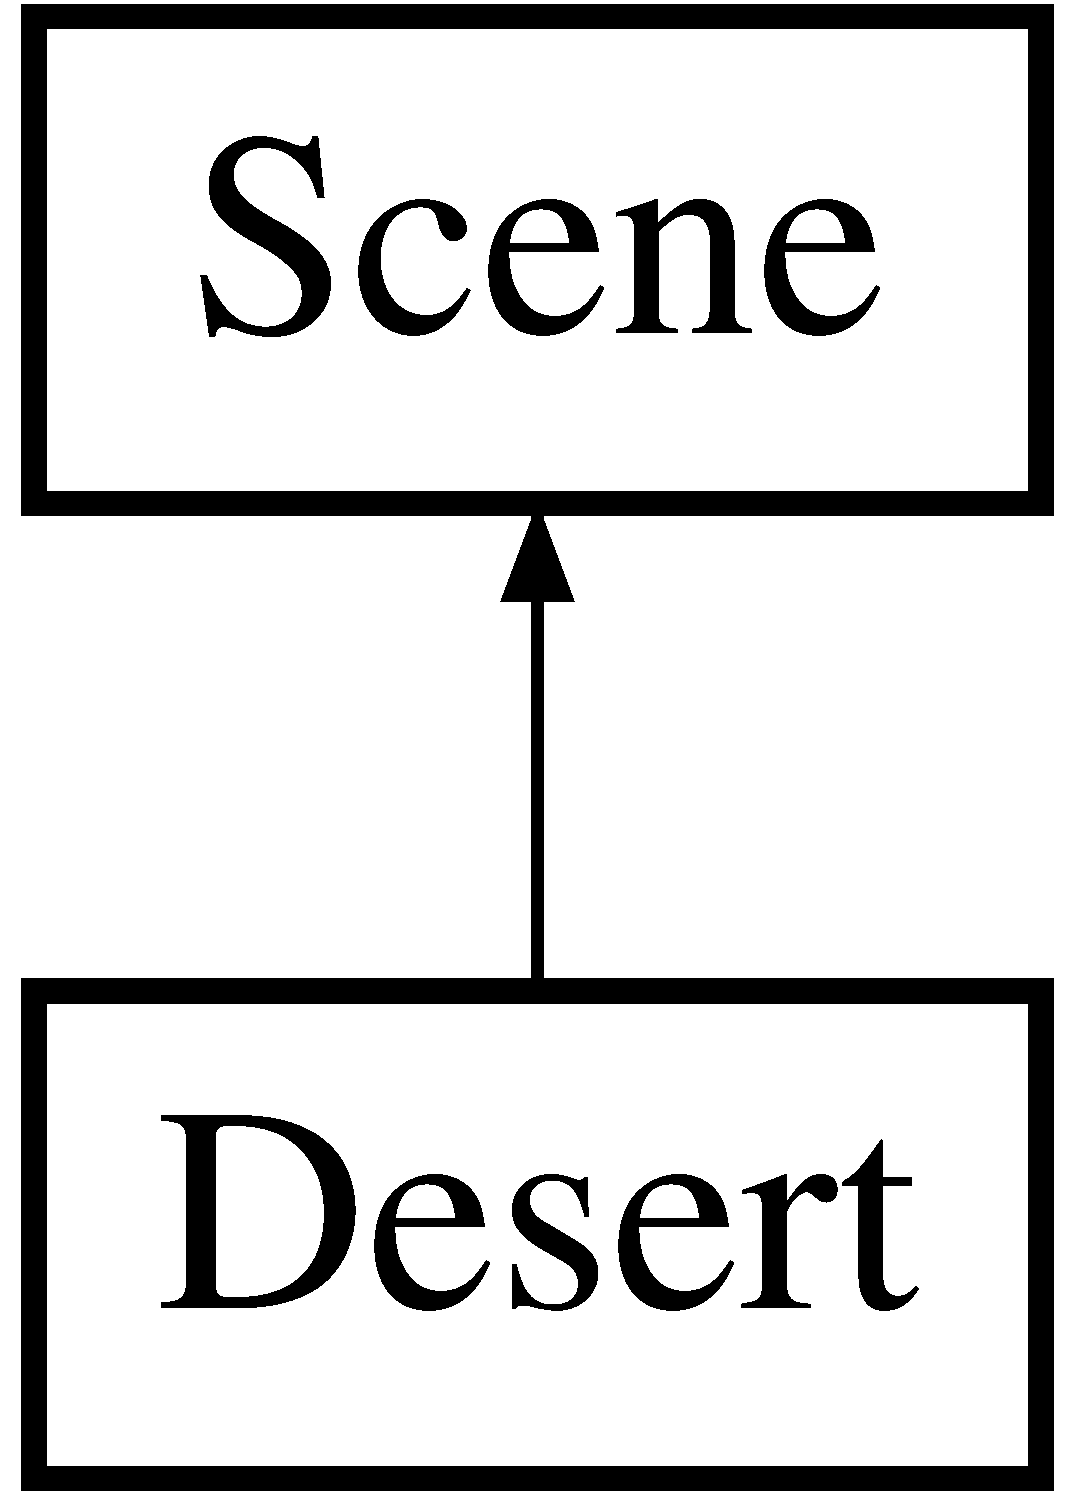
\includegraphics[height=2.000000cm]{class_desert}
\end{center}
\end{figure}
\subsection*{Public Member Functions}
\begin{DoxyCompactItemize}
\item 
\hyperlink{class_desert_acc7faf4817d9ba1ef97b5c5dd2198dce}{Desert} (S\-D\-L\-\_\-\-Renderer $\ast$\-\_\-renderer)
\item 
\hyperlink{class_desert_a9e1bcad506953f0580bb71bde96e64b6}{$\sim$\-Desert} (void)
\item 
void \hyperlink{class_desert_a43171056e9831ced675029ac7c26670b}{Draw} ()
\item 
void \hyperlink{class_desert_afba57b5245419e992bad9bf07107a5e8}{Update} ()
\end{DoxyCompactItemize}


\subsection{Constructor \& Destructor Documentation}
\hypertarget{class_desert_acc7faf4817d9ba1ef97b5c5dd2198dce}{\index{Desert@{Desert}!Desert@{Desert}}
\index{Desert@{Desert}!Desert@{Desert}}
\subsubsection[{Desert}]{\setlength{\rightskip}{0pt plus 5cm}Desert\-::\-Desert (
\begin{DoxyParamCaption}
\item[{S\-D\-L\-\_\-\-Renderer $\ast$}]{\-\_\-renderer}
\end{DoxyParamCaption}
)}}\label{class_desert_acc7faf4817d9ba1ef97b5c5dd2198dce}
\hypertarget{class_desert_a9e1bcad506953f0580bb71bde96e64b6}{\index{Desert@{Desert}!$\sim$\-Desert@{$\sim$\-Desert}}
\index{$\sim$\-Desert@{$\sim$\-Desert}!Desert@{Desert}}
\subsubsection[{$\sim$\-Desert}]{\setlength{\rightskip}{0pt plus 5cm}Desert\-::$\sim$\-Desert (
\begin{DoxyParamCaption}
\item[{void}]{}
\end{DoxyParamCaption}
)}}\label{class_desert_a9e1bcad506953f0580bb71bde96e64b6}


\subsection{Member Function Documentation}
\hypertarget{class_desert_a43171056e9831ced675029ac7c26670b}{\index{Desert@{Desert}!Draw@{Draw}}
\index{Draw@{Draw}!Desert@{Desert}}
\subsubsection[{Draw}]{\setlength{\rightskip}{0pt plus 5cm}void Desert\-::\-Draw (
\begin{DoxyParamCaption}
{}
\end{DoxyParamCaption}
)}}\label{class_desert_a43171056e9831ced675029ac7c26670b}
\hypertarget{class_desert_afba57b5245419e992bad9bf07107a5e8}{\index{Desert@{Desert}!Update@{Update}}
\index{Update@{Update}!Desert@{Desert}}
\subsubsection[{Update}]{\setlength{\rightskip}{0pt plus 5cm}void Desert\-::\-Update (
\begin{DoxyParamCaption}
{}
\end{DoxyParamCaption}
)}}\label{class_desert_afba57b5245419e992bad9bf07107a5e8}


The documentation for this class was generated from the following file\-:\begin{DoxyCompactItemize}
\item 
Joes\-\_\-\-S\-D\-L\-\_\-\-Framework/\hyperlink{_desert_8h}{Desert.\-h}\end{DoxyCompactItemize}

\hypertarget{classtinyxml2_1_1_dyn_array}{\section{tinyxml2\-:\-:Dyn\-Array$<$ T, I\-N\-I\-T $>$ Class Template Reference}
\label{classtinyxml2_1_1_dyn_array}\index{tinyxml2\-::\-Dyn\-Array$<$ T, I\-N\-I\-T $>$@{tinyxml2\-::\-Dyn\-Array$<$ T, I\-N\-I\-T $>$}}
}


{\ttfamily \#include $<$tinyxml2.\-h$>$}

\subsection*{Public Member Functions}
\begin{DoxyCompactItemize}
\item 
\hyperlink{classtinyxml2_1_1_dyn_array_af076df9203a7eda3f3501a0c84dbbb8a}{Dyn\-Array} ()
\item 
\hyperlink{classtinyxml2_1_1_dyn_array_ac7c2dc82db9010d09041ea6bfd921fdc}{$\sim$\-Dyn\-Array} ()
\item 
void \hyperlink{classtinyxml2_1_1_dyn_array_a498de53808ba0151fef54ea10bf51050}{Push} (T t)
\item 
T $\ast$ \hyperlink{classtinyxml2_1_1_dyn_array_aa3c360d40addc3b05121da9f60a01b4d}{Push\-Arr} (int count)
\item 
T \hyperlink{classtinyxml2_1_1_dyn_array_a2281e3342bc235bf391a67e362c75866}{Pop} ()
\item 
void \hyperlink{classtinyxml2_1_1_dyn_array_ab45c0836d8c0260a5b9eda7da80de71c}{Pop\-Arr} (int count)
\item 
bool \hyperlink{classtinyxml2_1_1_dyn_array_a080dc4dc68713964bb17745d4c833158}{Empty} () const 
\item 
T \& \hyperlink{classtinyxml2_1_1_dyn_array_a775a6ab4d41f0eb15bdd863d408dd58f}{operator\mbox{[}$\,$\mbox{]}} (int i)
\item 
const T \& \hyperlink{classtinyxml2_1_1_dyn_array_a1f4874c2608cbd68be1627fca9efd820}{operator\mbox{[}$\,$\mbox{]}} (int i) const 
\item 
const T \& \hyperlink{classtinyxml2_1_1_dyn_array_a9c2282ea8901b5a92ccaac2e6166a788}{Peek\-Top} () const 
\item 
int \hyperlink{classtinyxml2_1_1_dyn_array_a1299b257b62ea6b4983c488867f219b0}{Size} () const 
\item 
int \hyperlink{classtinyxml2_1_1_dyn_array_a8edbe90ed53b2e46b1b5cf53b261e4e7}{Capacity} () const 
\item 
const T $\ast$ \hyperlink{classtinyxml2_1_1_dyn_array_a1f39330daeb97d3d1dc3fc12dcf7ac67}{Mem} () const 
\item 
T $\ast$ \hyperlink{classtinyxml2_1_1_dyn_array_a0e0d60b399d54fad5b33d5008bc59c8e}{Mem} ()
\end{DoxyCompactItemize}


\subsection{Constructor \& Destructor Documentation}
\hypertarget{classtinyxml2_1_1_dyn_array_af076df9203a7eda3f3501a0c84dbbb8a}{\index{tinyxml2\-::\-Dyn\-Array@{tinyxml2\-::\-Dyn\-Array}!Dyn\-Array@{Dyn\-Array}}
\index{Dyn\-Array@{Dyn\-Array}!tinyxml2::DynArray@{tinyxml2\-::\-Dyn\-Array}}
\subsubsection[{Dyn\-Array}]{\setlength{\rightskip}{0pt plus 5cm}template$<$class T, int I\-N\-I\-T$>$ {\bf tinyxml2\-::\-Dyn\-Array}$<$ T, I\-N\-I\-T $>$\-::{\bf Dyn\-Array} (
\begin{DoxyParamCaption}
{}
\end{DoxyParamCaption}
)\hspace{0.3cm}{\ttfamily [inline]}}}\label{classtinyxml2_1_1_dyn_array_af076df9203a7eda3f3501a0c84dbbb8a}
\hypertarget{classtinyxml2_1_1_dyn_array_ac7c2dc82db9010d09041ea6bfd921fdc}{\index{tinyxml2\-::\-Dyn\-Array@{tinyxml2\-::\-Dyn\-Array}!$\sim$\-Dyn\-Array@{$\sim$\-Dyn\-Array}}
\index{$\sim$\-Dyn\-Array@{$\sim$\-Dyn\-Array}!tinyxml2::DynArray@{tinyxml2\-::\-Dyn\-Array}}
\subsubsection[{$\sim$\-Dyn\-Array}]{\setlength{\rightskip}{0pt plus 5cm}template$<$class T, int I\-N\-I\-T$>$ {\bf tinyxml2\-::\-Dyn\-Array}$<$ T, I\-N\-I\-T $>$\-::$\sim${\bf Dyn\-Array} (
\begin{DoxyParamCaption}
{}
\end{DoxyParamCaption}
)\hspace{0.3cm}{\ttfamily [inline]}}}\label{classtinyxml2_1_1_dyn_array_ac7c2dc82db9010d09041ea6bfd921fdc}


\subsection{Member Function Documentation}
\hypertarget{classtinyxml2_1_1_dyn_array_a8edbe90ed53b2e46b1b5cf53b261e4e7}{\index{tinyxml2\-::\-Dyn\-Array@{tinyxml2\-::\-Dyn\-Array}!Capacity@{Capacity}}
\index{Capacity@{Capacity}!tinyxml2::DynArray@{tinyxml2\-::\-Dyn\-Array}}
\subsubsection[{Capacity}]{\setlength{\rightskip}{0pt plus 5cm}template$<$class T, int I\-N\-I\-T$>$ int {\bf tinyxml2\-::\-Dyn\-Array}$<$ T, I\-N\-I\-T $>$\-::Capacity (
\begin{DoxyParamCaption}
{}
\end{DoxyParamCaption}
) const\hspace{0.3cm}{\ttfamily [inline]}}}\label{classtinyxml2_1_1_dyn_array_a8edbe90ed53b2e46b1b5cf53b261e4e7}
\hypertarget{classtinyxml2_1_1_dyn_array_a080dc4dc68713964bb17745d4c833158}{\index{tinyxml2\-::\-Dyn\-Array@{tinyxml2\-::\-Dyn\-Array}!Empty@{Empty}}
\index{Empty@{Empty}!tinyxml2::DynArray@{tinyxml2\-::\-Dyn\-Array}}
\subsubsection[{Empty}]{\setlength{\rightskip}{0pt plus 5cm}template$<$class T, int I\-N\-I\-T$>$ bool {\bf tinyxml2\-::\-Dyn\-Array}$<$ T, I\-N\-I\-T $>$\-::Empty (
\begin{DoxyParamCaption}
{}
\end{DoxyParamCaption}
) const\hspace{0.3cm}{\ttfamily [inline]}}}\label{classtinyxml2_1_1_dyn_array_a080dc4dc68713964bb17745d4c833158}
\hypertarget{classtinyxml2_1_1_dyn_array_a1f39330daeb97d3d1dc3fc12dcf7ac67}{\index{tinyxml2\-::\-Dyn\-Array@{tinyxml2\-::\-Dyn\-Array}!Mem@{Mem}}
\index{Mem@{Mem}!tinyxml2::DynArray@{tinyxml2\-::\-Dyn\-Array}}
\subsubsection[{Mem}]{\setlength{\rightskip}{0pt plus 5cm}template$<$class T, int I\-N\-I\-T$>$ const T$\ast$ {\bf tinyxml2\-::\-Dyn\-Array}$<$ T, I\-N\-I\-T $>$\-::Mem (
\begin{DoxyParamCaption}
{}
\end{DoxyParamCaption}
) const\hspace{0.3cm}{\ttfamily [inline]}}}\label{classtinyxml2_1_1_dyn_array_a1f39330daeb97d3d1dc3fc12dcf7ac67}
\hypertarget{classtinyxml2_1_1_dyn_array_a0e0d60b399d54fad5b33d5008bc59c8e}{\index{tinyxml2\-::\-Dyn\-Array@{tinyxml2\-::\-Dyn\-Array}!Mem@{Mem}}
\index{Mem@{Mem}!tinyxml2::DynArray@{tinyxml2\-::\-Dyn\-Array}}
\subsubsection[{Mem}]{\setlength{\rightskip}{0pt plus 5cm}template$<$class T, int I\-N\-I\-T$>$ T$\ast$ {\bf tinyxml2\-::\-Dyn\-Array}$<$ T, I\-N\-I\-T $>$\-::Mem (
\begin{DoxyParamCaption}
{}
\end{DoxyParamCaption}
)\hspace{0.3cm}{\ttfamily [inline]}}}\label{classtinyxml2_1_1_dyn_array_a0e0d60b399d54fad5b33d5008bc59c8e}
\hypertarget{classtinyxml2_1_1_dyn_array_a775a6ab4d41f0eb15bdd863d408dd58f}{\index{tinyxml2\-::\-Dyn\-Array@{tinyxml2\-::\-Dyn\-Array}!operator\mbox{[}$\,$\mbox{]}@{operator[]}}
\index{operator\mbox{[}$\,$\mbox{]}@{operator[]}!tinyxml2::DynArray@{tinyxml2\-::\-Dyn\-Array}}
\subsubsection[{operator[]}]{\setlength{\rightskip}{0pt plus 5cm}template$<$class T, int I\-N\-I\-T$>$ T\& {\bf tinyxml2\-::\-Dyn\-Array}$<$ T, I\-N\-I\-T $>$\-::operator\mbox{[}$\,$\mbox{]} (
\begin{DoxyParamCaption}
\item[{int}]{i}
\end{DoxyParamCaption}
)\hspace{0.3cm}{\ttfamily [inline]}}}\label{classtinyxml2_1_1_dyn_array_a775a6ab4d41f0eb15bdd863d408dd58f}
\hypertarget{classtinyxml2_1_1_dyn_array_a1f4874c2608cbd68be1627fca9efd820}{\index{tinyxml2\-::\-Dyn\-Array@{tinyxml2\-::\-Dyn\-Array}!operator\mbox{[}$\,$\mbox{]}@{operator[]}}
\index{operator\mbox{[}$\,$\mbox{]}@{operator[]}!tinyxml2::DynArray@{tinyxml2\-::\-Dyn\-Array}}
\subsubsection[{operator[]}]{\setlength{\rightskip}{0pt plus 5cm}template$<$class T, int I\-N\-I\-T$>$ const T\& {\bf tinyxml2\-::\-Dyn\-Array}$<$ T, I\-N\-I\-T $>$\-::operator\mbox{[}$\,$\mbox{]} (
\begin{DoxyParamCaption}
\item[{int}]{i}
\end{DoxyParamCaption}
) const\hspace{0.3cm}{\ttfamily [inline]}}}\label{classtinyxml2_1_1_dyn_array_a1f4874c2608cbd68be1627fca9efd820}
\hypertarget{classtinyxml2_1_1_dyn_array_a9c2282ea8901b5a92ccaac2e6166a788}{\index{tinyxml2\-::\-Dyn\-Array@{tinyxml2\-::\-Dyn\-Array}!Peek\-Top@{Peek\-Top}}
\index{Peek\-Top@{Peek\-Top}!tinyxml2::DynArray@{tinyxml2\-::\-Dyn\-Array}}
\subsubsection[{Peek\-Top}]{\setlength{\rightskip}{0pt plus 5cm}template$<$class T, int I\-N\-I\-T$>$ const T\& {\bf tinyxml2\-::\-Dyn\-Array}$<$ T, I\-N\-I\-T $>$\-::Peek\-Top (
\begin{DoxyParamCaption}
{}
\end{DoxyParamCaption}
) const\hspace{0.3cm}{\ttfamily [inline]}}}\label{classtinyxml2_1_1_dyn_array_a9c2282ea8901b5a92ccaac2e6166a788}
\hypertarget{classtinyxml2_1_1_dyn_array_a2281e3342bc235bf391a67e362c75866}{\index{tinyxml2\-::\-Dyn\-Array@{tinyxml2\-::\-Dyn\-Array}!Pop@{Pop}}
\index{Pop@{Pop}!tinyxml2::DynArray@{tinyxml2\-::\-Dyn\-Array}}
\subsubsection[{Pop}]{\setlength{\rightskip}{0pt plus 5cm}template$<$class T, int I\-N\-I\-T$>$ T {\bf tinyxml2\-::\-Dyn\-Array}$<$ T, I\-N\-I\-T $>$\-::Pop (
\begin{DoxyParamCaption}
{}
\end{DoxyParamCaption}
)\hspace{0.3cm}{\ttfamily [inline]}}}\label{classtinyxml2_1_1_dyn_array_a2281e3342bc235bf391a67e362c75866}
\hypertarget{classtinyxml2_1_1_dyn_array_ab45c0836d8c0260a5b9eda7da80de71c}{\index{tinyxml2\-::\-Dyn\-Array@{tinyxml2\-::\-Dyn\-Array}!Pop\-Arr@{Pop\-Arr}}
\index{Pop\-Arr@{Pop\-Arr}!tinyxml2::DynArray@{tinyxml2\-::\-Dyn\-Array}}
\subsubsection[{Pop\-Arr}]{\setlength{\rightskip}{0pt plus 5cm}template$<$class T, int I\-N\-I\-T$>$ void {\bf tinyxml2\-::\-Dyn\-Array}$<$ T, I\-N\-I\-T $>$\-::Pop\-Arr (
\begin{DoxyParamCaption}
\item[{int}]{count}
\end{DoxyParamCaption}
)\hspace{0.3cm}{\ttfamily [inline]}}}\label{classtinyxml2_1_1_dyn_array_ab45c0836d8c0260a5b9eda7da80de71c}
\hypertarget{classtinyxml2_1_1_dyn_array_a498de53808ba0151fef54ea10bf51050}{\index{tinyxml2\-::\-Dyn\-Array@{tinyxml2\-::\-Dyn\-Array}!Push@{Push}}
\index{Push@{Push}!tinyxml2::DynArray@{tinyxml2\-::\-Dyn\-Array}}
\subsubsection[{Push}]{\setlength{\rightskip}{0pt plus 5cm}template$<$class T, int I\-N\-I\-T$>$ void {\bf tinyxml2\-::\-Dyn\-Array}$<$ T, I\-N\-I\-T $>$\-::Push (
\begin{DoxyParamCaption}
\item[{T}]{t}
\end{DoxyParamCaption}
)\hspace{0.3cm}{\ttfamily [inline]}}}\label{classtinyxml2_1_1_dyn_array_a498de53808ba0151fef54ea10bf51050}
\hypertarget{classtinyxml2_1_1_dyn_array_aa3c360d40addc3b05121da9f60a01b4d}{\index{tinyxml2\-::\-Dyn\-Array@{tinyxml2\-::\-Dyn\-Array}!Push\-Arr@{Push\-Arr}}
\index{Push\-Arr@{Push\-Arr}!tinyxml2::DynArray@{tinyxml2\-::\-Dyn\-Array}}
\subsubsection[{Push\-Arr}]{\setlength{\rightskip}{0pt plus 5cm}template$<$class T, int I\-N\-I\-T$>$ T$\ast$ {\bf tinyxml2\-::\-Dyn\-Array}$<$ T, I\-N\-I\-T $>$\-::Push\-Arr (
\begin{DoxyParamCaption}
\item[{int}]{count}
\end{DoxyParamCaption}
)\hspace{0.3cm}{\ttfamily [inline]}}}\label{classtinyxml2_1_1_dyn_array_aa3c360d40addc3b05121da9f60a01b4d}
\hypertarget{classtinyxml2_1_1_dyn_array_a1299b257b62ea6b4983c488867f219b0}{\index{tinyxml2\-::\-Dyn\-Array@{tinyxml2\-::\-Dyn\-Array}!Size@{Size}}
\index{Size@{Size}!tinyxml2::DynArray@{tinyxml2\-::\-Dyn\-Array}}
\subsubsection[{Size}]{\setlength{\rightskip}{0pt plus 5cm}template$<$class T, int I\-N\-I\-T$>$ int {\bf tinyxml2\-::\-Dyn\-Array}$<$ T, I\-N\-I\-T $>$\-::Size (
\begin{DoxyParamCaption}
{}
\end{DoxyParamCaption}
) const\hspace{0.3cm}{\ttfamily [inline]}}}\label{classtinyxml2_1_1_dyn_array_a1299b257b62ea6b4983c488867f219b0}


The documentation for this class was generated from the following file\-:\begin{DoxyCompactItemize}
\item 
Joes\-\_\-\-S\-D\-L\-\_\-\-Framework/\hyperlink{tinyxml2_8h}{tinyxml2.\-h}\end{DoxyCompactItemize}

\hypertarget{structtinyxml2_1_1_entity}{\section{tinyxml2\-:\-:Entity Struct Reference}
\label{structtinyxml2_1_1_entity}\index{tinyxml2\-::\-Entity@{tinyxml2\-::\-Entity}}
}
\subsection*{Public Attributes}
\begin{DoxyCompactItemize}
\item 
const char $\ast$ \hyperlink{structtinyxml2_1_1_entity_ab330f5d665d29bfc811ecfa76315894b}{pattern}
\item 
int \hyperlink{structtinyxml2_1_1_entity_a25e2b57cb59cb4fa68f283d7cb570f21}{length}
\item 
char \hyperlink{structtinyxml2_1_1_entity_a7334e81e33b4615655a403711b24f3ed}{value}
\end{DoxyCompactItemize}


\subsection{Member Data Documentation}
\hypertarget{structtinyxml2_1_1_entity_a25e2b57cb59cb4fa68f283d7cb570f21}{\index{tinyxml2\-::\-Entity@{tinyxml2\-::\-Entity}!length@{length}}
\index{length@{length}!tinyxml2::Entity@{tinyxml2\-::\-Entity}}
\subsubsection[{length}]{\setlength{\rightskip}{0pt plus 5cm}int tinyxml2\-::\-Entity\-::length}}\label{structtinyxml2_1_1_entity_a25e2b57cb59cb4fa68f283d7cb570f21}
\hypertarget{structtinyxml2_1_1_entity_ab330f5d665d29bfc811ecfa76315894b}{\index{tinyxml2\-::\-Entity@{tinyxml2\-::\-Entity}!pattern@{pattern}}
\index{pattern@{pattern}!tinyxml2::Entity@{tinyxml2\-::\-Entity}}
\subsubsection[{pattern}]{\setlength{\rightskip}{0pt plus 5cm}const char$\ast$ tinyxml2\-::\-Entity\-::pattern}}\label{structtinyxml2_1_1_entity_ab330f5d665d29bfc811ecfa76315894b}
\hypertarget{structtinyxml2_1_1_entity_a7334e81e33b4615655a403711b24f3ed}{\index{tinyxml2\-::\-Entity@{tinyxml2\-::\-Entity}!value@{value}}
\index{value@{value}!tinyxml2::Entity@{tinyxml2\-::\-Entity}}
\subsubsection[{value}]{\setlength{\rightskip}{0pt plus 5cm}char tinyxml2\-::\-Entity\-::value}}\label{structtinyxml2_1_1_entity_a7334e81e33b4615655a403711b24f3ed}


The documentation for this struct was generated from the following file\-:\begin{DoxyCompactItemize}
\item 
Joes\-\_\-\-S\-D\-L\-\_\-\-Framework/\hyperlink{tinyxml2_8cpp}{tinyxml2.\-cpp}\end{DoxyCompactItemize}

\hypertarget{class_iso_layer}{\section{Iso\-Layer Class Reference}
\label{class_iso_layer}\index{Iso\-Layer@{Iso\-Layer}}
}


{\ttfamily \#include $<$Iso\-Layer.\-h$>$}

\subsection*{Public Member Functions}
\begin{DoxyCompactItemize}
\item 
\hyperlink{class_iso_layer_a37dab3b9120d6ffce8a9e7ee61ddba00}{Iso\-Layer} (\hyperlink{classtinyxml2_1_1_x_m_l_element}{X\-M\-L\-Element} $\ast$\-\_\-layer, int \-\_\-tiles\-Num\-Width, int \-\_\-tiles\-Num\-Height, int \-\_\-tile\-Sheet\-Width, char $\ast$\-\_\-name\-Of\-Sprite\-Sheet, int \-\_\-tiles\-Width, int \-\_\-tiles\-Height, S\-D\-L\-\_\-\-Renderer $\ast$\-\_\-renderer, int \-\_\-spacing, int \-\_\-margin, int \-\_\-gid\-Fixer)
\item 
\hyperlink{class_iso_layer_a5fe18022f5cf3cd49718fa52a0a239ba}{$\sim$\-Iso\-Layer} (void)
\item 
void \hyperlink{class_iso_layer_a10856b4ee71ec47c70bdb88ba99f3577}{Update} ()
\item 
void \hyperlink{class_iso_layer_afb67093891aaf8185de5ce1f5c9fb4b7}{Draw} ()
\end{DoxyCompactItemize}
\subsection*{Public Attributes}
\begin{DoxyCompactItemize}
\item 
vector$<$ \hyperlink{class_x_d_l___sprite}{X\-D\-L\-\_\-\-Sprite} $\ast$ $>$ \hyperlink{class_iso_layer_a4174fb6589bb484bb97f670665e56172}{\-\_\-tiles}
\end{DoxyCompactItemize}


\subsection{Constructor \& Destructor Documentation}
\hypertarget{class_iso_layer_a37dab3b9120d6ffce8a9e7ee61ddba00}{\index{Iso\-Layer@{Iso\-Layer}!Iso\-Layer@{Iso\-Layer}}
\index{Iso\-Layer@{Iso\-Layer}!IsoLayer@{Iso\-Layer}}
\subsubsection[{Iso\-Layer}]{\setlength{\rightskip}{0pt plus 5cm}Iso\-Layer\-::\-Iso\-Layer (
\begin{DoxyParamCaption}
\item[{{\bf X\-M\-L\-Element} $\ast$}]{\-\_\-layer, }
\item[{int}]{\-\_\-tiles\-Num\-Width, }
\item[{int}]{\-\_\-tiles\-Num\-Height, }
\item[{int}]{\-\_\-tile\-Sheet\-Width, }
\item[{char $\ast$}]{\-\_\-name\-Of\-Sprite\-Sheet, }
\item[{int}]{\-\_\-tiles\-Width, }
\item[{int}]{\-\_\-tiles\-Height, }
\item[{S\-D\-L\-\_\-\-Renderer $\ast$}]{\-\_\-renderer, }
\item[{int}]{\-\_\-spacing, }
\item[{int}]{\-\_\-margin, }
\item[{int}]{\-\_\-gid\-Fixer}
\end{DoxyParamCaption}
)}}\label{class_iso_layer_a37dab3b9120d6ffce8a9e7ee61ddba00}
\hypertarget{class_iso_layer_a5fe18022f5cf3cd49718fa52a0a239ba}{\index{Iso\-Layer@{Iso\-Layer}!$\sim$\-Iso\-Layer@{$\sim$\-Iso\-Layer}}
\index{$\sim$\-Iso\-Layer@{$\sim$\-Iso\-Layer}!IsoLayer@{Iso\-Layer}}
\subsubsection[{$\sim$\-Iso\-Layer}]{\setlength{\rightskip}{0pt plus 5cm}Iso\-Layer\-::$\sim$\-Iso\-Layer (
\begin{DoxyParamCaption}
\item[{void}]{}
\end{DoxyParamCaption}
)}}\label{class_iso_layer_a5fe18022f5cf3cd49718fa52a0a239ba}


\subsection{Member Function Documentation}
\hypertarget{class_iso_layer_afb67093891aaf8185de5ce1f5c9fb4b7}{\index{Iso\-Layer@{Iso\-Layer}!Draw@{Draw}}
\index{Draw@{Draw}!IsoLayer@{Iso\-Layer}}
\subsubsection[{Draw}]{\setlength{\rightskip}{0pt plus 5cm}void Iso\-Layer\-::\-Draw (
\begin{DoxyParamCaption}
{}
\end{DoxyParamCaption}
)}}\label{class_iso_layer_afb67093891aaf8185de5ce1f5c9fb4b7}
\hypertarget{class_iso_layer_a10856b4ee71ec47c70bdb88ba99f3577}{\index{Iso\-Layer@{Iso\-Layer}!Update@{Update}}
\index{Update@{Update}!IsoLayer@{Iso\-Layer}}
\subsubsection[{Update}]{\setlength{\rightskip}{0pt plus 5cm}void Iso\-Layer\-::\-Update (
\begin{DoxyParamCaption}
{}
\end{DoxyParamCaption}
)}}\label{class_iso_layer_a10856b4ee71ec47c70bdb88ba99f3577}


\subsection{Member Data Documentation}
\hypertarget{class_iso_layer_a4174fb6589bb484bb97f670665e56172}{\index{Iso\-Layer@{Iso\-Layer}!\-\_\-tiles@{\-\_\-tiles}}
\index{\-\_\-tiles@{\-\_\-tiles}!IsoLayer@{Iso\-Layer}}
\subsubsection[{\-\_\-tiles}]{\setlength{\rightskip}{0pt plus 5cm}vector$<${\bf X\-D\-L\-\_\-\-Sprite}$\ast$$>$ Iso\-Layer\-::\-\_\-tiles}}\label{class_iso_layer_a4174fb6589bb484bb97f670665e56172}


The documentation for this class was generated from the following files\-:\begin{DoxyCompactItemize}
\item 
Joes\-\_\-\-S\-D\-L\-\_\-\-Framework/\hyperlink{_iso_layer_8h}{Iso\-Layer.\-h}\item 
Joes\-\_\-\-S\-D\-L\-\_\-\-Framework/\hyperlink{_iso_layer_8cpp}{Iso\-Layer.\-cpp}\end{DoxyCompactItemize}

\hypertarget{class_isometric_tile_engine}{\section{Isometric\-Tile\-Engine Class Reference}
\label{class_isometric_tile_engine}\index{Isometric\-Tile\-Engine@{Isometric\-Tile\-Engine}}
}


{\ttfamily \#include $<$Isometric\-Tile\-Engine.\-h$>$}

\subsection*{Public Member Functions}
\begin{DoxyCompactItemize}
\item 
\hyperlink{class_isometric_tile_engine_af9a766bfe8514a4d2554d6d574cd7a1d}{Isometric\-Tile\-Engine} (S\-D\-L\-\_\-\-Renderer $\ast$\-\_\-renderer, int \-\_\-tiles\-Width, int \-\_\-tiles\-Height)
\item 
\hyperlink{class_isometric_tile_engine_a279b6dc6e3baa6f3dac19d7e6c7740e3}{$\sim$\-Isometric\-Tile\-Engine} (void)
\item 
void \hyperlink{class_isometric_tile_engine_a4c163c820bfc4b3fba05a0127f030cc0}{Update} ()
\item 
void \hyperlink{class_isometric_tile_engine_ad1da980ee1b9972dd05b51167fa32573}{Draw} ()
\item 
bool \hyperlink{class_isometric_tile_engine_ac0da404c4c4a4129c6da8eeb66bf3f32}{Load\-From\-X\-M\-L} (char $\ast$\-\_\-path\-To\-T\-M\-X)
\end{DoxyCompactItemize}


\subsection{Constructor \& Destructor Documentation}
\hypertarget{class_isometric_tile_engine_af9a766bfe8514a4d2554d6d574cd7a1d}{\index{Isometric\-Tile\-Engine@{Isometric\-Tile\-Engine}!Isometric\-Tile\-Engine@{Isometric\-Tile\-Engine}}
\index{Isometric\-Tile\-Engine@{Isometric\-Tile\-Engine}!IsometricTileEngine@{Isometric\-Tile\-Engine}}
\subsubsection[{Isometric\-Tile\-Engine}]{\setlength{\rightskip}{0pt plus 5cm}Isometric\-Tile\-Engine\-::\-Isometric\-Tile\-Engine (
\begin{DoxyParamCaption}
\item[{S\-D\-L\-\_\-\-Renderer $\ast$}]{\-\_\-renderer, }
\item[{int}]{\-\_\-tiles\-Width, }
\item[{int}]{\-\_\-tiles\-Height}
\end{DoxyParamCaption}
)}}\label{class_isometric_tile_engine_af9a766bfe8514a4d2554d6d574cd7a1d}
\hypertarget{class_isometric_tile_engine_a279b6dc6e3baa6f3dac19d7e6c7740e3}{\index{Isometric\-Tile\-Engine@{Isometric\-Tile\-Engine}!$\sim$\-Isometric\-Tile\-Engine@{$\sim$\-Isometric\-Tile\-Engine}}
\index{$\sim$\-Isometric\-Tile\-Engine@{$\sim$\-Isometric\-Tile\-Engine}!IsometricTileEngine@{Isometric\-Tile\-Engine}}
\subsubsection[{$\sim$\-Isometric\-Tile\-Engine}]{\setlength{\rightskip}{0pt plus 5cm}Isometric\-Tile\-Engine\-::$\sim$\-Isometric\-Tile\-Engine (
\begin{DoxyParamCaption}
\item[{void}]{}
\end{DoxyParamCaption}
)}}\label{class_isometric_tile_engine_a279b6dc6e3baa6f3dac19d7e6c7740e3}


\subsection{Member Function Documentation}
\hypertarget{class_isometric_tile_engine_ad1da980ee1b9972dd05b51167fa32573}{\index{Isometric\-Tile\-Engine@{Isometric\-Tile\-Engine}!Draw@{Draw}}
\index{Draw@{Draw}!IsometricTileEngine@{Isometric\-Tile\-Engine}}
\subsubsection[{Draw}]{\setlength{\rightskip}{0pt plus 5cm}void Isometric\-Tile\-Engine\-::\-Draw (
\begin{DoxyParamCaption}
{}
\end{DoxyParamCaption}
)}}\label{class_isometric_tile_engine_ad1da980ee1b9972dd05b51167fa32573}
\hypertarget{class_isometric_tile_engine_ac0da404c4c4a4129c6da8eeb66bf3f32}{\index{Isometric\-Tile\-Engine@{Isometric\-Tile\-Engine}!Load\-From\-X\-M\-L@{Load\-From\-X\-M\-L}}
\index{Load\-From\-X\-M\-L@{Load\-From\-X\-M\-L}!IsometricTileEngine@{Isometric\-Tile\-Engine}}
\subsubsection[{Load\-From\-X\-M\-L}]{\setlength{\rightskip}{0pt plus 5cm}bool Isometric\-Tile\-Engine\-::\-Load\-From\-X\-M\-L (
\begin{DoxyParamCaption}
\item[{char $\ast$}]{\-\_\-path\-To\-T\-M\-X}
\end{DoxyParamCaption}
)}}\label{class_isometric_tile_engine_ac0da404c4c4a4129c6da8eeb66bf3f32}
\hypertarget{class_isometric_tile_engine_a4c163c820bfc4b3fba05a0127f030cc0}{\index{Isometric\-Tile\-Engine@{Isometric\-Tile\-Engine}!Update@{Update}}
\index{Update@{Update}!IsometricTileEngine@{Isometric\-Tile\-Engine}}
\subsubsection[{Update}]{\setlength{\rightskip}{0pt plus 5cm}void Isometric\-Tile\-Engine\-::\-Update (
\begin{DoxyParamCaption}
{}
\end{DoxyParamCaption}
)}}\label{class_isometric_tile_engine_a4c163c820bfc4b3fba05a0127f030cc0}


The documentation for this class was generated from the following files\-:\begin{DoxyCompactItemize}
\item 
Joes\-\_\-\-S\-D\-L\-\_\-\-Framework/\hyperlink{_isometric_tile_engine_8h}{Isometric\-Tile\-Engine.\-h}\item 
Joes\-\_\-\-S\-D\-L\-\_\-\-Framework/\hyperlink{_isometric_tile_engine_8cpp}{Isometric\-Tile\-Engine.\-cpp}\end{DoxyCompactItemize}

\hypertarget{class_level1}{\section{Level1 Class Reference}
\label{class_level1}\index{Level1@{Level1}}
}


{\ttfamily \#include $<$Level1.\-h$>$}

Inheritance diagram for Level1\-:\begin{figure}[H]
\begin{center}
\leavevmode
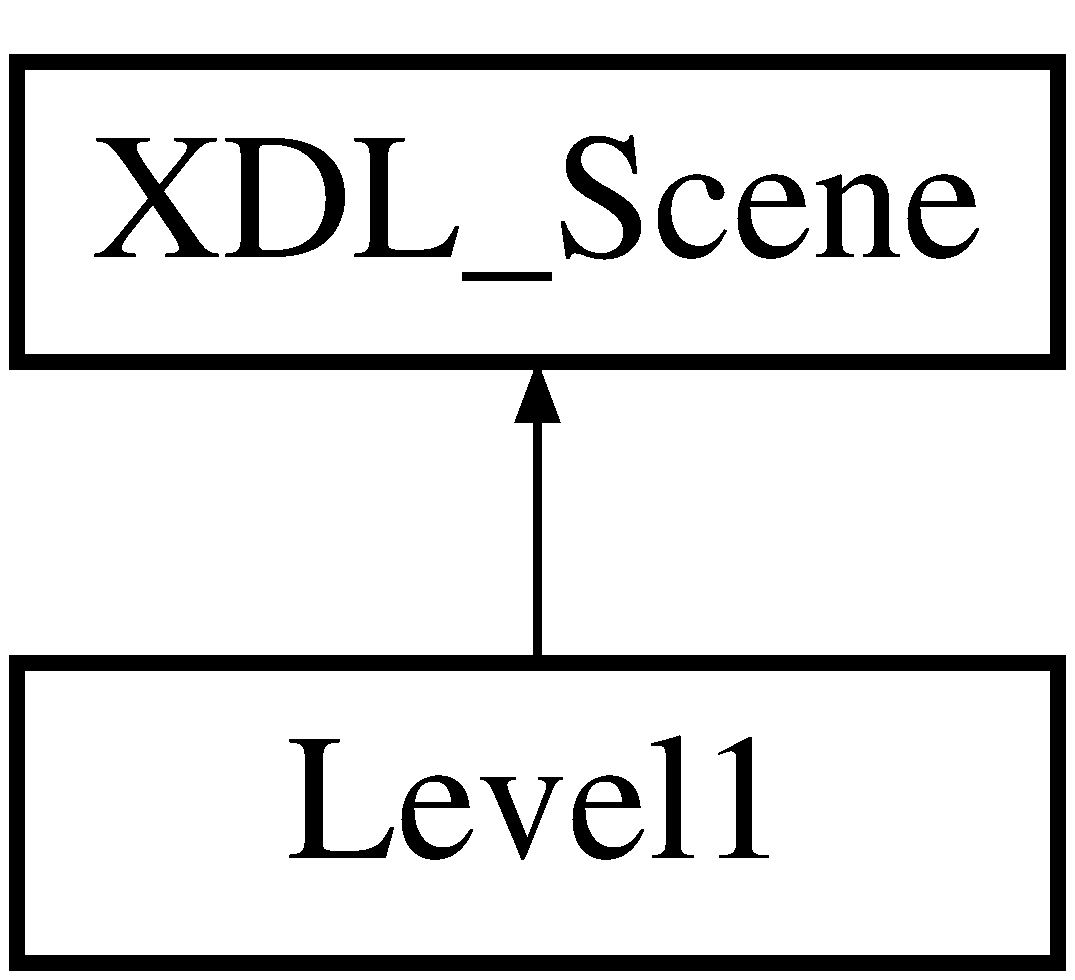
\includegraphics[height=2.000000cm]{class_level1}
\end{center}
\end{figure}
\subsection*{Public Member Functions}
\begin{DoxyCompactItemize}
\item 
\hyperlink{class_level1_a9fb42cfe27f4d15b86df761c556ad17a}{Level1} (S\-D\-L\-\_\-\-Renderer $\ast$\hyperlink{class_x_d_l___scene_a923ee55d91647c14f2566f1aa70e3aed}{\-\_\-renderer})
\item 
\hyperlink{class_level1_a8334c4e5a3070595d96b01e381b043fa}{$\sim$\-Level1} (void)
\item 
void \hyperlink{class_level1_ae8e845511c6fcf574f4f94cd0f986751}{Draw} ()
\item 
void \hyperlink{class_level1_a26cbf7e692665c1a1250162057583ee4}{Update} ()
\end{DoxyCompactItemize}
\subsection*{Additional Inherited Members}


\subsection{Constructor \& Destructor Documentation}
\hypertarget{class_level1_a9fb42cfe27f4d15b86df761c556ad17a}{\index{Level1@{Level1}!Level1@{Level1}}
\index{Level1@{Level1}!Level1@{Level1}}
\subsubsection[{Level1}]{\setlength{\rightskip}{0pt plus 5cm}Level1\-::\-Level1 (
\begin{DoxyParamCaption}
\item[{S\-D\-L\-\_\-\-Renderer $\ast$}]{\-\_\-renderer}
\end{DoxyParamCaption}
)}}\label{class_level1_a9fb42cfe27f4d15b86df761c556ad17a}
\hypertarget{class_level1_a8334c4e5a3070595d96b01e381b043fa}{\index{Level1@{Level1}!$\sim$\-Level1@{$\sim$\-Level1}}
\index{$\sim$\-Level1@{$\sim$\-Level1}!Level1@{Level1}}
\subsubsection[{$\sim$\-Level1}]{\setlength{\rightskip}{0pt plus 5cm}Level1\-::$\sim$\-Level1 (
\begin{DoxyParamCaption}
\item[{void}]{}
\end{DoxyParamCaption}
)}}\label{class_level1_a8334c4e5a3070595d96b01e381b043fa}


\subsection{Member Function Documentation}
\hypertarget{class_level1_ae8e845511c6fcf574f4f94cd0f986751}{\index{Level1@{Level1}!Draw@{Draw}}
\index{Draw@{Draw}!Level1@{Level1}}
\subsubsection[{Draw}]{\setlength{\rightskip}{0pt plus 5cm}void Level1\-::\-Draw (
\begin{DoxyParamCaption}
{}
\end{DoxyParamCaption}
)\hspace{0.3cm}{\ttfamily [virtual]}}}\label{class_level1_ae8e845511c6fcf574f4f94cd0f986751}


Reimplemented from \hyperlink{class_x_d_l___scene_a1a3d1b1f6a4f1f4c0834cc1fe29af814}{X\-D\-L\-\_\-\-Scene}.

\hypertarget{class_level1_a26cbf7e692665c1a1250162057583ee4}{\index{Level1@{Level1}!Update@{Update}}
\index{Update@{Update}!Level1@{Level1}}
\subsubsection[{Update}]{\setlength{\rightskip}{0pt plus 5cm}void Level1\-::\-Update (
\begin{DoxyParamCaption}
{}
\end{DoxyParamCaption}
)\hspace{0.3cm}{\ttfamily [virtual]}}}\label{class_level1_a26cbf7e692665c1a1250162057583ee4}


Reimplemented from \hyperlink{class_x_d_l___scene_abd1ce8f1dbc90c4376c99ccd7fd9c024}{X\-D\-L\-\_\-\-Scene}.



The documentation for this class was generated from the following files\-:\begin{DoxyCompactItemize}
\item 
Joes\-\_\-\-S\-D\-L\-\_\-\-Framework/\hyperlink{_level1_8h}{Level1.\-h}\item 
Joes\-\_\-\-S\-D\-L\-\_\-\-Framework/\hyperlink{_level1_8cpp}{Level1.\-cpp}\end{DoxyCompactItemize}

\hypertarget{classtinyxml2_1_1_mem_pool}{\section{tinyxml2\-:\-:Mem\-Pool Class Reference}
\label{classtinyxml2_1_1_mem_pool}\index{tinyxml2\-::\-Mem\-Pool@{tinyxml2\-::\-Mem\-Pool}}
}


{\ttfamily \#include $<$tinyxml2.\-h$>$}

Inheritance diagram for tinyxml2\-:\-:Mem\-Pool\-:\begin{figure}[H]
\begin{center}
\leavevmode
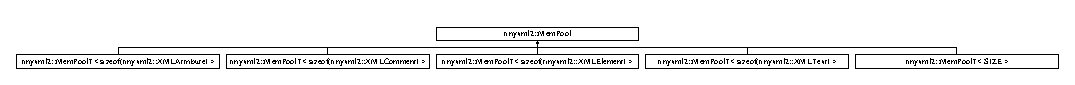
\includegraphics[height=0.691358cm]{classtinyxml2_1_1_mem_pool}
\end{center}
\end{figure}
\subsection*{Public Member Functions}
\begin{DoxyCompactItemize}
\item 
\hyperlink{classtinyxml2_1_1_mem_pool_a9101a0083d7370c85bd5aaaba7157f84}{Mem\-Pool} ()
\item 
virtual \hyperlink{classtinyxml2_1_1_mem_pool_ae55ad9e3faeca702e6ccbb38fdbcad72}{$\sim$\-Mem\-Pool} ()
\item 
virtual int \hyperlink{classtinyxml2_1_1_mem_pool_a0c518d49e3a94bde566f61e13b7240bb}{Item\-Size} () const =0
\item 
virtual void $\ast$ \hyperlink{classtinyxml2_1_1_mem_pool_a4f977b5fed752c0bbfe5295f469d6449}{Alloc} ()=0
\item 
virtual void \hyperlink{classtinyxml2_1_1_mem_pool_a49e3bfac2cba2ebd6776b31e571f64f7}{Free} (void $\ast$)=0
\item 
virtual void \hyperlink{classtinyxml2_1_1_mem_pool_ac5804dd1387b2e4de5eef710076a0db1}{Set\-Tracked} ()=0
\end{DoxyCompactItemize}


\subsection{Constructor \& Destructor Documentation}
\hypertarget{classtinyxml2_1_1_mem_pool_a9101a0083d7370c85bd5aaaba7157f84}{\index{tinyxml2\-::\-Mem\-Pool@{tinyxml2\-::\-Mem\-Pool}!Mem\-Pool@{Mem\-Pool}}
\index{Mem\-Pool@{Mem\-Pool}!tinyxml2::MemPool@{tinyxml2\-::\-Mem\-Pool}}
\subsubsection[{Mem\-Pool}]{\setlength{\rightskip}{0pt plus 5cm}tinyxml2\-::\-Mem\-Pool\-::\-Mem\-Pool (
\begin{DoxyParamCaption}
{}
\end{DoxyParamCaption}
)\hspace{0.3cm}{\ttfamily [inline]}}}\label{classtinyxml2_1_1_mem_pool_a9101a0083d7370c85bd5aaaba7157f84}
\hypertarget{classtinyxml2_1_1_mem_pool_ae55ad9e3faeca702e6ccbb38fdbcad72}{\index{tinyxml2\-::\-Mem\-Pool@{tinyxml2\-::\-Mem\-Pool}!$\sim$\-Mem\-Pool@{$\sim$\-Mem\-Pool}}
\index{$\sim$\-Mem\-Pool@{$\sim$\-Mem\-Pool}!tinyxml2::MemPool@{tinyxml2\-::\-Mem\-Pool}}
\subsubsection[{$\sim$\-Mem\-Pool}]{\setlength{\rightskip}{0pt plus 5cm}virtual tinyxml2\-::\-Mem\-Pool\-::$\sim$\-Mem\-Pool (
\begin{DoxyParamCaption}
{}
\end{DoxyParamCaption}
)\hspace{0.3cm}{\ttfamily [inline]}, {\ttfamily [virtual]}}}\label{classtinyxml2_1_1_mem_pool_ae55ad9e3faeca702e6ccbb38fdbcad72}


\subsection{Member Function Documentation}
\hypertarget{classtinyxml2_1_1_mem_pool_a4f977b5fed752c0bbfe5295f469d6449}{\index{tinyxml2\-::\-Mem\-Pool@{tinyxml2\-::\-Mem\-Pool}!Alloc@{Alloc}}
\index{Alloc@{Alloc}!tinyxml2::MemPool@{tinyxml2\-::\-Mem\-Pool}}
\subsubsection[{Alloc}]{\setlength{\rightskip}{0pt plus 5cm}virtual void$\ast$ tinyxml2\-::\-Mem\-Pool\-::\-Alloc (
\begin{DoxyParamCaption}
{}
\end{DoxyParamCaption}
)\hspace{0.3cm}{\ttfamily [pure virtual]}}}\label{classtinyxml2_1_1_mem_pool_a4f977b5fed752c0bbfe5295f469d6449}


Implemented in \hyperlink{classtinyxml2_1_1_mem_pool_t_aa9d785a48ffe6ea1be679bab13464486}{tinyxml2\-::\-Mem\-Pool\-T$<$ S\-I\-Z\-E $>$}, \hyperlink{classtinyxml2_1_1_mem_pool_t_aa9d785a48ffe6ea1be679bab13464486}{tinyxml2\-::\-Mem\-Pool\-T$<$ sizeof(tinyxml2\-::\-X\-M\-L\-Comment) $>$}, \hyperlink{classtinyxml2_1_1_mem_pool_t_aa9d785a48ffe6ea1be679bab13464486}{tinyxml2\-::\-Mem\-Pool\-T$<$ sizeof(tinyxml2\-::\-X\-M\-L\-Text) $>$}, \hyperlink{classtinyxml2_1_1_mem_pool_t_aa9d785a48ffe6ea1be679bab13464486}{tinyxml2\-::\-Mem\-Pool\-T$<$ sizeof(tinyxml2\-::\-X\-M\-L\-Attribute) $>$}, and \hyperlink{classtinyxml2_1_1_mem_pool_t_aa9d785a48ffe6ea1be679bab13464486}{tinyxml2\-::\-Mem\-Pool\-T$<$ sizeof(tinyxml2\-::\-X\-M\-L\-Element) $>$}.

\hypertarget{classtinyxml2_1_1_mem_pool_a49e3bfac2cba2ebd6776b31e571f64f7}{\index{tinyxml2\-::\-Mem\-Pool@{tinyxml2\-::\-Mem\-Pool}!Free@{Free}}
\index{Free@{Free}!tinyxml2::MemPool@{tinyxml2\-::\-Mem\-Pool}}
\subsubsection[{Free}]{\setlength{\rightskip}{0pt plus 5cm}virtual void tinyxml2\-::\-Mem\-Pool\-::\-Free (
\begin{DoxyParamCaption}
\item[{void $\ast$}]{}
\end{DoxyParamCaption}
)\hspace{0.3cm}{\ttfamily [pure virtual]}}}\label{classtinyxml2_1_1_mem_pool_a49e3bfac2cba2ebd6776b31e571f64f7}


Implemented in \hyperlink{classtinyxml2_1_1_mem_pool_t_a4f1a0c434e9e3d7391e5c16ed4ee8c70}{tinyxml2\-::\-Mem\-Pool\-T$<$ S\-I\-Z\-E $>$}, \hyperlink{classtinyxml2_1_1_mem_pool_t_a4f1a0c434e9e3d7391e5c16ed4ee8c70}{tinyxml2\-::\-Mem\-Pool\-T$<$ sizeof(tinyxml2\-::\-X\-M\-L\-Comment) $>$}, \hyperlink{classtinyxml2_1_1_mem_pool_t_a4f1a0c434e9e3d7391e5c16ed4ee8c70}{tinyxml2\-::\-Mem\-Pool\-T$<$ sizeof(tinyxml2\-::\-X\-M\-L\-Text) $>$}, \hyperlink{classtinyxml2_1_1_mem_pool_t_a4f1a0c434e9e3d7391e5c16ed4ee8c70}{tinyxml2\-::\-Mem\-Pool\-T$<$ sizeof(tinyxml2\-::\-X\-M\-L\-Attribute) $>$}, and \hyperlink{classtinyxml2_1_1_mem_pool_t_a4f1a0c434e9e3d7391e5c16ed4ee8c70}{tinyxml2\-::\-Mem\-Pool\-T$<$ sizeof(tinyxml2\-::\-X\-M\-L\-Element) $>$}.

\hypertarget{classtinyxml2_1_1_mem_pool_a0c518d49e3a94bde566f61e13b7240bb}{\index{tinyxml2\-::\-Mem\-Pool@{tinyxml2\-::\-Mem\-Pool}!Item\-Size@{Item\-Size}}
\index{Item\-Size@{Item\-Size}!tinyxml2::MemPool@{tinyxml2\-::\-Mem\-Pool}}
\subsubsection[{Item\-Size}]{\setlength{\rightskip}{0pt plus 5cm}virtual int tinyxml2\-::\-Mem\-Pool\-::\-Item\-Size (
\begin{DoxyParamCaption}
{}
\end{DoxyParamCaption}
) const\hspace{0.3cm}{\ttfamily [pure virtual]}}}\label{classtinyxml2_1_1_mem_pool_a0c518d49e3a94bde566f61e13b7240bb}


Implemented in \hyperlink{classtinyxml2_1_1_mem_pool_t_a7ec8778fe99f6e332615a703be0b48bc}{tinyxml2\-::\-Mem\-Pool\-T$<$ S\-I\-Z\-E $>$}, \hyperlink{classtinyxml2_1_1_mem_pool_t_a7ec8778fe99f6e332615a703be0b48bc}{tinyxml2\-::\-Mem\-Pool\-T$<$ sizeof(tinyxml2\-::\-X\-M\-L\-Comment) $>$}, \hyperlink{classtinyxml2_1_1_mem_pool_t_a7ec8778fe99f6e332615a703be0b48bc}{tinyxml2\-::\-Mem\-Pool\-T$<$ sizeof(tinyxml2\-::\-X\-M\-L\-Text) $>$}, \hyperlink{classtinyxml2_1_1_mem_pool_t_a7ec8778fe99f6e332615a703be0b48bc}{tinyxml2\-::\-Mem\-Pool\-T$<$ sizeof(tinyxml2\-::\-X\-M\-L\-Attribute) $>$}, and \hyperlink{classtinyxml2_1_1_mem_pool_t_a7ec8778fe99f6e332615a703be0b48bc}{tinyxml2\-::\-Mem\-Pool\-T$<$ sizeof(tinyxml2\-::\-X\-M\-L\-Element) $>$}.

\hypertarget{classtinyxml2_1_1_mem_pool_ac5804dd1387b2e4de5eef710076a0db1}{\index{tinyxml2\-::\-Mem\-Pool@{tinyxml2\-::\-Mem\-Pool}!Set\-Tracked@{Set\-Tracked}}
\index{Set\-Tracked@{Set\-Tracked}!tinyxml2::MemPool@{tinyxml2\-::\-Mem\-Pool}}
\subsubsection[{Set\-Tracked}]{\setlength{\rightskip}{0pt plus 5cm}virtual void tinyxml2\-::\-Mem\-Pool\-::\-Set\-Tracked (
\begin{DoxyParamCaption}
{}
\end{DoxyParamCaption}
)\hspace{0.3cm}{\ttfamily [pure virtual]}}}\label{classtinyxml2_1_1_mem_pool_ac5804dd1387b2e4de5eef710076a0db1}


Implemented in \hyperlink{classtinyxml2_1_1_mem_pool_t_a7798932414916199a1bc0f9c3f368521}{tinyxml2\-::\-Mem\-Pool\-T$<$ S\-I\-Z\-E $>$}, \hyperlink{classtinyxml2_1_1_mem_pool_t_a7798932414916199a1bc0f9c3f368521}{tinyxml2\-::\-Mem\-Pool\-T$<$ sizeof(tinyxml2\-::\-X\-M\-L\-Comment) $>$}, \hyperlink{classtinyxml2_1_1_mem_pool_t_a7798932414916199a1bc0f9c3f368521}{tinyxml2\-::\-Mem\-Pool\-T$<$ sizeof(tinyxml2\-::\-X\-M\-L\-Text) $>$}, \hyperlink{classtinyxml2_1_1_mem_pool_t_a7798932414916199a1bc0f9c3f368521}{tinyxml2\-::\-Mem\-Pool\-T$<$ sizeof(tinyxml2\-::\-X\-M\-L\-Attribute) $>$}, and \hyperlink{classtinyxml2_1_1_mem_pool_t_a7798932414916199a1bc0f9c3f368521}{tinyxml2\-::\-Mem\-Pool\-T$<$ sizeof(tinyxml2\-::\-X\-M\-L\-Element) $>$}.



The documentation for this class was generated from the following file\-:\begin{DoxyCompactItemize}
\item 
Joes\-\_\-\-S\-D\-L\-\_\-\-Framework/\hyperlink{tinyxml2_8h}{tinyxml2.\-h}\end{DoxyCompactItemize}

\hypertarget{classtinyxml2_1_1_mem_pool_t}{\section{tinyxml2\-:\-:Mem\-Pool\-T$<$ S\-I\-Z\-E $>$ Class Template Reference}
\label{classtinyxml2_1_1_mem_pool_t}\index{tinyxml2\-::\-Mem\-Pool\-T$<$ S\-I\-Z\-E $>$@{tinyxml2\-::\-Mem\-Pool\-T$<$ S\-I\-Z\-E $>$}}
}
Inheritance diagram for tinyxml2\-:\-:Mem\-Pool\-T$<$ S\-I\-Z\-E $>$\-:\begin{figure}[H]
\begin{center}
\leavevmode
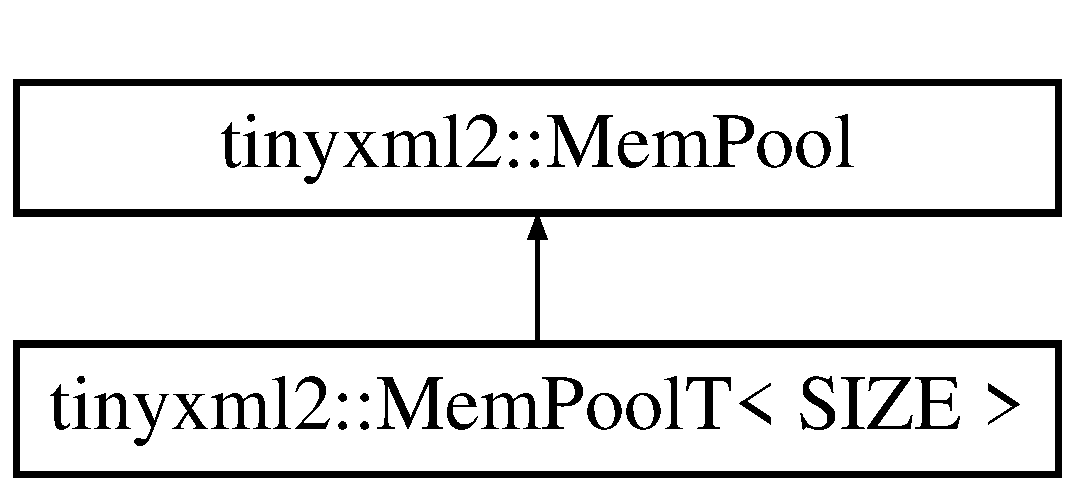
\includegraphics[height=2.000000cm]{classtinyxml2_1_1_mem_pool_t}
\end{center}
\end{figure}
\subsection*{Public Types}
\begin{DoxyCompactItemize}
\item 
enum \{ {\bfseries C\-O\-U\-N\-T} = (4$\ast$1024)/\-S\-I\-Z\-E
 \}
\end{DoxyCompactItemize}
\subsection*{Public Member Functions}
\begin{DoxyCompactItemize}
\item 
\hypertarget{classtinyxml2_1_1_mem_pool_t_a7ec8778fe99f6e332615a703be0b48bc}{virtual int {\bfseries Item\-Size} () const }\label{classtinyxml2_1_1_mem_pool_t_a7ec8778fe99f6e332615a703be0b48bc}

\item 
\hypertarget{classtinyxml2_1_1_mem_pool_t_a56be11b7db6a7ef00db17088a7769aab}{int {\bfseries Current\-Allocs} () const }\label{classtinyxml2_1_1_mem_pool_t_a56be11b7db6a7ef00db17088a7769aab}

\item 
\hypertarget{classtinyxml2_1_1_mem_pool_t_aa9d785a48ffe6ea1be679bab13464486}{virtual void $\ast$ {\bfseries Alloc} ()}\label{classtinyxml2_1_1_mem_pool_t_aa9d785a48ffe6ea1be679bab13464486}

\item 
\hypertarget{classtinyxml2_1_1_mem_pool_t_a4f1a0c434e9e3d7391e5c16ed4ee8c70}{virtual void {\bfseries Free} (void $\ast$mem)}\label{classtinyxml2_1_1_mem_pool_t_a4f1a0c434e9e3d7391e5c16ed4ee8c70}

\item 
\hypertarget{classtinyxml2_1_1_mem_pool_t_a0bc596f271e0f139822c534238b3f244}{void {\bfseries Trace} (const char $\ast$name)}\label{classtinyxml2_1_1_mem_pool_t_a0bc596f271e0f139822c534238b3f244}

\item 
\hypertarget{classtinyxml2_1_1_mem_pool_t_a7798932414916199a1bc0f9c3f368521}{void {\bfseries Set\-Tracked} ()}\label{classtinyxml2_1_1_mem_pool_t_a7798932414916199a1bc0f9c3f368521}

\item 
\hypertarget{classtinyxml2_1_1_mem_pool_t_a524b90d0edeac41964c06510757dce0f}{int {\bfseries Untracked} () const }\label{classtinyxml2_1_1_mem_pool_t_a524b90d0edeac41964c06510757dce0f}

\end{DoxyCompactItemize}


The documentation for this class was generated from the following file\-:\begin{DoxyCompactItemize}
\item 
Joes\-\_\-\-S\-D\-L\-\_\-\-Framework/tinyxml2.\-h\end{DoxyCompactItemize}

\hypertarget{class_player}{\section{Player Class Reference}
\label{class_player}\index{Player@{Player}}
}


{\ttfamily \#include $<$Player.\-h$>$}

Inheritance diagram for Player\-:\begin{figure}[H]
\begin{center}
\leavevmode
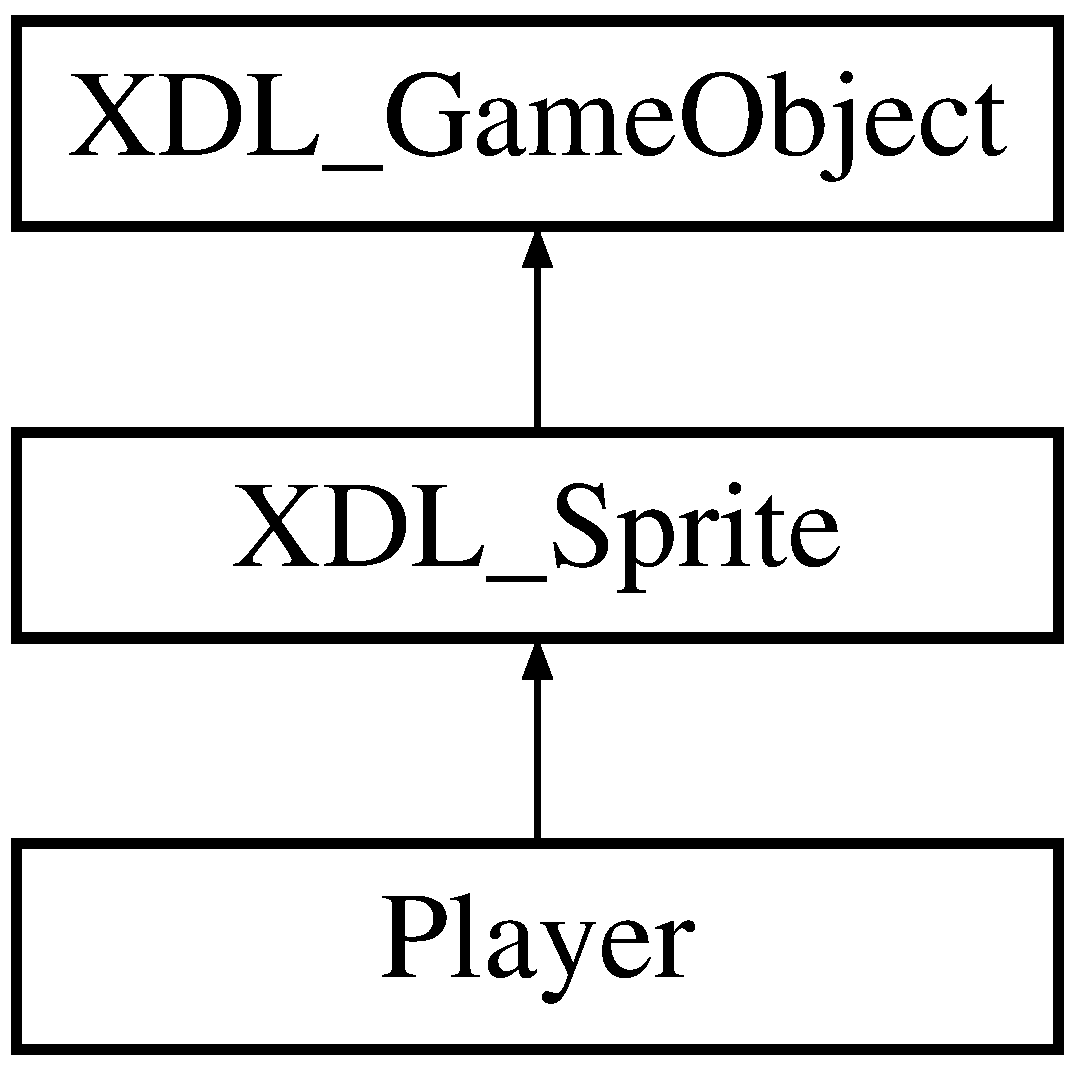
\includegraphics[height=3.000000cm]{class_player}
\end{center}
\end{figure}
\subsection*{Public Member Functions}
\begin{DoxyCompactItemize}
\item 
\hyperlink{class_player_a6441995ccc3600a6d8351abbbb5968e2}{Player} (S\-D\-L\-\_\-\-Renderer $\ast$\hyperlink{class_x_d_l___sprite_aedcf07ef73df095eb6cd9843870cd002}{\-\_\-renderer}, char $\ast$\-\_\-asset, S\-D\-L\-\_\-\-Rect \-\_\-rect, int \hyperlink{class_x_d_l___sprite_ac7671bf39741642f55368690a562fff8}{\-\_\-pos\-X}, int \hyperlink{class_x_d_l___sprite_a2e69aab364da9c9e16ae398838679065}{\-\_\-pos\-Y}, \hyperlink{class_x_d_l___path_finder}{X\-D\-L\-\_\-\-Path\-Finder} $\ast$\-\_\-path\-Finder, \hyperlink{class_x_d_l___sprite}{X\-D\-L\-\_\-\-Sprite} $\ast$\-\_\-target, int \-\_\-r, int \-\_\-g, int \-\_\-b, int \-\_\-a)
\item 
virtual \hyperlink{class_player_a949762ad57300f070d83ec877ec6e907}{$\sim$\-Player} (void)
\item 
void \hyperlink{class_player_a456327628e5ee73666add176752b36fe}{Stop\-Following\-Path} ()
\item 
void \hyperlink{class_player_a7a8ac5183d635f6f49cc1bdf285953c2}{Follow\-Path} (vector$<$ S\-D\-L\-\_\-\-Point $\ast$ $>$ $\ast$\-\_\-path)
\item 
int \hyperlink{class_player_ac7e6dc6806a9f5ddae4f5a015f8cac27}{Distance\-From} (int \-\_\-start\-X, int \-\_\-start\-Y, int \-\_\-end\-X, int \-\_\-end\-Y)
\item 
void \hyperlink{class_player_a05b60cac1922c5be5c1be16baffa4497}{Update} ()
\item 
void \hyperlink{class_player_a00ae3ebe88af8f9cfabd819176516a73}{Draw} ()
\end{DoxyCompactItemize}
\subsection*{Public Attributes}
\begin{DoxyCompactItemize}
\item 
bool \hyperlink{class_player_a8e8d189f49c664445fba0976115bb030}{\-\_\-follow\-Path}
\end{DoxyCompactItemize}
\subsection*{Static Public Attributes}
\begin{DoxyCompactItemize}
\item 
static bool \hyperlink{class_player_a39c12b1c083f02ba270fd7c2c4d48e42}{\-\_\-locked}
\end{DoxyCompactItemize}
\subsection*{Additional Inherited Members}


\subsection{Constructor \& Destructor Documentation}
\hypertarget{class_player_a6441995ccc3600a6d8351abbbb5968e2}{\index{Player@{Player}!Player@{Player}}
\index{Player@{Player}!Player@{Player}}
\subsubsection[{Player}]{\setlength{\rightskip}{0pt plus 5cm}Player\-::\-Player (
\begin{DoxyParamCaption}
\item[{S\-D\-L\-\_\-\-Renderer $\ast$}]{\-\_\-renderer, }
\item[{char $\ast$}]{\-\_\-asset, }
\item[{S\-D\-L\-\_\-\-Rect}]{\-\_\-rect, }
\item[{int}]{\-\_\-pos\-X, }
\item[{int}]{\-\_\-pos\-Y, }
\item[{{\bf X\-D\-L\-\_\-\-Path\-Finder} $\ast$}]{\-\_\-path\-Finder, }
\item[{{\bf X\-D\-L\-\_\-\-Sprite} $\ast$}]{\-\_\-target, }
\item[{int}]{\-\_\-r, }
\item[{int}]{\-\_\-g, }
\item[{int}]{\-\_\-b, }
\item[{int}]{\-\_\-a}
\end{DoxyParamCaption}
)}}\label{class_player_a6441995ccc3600a6d8351abbbb5968e2}
\hypertarget{class_player_a949762ad57300f070d83ec877ec6e907}{\index{Player@{Player}!$\sim$\-Player@{$\sim$\-Player}}
\index{$\sim$\-Player@{$\sim$\-Player}!Player@{Player}}
\subsubsection[{$\sim$\-Player}]{\setlength{\rightskip}{0pt plus 5cm}Player\-::$\sim$\-Player (
\begin{DoxyParamCaption}
\item[{void}]{}
\end{DoxyParamCaption}
)\hspace{0.3cm}{\ttfamily [virtual]}}}\label{class_player_a949762ad57300f070d83ec877ec6e907}


\subsection{Member Function Documentation}
\hypertarget{class_player_ac7e6dc6806a9f5ddae4f5a015f8cac27}{\index{Player@{Player}!Distance\-From@{Distance\-From}}
\index{Distance\-From@{Distance\-From}!Player@{Player}}
\subsubsection[{Distance\-From}]{\setlength{\rightskip}{0pt plus 5cm}int Player\-::\-Distance\-From (
\begin{DoxyParamCaption}
\item[{int}]{\-\_\-start\-X, }
\item[{int}]{\-\_\-start\-Y, }
\item[{int}]{\-\_\-end\-X, }
\item[{int}]{\-\_\-end\-Y}
\end{DoxyParamCaption}
)}}\label{class_player_ac7e6dc6806a9f5ddae4f5a015f8cac27}
\hypertarget{class_player_a00ae3ebe88af8f9cfabd819176516a73}{\index{Player@{Player}!Draw@{Draw}}
\index{Draw@{Draw}!Player@{Player}}
\subsubsection[{Draw}]{\setlength{\rightskip}{0pt plus 5cm}void Player\-::\-Draw (
\begin{DoxyParamCaption}
{}
\end{DoxyParamCaption}
)\hspace{0.3cm}{\ttfamily [virtual]}}}\label{class_player_a00ae3ebe88af8f9cfabd819176516a73}
virtual function so every object that is added to the scene will get auto-\/updated 

Reimplemented from \hyperlink{class_x_d_l___sprite_a5b1c9b886c59f06cfbb2c428b3f58e86}{X\-D\-L\-\_\-\-Sprite}.

\hypertarget{class_player_a7a8ac5183d635f6f49cc1bdf285953c2}{\index{Player@{Player}!Follow\-Path@{Follow\-Path}}
\index{Follow\-Path@{Follow\-Path}!Player@{Player}}
\subsubsection[{Follow\-Path}]{\setlength{\rightskip}{0pt plus 5cm}void Player\-::\-Follow\-Path (
\begin{DoxyParamCaption}
\item[{vector$<$ S\-D\-L\-\_\-\-Point $\ast$ $>$ $\ast$}]{\-\_\-path}
\end{DoxyParamCaption}
)}}\label{class_player_a7a8ac5183d635f6f49cc1bdf285953c2}
\hypertarget{class_player_a456327628e5ee73666add176752b36fe}{\index{Player@{Player}!Stop\-Following\-Path@{Stop\-Following\-Path}}
\index{Stop\-Following\-Path@{Stop\-Following\-Path}!Player@{Player}}
\subsubsection[{Stop\-Following\-Path}]{\setlength{\rightskip}{0pt plus 5cm}void Player\-::\-Stop\-Following\-Path (
\begin{DoxyParamCaption}
{}
\end{DoxyParamCaption}
)}}\label{class_player_a456327628e5ee73666add176752b36fe}
\hypertarget{class_player_a05b60cac1922c5be5c1be16baffa4497}{\index{Player@{Player}!Update@{Update}}
\index{Update@{Update}!Player@{Player}}
\subsubsection[{Update}]{\setlength{\rightskip}{0pt plus 5cm}void Player\-::\-Update (
\begin{DoxyParamCaption}
{}
\end{DoxyParamCaption}
)\hspace{0.3cm}{\ttfamily [virtual]}}}\label{class_player_a05b60cac1922c5be5c1be16baffa4497}


Reimplemented from \hyperlink{class_x_d_l___sprite_a1ecd6d713ce320cd1d49dceea854e0d2}{X\-D\-L\-\_\-\-Sprite}.



\subsection{Member Data Documentation}
\hypertarget{class_player_a8e8d189f49c664445fba0976115bb030}{\index{Player@{Player}!\-\_\-follow\-Path@{\-\_\-follow\-Path}}
\index{\-\_\-follow\-Path@{\-\_\-follow\-Path}!Player@{Player}}
\subsubsection[{\-\_\-follow\-Path}]{\setlength{\rightskip}{0pt plus 5cm}bool Player\-::\-\_\-follow\-Path}}\label{class_player_a8e8d189f49c664445fba0976115bb030}
\hypertarget{class_player_a39c12b1c083f02ba270fd7c2c4d48e42}{\index{Player@{Player}!\-\_\-locked@{\-\_\-locked}}
\index{\-\_\-locked@{\-\_\-locked}!Player@{Player}}
\subsubsection[{\-\_\-locked}]{\setlength{\rightskip}{0pt plus 5cm}bool Player\-::\-\_\-locked\hspace{0.3cm}{\ttfamily [static]}}}\label{class_player_a39c12b1c083f02ba270fd7c2c4d48e42}


The documentation for this class was generated from the following files\-:\begin{DoxyCompactItemize}
\item 
Joes\-\_\-\-S\-D\-L\-\_\-\-Framework/\hyperlink{_player_8h}{Player.\-h}\item 
Joes\-\_\-\-S\-D\-L\-\_\-\-Framework/\hyperlink{_player_8cpp}{Player.\-cpp}\end{DoxyCompactItemize}

\hypertarget{class_pokemon_town}{\section{Pokemon\-Town Class Reference}
\label{class_pokemon_town}\index{Pokemon\-Town@{Pokemon\-Town}}
}


{\ttfamily \#include $<$Pokemon\-Town.\-h$>$}

Inheritance diagram for Pokemon\-Town\-:\begin{figure}[H]
\begin{center}
\leavevmode
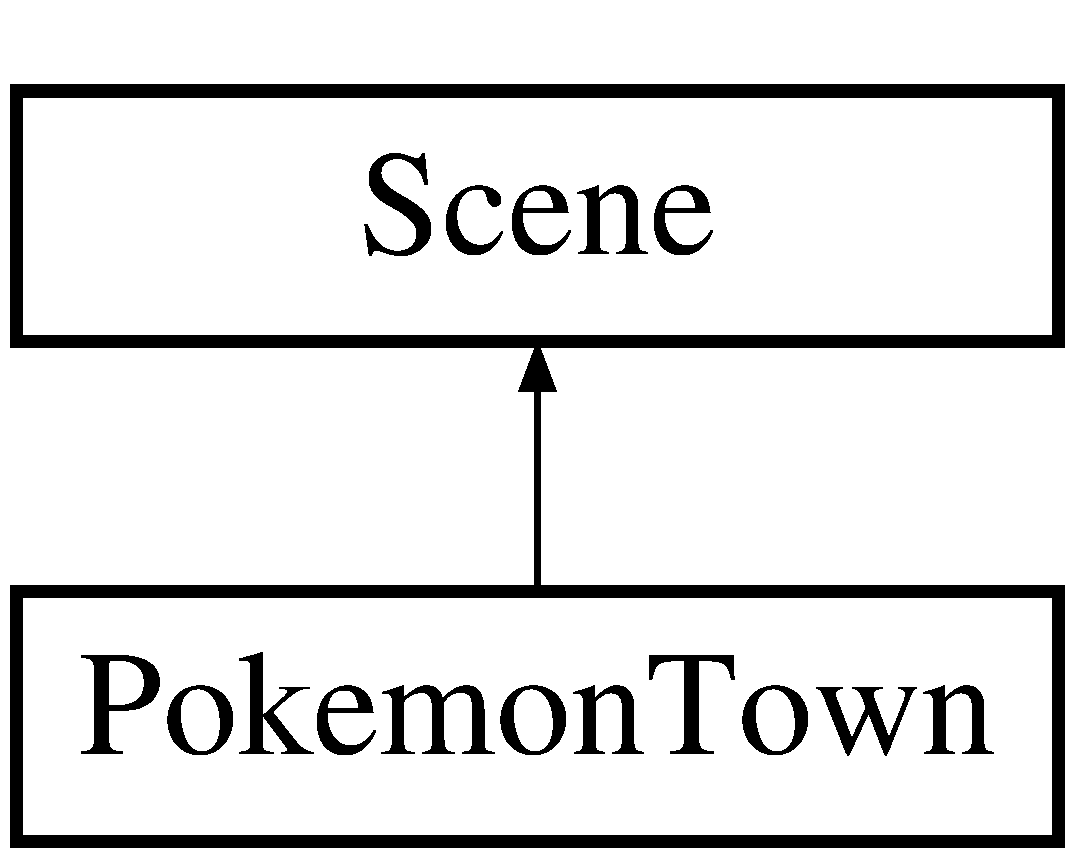
\includegraphics[height=2.000000cm]{class_pokemon_town}
\end{center}
\end{figure}
\subsection*{Public Member Functions}
\begin{DoxyCompactItemize}
\item 
\hyperlink{class_pokemon_town_a999ed4c76a1fa931a6c0acb984d71caf}{Pokemon\-Town} (S\-D\-L\-\_\-\-Renderer $\ast$\-\_\-renderer)
\item 
\hyperlink{class_pokemon_town_af68c21ca9996cd73a35167a290d2ba01}{$\sim$\-Pokemon\-Town} (void)
\item 
void \hyperlink{class_pokemon_town_a72cdaf8645ec395b4ee351dbe3a7c097}{Draw} ()
\item 
void \hyperlink{class_pokemon_town_a61a3f5e9b30126be3fa657d29877d596}{Update} ()
\end{DoxyCompactItemize}


\subsection{Constructor \& Destructor Documentation}
\hypertarget{class_pokemon_town_a999ed4c76a1fa931a6c0acb984d71caf}{\index{Pokemon\-Town@{Pokemon\-Town}!Pokemon\-Town@{Pokemon\-Town}}
\index{Pokemon\-Town@{Pokemon\-Town}!PokemonTown@{Pokemon\-Town}}
\subsubsection[{Pokemon\-Town}]{\setlength{\rightskip}{0pt plus 5cm}Pokemon\-Town\-::\-Pokemon\-Town (
\begin{DoxyParamCaption}
\item[{S\-D\-L\-\_\-\-Renderer $\ast$}]{\-\_\-renderer}
\end{DoxyParamCaption}
)}}\label{class_pokemon_town_a999ed4c76a1fa931a6c0acb984d71caf}
\hypertarget{class_pokemon_town_af68c21ca9996cd73a35167a290d2ba01}{\index{Pokemon\-Town@{Pokemon\-Town}!$\sim$\-Pokemon\-Town@{$\sim$\-Pokemon\-Town}}
\index{$\sim$\-Pokemon\-Town@{$\sim$\-Pokemon\-Town}!PokemonTown@{Pokemon\-Town}}
\subsubsection[{$\sim$\-Pokemon\-Town}]{\setlength{\rightskip}{0pt plus 5cm}Pokemon\-Town\-::$\sim$\-Pokemon\-Town (
\begin{DoxyParamCaption}
\item[{void}]{}
\end{DoxyParamCaption}
)}}\label{class_pokemon_town_af68c21ca9996cd73a35167a290d2ba01}


\subsection{Member Function Documentation}
\hypertarget{class_pokemon_town_a72cdaf8645ec395b4ee351dbe3a7c097}{\index{Pokemon\-Town@{Pokemon\-Town}!Draw@{Draw}}
\index{Draw@{Draw}!PokemonTown@{Pokemon\-Town}}
\subsubsection[{Draw}]{\setlength{\rightskip}{0pt plus 5cm}void Pokemon\-Town\-::\-Draw (
\begin{DoxyParamCaption}
{}
\end{DoxyParamCaption}
)}}\label{class_pokemon_town_a72cdaf8645ec395b4ee351dbe3a7c097}
\hypertarget{class_pokemon_town_a61a3f5e9b30126be3fa657d29877d596}{\index{Pokemon\-Town@{Pokemon\-Town}!Update@{Update}}
\index{Update@{Update}!PokemonTown@{Pokemon\-Town}}
\subsubsection[{Update}]{\setlength{\rightskip}{0pt plus 5cm}void Pokemon\-Town\-::\-Update (
\begin{DoxyParamCaption}
{}
\end{DoxyParamCaption}
)}}\label{class_pokemon_town_a61a3f5e9b30126be3fa657d29877d596}


The documentation for this class was generated from the following file\-:\begin{DoxyCompactItemize}
\item 
Joes\-\_\-\-S\-D\-L\-\_\-\-Framework/\hyperlink{_pokemon_town_8h}{Pokemon\-Town.\-h}\end{DoxyCompactItemize}

\hypertarget{classtinyxml2_1_1_str_pair}{\section{tinyxml2\-:\-:Str\-Pair Class Reference}
\label{classtinyxml2_1_1_str_pair}\index{tinyxml2\-::\-Str\-Pair@{tinyxml2\-::\-Str\-Pair}}
}


{\ttfamily \#include $<$tinyxml2.\-h$>$}

\subsection*{Public Types}
\begin{DoxyCompactItemize}
\item 
enum \{ \\*
\hyperlink{classtinyxml2_1_1_str_pair_a0301ef962e15dd94574431f1c61266c5a4f1e01a55f8efe4ca72c32d454060237}{N\-E\-E\-D\-S\-\_\-\-E\-N\-T\-I\-T\-Y\-\_\-\-P\-R\-O\-C\-E\-S\-S\-I\-N\-G} = 0x01, 
\hyperlink{classtinyxml2_1_1_str_pair_a0301ef962e15dd94574431f1c61266c5a8f2045d56e70745d718672c0da91d0e0}{N\-E\-E\-D\-S\-\_\-\-N\-E\-W\-L\-I\-N\-E\-\_\-\-N\-O\-R\-M\-A\-L\-I\-Z\-A\-T\-I\-O\-N} = 0x02, 
\hyperlink{classtinyxml2_1_1_str_pair_a0301ef962e15dd94574431f1c61266c5ab17a85f396c221811fe49263bf6f843f}{C\-O\-L\-L\-A\-P\-S\-E\-\_\-\-W\-H\-I\-T\-E\-S\-P\-A\-C\-E} = 0x04, 
\hyperlink{classtinyxml2_1_1_str_pair_a0301ef962e15dd94574431f1c61266c5aae519eb5a639858591763aa5fc6cc953}{T\-E\-X\-T\-\_\-\-E\-L\-E\-M\-E\-N\-T} = N\-E\-E\-D\-S\-\_\-\-E\-N\-T\-I\-T\-Y\-\_\-\-P\-R\-O\-C\-E\-S\-S\-I\-N\-G $\vert$ N\-E\-E\-D\-S\-\_\-\-N\-E\-W\-L\-I\-N\-E\-\_\-\-N\-O\-R\-M\-A\-L\-I\-Z\-A\-T\-I\-O\-N, 
\\*
\hyperlink{classtinyxml2_1_1_str_pair_a0301ef962e15dd94574431f1c61266c5a96be48cf899bfeea0aa227f984f1fa63}{T\-E\-X\-T\-\_\-\-E\-L\-E\-M\-E\-N\-T\-\_\-\-L\-E\-A\-V\-E\-\_\-\-E\-N\-T\-I\-T\-I\-E\-S} = N\-E\-E\-D\-S\-\_\-\-N\-E\-W\-L\-I\-N\-E\-\_\-\-N\-O\-R\-M\-A\-L\-I\-Z\-A\-T\-I\-O\-N, 
\hyperlink{classtinyxml2_1_1_str_pair_a0301ef962e15dd94574431f1c61266c5aaab1cbefaa977e6f772b4e2575417aeb}{A\-T\-T\-R\-I\-B\-U\-T\-E\-\_\-\-N\-A\-M\-E} = 0, 
\hyperlink{classtinyxml2_1_1_str_pair_a0301ef962e15dd94574431f1c61266c5a6d72f9ce15f50e8bcd680edf66235dfd}{A\-T\-T\-R\-I\-B\-U\-T\-E\-\_\-\-V\-A\-L\-U\-E} = N\-E\-E\-D\-S\-\_\-\-E\-N\-T\-I\-T\-Y\-\_\-\-P\-R\-O\-C\-E\-S\-S\-I\-N\-G $\vert$ N\-E\-E\-D\-S\-\_\-\-N\-E\-W\-L\-I\-N\-E\-\_\-\-N\-O\-R\-M\-A\-L\-I\-Z\-A\-T\-I\-O\-N, 
\hyperlink{classtinyxml2_1_1_str_pair_a0301ef962e15dd94574431f1c61266c5a2decbd2513ac14f8befa987938326399}{A\-T\-T\-R\-I\-B\-U\-T\-E\-\_\-\-V\-A\-L\-U\-E\-\_\-\-L\-E\-A\-V\-E\-\_\-\-E\-N\-T\-I\-T\-I\-E\-S} = N\-E\-E\-D\-S\-\_\-\-N\-E\-W\-L\-I\-N\-E\-\_\-\-N\-O\-R\-M\-A\-L\-I\-Z\-A\-T\-I\-O\-N, 
\\*
\hyperlink{classtinyxml2_1_1_str_pair_a0301ef962e15dd94574431f1c61266c5a067a6ec90c8beea1cf5992930d93bffa}{C\-O\-M\-M\-E\-N\-T} = N\-E\-E\-D\-S\-\_\-\-N\-E\-W\-L\-I\-N\-E\-\_\-\-N\-O\-R\-M\-A\-L\-I\-Z\-A\-T\-I\-O\-N
 \}
\end{DoxyCompactItemize}
\subsection*{Public Member Functions}
\begin{DoxyCompactItemize}
\item 
\hyperlink{classtinyxml2_1_1_str_pair_a69153963f7052de9f767d3d8c1623a70}{Str\-Pair} ()
\item 
\hyperlink{classtinyxml2_1_1_str_pair_a60bed84d2503296e1c2a73fcef1431f9}{$\sim$\-Str\-Pair} ()
\item 
void \hyperlink{classtinyxml2_1_1_str_pair_a4f05549373394266a1eecba26813c166}{Set} (char $\ast$\hyperlink{_x_d_l___main_8cpp_a2182b4f4175ea78bf91a9b7a78fa1c0a}{start}, char $\ast$end, int flags)
\item 
const char $\ast$ \hyperlink{classtinyxml2_1_1_str_pair_ad87e3d11330f5e689ba1e7e54c023b57}{Get\-Str} ()
\item 
bool \hyperlink{classtinyxml2_1_1_str_pair_affa1043e73a18f05d5d2faec055725a7}{Empty} () const 
\item 
void \hyperlink{classtinyxml2_1_1_str_pair_a2baf6230e18333e02ab65d0897ee3941}{Set\-Interned\-Str} (const char $\ast$str)
\item 
void \hyperlink{classtinyxml2_1_1_str_pair_a1f82ec6b5bee35ee7466d8565e43b1de}{Set\-Str} (const char $\ast$str, int flags=0)
\item 
char $\ast$ \hyperlink{classtinyxml2_1_1_str_pair_ad90521f188e9606a8fbafe5d86fb2246}{Parse\-Text} (char $\ast$in, const char $\ast$end\-Tag, int str\-Flags)
\item 
char $\ast$ \hyperlink{classtinyxml2_1_1_str_pair_aa6d8998efceba41d87ec2300c70a6085}{Parse\-Name} (char $\ast$in)
\end{DoxyCompactItemize}


\subsection{Member Enumeration Documentation}
\hypertarget{classtinyxml2_1_1_str_pair_a0301ef962e15dd94574431f1c61266c5}{\subsubsection[{anonymous enum}]{\setlength{\rightskip}{0pt plus 5cm}anonymous enum}}\label{classtinyxml2_1_1_str_pair_a0301ef962e15dd94574431f1c61266c5}
\begin{Desc}
\item[Enumerator]\par
\begin{description}
\index{N\-E\-E\-D\-S\-\_\-\-E\-N\-T\-I\-T\-Y\-\_\-\-P\-R\-O\-C\-E\-S\-S\-I\-N\-G@{N\-E\-E\-D\-S\-\_\-\-E\-N\-T\-I\-T\-Y\-\_\-\-P\-R\-O\-C\-E\-S\-S\-I\-N\-G}!tinyxml2\-::\-Str\-Pair@{tinyxml2\-::\-Str\-Pair}}\index{tinyxml2\-::\-Str\-Pair@{tinyxml2\-::\-Str\-Pair}!N\-E\-E\-D\-S\-\_\-\-E\-N\-T\-I\-T\-Y\-\_\-\-P\-R\-O\-C\-E\-S\-S\-I\-N\-G@{N\-E\-E\-D\-S\-\_\-\-E\-N\-T\-I\-T\-Y\-\_\-\-P\-R\-O\-C\-E\-S\-S\-I\-N\-G}}\item[{\em 
\hypertarget{classtinyxml2_1_1_str_pair_a0301ef962e15dd94574431f1c61266c5a4f1e01a55f8efe4ca72c32d454060237}{N\-E\-E\-D\-S\-\_\-\-E\-N\-T\-I\-T\-Y\-\_\-\-P\-R\-O\-C\-E\-S\-S\-I\-N\-G}\label{classtinyxml2_1_1_str_pair_a0301ef962e15dd94574431f1c61266c5a4f1e01a55f8efe4ca72c32d454060237}
}]\index{N\-E\-E\-D\-S\-\_\-\-N\-E\-W\-L\-I\-N\-E\-\_\-\-N\-O\-R\-M\-A\-L\-I\-Z\-A\-T\-I\-O\-N@{N\-E\-E\-D\-S\-\_\-\-N\-E\-W\-L\-I\-N\-E\-\_\-\-N\-O\-R\-M\-A\-L\-I\-Z\-A\-T\-I\-O\-N}!tinyxml2\-::\-Str\-Pair@{tinyxml2\-::\-Str\-Pair}}\index{tinyxml2\-::\-Str\-Pair@{tinyxml2\-::\-Str\-Pair}!N\-E\-E\-D\-S\-\_\-\-N\-E\-W\-L\-I\-N\-E\-\_\-\-N\-O\-R\-M\-A\-L\-I\-Z\-A\-T\-I\-O\-N@{N\-E\-E\-D\-S\-\_\-\-N\-E\-W\-L\-I\-N\-E\-\_\-\-N\-O\-R\-M\-A\-L\-I\-Z\-A\-T\-I\-O\-N}}\item[{\em 
\hypertarget{classtinyxml2_1_1_str_pair_a0301ef962e15dd94574431f1c61266c5a8f2045d56e70745d718672c0da91d0e0}{N\-E\-E\-D\-S\-\_\-\-N\-E\-W\-L\-I\-N\-E\-\_\-\-N\-O\-R\-M\-A\-L\-I\-Z\-A\-T\-I\-O\-N}\label{classtinyxml2_1_1_str_pair_a0301ef962e15dd94574431f1c61266c5a8f2045d56e70745d718672c0da91d0e0}
}]\index{C\-O\-L\-L\-A\-P\-S\-E\-\_\-\-W\-H\-I\-T\-E\-S\-P\-A\-C\-E@{C\-O\-L\-L\-A\-P\-S\-E\-\_\-\-W\-H\-I\-T\-E\-S\-P\-A\-C\-E}!tinyxml2\-::\-Str\-Pair@{tinyxml2\-::\-Str\-Pair}}\index{tinyxml2\-::\-Str\-Pair@{tinyxml2\-::\-Str\-Pair}!C\-O\-L\-L\-A\-P\-S\-E\-\_\-\-W\-H\-I\-T\-E\-S\-P\-A\-C\-E@{C\-O\-L\-L\-A\-P\-S\-E\-\_\-\-W\-H\-I\-T\-E\-S\-P\-A\-C\-E}}\item[{\em 
\hypertarget{classtinyxml2_1_1_str_pair_a0301ef962e15dd94574431f1c61266c5ab17a85f396c221811fe49263bf6f843f}{C\-O\-L\-L\-A\-P\-S\-E\-\_\-\-W\-H\-I\-T\-E\-S\-P\-A\-C\-E}\label{classtinyxml2_1_1_str_pair_a0301ef962e15dd94574431f1c61266c5ab17a85f396c221811fe49263bf6f843f}
}]\index{T\-E\-X\-T\-\_\-\-E\-L\-E\-M\-E\-N\-T@{T\-E\-X\-T\-\_\-\-E\-L\-E\-M\-E\-N\-T}!tinyxml2\-::\-Str\-Pair@{tinyxml2\-::\-Str\-Pair}}\index{tinyxml2\-::\-Str\-Pair@{tinyxml2\-::\-Str\-Pair}!T\-E\-X\-T\-\_\-\-E\-L\-E\-M\-E\-N\-T@{T\-E\-X\-T\-\_\-\-E\-L\-E\-M\-E\-N\-T}}\item[{\em 
\hypertarget{classtinyxml2_1_1_str_pair_a0301ef962e15dd94574431f1c61266c5aae519eb5a639858591763aa5fc6cc953}{T\-E\-X\-T\-\_\-\-E\-L\-E\-M\-E\-N\-T}\label{classtinyxml2_1_1_str_pair_a0301ef962e15dd94574431f1c61266c5aae519eb5a639858591763aa5fc6cc953}
}]\index{T\-E\-X\-T\-\_\-\-E\-L\-E\-M\-E\-N\-T\-\_\-\-L\-E\-A\-V\-E\-\_\-\-E\-N\-T\-I\-T\-I\-E\-S@{T\-E\-X\-T\-\_\-\-E\-L\-E\-M\-E\-N\-T\-\_\-\-L\-E\-A\-V\-E\-\_\-\-E\-N\-T\-I\-T\-I\-E\-S}!tinyxml2\-::\-Str\-Pair@{tinyxml2\-::\-Str\-Pair}}\index{tinyxml2\-::\-Str\-Pair@{tinyxml2\-::\-Str\-Pair}!T\-E\-X\-T\-\_\-\-E\-L\-E\-M\-E\-N\-T\-\_\-\-L\-E\-A\-V\-E\-\_\-\-E\-N\-T\-I\-T\-I\-E\-S@{T\-E\-X\-T\-\_\-\-E\-L\-E\-M\-E\-N\-T\-\_\-\-L\-E\-A\-V\-E\-\_\-\-E\-N\-T\-I\-T\-I\-E\-S}}\item[{\em 
\hypertarget{classtinyxml2_1_1_str_pair_a0301ef962e15dd94574431f1c61266c5a96be48cf899bfeea0aa227f984f1fa63}{T\-E\-X\-T\-\_\-\-E\-L\-E\-M\-E\-N\-T\-\_\-\-L\-E\-A\-V\-E\-\_\-\-E\-N\-T\-I\-T\-I\-E\-S}\label{classtinyxml2_1_1_str_pair_a0301ef962e15dd94574431f1c61266c5a96be48cf899bfeea0aa227f984f1fa63}
}]\index{A\-T\-T\-R\-I\-B\-U\-T\-E\-\_\-\-N\-A\-M\-E@{A\-T\-T\-R\-I\-B\-U\-T\-E\-\_\-\-N\-A\-M\-E}!tinyxml2\-::\-Str\-Pair@{tinyxml2\-::\-Str\-Pair}}\index{tinyxml2\-::\-Str\-Pair@{tinyxml2\-::\-Str\-Pair}!A\-T\-T\-R\-I\-B\-U\-T\-E\-\_\-\-N\-A\-M\-E@{A\-T\-T\-R\-I\-B\-U\-T\-E\-\_\-\-N\-A\-M\-E}}\item[{\em 
\hypertarget{classtinyxml2_1_1_str_pair_a0301ef962e15dd94574431f1c61266c5aaab1cbefaa977e6f772b4e2575417aeb}{A\-T\-T\-R\-I\-B\-U\-T\-E\-\_\-\-N\-A\-M\-E}\label{classtinyxml2_1_1_str_pair_a0301ef962e15dd94574431f1c61266c5aaab1cbefaa977e6f772b4e2575417aeb}
}]\index{A\-T\-T\-R\-I\-B\-U\-T\-E\-\_\-\-V\-A\-L\-U\-E@{A\-T\-T\-R\-I\-B\-U\-T\-E\-\_\-\-V\-A\-L\-U\-E}!tinyxml2\-::\-Str\-Pair@{tinyxml2\-::\-Str\-Pair}}\index{tinyxml2\-::\-Str\-Pair@{tinyxml2\-::\-Str\-Pair}!A\-T\-T\-R\-I\-B\-U\-T\-E\-\_\-\-V\-A\-L\-U\-E@{A\-T\-T\-R\-I\-B\-U\-T\-E\-\_\-\-V\-A\-L\-U\-E}}\item[{\em 
\hypertarget{classtinyxml2_1_1_str_pair_a0301ef962e15dd94574431f1c61266c5a6d72f9ce15f50e8bcd680edf66235dfd}{A\-T\-T\-R\-I\-B\-U\-T\-E\-\_\-\-V\-A\-L\-U\-E}\label{classtinyxml2_1_1_str_pair_a0301ef962e15dd94574431f1c61266c5a6d72f9ce15f50e8bcd680edf66235dfd}
}]\index{A\-T\-T\-R\-I\-B\-U\-T\-E\-\_\-\-V\-A\-L\-U\-E\-\_\-\-L\-E\-A\-V\-E\-\_\-\-E\-N\-T\-I\-T\-I\-E\-S@{A\-T\-T\-R\-I\-B\-U\-T\-E\-\_\-\-V\-A\-L\-U\-E\-\_\-\-L\-E\-A\-V\-E\-\_\-\-E\-N\-T\-I\-T\-I\-E\-S}!tinyxml2\-::\-Str\-Pair@{tinyxml2\-::\-Str\-Pair}}\index{tinyxml2\-::\-Str\-Pair@{tinyxml2\-::\-Str\-Pair}!A\-T\-T\-R\-I\-B\-U\-T\-E\-\_\-\-V\-A\-L\-U\-E\-\_\-\-L\-E\-A\-V\-E\-\_\-\-E\-N\-T\-I\-T\-I\-E\-S@{A\-T\-T\-R\-I\-B\-U\-T\-E\-\_\-\-V\-A\-L\-U\-E\-\_\-\-L\-E\-A\-V\-E\-\_\-\-E\-N\-T\-I\-T\-I\-E\-S}}\item[{\em 
\hypertarget{classtinyxml2_1_1_str_pair_a0301ef962e15dd94574431f1c61266c5a2decbd2513ac14f8befa987938326399}{A\-T\-T\-R\-I\-B\-U\-T\-E\-\_\-\-V\-A\-L\-U\-E\-\_\-\-L\-E\-A\-V\-E\-\_\-\-E\-N\-T\-I\-T\-I\-E\-S}\label{classtinyxml2_1_1_str_pair_a0301ef962e15dd94574431f1c61266c5a2decbd2513ac14f8befa987938326399}
}]\index{C\-O\-M\-M\-E\-N\-T@{C\-O\-M\-M\-E\-N\-T}!tinyxml2\-::\-Str\-Pair@{tinyxml2\-::\-Str\-Pair}}\index{tinyxml2\-::\-Str\-Pair@{tinyxml2\-::\-Str\-Pair}!C\-O\-M\-M\-E\-N\-T@{C\-O\-M\-M\-E\-N\-T}}\item[{\em 
\hypertarget{classtinyxml2_1_1_str_pair_a0301ef962e15dd94574431f1c61266c5a067a6ec90c8beea1cf5992930d93bffa}{C\-O\-M\-M\-E\-N\-T}\label{classtinyxml2_1_1_str_pair_a0301ef962e15dd94574431f1c61266c5a067a6ec90c8beea1cf5992930d93bffa}
}]\end{description}
\end{Desc}


\subsection{Constructor \& Destructor Documentation}
\hypertarget{classtinyxml2_1_1_str_pair_a69153963f7052de9f767d3d8c1623a70}{\index{tinyxml2\-::\-Str\-Pair@{tinyxml2\-::\-Str\-Pair}!Str\-Pair@{Str\-Pair}}
\index{Str\-Pair@{Str\-Pair}!tinyxml2::StrPair@{tinyxml2\-::\-Str\-Pair}}
\subsubsection[{Str\-Pair}]{\setlength{\rightskip}{0pt plus 5cm}tinyxml2\-::\-Str\-Pair\-::\-Str\-Pair (
\begin{DoxyParamCaption}
{}
\end{DoxyParamCaption}
)\hspace{0.3cm}{\ttfamily [inline]}}}\label{classtinyxml2_1_1_str_pair_a69153963f7052de9f767d3d8c1623a70}
\hypertarget{classtinyxml2_1_1_str_pair_a60bed84d2503296e1c2a73fcef1431f9}{\index{tinyxml2\-::\-Str\-Pair@{tinyxml2\-::\-Str\-Pair}!$\sim$\-Str\-Pair@{$\sim$\-Str\-Pair}}
\index{$\sim$\-Str\-Pair@{$\sim$\-Str\-Pair}!tinyxml2::StrPair@{tinyxml2\-::\-Str\-Pair}}
\subsubsection[{$\sim$\-Str\-Pair}]{\setlength{\rightskip}{0pt plus 5cm}tinyxml2\-::\-Str\-Pair\-::$\sim$\-Str\-Pair (
\begin{DoxyParamCaption}
{}
\end{DoxyParamCaption}
)}}\label{classtinyxml2_1_1_str_pair_a60bed84d2503296e1c2a73fcef1431f9}


\subsection{Member Function Documentation}
\hypertarget{classtinyxml2_1_1_str_pair_affa1043e73a18f05d5d2faec055725a7}{\index{tinyxml2\-::\-Str\-Pair@{tinyxml2\-::\-Str\-Pair}!Empty@{Empty}}
\index{Empty@{Empty}!tinyxml2::StrPair@{tinyxml2\-::\-Str\-Pair}}
\subsubsection[{Empty}]{\setlength{\rightskip}{0pt plus 5cm}bool tinyxml2\-::\-Str\-Pair\-::\-Empty (
\begin{DoxyParamCaption}
{}
\end{DoxyParamCaption}
) const\hspace{0.3cm}{\ttfamily [inline]}}}\label{classtinyxml2_1_1_str_pair_affa1043e73a18f05d5d2faec055725a7}
\hypertarget{classtinyxml2_1_1_str_pair_ad87e3d11330f5e689ba1e7e54c023b57}{\index{tinyxml2\-::\-Str\-Pair@{tinyxml2\-::\-Str\-Pair}!Get\-Str@{Get\-Str}}
\index{Get\-Str@{Get\-Str}!tinyxml2::StrPair@{tinyxml2\-::\-Str\-Pair}}
\subsubsection[{Get\-Str}]{\setlength{\rightskip}{0pt plus 5cm}const char $\ast$ tinyxml2\-::\-Str\-Pair\-::\-Get\-Str (
\begin{DoxyParamCaption}
{}
\end{DoxyParamCaption}
)}}\label{classtinyxml2_1_1_str_pair_ad87e3d11330f5e689ba1e7e54c023b57}
\hypertarget{classtinyxml2_1_1_str_pair_aa6d8998efceba41d87ec2300c70a6085}{\index{tinyxml2\-::\-Str\-Pair@{tinyxml2\-::\-Str\-Pair}!Parse\-Name@{Parse\-Name}}
\index{Parse\-Name@{Parse\-Name}!tinyxml2::StrPair@{tinyxml2\-::\-Str\-Pair}}
\subsubsection[{Parse\-Name}]{\setlength{\rightskip}{0pt plus 5cm}char $\ast$ tinyxml2\-::\-Str\-Pair\-::\-Parse\-Name (
\begin{DoxyParamCaption}
\item[{char $\ast$}]{in}
\end{DoxyParamCaption}
)}}\label{classtinyxml2_1_1_str_pair_aa6d8998efceba41d87ec2300c70a6085}
\hypertarget{classtinyxml2_1_1_str_pair_ad90521f188e9606a8fbafe5d86fb2246}{\index{tinyxml2\-::\-Str\-Pair@{tinyxml2\-::\-Str\-Pair}!Parse\-Text@{Parse\-Text}}
\index{Parse\-Text@{Parse\-Text}!tinyxml2::StrPair@{tinyxml2\-::\-Str\-Pair}}
\subsubsection[{Parse\-Text}]{\setlength{\rightskip}{0pt plus 5cm}char $\ast$ tinyxml2\-::\-Str\-Pair\-::\-Parse\-Text (
\begin{DoxyParamCaption}
\item[{char $\ast$}]{in, }
\item[{const char $\ast$}]{end\-Tag, }
\item[{int}]{str\-Flags}
\end{DoxyParamCaption}
)}}\label{classtinyxml2_1_1_str_pair_ad90521f188e9606a8fbafe5d86fb2246}
\hypertarget{classtinyxml2_1_1_str_pair_a4f05549373394266a1eecba26813c166}{\index{tinyxml2\-::\-Str\-Pair@{tinyxml2\-::\-Str\-Pair}!Set@{Set}}
\index{Set@{Set}!tinyxml2::StrPair@{tinyxml2\-::\-Str\-Pair}}
\subsubsection[{Set}]{\setlength{\rightskip}{0pt plus 5cm}void tinyxml2\-::\-Str\-Pair\-::\-Set (
\begin{DoxyParamCaption}
\item[{char $\ast$}]{start, }
\item[{char $\ast$}]{end, }
\item[{int}]{flags}
\end{DoxyParamCaption}
)\hspace{0.3cm}{\ttfamily [inline]}}}\label{classtinyxml2_1_1_str_pair_a4f05549373394266a1eecba26813c166}
\hypertarget{classtinyxml2_1_1_str_pair_a2baf6230e18333e02ab65d0897ee3941}{\index{tinyxml2\-::\-Str\-Pair@{tinyxml2\-::\-Str\-Pair}!Set\-Interned\-Str@{Set\-Interned\-Str}}
\index{Set\-Interned\-Str@{Set\-Interned\-Str}!tinyxml2::StrPair@{tinyxml2\-::\-Str\-Pair}}
\subsubsection[{Set\-Interned\-Str}]{\setlength{\rightskip}{0pt plus 5cm}void tinyxml2\-::\-Str\-Pair\-::\-Set\-Interned\-Str (
\begin{DoxyParamCaption}
\item[{const char $\ast$}]{str}
\end{DoxyParamCaption}
)\hspace{0.3cm}{\ttfamily [inline]}}}\label{classtinyxml2_1_1_str_pair_a2baf6230e18333e02ab65d0897ee3941}
\hypertarget{classtinyxml2_1_1_str_pair_a1f82ec6b5bee35ee7466d8565e43b1de}{\index{tinyxml2\-::\-Str\-Pair@{tinyxml2\-::\-Str\-Pair}!Set\-Str@{Set\-Str}}
\index{Set\-Str@{Set\-Str}!tinyxml2::StrPair@{tinyxml2\-::\-Str\-Pair}}
\subsubsection[{Set\-Str}]{\setlength{\rightskip}{0pt plus 5cm}void tinyxml2\-::\-Str\-Pair\-::\-Set\-Str (
\begin{DoxyParamCaption}
\item[{const char $\ast$}]{str, }
\item[{int}]{flags = {\ttfamily 0}}
\end{DoxyParamCaption}
)}}\label{classtinyxml2_1_1_str_pair_a1f82ec6b5bee35ee7466d8565e43b1de}


The documentation for this class was generated from the following files\-:\begin{DoxyCompactItemize}
\item 
Joes\-\_\-\-S\-D\-L\-\_\-\-Framework/\hyperlink{tinyxml2_8h}{tinyxml2.\-h}\item 
Joes\-\_\-\-S\-D\-L\-\_\-\-Framework/\hyperlink{tinyxml2_8cpp}{tinyxml2.\-cpp}\end{DoxyCompactItemize}

\hypertarget{class_swamp}{\section{Swamp Class Reference}
\label{class_swamp}\index{Swamp@{Swamp}}
}


{\ttfamily \#include $<$Swamp.\-h$>$}

Inheritance diagram for Swamp\-:\begin{figure}[H]
\begin{center}
\leavevmode
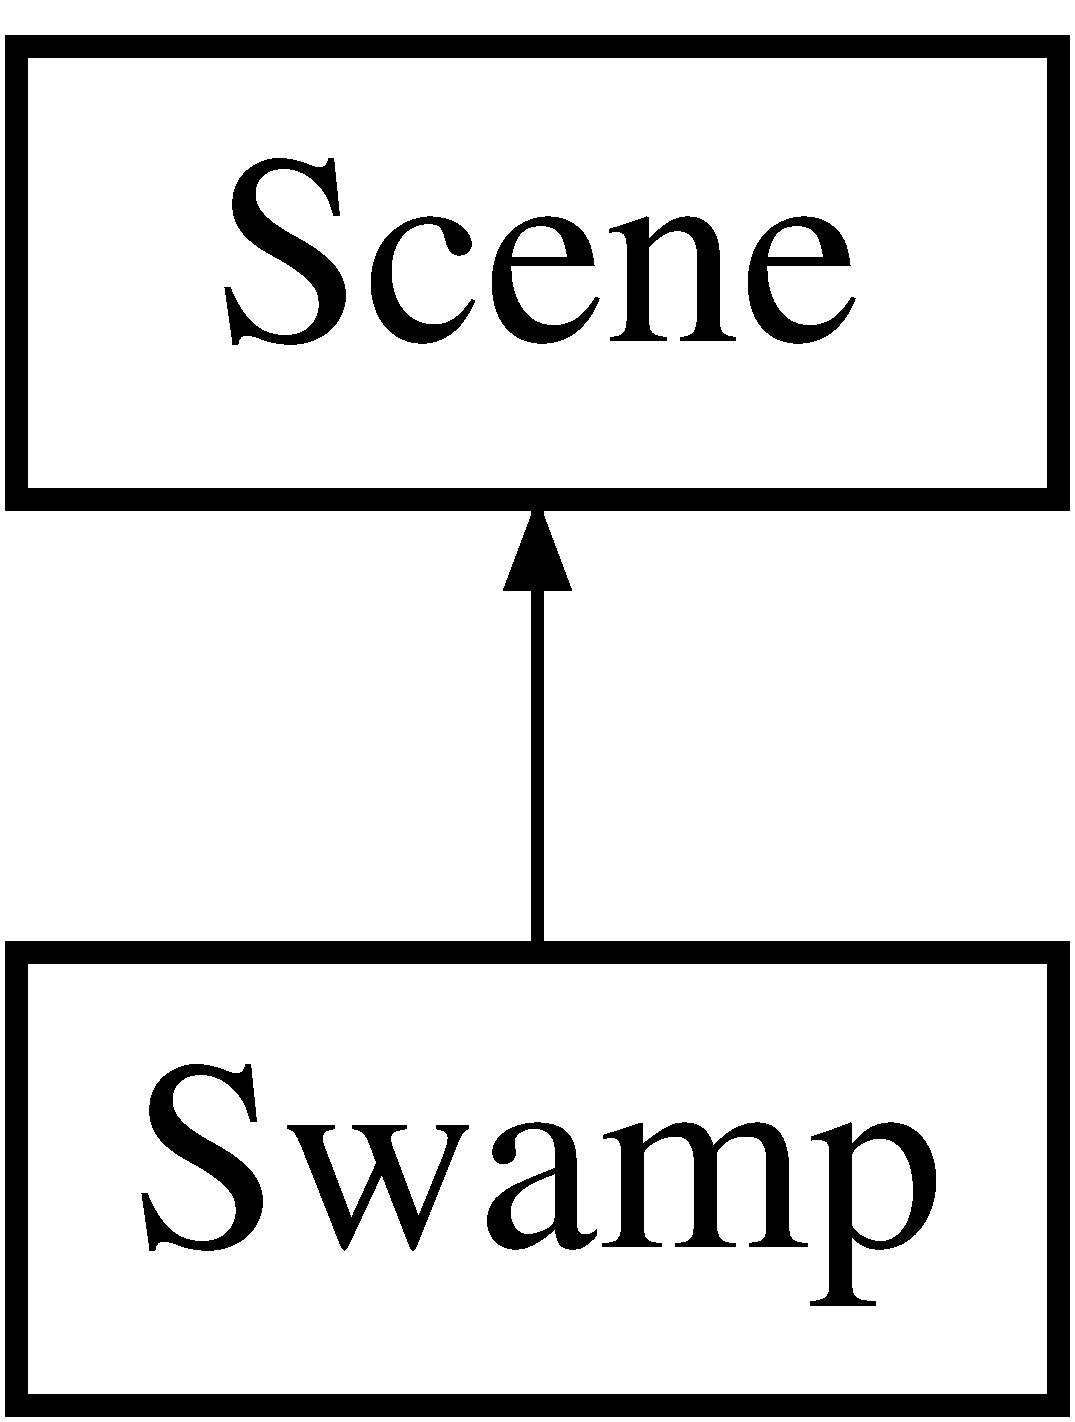
\includegraphics[height=2.000000cm]{class_swamp}
\end{center}
\end{figure}
\subsection*{Public Member Functions}
\begin{DoxyCompactItemize}
\item 
\hyperlink{class_swamp_a45f2bf5cac3f361031af5e9fcce305fe}{Swamp} (S\-D\-L\-\_\-\-Renderer $\ast$\-\_\-renderer)
\item 
\hyperlink{class_swamp_a5de2deafe21f3af8c721b10dca815dfe}{$\sim$\-Swamp} (void)
\item 
void \hyperlink{class_swamp_a0e6d0b3c4d33ac5fe9dca413fd0be908}{Draw} ()
\item 
void \hyperlink{class_swamp_a3df7416f9f5e3a022c53981476001a7d}{Update} ()
\end{DoxyCompactItemize}


\subsection{Constructor \& Destructor Documentation}
\hypertarget{class_swamp_a45f2bf5cac3f361031af5e9fcce305fe}{\index{Swamp@{Swamp}!Swamp@{Swamp}}
\index{Swamp@{Swamp}!Swamp@{Swamp}}
\subsubsection[{Swamp}]{\setlength{\rightskip}{0pt plus 5cm}Swamp\-::\-Swamp (
\begin{DoxyParamCaption}
\item[{S\-D\-L\-\_\-\-Renderer $\ast$}]{\-\_\-renderer}
\end{DoxyParamCaption}
)}}\label{class_swamp_a45f2bf5cac3f361031af5e9fcce305fe}
\hypertarget{class_swamp_a5de2deafe21f3af8c721b10dca815dfe}{\index{Swamp@{Swamp}!$\sim$\-Swamp@{$\sim$\-Swamp}}
\index{$\sim$\-Swamp@{$\sim$\-Swamp}!Swamp@{Swamp}}
\subsubsection[{$\sim$\-Swamp}]{\setlength{\rightskip}{0pt plus 5cm}Swamp\-::$\sim$\-Swamp (
\begin{DoxyParamCaption}
\item[{void}]{}
\end{DoxyParamCaption}
)}}\label{class_swamp_a5de2deafe21f3af8c721b10dca815dfe}


\subsection{Member Function Documentation}
\hypertarget{class_swamp_a0e6d0b3c4d33ac5fe9dca413fd0be908}{\index{Swamp@{Swamp}!Draw@{Draw}}
\index{Draw@{Draw}!Swamp@{Swamp}}
\subsubsection[{Draw}]{\setlength{\rightskip}{0pt plus 5cm}void Swamp\-::\-Draw (
\begin{DoxyParamCaption}
{}
\end{DoxyParamCaption}
)}}\label{class_swamp_a0e6d0b3c4d33ac5fe9dca413fd0be908}
\hypertarget{class_swamp_a3df7416f9f5e3a022c53981476001a7d}{\index{Swamp@{Swamp}!Update@{Update}}
\index{Update@{Update}!Swamp@{Swamp}}
\subsubsection[{Update}]{\setlength{\rightskip}{0pt plus 5cm}void Swamp\-::\-Update (
\begin{DoxyParamCaption}
{}
\end{DoxyParamCaption}
)}}\label{class_swamp_a3df7416f9f5e3a022c53981476001a7d}


The documentation for this class was generated from the following file\-:\begin{DoxyCompactItemize}
\item 
Joes\-\_\-\-S\-D\-L\-\_\-\-Framework/\hyperlink{_swamp_8h}{Swamp.\-h}\end{DoxyCompactItemize}

\hypertarget{class_variable_terrain}{\section{Variable\-Terrain Class Reference}
\label{class_variable_terrain}\index{Variable\-Terrain@{Variable\-Terrain}}
}


{\ttfamily \#include $<$Variable\-Terrain.\-h$>$}

Inheritance diagram for Variable\-Terrain\-:\begin{figure}[H]
\begin{center}
\leavevmode
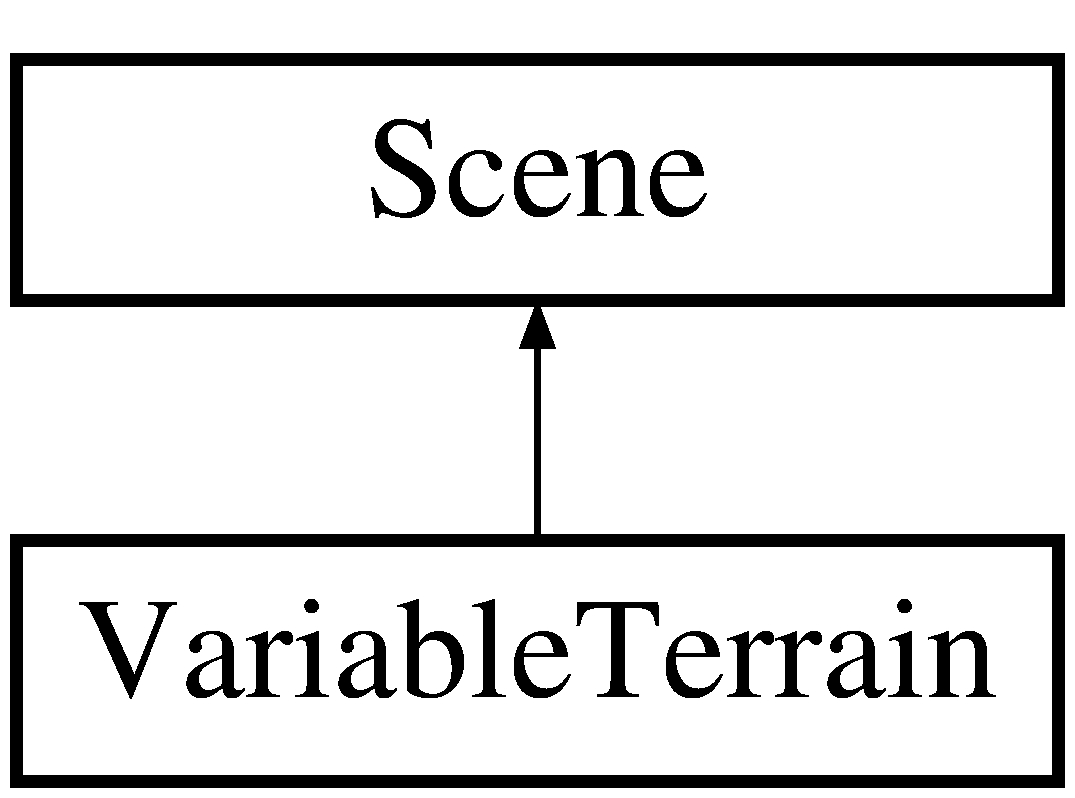
\includegraphics[height=2.000000cm]{class_variable_terrain}
\end{center}
\end{figure}
\subsection*{Public Member Functions}
\begin{DoxyCompactItemize}
\item 
\hyperlink{class_variable_terrain_a114ca86308369f464e63fc03560caa9e}{Variable\-Terrain} (S\-D\-L\-\_\-\-Renderer $\ast$\-\_\-renderer)
\item 
\hyperlink{class_variable_terrain_a27c1ebdc6c0fe991d4ec9cced5de5814}{$\sim$\-Variable\-Terrain} (void)
\item 
void \hyperlink{class_variable_terrain_adf2c137673e2888d603e361368a83467}{Draw} ()
\item 
void \hyperlink{class_variable_terrain_a5084bbc51d4528c20f4b369a342ab0ee}{Update} ()
\end{DoxyCompactItemize}


\subsection{Constructor \& Destructor Documentation}
\hypertarget{class_variable_terrain_a114ca86308369f464e63fc03560caa9e}{\index{Variable\-Terrain@{Variable\-Terrain}!Variable\-Terrain@{Variable\-Terrain}}
\index{Variable\-Terrain@{Variable\-Terrain}!VariableTerrain@{Variable\-Terrain}}
\subsubsection[{Variable\-Terrain}]{\setlength{\rightskip}{0pt plus 5cm}Variable\-Terrain\-::\-Variable\-Terrain (
\begin{DoxyParamCaption}
\item[{S\-D\-L\-\_\-\-Renderer $\ast$}]{\-\_\-renderer}
\end{DoxyParamCaption}
)}}\label{class_variable_terrain_a114ca86308369f464e63fc03560caa9e}
\hypertarget{class_variable_terrain_a27c1ebdc6c0fe991d4ec9cced5de5814}{\index{Variable\-Terrain@{Variable\-Terrain}!$\sim$\-Variable\-Terrain@{$\sim$\-Variable\-Terrain}}
\index{$\sim$\-Variable\-Terrain@{$\sim$\-Variable\-Terrain}!VariableTerrain@{Variable\-Terrain}}
\subsubsection[{$\sim$\-Variable\-Terrain}]{\setlength{\rightskip}{0pt plus 5cm}Variable\-Terrain\-::$\sim$\-Variable\-Terrain (
\begin{DoxyParamCaption}
\item[{void}]{}
\end{DoxyParamCaption}
)}}\label{class_variable_terrain_a27c1ebdc6c0fe991d4ec9cced5de5814}


\subsection{Member Function Documentation}
\hypertarget{class_variable_terrain_adf2c137673e2888d603e361368a83467}{\index{Variable\-Terrain@{Variable\-Terrain}!Draw@{Draw}}
\index{Draw@{Draw}!VariableTerrain@{Variable\-Terrain}}
\subsubsection[{Draw}]{\setlength{\rightskip}{0pt plus 5cm}void Variable\-Terrain\-::\-Draw (
\begin{DoxyParamCaption}
{}
\end{DoxyParamCaption}
)}}\label{class_variable_terrain_adf2c137673e2888d603e361368a83467}
\hypertarget{class_variable_terrain_a5084bbc51d4528c20f4b369a342ab0ee}{\index{Variable\-Terrain@{Variable\-Terrain}!Update@{Update}}
\index{Update@{Update}!VariableTerrain@{Variable\-Terrain}}
\subsubsection[{Update}]{\setlength{\rightskip}{0pt plus 5cm}void Variable\-Terrain\-::\-Update (
\begin{DoxyParamCaption}
{}
\end{DoxyParamCaption}
)}}\label{class_variable_terrain_a5084bbc51d4528c20f4b369a342ab0ee}


The documentation for this class was generated from the following file\-:\begin{DoxyCompactItemize}
\item 
Joes\-\_\-\-S\-D\-L\-\_\-\-Framework/\hyperlink{_variable_terrain_8h}{Variable\-Terrain.\-h}\end{DoxyCompactItemize}

\hypertarget{class_x_d_l___camera}{\section{X\-D\-L\-\_\-\-Camera Class Reference}
\label{class_x_d_l___camera}\index{X\-D\-L\-\_\-\-Camera@{X\-D\-L\-\_\-\-Camera}}
}


X\-D\-L\-\_\-\-Camaera. \mbox{[}Singleton\mbox{]}.  




{\ttfamily \#include $<$X\-D\-L\-\_\-\-Camera.\-h$>$}

\subsection*{Public Member Functions}
\begin{DoxyCompactItemize}
\item 
\hyperlink{class_x_d_l___camera_aeca108c3495c9fca85f150932ee77eae}{$\sim$\-X\-D\-L\-\_\-\-Camera} (void)
\item 
void \hyperlink{class_x_d_l___camera_a4a973ddf2f7ab261f8bbaec4a911ba5e}{Set\-Zoom} (float \-\_\-zoom)
\item 
float \hyperlink{class_x_d_l___camera_afb54ec9b1efa5cf23faea192a63d8d44}{Get\-Current\-Zoom} ()
\item 
void \hyperlink{class_x_d_l___camera_a95e3e2c8dbbcaba8d9a6f572f1c0919d}{Set\-Position} (int \-\_\-x, int \-\_\-y)
\item 
S\-D\-L\-\_\-\-Point $\ast$ \hyperlink{class_x_d_l___camera_aaf2329b5bed3bdd0f679f3ce39d7aa89}{Get\-Position} ()
\end{DoxyCompactItemize}
\subsection*{Static Public Member Functions}
\begin{DoxyCompactItemize}
\item 
static \hyperlink{class_x_d_l___camera}{X\-D\-L\-\_\-\-Camera} $\ast$ \hyperlink{class_x_d_l___camera_af972e4ad4d82db12161f0b3c0234f279}{Get\-Instance} ()
\end{DoxyCompactItemize}


\subsection{Detailed Description}
X\-D\-L\-\_\-\-Camaera. \mbox{[}Singleton\mbox{]}. 

Not technically a camera, but a structure to control the scale and position of our drawing surface. 

\subsection{Constructor \& Destructor Documentation}
\hypertarget{class_x_d_l___camera_aeca108c3495c9fca85f150932ee77eae}{\index{X\-D\-L\-\_\-\-Camera@{X\-D\-L\-\_\-\-Camera}!$\sim$\-X\-D\-L\-\_\-\-Camera@{$\sim$\-X\-D\-L\-\_\-\-Camera}}
\index{$\sim$\-X\-D\-L\-\_\-\-Camera@{$\sim$\-X\-D\-L\-\_\-\-Camera}!XDL_Camera@{X\-D\-L\-\_\-\-Camera}}
\subsubsection[{$\sim$\-X\-D\-L\-\_\-\-Camera}]{\setlength{\rightskip}{0pt plus 5cm}X\-D\-L\-\_\-\-Camera\-::$\sim$\-X\-D\-L\-\_\-\-Camera (
\begin{DoxyParamCaption}
\item[{void}]{}
\end{DoxyParamCaption}
)}}\label{class_x_d_l___camera_aeca108c3495c9fca85f150932ee77eae}


\subsection{Member Function Documentation}
\hypertarget{class_x_d_l___camera_afb54ec9b1efa5cf23faea192a63d8d44}{\index{X\-D\-L\-\_\-\-Camera@{X\-D\-L\-\_\-\-Camera}!Get\-Current\-Zoom@{Get\-Current\-Zoom}}
\index{Get\-Current\-Zoom@{Get\-Current\-Zoom}!XDL_Camera@{X\-D\-L\-\_\-\-Camera}}
\subsubsection[{Get\-Current\-Zoom}]{\setlength{\rightskip}{0pt plus 5cm}float X\-D\-L\-\_\-\-Camera\-::\-Get\-Current\-Zoom (
\begin{DoxyParamCaption}
{}
\end{DoxyParamCaption}
)}}\label{class_x_d_l___camera_afb54ec9b1efa5cf23faea192a63d8d44}

\begin{DoxyParams}{Parameters}
{\em \-\_\-zoom} & Zoom level, set it to 1 as default.\\
\hline
\end{DoxyParams}
\begin{DoxyReturn}{Returns}
current Zoom level as a float.\-Getter for Zoom 
\end{DoxyReturn}
\hypertarget{class_x_d_l___camera_af972e4ad4d82db12161f0b3c0234f279}{\index{X\-D\-L\-\_\-\-Camera@{X\-D\-L\-\_\-\-Camera}!Get\-Instance@{Get\-Instance}}
\index{Get\-Instance@{Get\-Instance}!XDL_Camera@{X\-D\-L\-\_\-\-Camera}}
\subsubsection[{Get\-Instance}]{\setlength{\rightskip}{0pt plus 5cm}{\bf X\-D\-L\-\_\-\-Camera} $\ast$ X\-D\-L\-\_\-\-Camera\-::\-Get\-Instance (
\begin{DoxyParamCaption}
{}
\end{DoxyParamCaption}
)\hspace{0.3cm}{\ttfamily [static]}}}\label{class_x_d_l___camera_af972e4ad4d82db12161f0b3c0234f279}
\begin{DoxyReturn}{Returns}
pointer to the camera instance.\-Creates one if none exists\mbox{[}Lazy\-Loading\mbox{]}Get Instance, which will return a pointer to our camera 
\end{DoxyReturn}
\hypertarget{class_x_d_l___camera_aaf2329b5bed3bdd0f679f3ce39d7aa89}{\index{X\-D\-L\-\_\-\-Camera@{X\-D\-L\-\_\-\-Camera}!Get\-Position@{Get\-Position}}
\index{Get\-Position@{Get\-Position}!XDL_Camera@{X\-D\-L\-\_\-\-Camera}}
\subsubsection[{Get\-Position}]{\setlength{\rightskip}{0pt plus 5cm}S\-D\-L\-\_\-\-Point $\ast$ X\-D\-L\-\_\-\-Camera\-::\-Get\-Position (
\begin{DoxyParamCaption}
{}
\end{DoxyParamCaption}
)}}\label{class_x_d_l___camera_aaf2329b5bed3bdd0f679f3ce39d7aa89}
\begin{DoxyReturn}{Returns}
pointer to an S\-D\-L\-\_\-\-Point, which contains the X and Y position of the world.\-Getter for position 
\end{DoxyReturn}
\hypertarget{class_x_d_l___camera_a95e3e2c8dbbcaba8d9a6f572f1c0919d}{\index{X\-D\-L\-\_\-\-Camera@{X\-D\-L\-\_\-\-Camera}!Set\-Position@{Set\-Position}}
\index{Set\-Position@{Set\-Position}!XDL_Camera@{X\-D\-L\-\_\-\-Camera}}
\subsubsection[{Set\-Position}]{\setlength{\rightskip}{0pt plus 5cm}void X\-D\-L\-\_\-\-Camera\-::\-Set\-Position (
\begin{DoxyParamCaption}
\item[{int}]{\-\_\-x, }
\item[{int}]{\-\_\-y}
\end{DoxyParamCaption}
)}}\label{class_x_d_l___camera_a95e3e2c8dbbcaba8d9a6f572f1c0919d}

\begin{DoxyParams}{Parameters}
{\em \-\_\-x} & X position of the world. \\
\hline
{\em \-\_\-y} & Y position of the world.\-Set the worlds position relative to the window. By default its (0,0), which means anything left/above of the screen will never be drawn. Because of this, it might not be a bad idea to move it \\
\hline
\end{DoxyParams}
\hypertarget{class_x_d_l___camera_a4a973ddf2f7ab261f8bbaec4a911ba5e}{\index{X\-D\-L\-\_\-\-Camera@{X\-D\-L\-\_\-\-Camera}!Set\-Zoom@{Set\-Zoom}}
\index{Set\-Zoom@{Set\-Zoom}!XDL_Camera@{X\-D\-L\-\_\-\-Camera}}
\subsubsection[{Set\-Zoom}]{\setlength{\rightskip}{0pt plus 5cm}void X\-D\-L\-\_\-\-Camera\-::\-Set\-Zoom (
\begin{DoxyParamCaption}
\item[{float}]{\-\_\-zoom}
\end{DoxyParamCaption}
)}}\label{class_x_d_l___camera_a4a973ddf2f7ab261f8bbaec4a911ba5e}

\begin{DoxyParams}{Parameters}
{\em \-\_\-zoom} & Zoom level, set it to 1 as default.\-Sets the zoom of our world, in reality, it sets the scale of our drawing surface, after all drawing has occurred \\
\hline
\end{DoxyParams}


The documentation for this class was generated from the following files\-:\begin{DoxyCompactItemize}
\item 
Joes\-\_\-\-S\-D\-L\-\_\-\-Framework/\hyperlink{_x_d_l___camera_8h}{X\-D\-L\-\_\-\-Camera.\-h}\item 
Joes\-\_\-\-S\-D\-L\-\_\-\-Framework/\hyperlink{_x_d_l___camera_8cpp}{X\-D\-L\-\_\-\-Camera.\-cpp}\end{DoxyCompactItemize}

\hypertarget{class_x_d_l___content_manager}{\section{X\-D\-L\-\_\-\-Content\-Manager Class Reference}
\label{class_x_d_l___content_manager}\index{X\-D\-L\-\_\-\-Content\-Manager@{X\-D\-L\-\_\-\-Content\-Manager}}
}


{\ttfamily \#include $<$X\-D\-L\-\_\-\-Content\-Manager.\-h$>$}

\subsection*{Public Member Functions}
\begin{DoxyCompactItemize}
\item 
\hyperlink{class_x_d_l___content_manager_af04e583d32143b502cb060261159853d}{X\-D\-L\-\_\-\-Content\-Manager} (void)
\item 
\hyperlink{class_x_d_l___content_manager_a2d7112bce7c871270e070e4c69179e3b}{$\sim$\-X\-D\-L\-\_\-\-Content\-Manager} (void)
\item 
S\-D\-L\-\_\-\-Texture $\ast$ \hyperlink{class_x_d_l___content_manager_a99571fb38d9673ede5cd8598b3081f11}{Load\-B\-M\-P} (char $\ast$\-\_\-path, S\-D\-L\-\_\-\-Renderer $\ast$\-\_\-renderer)
\item 
S\-D\-L\-\_\-\-Texture $\ast$ \hyperlink{class_x_d_l___content_manager_a833df37fbdf51abe274454f4cfee1d0c}{Load\-Sprite} (char $\ast$\-\_\-path, S\-D\-L\-\_\-\-Renderer $\ast$\-\_\-renderer)
\begin{DoxyCompactList}\small\item\em Load\-Sprite. \end{DoxyCompactList}\end{DoxyCompactItemize}
\subsection*{Static Public Member Functions}
\begin{DoxyCompactItemize}
\item 
static \hyperlink{class_x_d_l___content_manager}{X\-D\-L\-\_\-\-Content\-Manager} $\ast$ \hyperlink{class_x_d_l___content_manager_ab1ce9134a3c5a21f8372b0224559cb81}{Get\-Instance} ()
\end{DoxyCompactItemize}


\subsection{Constructor \& Destructor Documentation}
\hypertarget{class_x_d_l___content_manager_af04e583d32143b502cb060261159853d}{\index{X\-D\-L\-\_\-\-Content\-Manager@{X\-D\-L\-\_\-\-Content\-Manager}!X\-D\-L\-\_\-\-Content\-Manager@{X\-D\-L\-\_\-\-Content\-Manager}}
\index{X\-D\-L\-\_\-\-Content\-Manager@{X\-D\-L\-\_\-\-Content\-Manager}!XDL_ContentManager@{X\-D\-L\-\_\-\-Content\-Manager}}
\subsubsection[{X\-D\-L\-\_\-\-Content\-Manager}]{\setlength{\rightskip}{0pt plus 5cm}X\-D\-L\-\_\-\-Content\-Manager\-::\-X\-D\-L\-\_\-\-Content\-Manager (
\begin{DoxyParamCaption}
\item[{void}]{}
\end{DoxyParamCaption}
)}}\label{class_x_d_l___content_manager_af04e583d32143b502cb060261159853d}
\hypertarget{class_x_d_l___content_manager_a2d7112bce7c871270e070e4c69179e3b}{\index{X\-D\-L\-\_\-\-Content\-Manager@{X\-D\-L\-\_\-\-Content\-Manager}!$\sim$\-X\-D\-L\-\_\-\-Content\-Manager@{$\sim$\-X\-D\-L\-\_\-\-Content\-Manager}}
\index{$\sim$\-X\-D\-L\-\_\-\-Content\-Manager@{$\sim$\-X\-D\-L\-\_\-\-Content\-Manager}!XDL_ContentManager@{X\-D\-L\-\_\-\-Content\-Manager}}
\subsubsection[{$\sim$\-X\-D\-L\-\_\-\-Content\-Manager}]{\setlength{\rightskip}{0pt plus 5cm}X\-D\-L\-\_\-\-Content\-Manager\-::$\sim$\-X\-D\-L\-\_\-\-Content\-Manager (
\begin{DoxyParamCaption}
\item[{void}]{}
\end{DoxyParamCaption}
)}}\label{class_x_d_l___content_manager_a2d7112bce7c871270e070e4c69179e3b}


\subsection{Member Function Documentation}
\hypertarget{class_x_d_l___content_manager_ab1ce9134a3c5a21f8372b0224559cb81}{\index{X\-D\-L\-\_\-\-Content\-Manager@{X\-D\-L\-\_\-\-Content\-Manager}!Get\-Instance@{Get\-Instance}}
\index{Get\-Instance@{Get\-Instance}!XDL_ContentManager@{X\-D\-L\-\_\-\-Content\-Manager}}
\subsubsection[{Get\-Instance}]{\setlength{\rightskip}{0pt plus 5cm}{\bf X\-D\-L\-\_\-\-Content\-Manager} $\ast$ X\-D\-L\-\_\-\-Content\-Manager\-::\-Get\-Instance (
\begin{DoxyParamCaption}
{}
\end{DoxyParamCaption}
)\hspace{0.3cm}{\ttfamily [static]}}}\label{class_x_d_l___content_manager_ab1ce9134a3c5a21f8372b0224559cb81}
\begin{DoxyReturn}{Returns}
Pointer to \hyperlink{class_x_d_l___content_manager}{X\-D\-L\-\_\-\-Content\-Manager} Instance.\-Creates a new Content\-Manager if none exist.\-Depricated 
\end{DoxyReturn}
\hypertarget{class_x_d_l___content_manager_a99571fb38d9673ede5cd8598b3081f11}{\index{X\-D\-L\-\_\-\-Content\-Manager@{X\-D\-L\-\_\-\-Content\-Manager}!Load\-B\-M\-P@{Load\-B\-M\-P}}
\index{Load\-B\-M\-P@{Load\-B\-M\-P}!XDL_ContentManager@{X\-D\-L\-\_\-\-Content\-Manager}}
\subsubsection[{Load\-B\-M\-P}]{\setlength{\rightskip}{0pt plus 5cm}S\-D\-L\-\_\-\-Texture$\ast$ X\-D\-L\-\_\-\-Content\-Manager\-::\-Load\-B\-M\-P (
\begin{DoxyParamCaption}
\item[{char $\ast$}]{\-\_\-path, }
\item[{S\-D\-L\-\_\-\-Renderer $\ast$}]{\-\_\-renderer}
\end{DoxyParamCaption}
)}}\label{class_x_d_l___content_manager_a99571fb38d9673ede5cd8598b3081f11}
\begin{DoxySeeAlso}{See Also}
\hyperlink{class_x_d_l___content_manager_a833df37fbdf51abe274454f4cfee1d0c}{Load\-Sprite(char$\ast$ \-\_\-path,\-S\-D\-L\-\_\-\-Renderer$\ast$ \-\_\-renderer)} 
\end{DoxySeeAlso}
\hypertarget{class_x_d_l___content_manager_a833df37fbdf51abe274454f4cfee1d0c}{\index{X\-D\-L\-\_\-\-Content\-Manager@{X\-D\-L\-\_\-\-Content\-Manager}!Load\-Sprite@{Load\-Sprite}}
\index{Load\-Sprite@{Load\-Sprite}!XDL_ContentManager@{X\-D\-L\-\_\-\-Content\-Manager}}
\subsubsection[{Load\-Sprite}]{\setlength{\rightskip}{0pt plus 5cm}S\-D\-L\-\_\-\-Texture $\ast$ X\-D\-L\-\_\-\-Content\-Manager\-::\-Load\-Sprite (
\begin{DoxyParamCaption}
\item[{char $\ast$}]{\-\_\-path, }
\item[{S\-D\-L\-\_\-\-Renderer $\ast$}]{\-\_\-renderer}
\end{DoxyParamCaption}
)}}\label{class_x_d_l___content_manager_a833df37fbdf51abe274454f4cfee1d0c}


Load\-Sprite. 

\begin{DoxyReturn}{Returns}
Pointer to an S\-D\-L\-\_\-\-Texture holding our sprite 
\end{DoxyReturn}

\begin{DoxyParams}{Parameters}
{\em \-\_\-path} & Path to the sprite \\
\hline
{\em \-\_\-renderer} & Pointer to the current draw surface\\
\hline
\end{DoxyParams}
Loads a sprite into memory.\-If it is already in memory, it will return a pointer to the loaded asset.\-If its the first time loading, it will store it in a map for future use. 

The documentation for this class was generated from the following files\-:\begin{DoxyCompactItemize}
\item 
Joes\-\_\-\-S\-D\-L\-\_\-\-Framework/\hyperlink{_x_d_l___content_manager_8h}{X\-D\-L\-\_\-\-Content\-Manager.\-h}\item 
Joes\-\_\-\-S\-D\-L\-\_\-\-Framework/\hyperlink{_x_d_l___content_manager_8cpp}{X\-D\-L\-\_\-\-Content\-Manager.\-cpp}\end{DoxyCompactItemize}

\hypertarget{class_x_d_l___game}{\section{X\-D\-L\-\_\-\-Game Class Reference}
\label{class_x_d_l___game}\index{X\-D\-L\-\_\-\-Game@{X\-D\-L\-\_\-\-Game}}
}


\hyperlink{class_x_d_l___game}{X\-D\-L\-\_\-\-Game}.  




{\ttfamily \#include $<$X\-D\-L\-\_\-\-Game.\-h$>$}

\subsection*{Public Member Functions}
\begin{DoxyCompactItemize}
\item 
\hyperlink{class_x_d_l___game_a7dbac78db43464ec6abf72cc0b83798c}{X\-D\-L\-\_\-\-Game} (void)
\item 
\hyperlink{class_x_d_l___game_ae74cceb6cbe74cdaefcc0c69ad0e88f2}{$\sim$\-X\-D\-L\-\_\-\-Game} (void)
\item 
bool \hyperlink{class_x_d_l___game_ab866479bed0d2d4ab2d8c40b8d2b1206}{Init} ()
\item 
void \hyperlink{class_x_d_l___game_afca16922cbee9332ac6b8fabf8078c4d}{Update} ()
\item 
void \hyperlink{class_x_d_l___game_a8259b7f7bc74722f423e0392cebef188}{Render} ()
\item 
void \hyperlink{class_x_d_l___game_a03405ef0205b25414b86d833cb4cd562}{Clean\-Up} ()
\end{DoxyCompactItemize}
\subsection*{Public Attributes}
\begin{DoxyCompactItemize}
\item 
S\-D\-L\-\_\-\-Renderer $\ast$ \hyperlink{class_x_d_l___game_a64e272606ee7d43ab1669794c098c2c4}{\-\_\-renderer}
\end{DoxyCompactItemize}
\subsection*{Static Public Attributes}
\begin{DoxyCompactItemize}
\item 
static int \hyperlink{class_x_d_l___game_a2168cd95816117ff5f905692439aeb72}{S\-C\-R\-E\-E\-N\-\_\-\-W\-I\-D\-T\-H}
\item 
static int \hyperlink{class_x_d_l___game_a9fde7fa33a7816a1e3f17313ebca9001}{S\-C\-R\-E\-E\-N\-\_\-\-H\-E\-I\-G\-H\-T}
\item 
static int \hyperlink{class_x_d_l___game_a0c6b24dee1668f4a1079d389efda2ccf}{\-\_\-r}
\item 
static int \hyperlink{class_x_d_l___game_a0d18c646bd050e6e5bf93efd1b00a8a8}{\-\_\-g}
\item 
static int \hyperlink{class_x_d_l___game_a2d89ed8221d33e4a4351c93d4190464c}{\-\_\-b}
\item 
static S\-D\-L\-\_\-\-Rect $\ast$ \hyperlink{class_x_d_l___game_aba18e8d33ee6e87494ebb958f2beee67}{\-\_\-windows\-Bounds}
\end{DoxyCompactItemize}


\subsection{Detailed Description}
\hyperlink{class_x_d_l___game}{X\-D\-L\-\_\-\-Game}. 

Sets up S\-D\-L and our game loop. 

\subsection{Constructor \& Destructor Documentation}
\hypertarget{class_x_d_l___game_a7dbac78db43464ec6abf72cc0b83798c}{\index{X\-D\-L\-\_\-\-Game@{X\-D\-L\-\_\-\-Game}!X\-D\-L\-\_\-\-Game@{X\-D\-L\-\_\-\-Game}}
\index{X\-D\-L\-\_\-\-Game@{X\-D\-L\-\_\-\-Game}!XDL_Game@{X\-D\-L\-\_\-\-Game}}
\subsubsection[{X\-D\-L\-\_\-\-Game}]{\setlength{\rightskip}{0pt plus 5cm}X\-D\-L\-\_\-\-Game\-::\-X\-D\-L\-\_\-\-Game (
\begin{DoxyParamCaption}
\item[{void}]{}
\end{DoxyParamCaption}
)}}\label{class_x_d_l___game_a7dbac78db43464ec6abf72cc0b83798c}
\hypertarget{class_x_d_l___game_ae74cceb6cbe74cdaefcc0c69ad0e88f2}{\index{X\-D\-L\-\_\-\-Game@{X\-D\-L\-\_\-\-Game}!$\sim$\-X\-D\-L\-\_\-\-Game@{$\sim$\-X\-D\-L\-\_\-\-Game}}
\index{$\sim$\-X\-D\-L\-\_\-\-Game@{$\sim$\-X\-D\-L\-\_\-\-Game}!XDL_Game@{X\-D\-L\-\_\-\-Game}}
\subsubsection[{$\sim$\-X\-D\-L\-\_\-\-Game}]{\setlength{\rightskip}{0pt plus 5cm}X\-D\-L\-\_\-\-Game\-::$\sim$\-X\-D\-L\-\_\-\-Game (
\begin{DoxyParamCaption}
\item[{void}]{}
\end{DoxyParamCaption}
)}}\label{class_x_d_l___game_ae74cceb6cbe74cdaefcc0c69ad0e88f2}


\subsection{Member Function Documentation}
\hypertarget{class_x_d_l___game_a03405ef0205b25414b86d833cb4cd562}{\index{X\-D\-L\-\_\-\-Game@{X\-D\-L\-\_\-\-Game}!Clean\-Up@{Clean\-Up}}
\index{Clean\-Up@{Clean\-Up}!XDL_Game@{X\-D\-L\-\_\-\-Game}}
\subsubsection[{Clean\-Up}]{\setlength{\rightskip}{0pt plus 5cm}void X\-D\-L\-\_\-\-Game\-::\-Clean\-Up (
\begin{DoxyParamCaption}
{}
\end{DoxyParamCaption}
)}}\label{class_x_d_l___game_a03405ef0205b25414b86d833cb4cd562}
Cleans up S\-D\-L when game exits \hypertarget{class_x_d_l___game_ab866479bed0d2d4ab2d8c40b8d2b1206}{\index{X\-D\-L\-\_\-\-Game@{X\-D\-L\-\_\-\-Game}!Init@{Init}}
\index{Init@{Init}!XDL_Game@{X\-D\-L\-\_\-\-Game}}
\subsubsection[{Init}]{\setlength{\rightskip}{0pt plus 5cm}bool X\-D\-L\-\_\-\-Game\-::\-Init (
\begin{DoxyParamCaption}
{}
\end{DoxyParamCaption}
)}}\label{class_x_d_l___game_ab866479bed0d2d4ab2d8c40b8d2b1206}
Sets up our window, initializes S\-D\-L and our Scene\-Manager to navigate scenes \hypertarget{class_x_d_l___game_a8259b7f7bc74722f423e0392cebef188}{\index{X\-D\-L\-\_\-\-Game@{X\-D\-L\-\_\-\-Game}!Render@{Render}}
\index{Render@{Render}!XDL_Game@{X\-D\-L\-\_\-\-Game}}
\subsubsection[{Render}]{\setlength{\rightskip}{0pt plus 5cm}void X\-D\-L\-\_\-\-Game\-::\-Render (
\begin{DoxyParamCaption}
{}
\end{DoxyParamCaption}
)}}\label{class_x_d_l___game_a8259b7f7bc74722f423e0392cebef188}
Called every frame (60 times a second). Calls Scene\-Managers Draw, which in turn leverages \hyperlink{class_x_d_l___sprite_batch}{X\-D\-L\-\_\-\-Sprite\-Batch} to draw our Scene \hypertarget{class_x_d_l___game_afca16922cbee9332ac6b8fabf8078c4d}{\index{X\-D\-L\-\_\-\-Game@{X\-D\-L\-\_\-\-Game}!Update@{Update}}
\index{Update@{Update}!XDL_Game@{X\-D\-L\-\_\-\-Game}}
\subsubsection[{Update}]{\setlength{\rightskip}{0pt plus 5cm}void X\-D\-L\-\_\-\-Game\-::\-Update (
\begin{DoxyParamCaption}
{}
\end{DoxyParamCaption}
)}}\label{class_x_d_l___game_afca16922cbee9332ac6b8fabf8078c4d}
Called every frame (60 times a second). Basically calls Scene\-Managers Update, which in turn updates the current Scene 

\subsection{Member Data Documentation}
\hypertarget{class_x_d_l___game_a2d89ed8221d33e4a4351c93d4190464c}{\index{X\-D\-L\-\_\-\-Game@{X\-D\-L\-\_\-\-Game}!\-\_\-b@{\-\_\-b}}
\index{\-\_\-b@{\-\_\-b}!XDL_Game@{X\-D\-L\-\_\-\-Game}}
\subsubsection[{\-\_\-b}]{\setlength{\rightskip}{0pt plus 5cm}int X\-D\-L\-\_\-\-Game\-::\-\_\-b\hspace{0.3cm}{\ttfamily [static]}}}\label{class_x_d_l___game_a2d89ed8221d33e4a4351c93d4190464c}
background color \-: Blue (0 -\/255) \hypertarget{class_x_d_l___game_a0d18c646bd050e6e5bf93efd1b00a8a8}{\index{X\-D\-L\-\_\-\-Game@{X\-D\-L\-\_\-\-Game}!\-\_\-g@{\-\_\-g}}
\index{\-\_\-g@{\-\_\-g}!XDL_Game@{X\-D\-L\-\_\-\-Game}}
\subsubsection[{\-\_\-g}]{\setlength{\rightskip}{0pt plus 5cm}int X\-D\-L\-\_\-\-Game\-::\-\_\-g\hspace{0.3cm}{\ttfamily [static]}}}\label{class_x_d_l___game_a0d18c646bd050e6e5bf93efd1b00a8a8}
background color \-: Green (0 -\/255) \hypertarget{class_x_d_l___game_a0c6b24dee1668f4a1079d389efda2ccf}{\index{X\-D\-L\-\_\-\-Game@{X\-D\-L\-\_\-\-Game}!\-\_\-r@{\-\_\-r}}
\index{\-\_\-r@{\-\_\-r}!XDL_Game@{X\-D\-L\-\_\-\-Game}}
\subsubsection[{\-\_\-r}]{\setlength{\rightskip}{0pt plus 5cm}int X\-D\-L\-\_\-\-Game\-::\-\_\-r\hspace{0.3cm}{\ttfamily [static]}}}\label{class_x_d_l___game_a0c6b24dee1668f4a1079d389efda2ccf}
background color \-: Red (0 -\/255) \hypertarget{class_x_d_l___game_a64e272606ee7d43ab1669794c098c2c4}{\index{X\-D\-L\-\_\-\-Game@{X\-D\-L\-\_\-\-Game}!\-\_\-renderer@{\-\_\-renderer}}
\index{\-\_\-renderer@{\-\_\-renderer}!XDL_Game@{X\-D\-L\-\_\-\-Game}}
\subsubsection[{\-\_\-renderer}]{\setlength{\rightskip}{0pt plus 5cm}S\-D\-L\-\_\-\-Renderer$\ast$ X\-D\-L\-\_\-\-Game\-::\-\_\-renderer}}\label{class_x_d_l___game_a64e272606ee7d43ab1669794c098c2c4}
Our Drawing surface \hypertarget{class_x_d_l___game_aba18e8d33ee6e87494ebb958f2beee67}{\index{X\-D\-L\-\_\-\-Game@{X\-D\-L\-\_\-\-Game}!\-\_\-windows\-Bounds@{\-\_\-windows\-Bounds}}
\index{\-\_\-windows\-Bounds@{\-\_\-windows\-Bounds}!XDL_Game@{X\-D\-L\-\_\-\-Game}}
\subsubsection[{\-\_\-windows\-Bounds}]{\setlength{\rightskip}{0pt plus 5cm}S\-D\-L\-\_\-\-Rect $\ast$ X\-D\-L\-\_\-\-Game\-::\-\_\-windows\-Bounds\hspace{0.3cm}{\ttfamily [static]}}}\label{class_x_d_l___game_aba18e8d33ee6e87494ebb958f2beee67}
S\-D\-L\-\_\-\-Rect to represent the screenbounds \hypertarget{class_x_d_l___game_a9fde7fa33a7816a1e3f17313ebca9001}{\index{X\-D\-L\-\_\-\-Game@{X\-D\-L\-\_\-\-Game}!S\-C\-R\-E\-E\-N\-\_\-\-H\-E\-I\-G\-H\-T@{S\-C\-R\-E\-E\-N\-\_\-\-H\-E\-I\-G\-H\-T}}
\index{S\-C\-R\-E\-E\-N\-\_\-\-H\-E\-I\-G\-H\-T@{S\-C\-R\-E\-E\-N\-\_\-\-H\-E\-I\-G\-H\-T}!XDL_Game@{X\-D\-L\-\_\-\-Game}}
\subsubsection[{S\-C\-R\-E\-E\-N\-\_\-\-H\-E\-I\-G\-H\-T}]{\setlength{\rightskip}{0pt plus 5cm}int X\-D\-L\-\_\-\-Game\-::\-S\-C\-R\-E\-E\-N\-\_\-\-H\-E\-I\-G\-H\-T\hspace{0.3cm}{\ttfamily [static]}}}\label{class_x_d_l___game_a9fde7fa33a7816a1e3f17313ebca9001}
The height of the screen \hypertarget{class_x_d_l___game_a2168cd95816117ff5f905692439aeb72}{\index{X\-D\-L\-\_\-\-Game@{X\-D\-L\-\_\-\-Game}!S\-C\-R\-E\-E\-N\-\_\-\-W\-I\-D\-T\-H@{S\-C\-R\-E\-E\-N\-\_\-\-W\-I\-D\-T\-H}}
\index{S\-C\-R\-E\-E\-N\-\_\-\-W\-I\-D\-T\-H@{S\-C\-R\-E\-E\-N\-\_\-\-W\-I\-D\-T\-H}!XDL_Game@{X\-D\-L\-\_\-\-Game}}
\subsubsection[{S\-C\-R\-E\-E\-N\-\_\-\-W\-I\-D\-T\-H}]{\setlength{\rightskip}{0pt plus 5cm}int X\-D\-L\-\_\-\-Game\-::\-S\-C\-R\-E\-E\-N\-\_\-\-W\-I\-D\-T\-H\hspace{0.3cm}{\ttfamily [static]}}}\label{class_x_d_l___game_a2168cd95816117ff5f905692439aeb72}
The width of the screen 

The documentation for this class was generated from the following files\-:\begin{DoxyCompactItemize}
\item 
Joes\-\_\-\-S\-D\-L\-\_\-\-Framework/\hyperlink{_x_d_l___game_8h}{X\-D\-L\-\_\-\-Game.\-h}\item 
Joes\-\_\-\-S\-D\-L\-\_\-\-Framework/\hyperlink{_x_d_l___game_8cpp}{X\-D\-L\-\_\-\-Game.\-cpp}\end{DoxyCompactItemize}

\hypertarget{class_x_d_l___game_object}{\section{X\-D\-L\-\_\-\-Game\-Object Class Reference}
\label{class_x_d_l___game_object}\index{X\-D\-L\-\_\-\-Game\-Object@{X\-D\-L\-\_\-\-Game\-Object}}
}
Inheritance diagram for X\-D\-L\-\_\-\-Game\-Object\-:\begin{figure}[H]
\begin{center}
\leavevmode
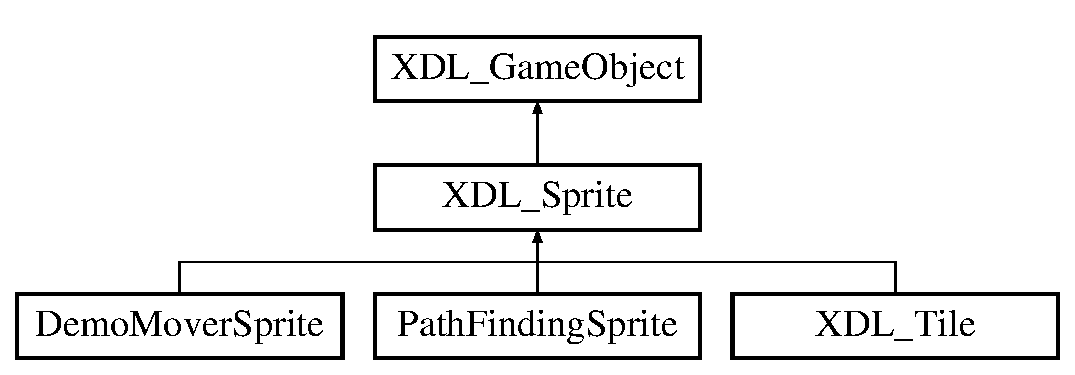
\includegraphics[height=3.000000cm]{class_x_d_l___game_object}
\end{center}
\end{figure}
\subsection*{Public Member Functions}
\begin{DoxyCompactItemize}
\item 
\hypertarget{class_x_d_l___game_object_ac2bf327721f071e6192c5e4691609a98}{{\bfseries X\-D\-L\-\_\-\-Game\-Object} (string \-\_\-name)}\label{class_x_d_l___game_object_ac2bf327721f071e6192c5e4691609a98}

\item 
\hyperlink{class_x_d_l___game_object_a27fd4e872e6e1bb063f5d1c8acf3119c}{$\sim$\-X\-D\-L\-\_\-\-Game\-Object} (void)
\item 
\hypertarget{class_x_d_l___game_object_a65f42bdf8f833262da1b689f9454afd7}{virtual void {\bfseries Init} ()}\label{class_x_d_l___game_object_a65f42bdf8f833262da1b689f9454afd7}

\item 
\hypertarget{class_x_d_l___game_object_a28b5db1a0e150b66e33605d95e6705d5}{virtual void {\bfseries Update} ()}\label{class_x_d_l___game_object_a28b5db1a0e150b66e33605d95e6705d5}

\item 
virtual void \hyperlink{class_x_d_l___game_object_a46ab89c9622631cf13114a493b1b0a2d}{Draw} ()=0
\item 
\hypertarget{class_x_d_l___game_object_ab330c902ae14f980441c95821a4d2652}{void {\bfseries Set\-Velocity} (float \-\_\-x, float \-\_\-y)}\label{class_x_d_l___game_object_ab330c902ae14f980441c95821a4d2652}

\item 
\hypertarget{class_x_d_l___game_object_a0e666a4d38bbe23b32b12f79ea583455}{void {\bfseries Set\-Velocity\-X} (float \-\_\-x)}\label{class_x_d_l___game_object_a0e666a4d38bbe23b32b12f79ea583455}

\item 
\hypertarget{class_x_d_l___game_object_a21374b9d1abd01efdd81dd3fc9b337ee}{void {\bfseries Set\-Velocity\-Y} (float \-\_\-y)}\label{class_x_d_l___game_object_a21374b9d1abd01efdd81dd3fc9b337ee}

\item 
\hypertarget{class_x_d_l___game_object_add121ab40a76ee2189bc4546f4837262}{float {\bfseries Get\-Velocity\-X} ()}\label{class_x_d_l___game_object_add121ab40a76ee2189bc4546f4837262}

\item 
\hypertarget{class_x_d_l___game_object_afb2098323b599609cf87a8e6fe01d10d}{float {\bfseries Get\-Velocity\-Y} ()}\label{class_x_d_l___game_object_afb2098323b599609cf87a8e6fe01d10d}

\item 
\hypertarget{class_x_d_l___game_object_afe3853c83d9b579c29f214ee8f4e973f}{void {\bfseries Set\-Acceleration} (float \-\_\-x, float \-\_\-y)}\label{class_x_d_l___game_object_afe3853c83d9b579c29f214ee8f4e973f}

\item 
\hypertarget{class_x_d_l___game_object_a976621b77d2cd4423bd49588c747a495}{void {\bfseries Set\-Acceleration\-X} (float \-\_\-x)}\label{class_x_d_l___game_object_a976621b77d2cd4423bd49588c747a495}

\item 
\hypertarget{class_x_d_l___game_object_a4eea42378b77c6759b2a9cac4be935f1}{void {\bfseries Set\-Acceleration\-Y} (float \-\_\-y)}\label{class_x_d_l___game_object_a4eea42378b77c6759b2a9cac4be935f1}

\item 
\hypertarget{class_x_d_l___game_object_ace837b938efee5fc0296cdb80b00a683}{float {\bfseries Get\-Acceleration\-X} ()}\label{class_x_d_l___game_object_ace837b938efee5fc0296cdb80b00a683}

\item 
\hypertarget{class_x_d_l___game_object_adfb53693039eaf0f40f61f2679e0c0dd}{float {\bfseries Get\-Acceleration\-Y} ()}\label{class_x_d_l___game_object_adfb53693039eaf0f40f61f2679e0c0dd}

\item 
\hypertarget{class_x_d_l___game_object_a20b8f98a6f5f353b573db1a812088541}{int {\bfseries Get\-Bounds\-X} ()}\label{class_x_d_l___game_object_a20b8f98a6f5f353b573db1a812088541}

\item 
\hypertarget{class_x_d_l___game_object_ad65bdf30e324adc5a4fe03988b787094}{int {\bfseries Get\-Bounds\-Y} ()}\label{class_x_d_l___game_object_ad65bdf30e324adc5a4fe03988b787094}

\item 
\hypertarget{class_x_d_l___game_object_a663d0ad6f06b2341285bc9c63f9ee2dd}{virtual bool {\bfseries Collided\-With} (\hyperlink{class_x_d_l___game_object}{X\-D\-L\-\_\-\-Game\-Object} $\ast$\-\_\-other\-Sprite)}\label{class_x_d_l___game_object_a663d0ad6f06b2341285bc9c63f9ee2dd}

\item 
\hypertarget{class_x_d_l___game_object_a214f85c39378a9c77d6d5cd703718ee4}{virtual bool {\bfseries Overlaps} (S\-D\-L\-\_\-\-Rect \-\_\-sprite, S\-D\-L\-\_\-\-Rect \-\_\-other\-Sprite)}\label{class_x_d_l___game_object_a214f85c39378a9c77d6d5cd703718ee4}

\item 
\hypertarget{class_x_d_l___game_object_ae56fc6434b9e9d5e14b245c1962c8d34}{virtual bool {\bfseries Is\-Touching\-Left} ()}\label{class_x_d_l___game_object_ae56fc6434b9e9d5e14b245c1962c8d34}

\item 
\hypertarget{class_x_d_l___game_object_af75a98fbfa551585b9a8937148bc49b7}{virtual bool {\bfseries Is\-Touching\-Right} ()}\label{class_x_d_l___game_object_af75a98fbfa551585b9a8937148bc49b7}

\item 
\hypertarget{class_x_d_l___game_object_af998b19c3969a60e7bd0ef92e15db2dc}{virtual bool {\bfseries Is\-Touching\-Bottom} ()}\label{class_x_d_l___game_object_af998b19c3969a60e7bd0ef92e15db2dc}

\item 
\hypertarget{class_x_d_l___game_object_a9d15ebd7cac3965a1fe4767e2123f72e}{virtual bool {\bfseries Is\-Touching\-Top} ()}\label{class_x_d_l___game_object_a9d15ebd7cac3965a1fe4767e2123f72e}

\item 
\hypertarget{class_x_d_l___game_object_ac3f12eb6e45a10bd0b184bf1dcc0625c}{string {\bfseries Get\-Name} ()}\label{class_x_d_l___game_object_ac3f12eb6e45a10bd0b184bf1dcc0625c}

\item 
\hypertarget{class_x_d_l___game_object_a253f71b057ddf28ec397ec04ea60c590}{virtual int {\bfseries Distance\-From} (\hyperlink{class_x_d_l___game_object}{X\-D\-L\-\_\-\-Game\-Object} $\ast$\-\_\-other\-Sprite)}\label{class_x_d_l___game_object_a253f71b057ddf28ec397ec04ea60c590}

\end{DoxyCompactItemize}
\subsection*{Public Attributes}
\begin{DoxyCompactItemize}
\item 
int \hyperlink{class_x_d_l___game_object_a62a08106992c783507c669f71a6dd6a6}{\-\_\-z}
\item 
int \hyperlink{class_x_d_l___game_object_af2dfc50f0570ac313ce58b9addc011cc}{\-\_\-pos\-X}
\item 
\hypertarget{class_x_d_l___game_object_afb99e171b5474676d19e10231a4da235}{int {\bfseries \-\_\-pos\-Y}}\label{class_x_d_l___game_object_afb99e171b5474676d19e10231a4da235}

\item 
\hypertarget{class_x_d_l___game_object_a0167b38391063475850b6d5d1f9403a1}{S\-D\-L\-\_\-\-Rect {\bfseries \-\_\-bounds}}\label{class_x_d_l___game_object_a0167b38391063475850b6d5d1f9403a1}

\item 
\hypertarget{class_x_d_l___game_object_a3699c77c7c52cebced7142d851c16b51}{bool {\bfseries \-\_\-immovable}}\label{class_x_d_l___game_object_a3699c77c7c52cebced7142d851c16b51}

\item 
\hypertarget{class_x_d_l___game_object_ad080849e7106ad0ed5ea28a23f9b9306}{float {\bfseries \-\_\-acceleration\-X}}\label{class_x_d_l___game_object_ad080849e7106ad0ed5ea28a23f9b9306}

\item 
\hypertarget{class_x_d_l___game_object_a88a06211d78300e6a3a49925ba5edf9f}{float {\bfseries \-\_\-acceleration\-Y}}\label{class_x_d_l___game_object_a88a06211d78300e6a3a49925ba5edf9f}

\item 
\hypertarget{class_x_d_l___game_object_a7415cb816569f4ffd38686638a74a25d}{float {\bfseries \-\_\-velocity\-X}}\label{class_x_d_l___game_object_a7415cb816569f4ffd38686638a74a25d}

\item 
\hypertarget{class_x_d_l___game_object_a23e2149742a9512113f11b05c2a83a35}{float {\bfseries \-\_\-velocity\-Y}}\label{class_x_d_l___game_object_a23e2149742a9512113f11b05c2a83a35}

\item 
\hypertarget{class_x_d_l___game_object_acb32539dbacd6f05600ec5b40e700397}{bool {\bfseries \-\_\-collidable}}\label{class_x_d_l___game_object_acb32539dbacd6f05600ec5b40e700397}

\end{DoxyCompactItemize}
\subsection*{Protected Attributes}
\begin{DoxyCompactItemize}
\item 
\hypertarget{class_x_d_l___game_object_a831c09ac74f88701a8b1ad1ee773243c}{bool {\bfseries \-\_\-is\-Touching\-Top}}\label{class_x_d_l___game_object_a831c09ac74f88701a8b1ad1ee773243c}

\item 
\hypertarget{class_x_d_l___game_object_acf27e266355faef774c46960b25bec62}{bool {\bfseries \-\_\-is\-Touching\-Left}}\label{class_x_d_l___game_object_acf27e266355faef774c46960b25bec62}

\item 
\hypertarget{class_x_d_l___game_object_ab1cceafdcbf60dee16895a40dc57ee87}{bool {\bfseries \-\_\-is\-Touching\-Bottom}}\label{class_x_d_l___game_object_ab1cceafdcbf60dee16895a40dc57ee87}

\item 
\hypertarget{class_x_d_l___game_object_a4c9e7620cc7c83e6e4a19b8293a35839}{bool {\bfseries \-\_\-is\-Touching\-Right}}\label{class_x_d_l___game_object_a4c9e7620cc7c83e6e4a19b8293a35839}

\item 
\hypertarget{class_x_d_l___game_object_ade8aa17dfc11e350aabd8bdd665288f9}{S\-D\-L\-\_\-\-Rect {\bfseries \-\_\-top}}\label{class_x_d_l___game_object_ade8aa17dfc11e350aabd8bdd665288f9}

\item 
\hypertarget{class_x_d_l___game_object_a0d1794642e4ea8631bcf288d007b0fcc}{S\-D\-L\-\_\-\-Rect {\bfseries \-\_\-bottom}}\label{class_x_d_l___game_object_a0d1794642e4ea8631bcf288d007b0fcc}

\item 
\hypertarget{class_x_d_l___game_object_aa41cd1d7a6db0bd20b0ec5b4ea805b8c}{S\-D\-L\-\_\-\-Rect {\bfseries \-\_\-left}}\label{class_x_d_l___game_object_aa41cd1d7a6db0bd20b0ec5b4ea805b8c}

\item 
\hypertarget{class_x_d_l___game_object_a9ce22f2ffd56bface1f7f9371a0dcadf}{S\-D\-L\-\_\-\-Rect {\bfseries \-\_\-right}}\label{class_x_d_l___game_object_a9ce22f2ffd56bface1f7f9371a0dcadf}

\item 
\hypertarget{class_x_d_l___game_object_a9881ae32dadb2ddaea8a2836c5fe62a3}{string {\bfseries \-\_\-name}}\label{class_x_d_l___game_object_a9881ae32dadb2ddaea8a2836c5fe62a3}

\end{DoxyCompactItemize}


\subsection{Constructor \& Destructor Documentation}
\hypertarget{class_x_d_l___game_object_a27fd4e872e6e1bb063f5d1c8acf3119c}{\index{X\-D\-L\-\_\-\-Game\-Object@{X\-D\-L\-\_\-\-Game\-Object}!$\sim$\-X\-D\-L\-\_\-\-Game\-Object@{$\sim$\-X\-D\-L\-\_\-\-Game\-Object}}
\index{$\sim$\-X\-D\-L\-\_\-\-Game\-Object@{$\sim$\-X\-D\-L\-\_\-\-Game\-Object}!XDL_GameObject@{X\-D\-L\-\_\-\-Game\-Object}}
\subsubsection[{$\sim$\-X\-D\-L\-\_\-\-Game\-Object}]{\setlength{\rightskip}{0pt plus 5cm}X\-D\-L\-\_\-\-Game\-Object\-::$\sim$\-X\-D\-L\-\_\-\-Game\-Object (
\begin{DoxyParamCaption}
\item[{void}]{}
\end{DoxyParamCaption}
)}}\label{class_x_d_l___game_object_a27fd4e872e6e1bb063f5d1c8acf3119c}
Don't you go trying to call this, thats a big N\-O! 

\subsection{Member Function Documentation}
\hypertarget{class_x_d_l___game_object_a46ab89c9622631cf13114a493b1b0a2d}{\index{X\-D\-L\-\_\-\-Game\-Object@{X\-D\-L\-\_\-\-Game\-Object}!Draw@{Draw}}
\index{Draw@{Draw}!XDL_GameObject@{X\-D\-L\-\_\-\-Game\-Object}}
\subsubsection[{Draw}]{\setlength{\rightskip}{0pt plus 5cm}virtual void X\-D\-L\-\_\-\-Game\-Object\-::\-Draw (
\begin{DoxyParamCaption}
{}
\end{DoxyParamCaption}
)\hspace{0.3cm}{\ttfamily [pure virtual]}}}\label{class_x_d_l___game_object_a46ab89c9622631cf13114a493b1b0a2d}
virtual function so every object that is added to the scene will get auto-\/updated 

Implemented in \hyperlink{class_x_d_l___sprite_a5b1c9b886c59f06cfbb2c428b3f58e86}{X\-D\-L\-\_\-\-Sprite}, \hyperlink{class_path_finding_sprite_a1fdc88d9b985f6f7b7ce8de4eaa31a5a}{Path\-Finding\-Sprite}, and \hyperlink{class_demo_mover_sprite_a4dae3800a23e9ed5f68cd83b05be8ab8}{Demo\-Mover\-Sprite}.



\subsection{Member Data Documentation}
\hypertarget{class_x_d_l___game_object_af2dfc50f0570ac313ce58b9addc011cc}{\index{X\-D\-L\-\_\-\-Game\-Object@{X\-D\-L\-\_\-\-Game\-Object}!\-\_\-pos\-X@{\-\_\-pos\-X}}
\index{\-\_\-pos\-X@{\-\_\-pos\-X}!XDL_GameObject@{X\-D\-L\-\_\-\-Game\-Object}}
\subsubsection[{\-\_\-pos\-X}]{\setlength{\rightskip}{0pt plus 5cm}int X\-D\-L\-\_\-\-Game\-Object\-::\-\_\-pos\-X}}\label{class_x_d_l___game_object_af2dfc50f0570ac313ce58b9addc011cc}
set priority when Draws are being called \hypertarget{class_x_d_l___game_object_a62a08106992c783507c669f71a6dd6a6}{\index{X\-D\-L\-\_\-\-Game\-Object@{X\-D\-L\-\_\-\-Game\-Object}!\-\_\-z@{\-\_\-z}}
\index{\-\_\-z@{\-\_\-z}!XDL_GameObject@{X\-D\-L\-\_\-\-Game\-Object}}
\subsubsection[{\-\_\-z}]{\setlength{\rightskip}{0pt plus 5cm}int X\-D\-L\-\_\-\-Game\-Object\-::\-\_\-z}}\label{class_x_d_l___game_object_a62a08106992c783507c669f71a6dd6a6}
virtual function so every object that is added to the scene will get auto-\/drawn 

The documentation for this class was generated from the following files\-:\begin{DoxyCompactItemize}
\item 
Joes\-\_\-\-S\-D\-L\-\_\-\-Framework/X\-D\-L\-\_\-\-Game\-Object.\-h\item 
Joes\-\_\-\-S\-D\-L\-\_\-\-Framework/X\-D\-L\-\_\-\-Game\-Object.\-cpp\end{DoxyCompactItemize}

\hypertarget{class_x_d_l___keyboard}{\section{X\-D\-L\-\_\-\-Keyboard Class Reference}
\label{class_x_d_l___keyboard}\index{X\-D\-L\-\_\-\-Keyboard@{X\-D\-L\-\_\-\-Keyboard}}
}


\hyperlink{class_x_d_l___keyboard}{X\-D\-L\-\_\-\-Keyboard}. \mbox{[}Singleton\mbox{]}.  




{\ttfamily \#include $<$X\-D\-L\-\_\-\-Keyboard.\-h$>$}

\subsection*{Public Member Functions}
\begin{DoxyCompactItemize}
\item 
\hyperlink{class_x_d_l___keyboard_aa8f740463841d91611b710f0c3dca6ee}{X\-D\-L\-\_\-\-Keyboard} (void)
\item 
\hyperlink{class_x_d_l___keyboard_a3fb30ebca39b9b7fa72c06cb5c226d6c}{$\sim$\-X\-D\-L\-\_\-\-Keyboard} (void)
\item 
bool \hyperlink{class_x_d_l___keyboard_a62edde6c382fcf2861349756e828ffeb}{Is\-Key\-Down} (int \-\_\-key)
\item 
bool \hyperlink{class_x_d_l___keyboard_ae138fd6724656cfb3400537d89f2d58b}{Is\-Key\-Up} (int \-\_\-key)
\end{DoxyCompactItemize}
\subsection*{Static Public Member Functions}
\begin{DoxyCompactItemize}
\item 
static \hyperlink{class_x_d_l___keyboard}{X\-D\-L\-\_\-\-Keyboard} $\ast$ \hyperlink{class_x_d_l___keyboard_a16a920318c7e216d9896cd38ca137751}{Get\-Instance} ()
\end{DoxyCompactItemize}
\subsection*{Public Attributes}
\begin{DoxyCompactItemize}
\item 
typedef \hyperlink{class_x_d_l___keyboard_ac829d3df1d32d9585b5850a16adc683b}{enum}
\end{DoxyCompactItemize}


\subsection{Detailed Description}
\hyperlink{class_x_d_l___keyboard}{X\-D\-L\-\_\-\-Keyboard}. \mbox{[}Singleton\mbox{]}. 

Wrapper class of S\-D\-L's keyboard functions. 

\subsection{Constructor \& Destructor Documentation}
\hypertarget{class_x_d_l___keyboard_aa8f740463841d91611b710f0c3dca6ee}{\index{X\-D\-L\-\_\-\-Keyboard@{X\-D\-L\-\_\-\-Keyboard}!X\-D\-L\-\_\-\-Keyboard@{X\-D\-L\-\_\-\-Keyboard}}
\index{X\-D\-L\-\_\-\-Keyboard@{X\-D\-L\-\_\-\-Keyboard}!XDL_Keyboard@{X\-D\-L\-\_\-\-Keyboard}}
\subsubsection[{X\-D\-L\-\_\-\-Keyboard}]{\setlength{\rightskip}{0pt plus 5cm}X\-D\-L\-\_\-\-Keyboard\-::\-X\-D\-L\-\_\-\-Keyboard (
\begin{DoxyParamCaption}
\item[{void}]{}
\end{DoxyParamCaption}
)}}\label{class_x_d_l___keyboard_aa8f740463841d91611b710f0c3dca6ee}
The current state of our keyboard keys \hypertarget{class_x_d_l___keyboard_a3fb30ebca39b9b7fa72c06cb5c226d6c}{\index{X\-D\-L\-\_\-\-Keyboard@{X\-D\-L\-\_\-\-Keyboard}!$\sim$\-X\-D\-L\-\_\-\-Keyboard@{$\sim$\-X\-D\-L\-\_\-\-Keyboard}}
\index{$\sim$\-X\-D\-L\-\_\-\-Keyboard@{$\sim$\-X\-D\-L\-\_\-\-Keyboard}!XDL_Keyboard@{X\-D\-L\-\_\-\-Keyboard}}
\subsubsection[{$\sim$\-X\-D\-L\-\_\-\-Keyboard}]{\setlength{\rightskip}{0pt plus 5cm}X\-D\-L\-\_\-\-Keyboard\-::$\sim$\-X\-D\-L\-\_\-\-Keyboard (
\begin{DoxyParamCaption}
\item[{void}]{}
\end{DoxyParamCaption}
)}}\label{class_x_d_l___keyboard_a3fb30ebca39b9b7fa72c06cb5c226d6c}


\subsection{Member Function Documentation}
\hypertarget{class_x_d_l___keyboard_a16a920318c7e216d9896cd38ca137751}{\index{X\-D\-L\-\_\-\-Keyboard@{X\-D\-L\-\_\-\-Keyboard}!Get\-Instance@{Get\-Instance}}
\index{Get\-Instance@{Get\-Instance}!XDL_Keyboard@{X\-D\-L\-\_\-\-Keyboard}}
\subsubsection[{Get\-Instance}]{\setlength{\rightskip}{0pt plus 5cm}{\bf X\-D\-L\-\_\-\-Keyboard} $\ast$ X\-D\-L\-\_\-\-Keyboard\-::\-Get\-Instance (
\begin{DoxyParamCaption}
{}
\end{DoxyParamCaption}
)\hspace{0.3cm}{\ttfamily [static]}}}\label{class_x_d_l___keyboard_a16a920318c7e216d9896cd38ca137751}
\begin{DoxyReturn}{Returns}
\hyperlink{class_x_d_l___keyboard}{X\-D\-L\-\_\-\-Keyboard} Returns the shared instance of our Keyboard. Creates a new Keyboard if its not already created. 
\end{DoxyReturn}
\hypertarget{class_x_d_l___keyboard_a62edde6c382fcf2861349756e828ffeb}{\index{X\-D\-L\-\_\-\-Keyboard@{X\-D\-L\-\_\-\-Keyboard}!Is\-Key\-Down@{Is\-Key\-Down}}
\index{Is\-Key\-Down@{Is\-Key\-Down}!XDL_Keyboard@{X\-D\-L\-\_\-\-Keyboard}}
\subsubsection[{Is\-Key\-Down}]{\setlength{\rightskip}{0pt plus 5cm}bool X\-D\-L\-\_\-\-Keyboard\-::\-Is\-Key\-Down (
\begin{DoxyParamCaption}
\item[{int}]{\-\_\-key}
\end{DoxyParamCaption}
)}}\label{class_x_d_l___keyboard_a62edde6c382fcf2861349756e828ffeb}
\begin{DoxyReturn}{Returns}
bool , true if key is down, false if its not. 
\end{DoxyReturn}
\hypertarget{class_x_d_l___keyboard_ae138fd6724656cfb3400537d89f2d58b}{\index{X\-D\-L\-\_\-\-Keyboard@{X\-D\-L\-\_\-\-Keyboard}!Is\-Key\-Up@{Is\-Key\-Up}}
\index{Is\-Key\-Up@{Is\-Key\-Up}!XDL_Keyboard@{X\-D\-L\-\_\-\-Keyboard}}
\subsubsection[{Is\-Key\-Up}]{\setlength{\rightskip}{0pt plus 5cm}bool X\-D\-L\-\_\-\-Keyboard\-::\-Is\-Key\-Up (
\begin{DoxyParamCaption}
\item[{int}]{\-\_\-key}
\end{DoxyParamCaption}
)}}\label{class_x_d_l___keyboard_ae138fd6724656cfb3400537d89f2d58b}
Check if a key is down

\begin{DoxyReturn}{Returns}
bool , false if key is down, true if its not. 
\end{DoxyReturn}


\subsection{Member Data Documentation}
\hypertarget{class_x_d_l___keyboard_ac829d3df1d32d9585b5850a16adc683b}{\index{X\-D\-L\-\_\-\-Keyboard@{X\-D\-L\-\_\-\-Keyboard}!enum@{enum}}
\index{enum@{enum}!XDL_Keyboard@{X\-D\-L\-\_\-\-Keyboard}}
\subsubsection[{enum}]{\setlength{\rightskip}{0pt plus 5cm}typedef X\-D\-L\-\_\-\-Keyboard\-::enum}}\label{class_x_d_l___keyboard_ac829d3df1d32d9585b5850a16adc683b}
Check if a key is up

List of keycodes, to be passed as arguments in Is\-Key\-Down and Is\-Key\-Up 

The documentation for this class was generated from the following files\-:\begin{DoxyCompactItemize}
\item 
Joes\-\_\-\-S\-D\-L\-\_\-\-Framework/\hyperlink{_x_d_l___keyboard_8h}{X\-D\-L\-\_\-\-Keyboard.\-h}\item 
Joes\-\_\-\-S\-D\-L\-\_\-\-Framework/\hyperlink{_x_d_l___keyboard_8cpp}{X\-D\-L\-\_\-\-Keyboard.\-cpp}\end{DoxyCompactItemize}

\hypertarget{class_x_d_l___layer}{\section{X\-D\-L\-\_\-\-Layer Class Reference}
\label{class_x_d_l___layer}\index{X\-D\-L\-\_\-\-Layer@{X\-D\-L\-\_\-\-Layer}}
}
\subsection*{Public Member Functions}
\begin{DoxyCompactItemize}
\item 
\hypertarget{class_x_d_l___layer_a927d3a9c6890e17bb59ab45dee6dbb70}{{\bfseries X\-D\-L\-\_\-\-Layer} (\hyperlink{classtinyxml2_1_1_x_m_l_element}{X\-M\-L\-Element} $\ast$\-\_\-layer, int \-\_\-tiles\-Num\-Width, int \-\_\-tiles\-Num\-Height, int \-\_\-tile\-Sheet\-Width, char $\ast$\-\_\-name\-Of\-Sprite\-Sheet, int \-\_\-tiles\-Width, int \-\_\-tiles\-Height, S\-D\-L\-\_\-\-Renderer $\ast$\-\_\-renderer, int \-\_\-spacing, int \-\_\-margin, int \-\_\-gid\-Fixer)}\label{class_x_d_l___layer_a927d3a9c6890e17bb59ab45dee6dbb70}

\item 
\hypertarget{class_x_d_l___layer_af72c722f3272b6b7c1880c73747608ff}{void {\bfseries Update} ()}\label{class_x_d_l___layer_af72c722f3272b6b7c1880c73747608ff}

\item 
\hypertarget{class_x_d_l___layer_a18e206f189cd89981380e912b25737e2}{void {\bfseries Draw} (\hyperlink{class_x_d_l___sprite_batch}{X\-D\-L\-\_\-\-Sprite\-Batch} $\ast$X\-D\-L\-\_\-\-S\-P\-R\-I\-T\-E\-B\-A\-T\-C\-H)}\label{class_x_d_l___layer_a18e206f189cd89981380e912b25737e2}

\item 
\hypertarget{class_x_d_l___layer_a05d453ae2900d1cdfab2f7357d78d769}{int {\bfseries Get\-Num\-Tiles\-Wide} ()}\label{class_x_d_l___layer_a05d453ae2900d1cdfab2f7357d78d769}

\item 
\hypertarget{class_x_d_l___layer_a65bab3b436d6abdf8758f5ab9f2fc6b2}{int {\bfseries Get\-Num\-Tiles\-High} ()}\label{class_x_d_l___layer_a65bab3b436d6abdf8758f5ab9f2fc6b2}

\end{DoxyCompactItemize}
\subsection*{Public Attributes}
\begin{DoxyCompactItemize}
\item 
\hypertarget{class_x_d_l___layer_a7c56eae3df1548d3ab7a63128153c3ed}{vector$<$ \hyperlink{class_x_d_l___tile}{X\-D\-L\-\_\-\-Tile} $\ast$ $>$ {\bfseries \-\_\-tiles}}\label{class_x_d_l___layer_a7c56eae3df1548d3ab7a63128153c3ed}

\end{DoxyCompactItemize}


The documentation for this class was generated from the following files\-:\begin{DoxyCompactItemize}
\item 
Joes\-\_\-\-S\-D\-L\-\_\-\-Framework/X\-D\-L\-\_\-\-Layer.\-h\item 
Joes\-\_\-\-S\-D\-L\-\_\-\-Framework/X\-D\-L\-\_\-\-Layer.\-cpp\end{DoxyCompactItemize}

\hypertarget{class_x_d_l___path_finder}{\section{X\-D\-L\-\_\-\-Path\-Finder Class Reference}
\label{class_x_d_l___path_finder}\index{X\-D\-L\-\_\-\-Path\-Finder@{X\-D\-L\-\_\-\-Path\-Finder}}
}
\subsection*{Public Member Functions}
\begin{DoxyCompactItemize}
\item 
\hypertarget{class_x_d_l___path_finder_aae1ebca620ad8c1875b176419b49a8ff}{void {\bfseries Set\-Path\-Finder\-Focus} (\hyperlink{class_x_d_l___layer}{X\-D\-L\-\_\-\-Layer} $\ast$\-\_\-layer, int \-\_\-tile\-Width, int \-\_\-tile\-Height, int \-\_\-num\-Tiles\-Wide)}\label{class_x_d_l___path_finder_aae1ebca620ad8c1875b176419b49a8ff}

\item 
\hypertarget{class_x_d_l___path_finder_ae89492cd495ebda75e3823fc568b3318}{void {\bfseries Set\-Weight} (int \-\_\-gid, float \-\_\-weight)}\label{class_x_d_l___path_finder_ae89492cd495ebda75e3823fc568b3318}

\item 
\hypertarget{class_x_d_l___path_finder_ac303afb330b8f9f539cd2efe53fbf091}{float {\bfseries Get\-Weight} (int \-\_\-gid)}\label{class_x_d_l___path_finder_ac303afb330b8f9f539cd2efe53fbf091}

\item 
\hypertarget{class_x_d_l___path_finder_a240f6aa9544b77d7c9b21e2e84087656}{void {\bfseries Try\-Get\-Path} (int \-\_\-start\-X, int \-\_\-start\-Y, int \-\_\-end\-X, int \-\_\-end\-Y, \hyperlink{class_x_d_l___sprite}{X\-D\-L\-\_\-\-Sprite} $\ast$\-\_\-sprite)}\label{class_x_d_l___path_finder_a240f6aa9544b77d7c9b21e2e84087656}

\end{DoxyCompactItemize}
\subsection*{Static Public Member Functions}
\begin{DoxyCompactItemize}
\item 
\hypertarget{class_x_d_l___path_finder_a4a258141f72bd99535dd5ab64272a66f}{static \hyperlink{class_x_d_l___path_finder}{X\-D\-L\-\_\-\-Path\-Finder} $\ast$ {\bfseries Get\-Instance} ()}\label{class_x_d_l___path_finder_a4a258141f72bd99535dd5ab64272a66f}

\end{DoxyCompactItemize}
\subsection*{Public Attributes}
\begin{DoxyCompactItemize}
\item 
\hypertarget{class_x_d_l___path_finder_ae21d6af420119875362d125ebf5c73b6}{\hyperlink{class_x_d_l___sprite}{X\-D\-L\-\_\-\-Sprite} $\ast$ {\bfseries \-\_\-sprite}}\label{class_x_d_l___path_finder_ae21d6af420119875362d125ebf5c73b6}

\end{DoxyCompactItemize}
\subsection*{Static Public Attributes}
\begin{DoxyCompactItemize}
\item 
static const int \hyperlink{class_x_d_l___path_finder_a5b9e836a10153d89aeb75c70954937c9}{\-\_\-\-W\-A\-L\-K\-A\-B\-L\-E} = 1
\item 
static const int \hyperlink{class_x_d_l___path_finder_a1d174e5bc28dc523833b199f79fbfc8f}{\-\_\-\-N\-O\-T\-\_\-\-W\-A\-L\-K\-A\-B\-L\-E} = 99
\end{DoxyCompactItemize}


\subsection{Member Data Documentation}
\hypertarget{class_x_d_l___path_finder_a1d174e5bc28dc523833b199f79fbfc8f}{\index{X\-D\-L\-\_\-\-Path\-Finder@{X\-D\-L\-\_\-\-Path\-Finder}!\-\_\-\-N\-O\-T\-\_\-\-W\-A\-L\-K\-A\-B\-L\-E@{\-\_\-\-N\-O\-T\-\_\-\-W\-A\-L\-K\-A\-B\-L\-E}}
\index{\-\_\-\-N\-O\-T\-\_\-\-W\-A\-L\-K\-A\-B\-L\-E@{\-\_\-\-N\-O\-T\-\_\-\-W\-A\-L\-K\-A\-B\-L\-E}!XDL_PathFinder@{X\-D\-L\-\_\-\-Path\-Finder}}
\subsubsection[{\-\_\-\-N\-O\-T\-\_\-\-W\-A\-L\-K\-A\-B\-L\-E}]{\setlength{\rightskip}{0pt plus 5cm}const int X\-D\-L\-\_\-\-Path\-Finder\-::\-\_\-\-N\-O\-T\-\_\-\-W\-A\-L\-K\-A\-B\-L\-E = 99\hspace{0.3cm}{\ttfamily [static]}}}\label{class_x_d_l___path_finder_a1d174e5bc28dc523833b199f79fbfc8f}
Const for non-\/walkable tile \hypertarget{class_x_d_l___path_finder_a5b9e836a10153d89aeb75c70954937c9}{\index{X\-D\-L\-\_\-\-Path\-Finder@{X\-D\-L\-\_\-\-Path\-Finder}!\-\_\-\-W\-A\-L\-K\-A\-B\-L\-E@{\-\_\-\-W\-A\-L\-K\-A\-B\-L\-E}}
\index{\-\_\-\-W\-A\-L\-K\-A\-B\-L\-E@{\-\_\-\-W\-A\-L\-K\-A\-B\-L\-E}!XDL_PathFinder@{X\-D\-L\-\_\-\-Path\-Finder}}
\subsubsection[{\-\_\-\-W\-A\-L\-K\-A\-B\-L\-E}]{\setlength{\rightskip}{0pt plus 5cm}const int X\-D\-L\-\_\-\-Path\-Finder\-::\-\_\-\-W\-A\-L\-K\-A\-B\-L\-E = 1\hspace{0.3cm}{\ttfamily [static]}}}\label{class_x_d_l___path_finder_a5b9e836a10153d89aeb75c70954937c9}
Const for walkable tile 

The documentation for this class was generated from the following files\-:\begin{DoxyCompactItemize}
\item 
Joes\-\_\-\-S\-D\-L\-\_\-\-Framework/X\-D\-L\-\_\-\-Path\-Finder.\-h\item 
Joes\-\_\-\-S\-D\-L\-\_\-\-Framework/X\-D\-L\-\_\-\-Path\-Finder.\-cpp\end{DoxyCompactItemize}

\hypertarget{class_x_d_l___scene}{\section{X\-D\-L\-\_\-\-Scene Class Reference}
\label{class_x_d_l___scene}\index{X\-D\-L\-\_\-\-Scene@{X\-D\-L\-\_\-\-Scene}}
}


{\ttfamily \#include $<$X\-D\-L\-\_\-\-Scene.\-h$>$}

Inheritance diagram for X\-D\-L\-\_\-\-Scene\-:\begin{figure}[H]
\begin{center}
\leavevmode
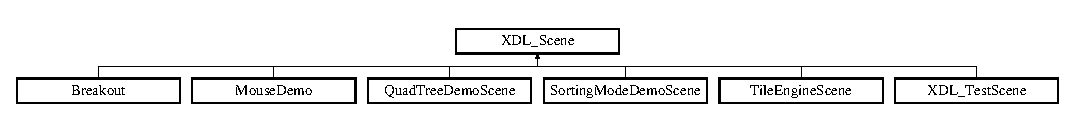
\includegraphics[height=2.000000cm]{class_x_d_l___scene}
\end{center}
\end{figure}
\subsection*{Public Member Functions}
\begin{DoxyCompactItemize}
\item 
\hyperlink{class_x_d_l___scene_abc2c1afb7ab21c4ca3f5f2146786a1ab}{X\-D\-L\-\_\-\-Scene} (void)
\item 
\hyperlink{class_x_d_l___scene_aa2bd0b3f778c179dc2638674efad4509}{$\sim$\-X\-D\-L\-\_\-\-Scene} (void)
\item 
void \hyperlink{class_x_d_l___scene_a14d2c87c4fc3914182de6ec8bf27cf67}{Init} (S\-D\-L\-\_\-\-Renderer $\ast$\hyperlink{class_x_d_l___scene_a923ee55d91647c14f2566f1aa70e3aed}{\-\_\-renderer})
\item 
virtual void \hyperlink{class_x_d_l___scene_a1a3d1b1f6a4f1f4c0834cc1fe29af814}{Draw} ()
\item 
virtual void \hyperlink{class_x_d_l___scene_abd1ce8f1dbc90c4376c99ccd7fd9c024}{Update} ()
\end{DoxyCompactItemize}
\subsection*{Public Attributes}
\begin{DoxyCompactItemize}
\item 
\hyperlink{class_x_d_l___sprite}{X\-D\-L\-\_\-\-Sprite} $\ast$ \hyperlink{class_x_d_l___scene_a92843792b25864d0aec748ca60213e24}{\-\_\-sprite}
\end{DoxyCompactItemize}
\subsection*{Protected Member Functions}
\begin{DoxyCompactItemize}
\item 
virtual bool \hyperlink{class_x_d_l___scene_ab8aa77c9d37e13b4e67f0e1989bcb641}{Add\-Game\-Object\-To\-Scene} (\hyperlink{class_x_d_l___game_object}{X\-D\-L\-\_\-\-Game\-Object} $\ast$\-\_\-gameobject, string \-\_\-id)
\item 
virtual bool \hyperlink{class_x_d_l___scene_aa8aea6a87c3dbd2faa52480907f90d62}{Remove\-Game\-Object\-From\-Scene} (string \-\_\-id)
\item 
virtual \hyperlink{class_x_d_l___game_object}{X\-D\-L\-\_\-\-Game\-Object} $\ast$ \hyperlink{class_x_d_l___scene_a542233e544b861b4e41b7ab86a91e122}{Get\-Game\-Object\-From\-Scene\-Using\-I\-D} (string \-\_\-id)
\end{DoxyCompactItemize}
\subsection*{Protected Attributes}
\begin{DoxyCompactItemize}
\item 
\hyperlink{class_x_d_l___keyboard}{X\-D\-L\-\_\-\-Keyboard} $\ast$ \hyperlink{class_x_d_l___scene_abc53fadb79149e2f41de807070093509}{\-\_\-keyboard}
\item 
\hyperlink{class_x_d_l___sprite_batch}{X\-D\-L\-\_\-\-Sprite\-Batch} $\ast$ \hyperlink{class_x_d_l___scene_acd40bb9e62e836e6a10bfd75b53b74b1}{\-\_\-sprite\-Batch}
\item 
\hyperlink{class_x_d_l___camera}{X\-D\-L\-\_\-\-Camera} $\ast$ \hyperlink{class_x_d_l___scene_a9f432061e3a0b2bcf9166abf9000b753}{\-\_\-camera}
\item 
\hyperlink{class_x_d_l___storage}{X\-D\-L\-\_\-\-Storage} $\ast$ \hyperlink{class_x_d_l___scene_add9dee84c2e4a1adc445fa9c81d79fe4}{\-\_\-persistant\-Storage}
\item 
S\-D\-L\-\_\-\-Renderer $\ast$ \hyperlink{class_x_d_l___scene_a923ee55d91647c14f2566f1aa70e3aed}{\-\_\-renderer}
\item 
map$<$ string, \hyperlink{class_x_d_l___game_object}{X\-D\-L\-\_\-\-Game\-Object} $\ast$ $>$ \hyperlink{class_x_d_l___scene_aad1feb840a1c2925324ccce29fa1d3a4}{\-\_\-game\-Objects\-In\-Scene}
\end{DoxyCompactItemize}


\subsection{Constructor \& Destructor Documentation}
\hypertarget{class_x_d_l___scene_abc2c1afb7ab21c4ca3f5f2146786a1ab}{\index{X\-D\-L\-\_\-\-Scene@{X\-D\-L\-\_\-\-Scene}!X\-D\-L\-\_\-\-Scene@{X\-D\-L\-\_\-\-Scene}}
\index{X\-D\-L\-\_\-\-Scene@{X\-D\-L\-\_\-\-Scene}!XDL_Scene@{X\-D\-L\-\_\-\-Scene}}
\subsubsection[{X\-D\-L\-\_\-\-Scene}]{\setlength{\rightskip}{0pt plus 5cm}X\-D\-L\-\_\-\-Scene\-::\-X\-D\-L\-\_\-\-Scene (
\begin{DoxyParamCaption}
\item[{void}]{}
\end{DoxyParamCaption}
)}}\label{class_x_d_l___scene_abc2c1afb7ab21c4ca3f5f2146786a1ab}
\hypertarget{class_x_d_l___scene_aa2bd0b3f778c179dc2638674efad4509}{\index{X\-D\-L\-\_\-\-Scene@{X\-D\-L\-\_\-\-Scene}!$\sim$\-X\-D\-L\-\_\-\-Scene@{$\sim$\-X\-D\-L\-\_\-\-Scene}}
\index{$\sim$\-X\-D\-L\-\_\-\-Scene@{$\sim$\-X\-D\-L\-\_\-\-Scene}!XDL_Scene@{X\-D\-L\-\_\-\-Scene}}
\subsubsection[{$\sim$\-X\-D\-L\-\_\-\-Scene}]{\setlength{\rightskip}{0pt plus 5cm}X\-D\-L\-\_\-\-Scene\-::$\sim$\-X\-D\-L\-\_\-\-Scene (
\begin{DoxyParamCaption}
\item[{void}]{}
\end{DoxyParamCaption}
)}}\label{class_x_d_l___scene_aa2bd0b3f778c179dc2638674efad4509}


\subsection{Member Function Documentation}
\hypertarget{class_x_d_l___scene_ab8aa77c9d37e13b4e67f0e1989bcb641}{\index{X\-D\-L\-\_\-\-Scene@{X\-D\-L\-\_\-\-Scene}!Add\-Game\-Object\-To\-Scene@{Add\-Game\-Object\-To\-Scene}}
\index{Add\-Game\-Object\-To\-Scene@{Add\-Game\-Object\-To\-Scene}!XDL_Scene@{X\-D\-L\-\_\-\-Scene}}
\subsubsection[{Add\-Game\-Object\-To\-Scene}]{\setlength{\rightskip}{0pt plus 5cm}bool X\-D\-L\-\_\-\-Scene\-::\-Add\-Game\-Object\-To\-Scene (
\begin{DoxyParamCaption}
\item[{{\bf X\-D\-L\-\_\-\-Game\-Object} $\ast$}]{\-\_\-gameobject, }
\item[{string}]{\-\_\-id}
\end{DoxyParamCaption}
)\hspace{0.3cm}{\ttfamily [protected]}, {\ttfamily [virtual]}}}\label{class_x_d_l___scene_ab8aa77c9d37e13b4e67f0e1989bcb641}
\hypertarget{class_x_d_l___scene_a1a3d1b1f6a4f1f4c0834cc1fe29af814}{\index{X\-D\-L\-\_\-\-Scene@{X\-D\-L\-\_\-\-Scene}!Draw@{Draw}}
\index{Draw@{Draw}!XDL_Scene@{X\-D\-L\-\_\-\-Scene}}
\subsubsection[{Draw}]{\setlength{\rightskip}{0pt plus 5cm}void X\-D\-L\-\_\-\-Scene\-::\-Draw (
\begin{DoxyParamCaption}
{}
\end{DoxyParamCaption}
)\hspace{0.3cm}{\ttfamily [virtual]}}}\label{class_x_d_l___scene_a1a3d1b1f6a4f1f4c0834cc1fe29af814}


Reimplemented in \hyperlink{class_level1_ae8e845511c6fcf574f4f94cd0f986751}{Level1}.

\hypertarget{class_x_d_l___scene_a542233e544b861b4e41b7ab86a91e122}{\index{X\-D\-L\-\_\-\-Scene@{X\-D\-L\-\_\-\-Scene}!Get\-Game\-Object\-From\-Scene\-Using\-I\-D@{Get\-Game\-Object\-From\-Scene\-Using\-I\-D}}
\index{Get\-Game\-Object\-From\-Scene\-Using\-I\-D@{Get\-Game\-Object\-From\-Scene\-Using\-I\-D}!XDL_Scene@{X\-D\-L\-\_\-\-Scene}}
\subsubsection[{Get\-Game\-Object\-From\-Scene\-Using\-I\-D}]{\setlength{\rightskip}{0pt plus 5cm}{\bf X\-D\-L\-\_\-\-Game\-Object} $\ast$ X\-D\-L\-\_\-\-Scene\-::\-Get\-Game\-Object\-From\-Scene\-Using\-I\-D (
\begin{DoxyParamCaption}
\item[{string}]{\-\_\-id}
\end{DoxyParamCaption}
)\hspace{0.3cm}{\ttfamily [protected]}, {\ttfamily [virtual]}}}\label{class_x_d_l___scene_a542233e544b861b4e41b7ab86a91e122}
\hypertarget{class_x_d_l___scene_a14d2c87c4fc3914182de6ec8bf27cf67}{\index{X\-D\-L\-\_\-\-Scene@{X\-D\-L\-\_\-\-Scene}!Init@{Init}}
\index{Init@{Init}!XDL_Scene@{X\-D\-L\-\_\-\-Scene}}
\subsubsection[{Init}]{\setlength{\rightskip}{0pt plus 5cm}void X\-D\-L\-\_\-\-Scene\-::\-Init (
\begin{DoxyParamCaption}
\item[{S\-D\-L\-\_\-\-Renderer $\ast$}]{\-\_\-renderer}
\end{DoxyParamCaption}
)}}\label{class_x_d_l___scene_a14d2c87c4fc3914182de6ec8bf27cf67}
\hypertarget{class_x_d_l___scene_aa8aea6a87c3dbd2faa52480907f90d62}{\index{X\-D\-L\-\_\-\-Scene@{X\-D\-L\-\_\-\-Scene}!Remove\-Game\-Object\-From\-Scene@{Remove\-Game\-Object\-From\-Scene}}
\index{Remove\-Game\-Object\-From\-Scene@{Remove\-Game\-Object\-From\-Scene}!XDL_Scene@{X\-D\-L\-\_\-\-Scene}}
\subsubsection[{Remove\-Game\-Object\-From\-Scene}]{\setlength{\rightskip}{0pt plus 5cm}bool X\-D\-L\-\_\-\-Scene\-::\-Remove\-Game\-Object\-From\-Scene (
\begin{DoxyParamCaption}
\item[{string}]{\-\_\-id}
\end{DoxyParamCaption}
)\hspace{0.3cm}{\ttfamily [protected]}, {\ttfamily [virtual]}}}\label{class_x_d_l___scene_aa8aea6a87c3dbd2faa52480907f90d62}
\hypertarget{class_x_d_l___scene_abd1ce8f1dbc90c4376c99ccd7fd9c024}{\index{X\-D\-L\-\_\-\-Scene@{X\-D\-L\-\_\-\-Scene}!Update@{Update}}
\index{Update@{Update}!XDL_Scene@{X\-D\-L\-\_\-\-Scene}}
\subsubsection[{Update}]{\setlength{\rightskip}{0pt plus 5cm}void X\-D\-L\-\_\-\-Scene\-::\-Update (
\begin{DoxyParamCaption}
{}
\end{DoxyParamCaption}
)\hspace{0.3cm}{\ttfamily [virtual]}}}\label{class_x_d_l___scene_abd1ce8f1dbc90c4376c99ccd7fd9c024}


Reimplemented in \hyperlink{class_level1_a26cbf7e692665c1a1250162057583ee4}{Level1}.



\subsection{Member Data Documentation}
\hypertarget{class_x_d_l___scene_a9f432061e3a0b2bcf9166abf9000b753}{\index{X\-D\-L\-\_\-\-Scene@{X\-D\-L\-\_\-\-Scene}!\-\_\-camera@{\-\_\-camera}}
\index{\-\_\-camera@{\-\_\-camera}!XDL_Scene@{X\-D\-L\-\_\-\-Scene}}
\subsubsection[{\-\_\-camera}]{\setlength{\rightskip}{0pt plus 5cm}{\bf X\-D\-L\-\_\-\-Camera}$\ast$ X\-D\-L\-\_\-\-Scene\-::\-\_\-camera\hspace{0.3cm}{\ttfamily [protected]}}}\label{class_x_d_l___scene_a9f432061e3a0b2bcf9166abf9000b753}
\hypertarget{class_x_d_l___scene_aad1feb840a1c2925324ccce29fa1d3a4}{\index{X\-D\-L\-\_\-\-Scene@{X\-D\-L\-\_\-\-Scene}!\-\_\-game\-Objects\-In\-Scene@{\-\_\-game\-Objects\-In\-Scene}}
\index{\-\_\-game\-Objects\-In\-Scene@{\-\_\-game\-Objects\-In\-Scene}!XDL_Scene@{X\-D\-L\-\_\-\-Scene}}
\subsubsection[{\-\_\-game\-Objects\-In\-Scene}]{\setlength{\rightskip}{0pt plus 5cm}map$<$string,{\bf X\-D\-L\-\_\-\-Game\-Object}$\ast$$>$ X\-D\-L\-\_\-\-Scene\-::\-\_\-game\-Objects\-In\-Scene\hspace{0.3cm}{\ttfamily [protected]}}}\label{class_x_d_l___scene_aad1feb840a1c2925324ccce29fa1d3a4}
\hypertarget{class_x_d_l___scene_abc53fadb79149e2f41de807070093509}{\index{X\-D\-L\-\_\-\-Scene@{X\-D\-L\-\_\-\-Scene}!\-\_\-keyboard@{\-\_\-keyboard}}
\index{\-\_\-keyboard@{\-\_\-keyboard}!XDL_Scene@{X\-D\-L\-\_\-\-Scene}}
\subsubsection[{\-\_\-keyboard}]{\setlength{\rightskip}{0pt plus 5cm}{\bf X\-D\-L\-\_\-\-Keyboard}$\ast$ X\-D\-L\-\_\-\-Scene\-::\-\_\-keyboard\hspace{0.3cm}{\ttfamily [protected]}}}\label{class_x_d_l___scene_abc53fadb79149e2f41de807070093509}
\hypertarget{class_x_d_l___scene_add9dee84c2e4a1adc445fa9c81d79fe4}{\index{X\-D\-L\-\_\-\-Scene@{X\-D\-L\-\_\-\-Scene}!\-\_\-persistant\-Storage@{\-\_\-persistant\-Storage}}
\index{\-\_\-persistant\-Storage@{\-\_\-persistant\-Storage}!XDL_Scene@{X\-D\-L\-\_\-\-Scene}}
\subsubsection[{\-\_\-persistant\-Storage}]{\setlength{\rightskip}{0pt plus 5cm}{\bf X\-D\-L\-\_\-\-Storage}$\ast$ X\-D\-L\-\_\-\-Scene\-::\-\_\-persistant\-Storage\hspace{0.3cm}{\ttfamily [protected]}}}\label{class_x_d_l___scene_add9dee84c2e4a1adc445fa9c81d79fe4}
\hypertarget{class_x_d_l___scene_a923ee55d91647c14f2566f1aa70e3aed}{\index{X\-D\-L\-\_\-\-Scene@{X\-D\-L\-\_\-\-Scene}!\-\_\-renderer@{\-\_\-renderer}}
\index{\-\_\-renderer@{\-\_\-renderer}!XDL_Scene@{X\-D\-L\-\_\-\-Scene}}
\subsubsection[{\-\_\-renderer}]{\setlength{\rightskip}{0pt plus 5cm}S\-D\-L\-\_\-\-Renderer$\ast$ X\-D\-L\-\_\-\-Scene\-::\-\_\-renderer\hspace{0.3cm}{\ttfamily [protected]}}}\label{class_x_d_l___scene_a923ee55d91647c14f2566f1aa70e3aed}
\hypertarget{class_x_d_l___scene_a92843792b25864d0aec748ca60213e24}{\index{X\-D\-L\-\_\-\-Scene@{X\-D\-L\-\_\-\-Scene}!\-\_\-sprite@{\-\_\-sprite}}
\index{\-\_\-sprite@{\-\_\-sprite}!XDL_Scene@{X\-D\-L\-\_\-\-Scene}}
\subsubsection[{\-\_\-sprite}]{\setlength{\rightskip}{0pt plus 5cm}{\bf X\-D\-L\-\_\-\-Sprite}$\ast$ X\-D\-L\-\_\-\-Scene\-::\-\_\-sprite}}\label{class_x_d_l___scene_a92843792b25864d0aec748ca60213e24}
\hypertarget{class_x_d_l___scene_acd40bb9e62e836e6a10bfd75b53b74b1}{\index{X\-D\-L\-\_\-\-Scene@{X\-D\-L\-\_\-\-Scene}!\-\_\-sprite\-Batch@{\-\_\-sprite\-Batch}}
\index{\-\_\-sprite\-Batch@{\-\_\-sprite\-Batch}!XDL_Scene@{X\-D\-L\-\_\-\-Scene}}
\subsubsection[{\-\_\-sprite\-Batch}]{\setlength{\rightskip}{0pt plus 5cm}{\bf X\-D\-L\-\_\-\-Sprite\-Batch}$\ast$ X\-D\-L\-\_\-\-Scene\-::\-\_\-sprite\-Batch\hspace{0.3cm}{\ttfamily [protected]}}}\label{class_x_d_l___scene_acd40bb9e62e836e6a10bfd75b53b74b1}


The documentation for this class was generated from the following files\-:\begin{DoxyCompactItemize}
\item 
Joes\-\_\-\-S\-D\-L\-\_\-\-Framework/\hyperlink{_x_d_l___scene_8h}{X\-D\-L\-\_\-\-Scene.\-h}\item 
Joes\-\_\-\-S\-D\-L\-\_\-\-Framework/\hyperlink{_x_d_l___scene_8cpp}{X\-D\-L\-\_\-\-Scene.\-cpp}\end{DoxyCompactItemize}

\hypertarget{class_x_d_l___scene_manager}{\section{X\-D\-L\-\_\-\-Scene\-Manager Class Reference}
\label{class_x_d_l___scene_manager}\index{X\-D\-L\-\_\-\-Scene\-Manager@{X\-D\-L\-\_\-\-Scene\-Manager}}
}


{\ttfamily \#include $<$X\-D\-L\-\_\-\-Scene\-Manager.\-h$>$}

\subsection*{Public Member Functions}
\begin{DoxyCompactItemize}
\item 
\hyperlink{class_x_d_l___scene_manager_acf72aec112908a2c7c694727256cca53}{$\sim$\-X\-D\-L\-\_\-\-Scene\-Manager} (void)
\item 
void \hyperlink{class_x_d_l___scene_manager_af5f8eae12e4346273fb9a2435cfe655b}{Change\-Scene} (\hyperlink{class_x_d_l___scene}{X\-D\-L\-\_\-\-Scene} $\ast$\-\_\-level\-Name, char $\ast$\-\_\-level)
\item 
char $\ast$ \hyperlink{class_x_d_l___scene_manager_ad3c4876932e507a849c54a66b88264de}{Get\-Current\-Scene\-Name} ()
\item 
\hyperlink{class_x_d_l___scene}{X\-D\-L\-\_\-\-Scene} $\ast$ \hyperlink{class_x_d_l___scene_manager_a8adee7ad0ab4cacc98a926848a88c955}{Get\-Current\-Scene} ()
\item 
void \hyperlink{class_x_d_l___scene_manager_a0c7a0611cf19993ce57d71d1f8becc64}{Update} ()
\item 
void \hyperlink{class_x_d_l___scene_manager_a8ec68a45cc1dd459f7154120dfea5b59}{Draw} ()
\end{DoxyCompactItemize}
\subsection*{Static Public Member Functions}
\begin{DoxyCompactItemize}
\item 
static \hyperlink{class_x_d_l___scene_manager}{X\-D\-L\-\_\-\-Scene\-Manager} $\ast$ \hyperlink{class_x_d_l___scene_manager_aee31018d3348547c1c331d05bbb0b039}{Get\-Instance} ()
\end{DoxyCompactItemize}


\subsection{Constructor \& Destructor Documentation}
\hypertarget{class_x_d_l___scene_manager_acf72aec112908a2c7c694727256cca53}{\index{X\-D\-L\-\_\-\-Scene\-Manager@{X\-D\-L\-\_\-\-Scene\-Manager}!$\sim$\-X\-D\-L\-\_\-\-Scene\-Manager@{$\sim$\-X\-D\-L\-\_\-\-Scene\-Manager}}
\index{$\sim$\-X\-D\-L\-\_\-\-Scene\-Manager@{$\sim$\-X\-D\-L\-\_\-\-Scene\-Manager}!XDL_SceneManager@{X\-D\-L\-\_\-\-Scene\-Manager}}
\subsubsection[{$\sim$\-X\-D\-L\-\_\-\-Scene\-Manager}]{\setlength{\rightskip}{0pt plus 5cm}X\-D\-L\-\_\-\-Scene\-Manager\-::$\sim$\-X\-D\-L\-\_\-\-Scene\-Manager (
\begin{DoxyParamCaption}
\item[{void}]{}
\end{DoxyParamCaption}
)}}\label{class_x_d_l___scene_manager_acf72aec112908a2c7c694727256cca53}


\subsection{Member Function Documentation}
\hypertarget{class_x_d_l___scene_manager_af5f8eae12e4346273fb9a2435cfe655b}{\index{X\-D\-L\-\_\-\-Scene\-Manager@{X\-D\-L\-\_\-\-Scene\-Manager}!Change\-Scene@{Change\-Scene}}
\index{Change\-Scene@{Change\-Scene}!XDL_SceneManager@{X\-D\-L\-\_\-\-Scene\-Manager}}
\subsubsection[{Change\-Scene}]{\setlength{\rightskip}{0pt plus 5cm}void X\-D\-L\-\_\-\-Scene\-Manager\-::\-Change\-Scene (
\begin{DoxyParamCaption}
\item[{{\bf X\-D\-L\-\_\-\-Scene} $\ast$}]{\-\_\-level\-Name, }
\item[{char $\ast$}]{\-\_\-level}
\end{DoxyParamCaption}
)}}\label{class_x_d_l___scene_manager_af5f8eae12e4346273fb9a2435cfe655b}
\hypertarget{class_x_d_l___scene_manager_a8ec68a45cc1dd459f7154120dfea5b59}{\index{X\-D\-L\-\_\-\-Scene\-Manager@{X\-D\-L\-\_\-\-Scene\-Manager}!Draw@{Draw}}
\index{Draw@{Draw}!XDL_SceneManager@{X\-D\-L\-\_\-\-Scene\-Manager}}
\subsubsection[{Draw}]{\setlength{\rightskip}{0pt plus 5cm}void X\-D\-L\-\_\-\-Scene\-Manager\-::\-Draw (
\begin{DoxyParamCaption}
{}
\end{DoxyParamCaption}
)}}\label{class_x_d_l___scene_manager_a8ec68a45cc1dd459f7154120dfea5b59}
\hypertarget{class_x_d_l___scene_manager_a8adee7ad0ab4cacc98a926848a88c955}{\index{X\-D\-L\-\_\-\-Scene\-Manager@{X\-D\-L\-\_\-\-Scene\-Manager}!Get\-Current\-Scene@{Get\-Current\-Scene}}
\index{Get\-Current\-Scene@{Get\-Current\-Scene}!XDL_SceneManager@{X\-D\-L\-\_\-\-Scene\-Manager}}
\subsubsection[{Get\-Current\-Scene}]{\setlength{\rightskip}{0pt plus 5cm}{\bf X\-D\-L\-\_\-\-Scene} $\ast$ X\-D\-L\-\_\-\-Scene\-Manager\-::\-Get\-Current\-Scene (
\begin{DoxyParamCaption}
{}
\end{DoxyParamCaption}
)}}\label{class_x_d_l___scene_manager_a8adee7ad0ab4cacc98a926848a88c955}
\hypertarget{class_x_d_l___scene_manager_ad3c4876932e507a849c54a66b88264de}{\index{X\-D\-L\-\_\-\-Scene\-Manager@{X\-D\-L\-\_\-\-Scene\-Manager}!Get\-Current\-Scene\-Name@{Get\-Current\-Scene\-Name}}
\index{Get\-Current\-Scene\-Name@{Get\-Current\-Scene\-Name}!XDL_SceneManager@{X\-D\-L\-\_\-\-Scene\-Manager}}
\subsubsection[{Get\-Current\-Scene\-Name}]{\setlength{\rightskip}{0pt plus 5cm}char $\ast$ X\-D\-L\-\_\-\-Scene\-Manager\-::\-Get\-Current\-Scene\-Name (
\begin{DoxyParamCaption}
{}
\end{DoxyParamCaption}
)}}\label{class_x_d_l___scene_manager_ad3c4876932e507a849c54a66b88264de}
\hypertarget{class_x_d_l___scene_manager_aee31018d3348547c1c331d05bbb0b039}{\index{X\-D\-L\-\_\-\-Scene\-Manager@{X\-D\-L\-\_\-\-Scene\-Manager}!Get\-Instance@{Get\-Instance}}
\index{Get\-Instance@{Get\-Instance}!XDL_SceneManager@{X\-D\-L\-\_\-\-Scene\-Manager}}
\subsubsection[{Get\-Instance}]{\setlength{\rightskip}{0pt plus 5cm}{\bf X\-D\-L\-\_\-\-Scene\-Manager} $\ast$ X\-D\-L\-\_\-\-Scene\-Manager\-::\-Get\-Instance (
\begin{DoxyParamCaption}
{}
\end{DoxyParamCaption}
)\hspace{0.3cm}{\ttfamily [static]}}}\label{class_x_d_l___scene_manager_aee31018d3348547c1c331d05bbb0b039}
\hypertarget{class_x_d_l___scene_manager_a0c7a0611cf19993ce57d71d1f8becc64}{\index{X\-D\-L\-\_\-\-Scene\-Manager@{X\-D\-L\-\_\-\-Scene\-Manager}!Update@{Update}}
\index{Update@{Update}!XDL_SceneManager@{X\-D\-L\-\_\-\-Scene\-Manager}}
\subsubsection[{Update}]{\setlength{\rightskip}{0pt plus 5cm}void X\-D\-L\-\_\-\-Scene\-Manager\-::\-Update (
\begin{DoxyParamCaption}
{}
\end{DoxyParamCaption}
)}}\label{class_x_d_l___scene_manager_a0c7a0611cf19993ce57d71d1f8becc64}


The documentation for this class was generated from the following files\-:\begin{DoxyCompactItemize}
\item 
Joes\-\_\-\-S\-D\-L\-\_\-\-Framework/\hyperlink{_x_d_l___scene_manager_8h}{X\-D\-L\-\_\-\-Scene\-Manager.\-h}\item 
Joes\-\_\-\-S\-D\-L\-\_\-\-Framework/\hyperlink{_x_d_l___scene_manager_8cpp}{X\-D\-L\-\_\-\-Scene\-Manager.\-cpp}\end{DoxyCompactItemize}

\hypertarget{class_x_d_l___sprite}{\section{X\-D\-L\-\_\-\-Sprite Class Reference}
\label{class_x_d_l___sprite}\index{X\-D\-L\-\_\-\-Sprite@{X\-D\-L\-\_\-\-Sprite}}
}


\hyperlink{class_x_d_l___sprite}{X\-D\-L\-\_\-\-Sprite}.  




{\ttfamily \#include $<$X\-D\-L\-\_\-\-Sprite.\-h$>$}

Inheritance diagram for X\-D\-L\-\_\-\-Sprite\-:\begin{figure}[H]
\begin{center}
\leavevmode
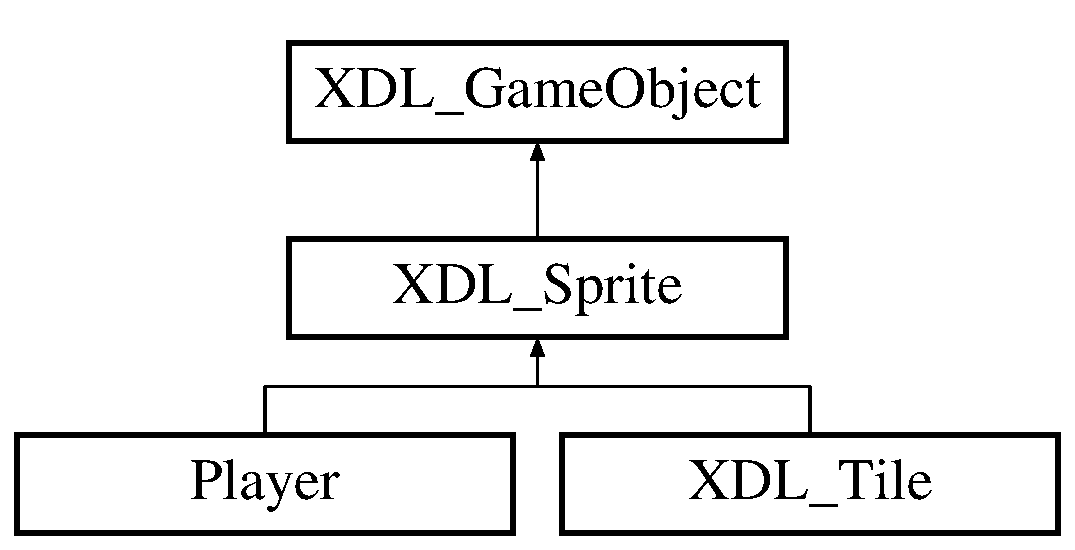
\includegraphics[height=3.000000cm]{class_x_d_l___sprite}
\end{center}
\end{figure}
\subsection*{Public Member Functions}
\begin{DoxyCompactItemize}
\item 
\hyperlink{class_x_d_l___sprite_a17aa0483052cf03519f4885966ee8e1b}{X\-D\-L\-\_\-\-Sprite} (char $\ast$\-\_\-asset, float \-\_\-x, float \-\_\-y, int \-\_\-height, int \-\_\-width, int \hyperlink{class_x_d_l___game_object_a62a08106992c783507c669f71a6dd6a6}{\-\_\-z}, S\-D\-L\-\_\-\-Renderer $\ast$\-\_\-renderer, string \-\_\-unique\-Name)
\item 
\hyperlink{class_x_d_l___sprite_a1be30c1e18f81665dbf8833faaa29925}{X\-D\-L\-\_\-\-Sprite} (char $\ast$\-\_\-asset, float \-\_\-x, float \-\_\-y, int \-\_\-height, int \-\_\-width, int \hyperlink{class_x_d_l___game_object_a62a08106992c783507c669f71a6dd6a6}{\-\_\-z}, S\-D\-L\-\_\-\-Renderer $\ast$\-\_\-renderer, S\-D\-L\-\_\-\-Rect \-\_\-source\-Rect, string \-\_\-unique\-Name)
\item 
\hyperlink{class_x_d_l___sprite_accb0cd8b6f2b18c3f5927082fc057b8d}{X\-D\-L\-\_\-\-Sprite} (char $\ast$\-\_\-asset, float \-\_\-x, float \-\_\-y, int \-\_\-height, int \-\_\-width, int \hyperlink{class_x_d_l___game_object_a62a08106992c783507c669f71a6dd6a6}{\-\_\-z}, S\-D\-L\-\_\-\-Renderer $\ast$\-\_\-renderer, S\-D\-L\-\_\-\-Rect \-\_\-source\-Rect, int \-\_\-num\-Frames, string \-\_\-unique\-Name)
\item 
\hypertarget{class_x_d_l___sprite_a1ecd6d713ce320cd1d49dceea854e0d2}{virtual void {\bfseries Update} ()}\label{class_x_d_l___sprite_a1ecd6d713ce320cd1d49dceea854e0d2}

\item 
virtual void \hyperlink{class_x_d_l___sprite_a5b1c9b886c59f06cfbb2c428b3f58e86}{Draw} ()
\item 
\hypertarget{class_x_d_l___sprite_af594d7e5987b56ea146e640b9ced33b2}{virtual void {\bfseries Animate} ()}\label{class_x_d_l___sprite_af594d7e5987b56ea146e640b9ced33b2}

\end{DoxyCompactItemize}
\subsection*{Protected Member Functions}
\begin{DoxyCompactItemize}
\item 
\hypertarget{class_x_d_l___sprite_a30ef3609e3bb1a36dea1d6bf3d5628f4}{void {\bfseries Init} (char $\ast$\-\_\-asset, float \-\_\-x, float \-\_\-y, int \-\_\-height, int \-\_\-width, S\-D\-L\-\_\-\-Renderer $\ast$\-\_\-renderer)}\label{class_x_d_l___sprite_a30ef3609e3bb1a36dea1d6bf3d5628f4}

\end{DoxyCompactItemize}
\subsection*{Protected Attributes}
\begin{DoxyCompactItemize}
\item 
\hypertarget{class_x_d_l___sprite_aedcf07ef73df095eb6cd9843870cd002}{S\-D\-L\-\_\-\-Renderer $\ast$ {\bfseries \-\_\-renderer}}\label{class_x_d_l___sprite_aedcf07ef73df095eb6cd9843870cd002}

\item 
\hypertarget{class_x_d_l___sprite_a64b44e17128d166f81a5ad0a3f1f0130}{int {\bfseries \-\_\-num\-Frames}}\label{class_x_d_l___sprite_a64b44e17128d166f81a5ad0a3f1f0130}

\item 
\hypertarget{class_x_d_l___sprite_a400af77ad887dec8bdb210e04299259a}{int {\bfseries \-\_\-current\-Frame}}\label{class_x_d_l___sprite_a400af77ad887dec8bdb210e04299259a}

\item 
\hypertarget{class_x_d_l___sprite_a98c75cc4f4abc07331ad8de391a19675}{S\-D\-L\-\_\-\-Rect {\bfseries \-\_\-source\-Rect}}\label{class_x_d_l___sprite_a98c75cc4f4abc07331ad8de391a19675}

\item 
\hypertarget{class_x_d_l___sprite_ad83f66f89a449230516e37534a228af7}{S\-D\-L\-\_\-\-Rect {\bfseries \-\_\-draw\-Rect}}\label{class_x_d_l___sprite_ad83f66f89a449230516e37534a228af7}

\item 
\hypertarget{class_x_d_l___sprite_a8e385099b36a25f00322acd2b353751e}{S\-D\-L\-\_\-\-Texture $\ast$ {\bfseries \-\_\-texture}}\label{class_x_d_l___sprite_a8e385099b36a25f00322acd2b353751e}

\item 
\hypertarget{class_x_d_l___sprite_a8e50211a0f424c3a77753a206232f9ef}{const char $\ast$ {\bfseries \-\_\-asset\-Name}}\label{class_x_d_l___sprite_a8e50211a0f424c3a77753a206232f9ef}

\item 
\hypertarget{class_x_d_l___sprite_a39231e3b79b80ebb38cc9c9d5e1b4323}{\hyperlink{class_x_d_l___content_manager}{X\-D\-L\-\_\-\-Content\-Manager} $\ast$ {\bfseries \-\_\-content}}\label{class_x_d_l___sprite_a39231e3b79b80ebb38cc9c9d5e1b4323}

\end{DoxyCompactItemize}
\subsection*{Additional Inherited Members}


\subsection{Detailed Description}
\hyperlink{class_x_d_l___sprite}{X\-D\-L\-\_\-\-Sprite}. 

Extension of Game\-Object

Provides extra functionality, such as a sprite visual element, and loading/drawing from tilesheets 

\subsection{Constructor \& Destructor Documentation}
\hypertarget{class_x_d_l___sprite_a17aa0483052cf03519f4885966ee8e1b}{\index{X\-D\-L\-\_\-\-Sprite@{X\-D\-L\-\_\-\-Sprite}!X\-D\-L\-\_\-\-Sprite@{X\-D\-L\-\_\-\-Sprite}}
\index{X\-D\-L\-\_\-\-Sprite@{X\-D\-L\-\_\-\-Sprite}!XDL_Sprite@{X\-D\-L\-\_\-\-Sprite}}
\subsubsection[{X\-D\-L\-\_\-\-Sprite}]{\setlength{\rightskip}{0pt plus 5cm}X\-D\-L\-\_\-\-Sprite\-::\-X\-D\-L\-\_\-\-Sprite (
\begin{DoxyParamCaption}
\item[{char $\ast$}]{\-\_\-asset, }
\item[{float}]{\-\_\-x, }
\item[{float}]{\-\_\-y, }
\item[{int}]{\-\_\-width, }
\item[{int}]{\-\_\-height, }
\item[{int}]{\-\_\-z, }
\item[{S\-D\-L\-\_\-\-Renderer $\ast$}]{\-\_\-renderer, }
\item[{string}]{\-\_\-unique\-Name}
\end{DoxyParamCaption}
)}}\label{class_x_d_l___sprite_a17aa0483052cf03519f4885966ee8e1b}
constructor for file, where we are going to draw the entire image \hypertarget{class_x_d_l___sprite_a1be30c1e18f81665dbf8833faaa29925}{\index{X\-D\-L\-\_\-\-Sprite@{X\-D\-L\-\_\-\-Sprite}!X\-D\-L\-\_\-\-Sprite@{X\-D\-L\-\_\-\-Sprite}}
\index{X\-D\-L\-\_\-\-Sprite@{X\-D\-L\-\_\-\-Sprite}!XDL_Sprite@{X\-D\-L\-\_\-\-Sprite}}
\subsubsection[{X\-D\-L\-\_\-\-Sprite}]{\setlength{\rightskip}{0pt plus 5cm}X\-D\-L\-\_\-\-Sprite\-::\-X\-D\-L\-\_\-\-Sprite (
\begin{DoxyParamCaption}
\item[{char $\ast$}]{\-\_\-asset, }
\item[{float}]{\-\_\-x, }
\item[{float}]{\-\_\-y, }
\item[{int}]{\-\_\-width, }
\item[{int}]{\-\_\-height, }
\item[{int}]{\-\_\-z, }
\item[{S\-D\-L\-\_\-\-Renderer $\ast$}]{\-\_\-renderer, }
\item[{S\-D\-L\-\_\-\-Rect}]{\-\_\-source\-Rect, }
\item[{string}]{\-\_\-unique\-Name}
\end{DoxyParamCaption}
)}}\label{class_x_d_l___sprite_a1be30c1e18f81665dbf8833faaa29925}
constructor for use with tilesheets. \hypertarget{class_x_d_l___sprite_accb0cd8b6f2b18c3f5927082fc057b8d}{\index{X\-D\-L\-\_\-\-Sprite@{X\-D\-L\-\_\-\-Sprite}!X\-D\-L\-\_\-\-Sprite@{X\-D\-L\-\_\-\-Sprite}}
\index{X\-D\-L\-\_\-\-Sprite@{X\-D\-L\-\_\-\-Sprite}!XDL_Sprite@{X\-D\-L\-\_\-\-Sprite}}
\subsubsection[{X\-D\-L\-\_\-\-Sprite}]{\setlength{\rightskip}{0pt plus 5cm}X\-D\-L\-\_\-\-Sprite\-::\-X\-D\-L\-\_\-\-Sprite (
\begin{DoxyParamCaption}
\item[{char $\ast$}]{\-\_\-asset, }
\item[{float}]{\-\_\-x, }
\item[{float}]{\-\_\-y, }
\item[{int}]{\-\_\-height, }
\item[{int}]{\-\_\-width, }
\item[{int}]{\-\_\-z, }
\item[{S\-D\-L\-\_\-\-Renderer $\ast$}]{\-\_\-renderer, }
\item[{S\-D\-L\-\_\-\-Rect}]{\-\_\-source\-Rect, }
\item[{int}]{\-\_\-num\-Frames, }
\item[{string}]{\-\_\-unique\-Name}
\end{DoxyParamCaption}
)}}\label{class_x_d_l___sprite_accb0cd8b6f2b18c3f5927082fc057b8d}
constructor for use with animation...which is no implemented yet 

\subsection{Member Function Documentation}
\hypertarget{class_x_d_l___sprite_a5b1c9b886c59f06cfbb2c428b3f58e86}{\index{X\-D\-L\-\_\-\-Sprite@{X\-D\-L\-\_\-\-Sprite}!Draw@{Draw}}
\index{Draw@{Draw}!XDL_Sprite@{X\-D\-L\-\_\-\-Sprite}}
\subsubsection[{Draw}]{\setlength{\rightskip}{0pt plus 5cm}void X\-D\-L\-\_\-\-Sprite\-::\-Draw (
\begin{DoxyParamCaption}
{}
\end{DoxyParamCaption}
)\hspace{0.3cm}{\ttfamily [virtual]}}}\label{class_x_d_l___sprite_a5b1c9b886c59f06cfbb2c428b3f58e86}
virtual function so every object that is added to the scene will get auto-\/updated 

Implements \hyperlink{class_x_d_l___game_object_a46ab89c9622631cf13114a493b1b0a2d}{X\-D\-L\-\_\-\-Game\-Object}.



Reimplemented in \hyperlink{class_path_finding_sprite_a1fdc88d9b985f6f7b7ce8de4eaa31a5a}{Path\-Finding\-Sprite}, and \hyperlink{class_demo_mover_sprite_a4dae3800a23e9ed5f68cd83b05be8ab8}{Demo\-Mover\-Sprite}.



The documentation for this class was generated from the following files\-:\begin{DoxyCompactItemize}
\item 
Joes\-\_\-\-S\-D\-L\-\_\-\-Framework/X\-D\-L\-\_\-\-Sprite.\-h\item 
Joes\-\_\-\-S\-D\-L\-\_\-\-Framework/X\-D\-L\-\_\-\-Sprite.\-cpp\end{DoxyCompactItemize}

\hypertarget{class_x_d_l___sprite_batch}{\section{X\-D\-L\-\_\-\-Sprite\-Batch Class Reference}
\label{class_x_d_l___sprite_batch}\index{X\-D\-L\-\_\-\-Sprite\-Batch@{X\-D\-L\-\_\-\-Sprite\-Batch}}
}
\subsection*{Public Types}
\begin{DoxyCompactItemize}
\item 
enum \hyperlink{class_x_d_l___sprite_batch_a0dba0557842cdf21917adc2ef44125e6}{D\-R\-A\-W\-M\-O\-D\-E\-S} \{ {\bfseries F\-R\-O\-N\-T\-T\-O\-B\-A\-C\-K}, 
\hyperlink{class_x_d_l___sprite_batch_a0dba0557842cdf21917adc2ef44125e6af0aff02dad6d665eb8a61c108e5ca1d1}{B\-A\-C\-K\-T\-O\-F\-R\-O\-N\-T}, 
\hyperlink{class_x_d_l___sprite_batch_a0dba0557842cdf21917adc2ef44125e6a4dea32cd64020138077648d29c34f58a}{U\-N\-S\-O\-R\-T\-E\-D}
 \}
\end{DoxyCompactItemize}
\subsection*{Public Member Functions}
\begin{DoxyCompactItemize}
\item 
\hypertarget{class_x_d_l___sprite_batch_a0ee6240197106c7ad2061226da69ba47}{void {\bfseries Init} (S\-D\-L\-\_\-\-Renderer $\ast$\-\_\-renderer, int \-\_\-world\-Size\-X, int \-\_\-world\-Size\-Y)}\label{class_x_d_l___sprite_batch_a0ee6240197106c7ad2061226da69ba47}

\item 
\hypertarget{class_x_d_l___sprite_batch_af6db9acdec8c4b1f31275b24d99d50d4}{void {\bfseries Begin} ()}\label{class_x_d_l___sprite_batch_af6db9acdec8c4b1f31275b24d99d50d4}

\item 
\hypertarget{class_x_d_l___sprite_batch_a63a34e3458a687841c8a9c3d1de876b6}{void {\bfseries Draw} (\hyperlink{class_x_d_l___game_object}{X\-D\-L\-\_\-\-Game\-Object} $\ast$\-\_\-me)}\label{class_x_d_l___sprite_batch_a63a34e3458a687841c8a9c3d1de876b6}

\item 
\hypertarget{class_x_d_l___sprite_batch_a60d1f227cf1ef2270f58711b6d37a20f}{void {\bfseries End} ()}\label{class_x_d_l___sprite_batch_a60d1f227cf1ef2270f58711b6d37a20f}

\item 
\hypertarget{class_x_d_l___sprite_batch_a696b70cf462c9bad88f255f3f8a79506}{void {\bfseries Set\-Draw\-Mode} (\hyperlink{class_x_d_l___sprite_batch_a0dba0557842cdf21917adc2ef44125e6}{D\-R\-A\-W\-M\-O\-D\-E\-S} \-\_\-drawmode)}\label{class_x_d_l___sprite_batch_a696b70cf462c9bad88f255f3f8a79506}

\item 
\hypertarget{class_x_d_l___sprite_batch_a48fa9280c8a1dc5c93a3732adacca526}{int {\bfseries Get\-Draw\-Mode} ()}\label{class_x_d_l___sprite_batch_a48fa9280c8a1dc5c93a3732adacca526}

\item 
\hypertarget{class_x_d_l___sprite_batch_aff9895e54f671c94c83613731c11fc2e}{void {\bfseries Set\-Camera} (\hyperlink{class_x_d_l___camera}{X\-D\-L\-\_\-\-Camera} $\ast$X\-D\-L\-\_\-\-C\-A\-M\-E\-R\-A)}\label{class_x_d_l___sprite_batch_aff9895e54f671c94c83613731c11fc2e}

\item 
\hypertarget{class_x_d_l___sprite_batch_a32ddb6e2d599029bc2e6de79c8437210}{\hyperlink{class_x_d_l___camera}{X\-D\-L\-\_\-\-Camera} $\ast$ {\bfseries Get\-Camera} ()}\label{class_x_d_l___sprite_batch_a32ddb6e2d599029bc2e6de79c8437210}

\end{DoxyCompactItemize}
\subsection*{Static Public Member Functions}
\begin{DoxyCompactItemize}
\item 
\hypertarget{class_x_d_l___sprite_batch_a1a5318ca5a0a82603f96453793afa6d0}{static \hyperlink{class_x_d_l___sprite_batch}{X\-D\-L\-\_\-\-Sprite\-Batch} $\ast$ {\bfseries Get\-Instance} ()}\label{class_x_d_l___sprite_batch_a1a5318ca5a0a82603f96453793afa6d0}

\end{DoxyCompactItemize}
\subsection*{Public Attributes}
\begin{DoxyCompactItemize}
\item 
\hypertarget{class_x_d_l___sprite_batch_afcee76b702fbc3794783ab86c73cf8d0}{S\-D\-L\-\_\-\-Rect {\bfseries \-\_\-draw\-Rect}}\label{class_x_d_l___sprite_batch_afcee76b702fbc3794783ab86c73cf8d0}

\item 
\hypertarget{class_x_d_l___sprite_batch_a8ce0db8774bbedf72939f071ac02f100}{S\-D\-L\-\_\-\-Rect $\ast$ {\bfseries \-\_\-draw\-Texture\-Bounds}}\label{class_x_d_l___sprite_batch_a8ce0db8774bbedf72939f071ac02f100}

\end{DoxyCompactItemize}
\subsection*{Static Public Attributes}
\begin{DoxyCompactItemize}
\item 
\hypertarget{class_x_d_l___sprite_batch_a37476782380898a316c9bb7a09aeee0d}{static S\-D\-L\-\_\-\-Texture $\ast$ {\bfseries \-\_\-draw\-Texture}}\label{class_x_d_l___sprite_batch_a37476782380898a316c9bb7a09aeee0d}

\end{DoxyCompactItemize}


\subsection{Member Enumeration Documentation}
\hypertarget{class_x_d_l___sprite_batch_a0dba0557842cdf21917adc2ef44125e6}{\index{X\-D\-L\-\_\-\-Sprite\-Batch@{X\-D\-L\-\_\-\-Sprite\-Batch}!D\-R\-A\-W\-M\-O\-D\-E\-S@{D\-R\-A\-W\-M\-O\-D\-E\-S}}
\index{D\-R\-A\-W\-M\-O\-D\-E\-S@{D\-R\-A\-W\-M\-O\-D\-E\-S}!XDL_SpriteBatch@{X\-D\-L\-\_\-\-Sprite\-Batch}}
\subsubsection[{D\-R\-A\-W\-M\-O\-D\-E\-S}]{\setlength{\rightskip}{0pt plus 5cm}enum {\bf X\-D\-L\-\_\-\-Sprite\-Batch\-::\-D\-R\-A\-W\-M\-O\-D\-E\-S}}}\label{class_x_d_l___sprite_batch_a0dba0557842cdf21917adc2ef44125e6}
\begin{Desc}
\item[Enumerator]\par
\begin{description}
\index{B\-A\-C\-K\-T\-O\-F\-R\-O\-N\-T@{B\-A\-C\-K\-T\-O\-F\-R\-O\-N\-T}!X\-D\-L\-\_\-\-Sprite\-Batch@{X\-D\-L\-\_\-\-Sprite\-Batch}}\index{X\-D\-L\-\_\-\-Sprite\-Batch@{X\-D\-L\-\_\-\-Sprite\-Batch}!B\-A\-C\-K\-T\-O\-F\-R\-O\-N\-T@{B\-A\-C\-K\-T\-O\-F\-R\-O\-N\-T}}\item[{\em 
\hypertarget{class_x_d_l___sprite_batch_a0dba0557842cdf21917adc2ef44125e6af0aff02dad6d665eb8a61c108e5ca1d1}{B\-A\-C\-K\-T\-O\-F\-R\-O\-N\-T}\label{class_x_d_l___sprite_batch_a0dba0557842cdf21917adc2ef44125e6af0aff02dad6d665eb8a61c108e5ca1d1}
}]Larger Z means drawn at the back. \index{U\-N\-S\-O\-R\-T\-E\-D@{U\-N\-S\-O\-R\-T\-E\-D}!X\-D\-L\-\_\-\-Sprite\-Batch@{X\-D\-L\-\_\-\-Sprite\-Batch}}\index{X\-D\-L\-\_\-\-Sprite\-Batch@{X\-D\-L\-\_\-\-Sprite\-Batch}!U\-N\-S\-O\-R\-T\-E\-D@{U\-N\-S\-O\-R\-T\-E\-D}}\item[{\em 
\hypertarget{class_x_d_l___sprite_batch_a0dba0557842cdf21917adc2ef44125e6a4dea32cd64020138077648d29c34f58a}{U\-N\-S\-O\-R\-T\-E\-D}\label{class_x_d_l___sprite_batch_a0dba0557842cdf21917adc2ef44125e6a4dea32cd64020138077648d29c34f58a}
}]Smaller Z's drawn in the back, bigger Z drawn in front

no sorting, drawn in same order as they are added \end{description}
\end{Desc}


The documentation for this class was generated from the following files\-:\begin{DoxyCompactItemize}
\item 
Joes\-\_\-\-S\-D\-L\-\_\-\-Framework/X\-D\-L\-\_\-\-Sprite\-Batch.\-h\item 
Joes\-\_\-\-S\-D\-L\-\_\-\-Framework/X\-D\-L\-\_\-\-Sprite\-Batch.\-cpp\end{DoxyCompactItemize}

\hypertarget{class_x_d_l___storage}{\section{X\-D\-L\-\_\-\-Storage Class Reference}
\label{class_x_d_l___storage}\index{X\-D\-L\-\_\-\-Storage@{X\-D\-L\-\_\-\-Storage}}
}


{\ttfamily \#include $<$X\-D\-L\-\_\-\-Storage.\-h$>$}

\subsection*{Public Member Functions}
\begin{DoxyCompactItemize}
\item 
\hyperlink{class_x_d_l___storage_af13cd722d2f622b672dc364e95b0cb86}{$\sim$\-X\-D\-L\-\_\-\-Storage} (void)
\item 
void \hyperlink{class_x_d_l___storage_af0cc2938516ff6a2410dd6920888bd7f}{Save\-Int} (int \-\_\-value, char $\ast$\-\_\-id)
\item 
void \hyperlink{class_x_d_l___storage_ad1893c5d3dfbbb0037a1eed6ed1abcbc}{Save\-Char\-Pointer} (char $\ast$\-\_\-value, char $\ast$\-\_\-id)
\item 
void \hyperlink{class_x_d_l___storage_afcd7763d1f4d31b9f05d46d22cfd30b5}{Save\-Float} (float \-\_\-value, char $\ast$\-\_\-id)
\item 
int \hyperlink{class_x_d_l___storage_a21526a669339830f7d40214ca011aa2e}{Load\-Int} (char $\ast$\-\_\-id)
\item 
char $\ast$ \hyperlink{class_x_d_l___storage_a82a1d30c23688ff94441e5976e8d48ff}{Load\-Char\-Pointer} (char $\ast$\-\_\-id)
\item 
float \hyperlink{class_x_d_l___storage_af9d042c604cd818d96220819ea38bfbe}{Load\-Float} (char $\ast$\-\_\-id)
\end{DoxyCompactItemize}
\subsection*{Static Public Member Functions}
\begin{DoxyCompactItemize}
\item 
static \hyperlink{class_x_d_l___storage}{X\-D\-L\-\_\-\-Storage} $\ast$ \hyperlink{class_x_d_l___storage_aacfe0fd0ae64589f641f4139996a0778}{Get\-Instance} ()
\end{DoxyCompactItemize}


\subsection{Constructor \& Destructor Documentation}
\hypertarget{class_x_d_l___storage_af13cd722d2f622b672dc364e95b0cb86}{\index{X\-D\-L\-\_\-\-Storage@{X\-D\-L\-\_\-\-Storage}!$\sim$\-X\-D\-L\-\_\-\-Storage@{$\sim$\-X\-D\-L\-\_\-\-Storage}}
\index{$\sim$\-X\-D\-L\-\_\-\-Storage@{$\sim$\-X\-D\-L\-\_\-\-Storage}!XDL_Storage@{X\-D\-L\-\_\-\-Storage}}
\subsubsection[{$\sim$\-X\-D\-L\-\_\-\-Storage}]{\setlength{\rightskip}{0pt plus 5cm}X\-D\-L\-\_\-\-Storage\-::$\sim$\-X\-D\-L\-\_\-\-Storage (
\begin{DoxyParamCaption}
\item[{void}]{}
\end{DoxyParamCaption}
)}}\label{class_x_d_l___storage_af13cd722d2f622b672dc364e95b0cb86}


\subsection{Member Function Documentation}
\hypertarget{class_x_d_l___storage_aacfe0fd0ae64589f641f4139996a0778}{\index{X\-D\-L\-\_\-\-Storage@{X\-D\-L\-\_\-\-Storage}!Get\-Instance@{Get\-Instance}}
\index{Get\-Instance@{Get\-Instance}!XDL_Storage@{X\-D\-L\-\_\-\-Storage}}
\subsubsection[{Get\-Instance}]{\setlength{\rightskip}{0pt plus 5cm}{\bf X\-D\-L\-\_\-\-Storage} $\ast$ X\-D\-L\-\_\-\-Storage\-::\-Get\-Instance (
\begin{DoxyParamCaption}
{}
\end{DoxyParamCaption}
)\hspace{0.3cm}{\ttfamily [static]}}}\label{class_x_d_l___storage_aacfe0fd0ae64589f641f4139996a0778}
\hypertarget{class_x_d_l___storage_a82a1d30c23688ff94441e5976e8d48ff}{\index{X\-D\-L\-\_\-\-Storage@{X\-D\-L\-\_\-\-Storage}!Load\-Char\-Pointer@{Load\-Char\-Pointer}}
\index{Load\-Char\-Pointer@{Load\-Char\-Pointer}!XDL_Storage@{X\-D\-L\-\_\-\-Storage}}
\subsubsection[{Load\-Char\-Pointer}]{\setlength{\rightskip}{0pt plus 5cm}char $\ast$ X\-D\-L\-\_\-\-Storage\-::\-Load\-Char\-Pointer (
\begin{DoxyParamCaption}
\item[{char $\ast$}]{\-\_\-id}
\end{DoxyParamCaption}
)}}\label{class_x_d_l___storage_a82a1d30c23688ff94441e5976e8d48ff}
\hypertarget{class_x_d_l___storage_af9d042c604cd818d96220819ea38bfbe}{\index{X\-D\-L\-\_\-\-Storage@{X\-D\-L\-\_\-\-Storage}!Load\-Float@{Load\-Float}}
\index{Load\-Float@{Load\-Float}!XDL_Storage@{X\-D\-L\-\_\-\-Storage}}
\subsubsection[{Load\-Float}]{\setlength{\rightskip}{0pt plus 5cm}float X\-D\-L\-\_\-\-Storage\-::\-Load\-Float (
\begin{DoxyParamCaption}
\item[{char $\ast$}]{\-\_\-id}
\end{DoxyParamCaption}
)}}\label{class_x_d_l___storage_af9d042c604cd818d96220819ea38bfbe}
\hypertarget{class_x_d_l___storage_a21526a669339830f7d40214ca011aa2e}{\index{X\-D\-L\-\_\-\-Storage@{X\-D\-L\-\_\-\-Storage}!Load\-Int@{Load\-Int}}
\index{Load\-Int@{Load\-Int}!XDL_Storage@{X\-D\-L\-\_\-\-Storage}}
\subsubsection[{Load\-Int}]{\setlength{\rightskip}{0pt plus 5cm}int X\-D\-L\-\_\-\-Storage\-::\-Load\-Int (
\begin{DoxyParamCaption}
\item[{char $\ast$}]{\-\_\-id}
\end{DoxyParamCaption}
)}}\label{class_x_d_l___storage_a21526a669339830f7d40214ca011aa2e}
\hypertarget{class_x_d_l___storage_ad1893c5d3dfbbb0037a1eed6ed1abcbc}{\index{X\-D\-L\-\_\-\-Storage@{X\-D\-L\-\_\-\-Storage}!Save\-Char\-Pointer@{Save\-Char\-Pointer}}
\index{Save\-Char\-Pointer@{Save\-Char\-Pointer}!XDL_Storage@{X\-D\-L\-\_\-\-Storage}}
\subsubsection[{Save\-Char\-Pointer}]{\setlength{\rightskip}{0pt plus 5cm}void X\-D\-L\-\_\-\-Storage\-::\-Save\-Char\-Pointer (
\begin{DoxyParamCaption}
\item[{char $\ast$}]{\-\_\-value, }
\item[{char $\ast$}]{\-\_\-id}
\end{DoxyParamCaption}
)}}\label{class_x_d_l___storage_ad1893c5d3dfbbb0037a1eed6ed1abcbc}
\hypertarget{class_x_d_l___storage_afcd7763d1f4d31b9f05d46d22cfd30b5}{\index{X\-D\-L\-\_\-\-Storage@{X\-D\-L\-\_\-\-Storage}!Save\-Float@{Save\-Float}}
\index{Save\-Float@{Save\-Float}!XDL_Storage@{X\-D\-L\-\_\-\-Storage}}
\subsubsection[{Save\-Float}]{\setlength{\rightskip}{0pt plus 5cm}void X\-D\-L\-\_\-\-Storage\-::\-Save\-Float (
\begin{DoxyParamCaption}
\item[{float}]{\-\_\-value, }
\item[{char $\ast$}]{\-\_\-id}
\end{DoxyParamCaption}
)}}\label{class_x_d_l___storage_afcd7763d1f4d31b9f05d46d22cfd30b5}
\hypertarget{class_x_d_l___storage_af0cc2938516ff6a2410dd6920888bd7f}{\index{X\-D\-L\-\_\-\-Storage@{X\-D\-L\-\_\-\-Storage}!Save\-Int@{Save\-Int}}
\index{Save\-Int@{Save\-Int}!XDL_Storage@{X\-D\-L\-\_\-\-Storage}}
\subsubsection[{Save\-Int}]{\setlength{\rightskip}{0pt plus 5cm}void X\-D\-L\-\_\-\-Storage\-::\-Save\-Int (
\begin{DoxyParamCaption}
\item[{int}]{\-\_\-value, }
\item[{char $\ast$}]{\-\_\-id}
\end{DoxyParamCaption}
)}}\label{class_x_d_l___storage_af0cc2938516ff6a2410dd6920888bd7f}


The documentation for this class was generated from the following files\-:\begin{DoxyCompactItemize}
\item 
Joes\-\_\-\-S\-D\-L\-\_\-\-Framework/\hyperlink{_x_d_l___storage_8h}{X\-D\-L\-\_\-\-Storage.\-h}\item 
Joes\-\_\-\-S\-D\-L\-\_\-\-Framework/\hyperlink{_x_d_l___storage_8cpp}{X\-D\-L\-\_\-\-Storage.\-cpp}\end{DoxyCompactItemize}

\hypertarget{class_x_d_l___tile}{\section{X\-D\-L\-\_\-\-Tile Class Reference}
\label{class_x_d_l___tile}\index{X\-D\-L\-\_\-\-Tile@{X\-D\-L\-\_\-\-Tile}}
}


\hyperlink{class_x_d_l___tile}{X\-D\-L\-\_\-\-Tile}.  




{\ttfamily \#include $<$X\-D\-L\-\_\-\-Tile.\-h$>$}

Inheritance diagram for X\-D\-L\-\_\-\-Tile\-:\begin{figure}[H]
\begin{center}
\leavevmode
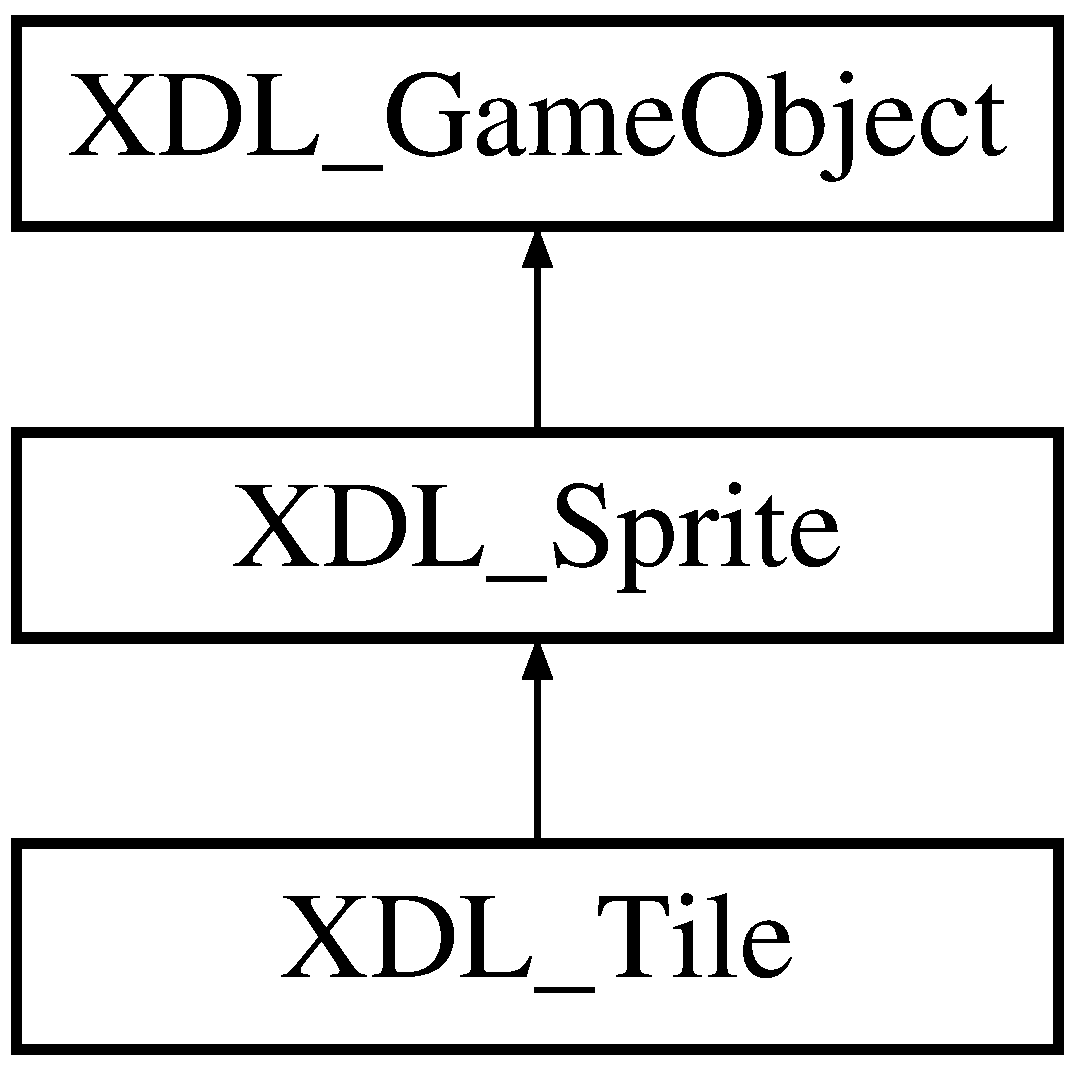
\includegraphics[height=3.000000cm]{class_x_d_l___tile}
\end{center}
\end{figure}
\subsection*{Public Member Functions}
\begin{DoxyCompactItemize}
\item 
\hyperlink{class_x_d_l___tile_ad4e32024eec22bada0f17b0e9ec70008}{X\-D\-L\-\_\-\-Tile} (char $\ast$\-\_\-asset, int \-\_\-x, int \-\_\-y, int \-\_\-height, int \-\_\-width, S\-D\-L\-\_\-\-Renderer $\ast$\hyperlink{class_x_d_l___sprite_aedcf07ef73df095eb6cd9843870cd002}{\-\_\-renderer}, S\-D\-L\-\_\-\-Rect \hyperlink{class_x_d_l___sprite_a98c75cc4f4abc07331ad8de391a19675}{\-\_\-source\-Rect}, int \hyperlink{class_x_d_l___tile_aeb90ee0ab5ad7a0d061fd0e56bbbcee6}{\-\_\-gid})
\item 
virtual \hyperlink{class_x_d_l___tile_a15faa07f0ed8a8192ad7e83cb15878ef}{$\sim$\-X\-D\-L\-\_\-\-Tile} (void)
\item 
void \hyperlink{class_x_d_l___tile_ac520d114e26b99eea8762516a9e4fc0b}{Set\-Parent} (\hyperlink{class_x_d_l___tile}{X\-D\-L\-\_\-\-Tile} $\ast$\-\_\-parent)
\item 
\hyperlink{class_x_d_l___tile}{X\-D\-L\-\_\-\-Tile} $\ast$ \hyperlink{class_x_d_l___tile_a7000f395eee7999beffead93d979a83e}{Get\-Parent} ()
\end{DoxyCompactItemize}
\subsection*{Public Attributes}
\begin{DoxyCompactItemize}
\item 
int \hyperlink{class_x_d_l___tile_aeb90ee0ab5ad7a0d061fd0e56bbbcee6}{\-\_\-gid}
\end{DoxyCompactItemize}
\subsection*{Additional Inherited Members}


\subsection{Detailed Description}
\hyperlink{class_x_d_l___tile}{X\-D\-L\-\_\-\-Tile}. 

Used in \hyperlink{class_x_d_l___tile_engine}{X\-D\-L\-\_\-\-Tile\-Engine}, inherits from sprite, and adds extra variables and functions to allow pathfinding etc. 

\subsection{Constructor \& Destructor Documentation}
\hypertarget{class_x_d_l___tile_ad4e32024eec22bada0f17b0e9ec70008}{\index{X\-D\-L\-\_\-\-Tile@{X\-D\-L\-\_\-\-Tile}!X\-D\-L\-\_\-\-Tile@{X\-D\-L\-\_\-\-Tile}}
\index{X\-D\-L\-\_\-\-Tile@{X\-D\-L\-\_\-\-Tile}!XDL_Tile@{X\-D\-L\-\_\-\-Tile}}
\subsubsection[{X\-D\-L\-\_\-\-Tile}]{\setlength{\rightskip}{0pt plus 5cm}X\-D\-L\-\_\-\-Tile\-::\-X\-D\-L\-\_\-\-Tile (
\begin{DoxyParamCaption}
\item[{char $\ast$}]{\-\_\-asset, }
\item[{int}]{\-\_\-x, }
\item[{int}]{\-\_\-y, }
\item[{int}]{\-\_\-height, }
\item[{int}]{\-\_\-width, }
\item[{S\-D\-L\-\_\-\-Renderer $\ast$}]{\-\_\-renderer, }
\item[{S\-D\-L\-\_\-\-Rect}]{\-\_\-source\-Rect, }
\item[{int}]{\-\_\-gid}
\end{DoxyParamCaption}
)}}\label{class_x_d_l___tile_ad4e32024eec22bada0f17b0e9ec70008}
\hypertarget{class_x_d_l___tile_a15faa07f0ed8a8192ad7e83cb15878ef}{\index{X\-D\-L\-\_\-\-Tile@{X\-D\-L\-\_\-\-Tile}!$\sim$\-X\-D\-L\-\_\-\-Tile@{$\sim$\-X\-D\-L\-\_\-\-Tile}}
\index{$\sim$\-X\-D\-L\-\_\-\-Tile@{$\sim$\-X\-D\-L\-\_\-\-Tile}!XDL_Tile@{X\-D\-L\-\_\-\-Tile}}
\subsubsection[{$\sim$\-X\-D\-L\-\_\-\-Tile}]{\setlength{\rightskip}{0pt plus 5cm}X\-D\-L\-\_\-\-Tile\-::$\sim$\-X\-D\-L\-\_\-\-Tile (
\begin{DoxyParamCaption}
\item[{void}]{}
\end{DoxyParamCaption}
)\hspace{0.3cm}{\ttfamily [virtual]}}}\label{class_x_d_l___tile_a15faa07f0ed8a8192ad7e83cb15878ef}


\subsection{Member Function Documentation}
\hypertarget{class_x_d_l___tile_a7000f395eee7999beffead93d979a83e}{\index{X\-D\-L\-\_\-\-Tile@{X\-D\-L\-\_\-\-Tile}!Get\-Parent@{Get\-Parent}}
\index{Get\-Parent@{Get\-Parent}!XDL_Tile@{X\-D\-L\-\_\-\-Tile}}
\subsubsection[{Get\-Parent}]{\setlength{\rightskip}{0pt plus 5cm}{\bf X\-D\-L\-\_\-\-Tile} $\ast$ X\-D\-L\-\_\-\-Tile\-::\-Get\-Parent (
\begin{DoxyParamCaption}
{}
\end{DoxyParamCaption}
)}}\label{class_x_d_l___tile_a7000f395eee7999beffead93d979a83e}
\hypertarget{class_x_d_l___tile_ac520d114e26b99eea8762516a9e4fc0b}{\index{X\-D\-L\-\_\-\-Tile@{X\-D\-L\-\_\-\-Tile}!Set\-Parent@{Set\-Parent}}
\index{Set\-Parent@{Set\-Parent}!XDL_Tile@{X\-D\-L\-\_\-\-Tile}}
\subsubsection[{Set\-Parent}]{\setlength{\rightskip}{0pt plus 5cm}void X\-D\-L\-\_\-\-Tile\-::\-Set\-Parent (
\begin{DoxyParamCaption}
\item[{{\bf X\-D\-L\-\_\-\-Tile} $\ast$}]{\-\_\-parent}
\end{DoxyParamCaption}
)}}\label{class_x_d_l___tile_ac520d114e26b99eea8762516a9e4fc0b}


\subsection{Member Data Documentation}
\hypertarget{class_x_d_l___tile_aeb90ee0ab5ad7a0d061fd0e56bbbcee6}{\index{X\-D\-L\-\_\-\-Tile@{X\-D\-L\-\_\-\-Tile}!\-\_\-gid@{\-\_\-gid}}
\index{\-\_\-gid@{\-\_\-gid}!XDL_Tile@{X\-D\-L\-\_\-\-Tile}}
\subsubsection[{\-\_\-gid}]{\setlength{\rightskip}{0pt plus 5cm}int X\-D\-L\-\_\-\-Tile\-::\-\_\-gid}}\label{class_x_d_l___tile_aeb90ee0ab5ad7a0d061fd0e56bbbcee6}


The documentation for this class was generated from the following files\-:\begin{DoxyCompactItemize}
\item 
Joes\-\_\-\-S\-D\-L\-\_\-\-Framework/\hyperlink{_x_d_l___tile_8h}{X\-D\-L\-\_\-\-Tile.\-h}\item 
Joes\-\_\-\-S\-D\-L\-\_\-\-Framework/\hyperlink{_x_d_l___tile_8cpp}{X\-D\-L\-\_\-\-Tile.\-cpp}\end{DoxyCompactItemize}

\hypertarget{class_x_d_l___tile_engine}{\section{X\-D\-L\-\_\-\-Tile\-Engine Class Reference}
\label{class_x_d_l___tile_engine}\index{X\-D\-L\-\_\-\-Tile\-Engine@{X\-D\-L\-\_\-\-Tile\-Engine}}
}


{\ttfamily \#include $<$X\-D\-L\-\_\-\-Tile\-Engine.\-h$>$}

\subsection*{Public Member Functions}
\begin{DoxyCompactItemize}
\item 
\hyperlink{class_x_d_l___tile_engine_a98bee762bf2317a9835fe08d43c72d3e}{X\-D\-L\-\_\-\-Tile\-Engine} (S\-D\-L\-\_\-\-Renderer $\ast$\-\_\-renderer, int \-\_\-tiles\-Width, int \-\_\-tiles\-Height)
\item 
\hyperlink{class_x_d_l___tile_engine_a821e376c855b2a35a26c42d7c3536798}{$\sim$\-X\-D\-L\-\_\-\-Tile\-Engine} (void)
\item 
void \hyperlink{class_x_d_l___tile_engine_a09b4b351ebcb85a637c6324eca20f7ae}{Update} ()
\item 
void \hyperlink{class_x_d_l___tile_engine_ac64a769f7337304d90d9597fd9cd9a41}{Draw} (\hyperlink{class_x_d_l___sprite_batch}{X\-D\-L\-\_\-\-Sprite\-Batch} $\ast$\-\_\-sprite\-Batch)
\item 
bool \hyperlink{class_x_d_l___tile_engine_a768bab50a988a2bb6f329709fb57f5ce}{Load\-From\-X\-M\-L} (char $\ast$\-\_\-path\-To\-T\-M\-X)
\item 
bool \hyperlink{class_x_d_l___tile_engine_a8f6d9ab1bd0bb21d403cde2e5980cb9d}{Load\-From\-T\-M\-X\-And\-T\-S\-X} (char $\ast$\-\_\-path\-To\-T\-M\-X)
\item 
int \hyperlink{class_x_d_l___tile_engine_acc054aba7cc81238b2101f562fdeaeed}{Get\-Tile\-Width} ()
\item 
int \hyperlink{class_x_d_l___tile_engine_a5c7c48bcfc59c2e0c5c03dad43c52d7a}{Get\-Tile\-Height} ()
\item 
\hyperlink{class_x_d_l___layer}{X\-D\-L\-\_\-\-Layer} $\ast$ \hyperlink{class_x_d_l___tile_engine_aab7ccf749e184493f526bbdab9a22f96}{Get\-Layer} (int layer\-Num)
\end{DoxyCompactItemize}


\subsection{Constructor \& Destructor Documentation}
\hypertarget{class_x_d_l___tile_engine_a98bee762bf2317a9835fe08d43c72d3e}{\index{X\-D\-L\-\_\-\-Tile\-Engine@{X\-D\-L\-\_\-\-Tile\-Engine}!X\-D\-L\-\_\-\-Tile\-Engine@{X\-D\-L\-\_\-\-Tile\-Engine}}
\index{X\-D\-L\-\_\-\-Tile\-Engine@{X\-D\-L\-\_\-\-Tile\-Engine}!XDL_TileEngine@{X\-D\-L\-\_\-\-Tile\-Engine}}
\subsubsection[{X\-D\-L\-\_\-\-Tile\-Engine}]{\setlength{\rightskip}{0pt plus 5cm}X\-D\-L\-\_\-\-Tile\-Engine\-::\-X\-D\-L\-\_\-\-Tile\-Engine (
\begin{DoxyParamCaption}
\item[{S\-D\-L\-\_\-\-Renderer $\ast$}]{\-\_\-renderer, }
\item[{int}]{\-\_\-tiles\-Width, }
\item[{int}]{\-\_\-tiles\-Height}
\end{DoxyParamCaption}
)}}\label{class_x_d_l___tile_engine_a98bee762bf2317a9835fe08d43c72d3e}
\hypertarget{class_x_d_l___tile_engine_a821e376c855b2a35a26c42d7c3536798}{\index{X\-D\-L\-\_\-\-Tile\-Engine@{X\-D\-L\-\_\-\-Tile\-Engine}!$\sim$\-X\-D\-L\-\_\-\-Tile\-Engine@{$\sim$\-X\-D\-L\-\_\-\-Tile\-Engine}}
\index{$\sim$\-X\-D\-L\-\_\-\-Tile\-Engine@{$\sim$\-X\-D\-L\-\_\-\-Tile\-Engine}!XDL_TileEngine@{X\-D\-L\-\_\-\-Tile\-Engine}}
\subsubsection[{$\sim$\-X\-D\-L\-\_\-\-Tile\-Engine}]{\setlength{\rightskip}{0pt plus 5cm}X\-D\-L\-\_\-\-Tile\-Engine\-::$\sim$\-X\-D\-L\-\_\-\-Tile\-Engine (
\begin{DoxyParamCaption}
\item[{void}]{}
\end{DoxyParamCaption}
)}}\label{class_x_d_l___tile_engine_a821e376c855b2a35a26c42d7c3536798}


\subsection{Member Function Documentation}
\hypertarget{class_x_d_l___tile_engine_ac64a769f7337304d90d9597fd9cd9a41}{\index{X\-D\-L\-\_\-\-Tile\-Engine@{X\-D\-L\-\_\-\-Tile\-Engine}!Draw@{Draw}}
\index{Draw@{Draw}!XDL_TileEngine@{X\-D\-L\-\_\-\-Tile\-Engine}}
\subsubsection[{Draw}]{\setlength{\rightskip}{0pt plus 5cm}void X\-D\-L\-\_\-\-Tile\-Engine\-::\-Draw (
\begin{DoxyParamCaption}
\item[{{\bf X\-D\-L\-\_\-\-Sprite\-Batch} $\ast$}]{\-\_\-sprite\-Batch}
\end{DoxyParamCaption}
)}}\label{class_x_d_l___tile_engine_ac64a769f7337304d90d9597fd9cd9a41}
\hypertarget{class_x_d_l___tile_engine_aab7ccf749e184493f526bbdab9a22f96}{\index{X\-D\-L\-\_\-\-Tile\-Engine@{X\-D\-L\-\_\-\-Tile\-Engine}!Get\-Layer@{Get\-Layer}}
\index{Get\-Layer@{Get\-Layer}!XDL_TileEngine@{X\-D\-L\-\_\-\-Tile\-Engine}}
\subsubsection[{Get\-Layer}]{\setlength{\rightskip}{0pt plus 5cm}{\bf X\-D\-L\-\_\-\-Layer} $\ast$ X\-D\-L\-\_\-\-Tile\-Engine\-::\-Get\-Layer (
\begin{DoxyParamCaption}
\item[{int}]{layer\-Num}
\end{DoxyParamCaption}
)}}\label{class_x_d_l___tile_engine_aab7ccf749e184493f526bbdab9a22f96}
\hypertarget{class_x_d_l___tile_engine_a5c7c48bcfc59c2e0c5c03dad43c52d7a}{\index{X\-D\-L\-\_\-\-Tile\-Engine@{X\-D\-L\-\_\-\-Tile\-Engine}!Get\-Tile\-Height@{Get\-Tile\-Height}}
\index{Get\-Tile\-Height@{Get\-Tile\-Height}!XDL_TileEngine@{X\-D\-L\-\_\-\-Tile\-Engine}}
\subsubsection[{Get\-Tile\-Height}]{\setlength{\rightskip}{0pt plus 5cm}int X\-D\-L\-\_\-\-Tile\-Engine\-::\-Get\-Tile\-Height (
\begin{DoxyParamCaption}
{}
\end{DoxyParamCaption}
)}}\label{class_x_d_l___tile_engine_a5c7c48bcfc59c2e0c5c03dad43c52d7a}
\hypertarget{class_x_d_l___tile_engine_acc054aba7cc81238b2101f562fdeaeed}{\index{X\-D\-L\-\_\-\-Tile\-Engine@{X\-D\-L\-\_\-\-Tile\-Engine}!Get\-Tile\-Width@{Get\-Tile\-Width}}
\index{Get\-Tile\-Width@{Get\-Tile\-Width}!XDL_TileEngine@{X\-D\-L\-\_\-\-Tile\-Engine}}
\subsubsection[{Get\-Tile\-Width}]{\setlength{\rightskip}{0pt plus 5cm}int X\-D\-L\-\_\-\-Tile\-Engine\-::\-Get\-Tile\-Width (
\begin{DoxyParamCaption}
{}
\end{DoxyParamCaption}
)}}\label{class_x_d_l___tile_engine_acc054aba7cc81238b2101f562fdeaeed}
\hypertarget{class_x_d_l___tile_engine_a8f6d9ab1bd0bb21d403cde2e5980cb9d}{\index{X\-D\-L\-\_\-\-Tile\-Engine@{X\-D\-L\-\_\-\-Tile\-Engine}!Load\-From\-T\-M\-X\-And\-T\-S\-X@{Load\-From\-T\-M\-X\-And\-T\-S\-X}}
\index{Load\-From\-T\-M\-X\-And\-T\-S\-X@{Load\-From\-T\-M\-X\-And\-T\-S\-X}!XDL_TileEngine@{X\-D\-L\-\_\-\-Tile\-Engine}}
\subsubsection[{Load\-From\-T\-M\-X\-And\-T\-S\-X}]{\setlength{\rightskip}{0pt plus 5cm}bool X\-D\-L\-\_\-\-Tile\-Engine\-::\-Load\-From\-T\-M\-X\-And\-T\-S\-X (
\begin{DoxyParamCaption}
\item[{char $\ast$}]{\-\_\-path\-To\-T\-M\-X}
\end{DoxyParamCaption}
)}}\label{class_x_d_l___tile_engine_a8f6d9ab1bd0bb21d403cde2e5980cb9d}
\hypertarget{class_x_d_l___tile_engine_a768bab50a988a2bb6f329709fb57f5ce}{\index{X\-D\-L\-\_\-\-Tile\-Engine@{X\-D\-L\-\_\-\-Tile\-Engine}!Load\-From\-X\-M\-L@{Load\-From\-X\-M\-L}}
\index{Load\-From\-X\-M\-L@{Load\-From\-X\-M\-L}!XDL_TileEngine@{X\-D\-L\-\_\-\-Tile\-Engine}}
\subsubsection[{Load\-From\-X\-M\-L}]{\setlength{\rightskip}{0pt plus 5cm}bool X\-D\-L\-\_\-\-Tile\-Engine\-::\-Load\-From\-X\-M\-L (
\begin{DoxyParamCaption}
\item[{char $\ast$}]{\-\_\-path\-To\-T\-M\-X}
\end{DoxyParamCaption}
)}}\label{class_x_d_l___tile_engine_a768bab50a988a2bb6f329709fb57f5ce}
\hypertarget{class_x_d_l___tile_engine_a09b4b351ebcb85a637c6324eca20f7ae}{\index{X\-D\-L\-\_\-\-Tile\-Engine@{X\-D\-L\-\_\-\-Tile\-Engine}!Update@{Update}}
\index{Update@{Update}!XDL_TileEngine@{X\-D\-L\-\_\-\-Tile\-Engine}}
\subsubsection[{Update}]{\setlength{\rightskip}{0pt plus 5cm}void X\-D\-L\-\_\-\-Tile\-Engine\-::\-Update (
\begin{DoxyParamCaption}
{}
\end{DoxyParamCaption}
)}}\label{class_x_d_l___tile_engine_a09b4b351ebcb85a637c6324eca20f7ae}


The documentation for this class was generated from the following files\-:\begin{DoxyCompactItemize}
\item 
Joes\-\_\-\-S\-D\-L\-\_\-\-Framework/\hyperlink{_x_d_l___tile_engine_8h}{X\-D\-L\-\_\-\-Tile\-Engine.\-h}\item 
Joes\-\_\-\-S\-D\-L\-\_\-\-Framework/\hyperlink{_x_d_l___tile_engine_8cpp}{X\-D\-L\-\_\-\-Tile\-Engine.\-cpp}\end{DoxyCompactItemize}

\hypertarget{classtinyxml2_1_1_x_m_l_attribute}{\section{tinyxml2\-:\-:X\-M\-L\-Attribute Class Reference}
\label{classtinyxml2_1_1_x_m_l_attribute}\index{tinyxml2\-::\-X\-M\-L\-Attribute@{tinyxml2\-::\-X\-M\-L\-Attribute}}
}


{\ttfamily \#include $<$tinyxml2.\-h$>$}

\subsection*{Public Member Functions}
\begin{DoxyCompactItemize}
\item 
\hypertarget{classtinyxml2_1_1_x_m_l_attribute_a631990ac0d176e38fc291b17b295a62d}{const char $\ast$ \hyperlink{classtinyxml2_1_1_x_m_l_attribute_a631990ac0d176e38fc291b17b295a62d}{Name} () const }\label{classtinyxml2_1_1_x_m_l_attribute_a631990ac0d176e38fc291b17b295a62d}

\begin{DoxyCompactList}\small\item\em The name of the attribute. \end{DoxyCompactList}\item 
\hypertarget{classtinyxml2_1_1_x_m_l_attribute_adf884db24f469f8a99a14ae786d4ddd7}{const char $\ast$ \hyperlink{classtinyxml2_1_1_x_m_l_attribute_adf884db24f469f8a99a14ae786d4ddd7}{Value} () const }\label{classtinyxml2_1_1_x_m_l_attribute_adf884db24f469f8a99a14ae786d4ddd7}

\begin{DoxyCompactList}\small\item\em The value of the attribute. \end{DoxyCompactList}\item 
\hypertarget{classtinyxml2_1_1_x_m_l_attribute_a7fd852d6185af90361ec1bc9a7681ad6}{const \hyperlink{classtinyxml2_1_1_x_m_l_attribute}{X\-M\-L\-Attribute} $\ast$ \hyperlink{classtinyxml2_1_1_x_m_l_attribute_a7fd852d6185af90361ec1bc9a7681ad6}{Next} () const }\label{classtinyxml2_1_1_x_m_l_attribute_a7fd852d6185af90361ec1bc9a7681ad6}

\begin{DoxyCompactList}\small\item\em The next attribute in the list. \end{DoxyCompactList}\item 
int \hyperlink{classtinyxml2_1_1_x_m_l_attribute_a949d02a5888092cc68c1e29185301863}{Int\-Value} () const 
\item 
\hypertarget{classtinyxml2_1_1_x_m_l_attribute_a4c7a179907836a136d1ce5acbe53389d}{unsigned \hyperlink{classtinyxml2_1_1_x_m_l_attribute_a4c7a179907836a136d1ce5acbe53389d}{Unsigned\-Value} () const }\label{classtinyxml2_1_1_x_m_l_attribute_a4c7a179907836a136d1ce5acbe53389d}

\begin{DoxyCompactList}\small\item\em Query as an unsigned integer. See \hyperlink{classtinyxml2_1_1_x_m_l_attribute_a949d02a5888092cc68c1e29185301863}{Int\-Value()} \end{DoxyCompactList}\item 
\hypertarget{classtinyxml2_1_1_x_m_l_attribute_afb444b7a12527f836aa161b54b2f7ce7}{bool \hyperlink{classtinyxml2_1_1_x_m_l_attribute_afb444b7a12527f836aa161b54b2f7ce7}{Bool\-Value} () const }\label{classtinyxml2_1_1_x_m_l_attribute_afb444b7a12527f836aa161b54b2f7ce7}

\begin{DoxyCompactList}\small\item\em Query as a boolean. See \hyperlink{classtinyxml2_1_1_x_m_l_attribute_a949d02a5888092cc68c1e29185301863}{Int\-Value()} \end{DoxyCompactList}\item 
\hypertarget{classtinyxml2_1_1_x_m_l_attribute_a336153e5aa1b7ccd6502fc249bfb3fd7}{double \hyperlink{classtinyxml2_1_1_x_m_l_attribute_a336153e5aa1b7ccd6502fc249bfb3fd7}{Double\-Value} () const }\label{classtinyxml2_1_1_x_m_l_attribute_a336153e5aa1b7ccd6502fc249bfb3fd7}

\begin{DoxyCompactList}\small\item\em Query as a double. See \hyperlink{classtinyxml2_1_1_x_m_l_attribute_a949d02a5888092cc68c1e29185301863}{Int\-Value()} \end{DoxyCompactList}\item 
\hypertarget{classtinyxml2_1_1_x_m_l_attribute_ae3d51ff98eacc1dc46efcfdaee5c84ad}{float \hyperlink{classtinyxml2_1_1_x_m_l_attribute_ae3d51ff98eacc1dc46efcfdaee5c84ad}{Float\-Value} () const }\label{classtinyxml2_1_1_x_m_l_attribute_ae3d51ff98eacc1dc46efcfdaee5c84ad}

\begin{DoxyCompactList}\small\item\em Query as a float. See \hyperlink{classtinyxml2_1_1_x_m_l_attribute_a949d02a5888092cc68c1e29185301863}{Int\-Value()} \end{DoxyCompactList}\item 
X\-M\-L\-Error \hyperlink{classtinyxml2_1_1_x_m_l_attribute_ad510a83c4ff2755844bb250b125d28ff}{Query\-Int\-Value} (int $\ast$value) const 
\item 
\hypertarget{classtinyxml2_1_1_x_m_l_attribute_ac93f5981adfd62ac4ea76bfa668ee2b4}{X\-M\-L\-Error \hyperlink{classtinyxml2_1_1_x_m_l_attribute_ac93f5981adfd62ac4ea76bfa668ee2b4}{Query\-Unsigned\-Value} (unsigned int $\ast$value) const }\label{classtinyxml2_1_1_x_m_l_attribute_ac93f5981adfd62ac4ea76bfa668ee2b4}

\begin{DoxyCompactList}\small\item\em See Query\-Int\-Value. \end{DoxyCompactList}\item 
\hypertarget{classtinyxml2_1_1_x_m_l_attribute_a9e9b94369f182df72aaac9acd04afead}{X\-M\-L\-Error \hyperlink{classtinyxml2_1_1_x_m_l_attribute_a9e9b94369f182df72aaac9acd04afead}{Query\-Bool\-Value} (bool $\ast$value) const }\label{classtinyxml2_1_1_x_m_l_attribute_a9e9b94369f182df72aaac9acd04afead}

\begin{DoxyCompactList}\small\item\em See Query\-Int\-Value. \end{DoxyCompactList}\item 
\hypertarget{classtinyxml2_1_1_x_m_l_attribute_a0872c05edea2a7cde4bd96c1e9cb2fc4}{X\-M\-L\-Error \hyperlink{classtinyxml2_1_1_x_m_l_attribute_a0872c05edea2a7cde4bd96c1e9cb2fc4}{Query\-Double\-Value} (double $\ast$value) const }\label{classtinyxml2_1_1_x_m_l_attribute_a0872c05edea2a7cde4bd96c1e9cb2fc4}

\begin{DoxyCompactList}\small\item\em See Query\-Int\-Value. \end{DoxyCompactList}\item 
\hypertarget{classtinyxml2_1_1_x_m_l_attribute_afb254627c296d1d70b755397d32fece8}{X\-M\-L\-Error \hyperlink{classtinyxml2_1_1_x_m_l_attribute_afb254627c296d1d70b755397d32fece8}{Query\-Float\-Value} (float $\ast$value) const }\label{classtinyxml2_1_1_x_m_l_attribute_afb254627c296d1d70b755397d32fece8}

\begin{DoxyCompactList}\small\item\em See Query\-Int\-Value. \end{DoxyCompactList}\item 
\hypertarget{classtinyxml2_1_1_x_m_l_attribute_a406d2c4a13c7af99a65edb59dd9f7581}{void \hyperlink{classtinyxml2_1_1_x_m_l_attribute_a406d2c4a13c7af99a65edb59dd9f7581}{Set\-Attribute} (const char $\ast$value)}\label{classtinyxml2_1_1_x_m_l_attribute_a406d2c4a13c7af99a65edb59dd9f7581}

\begin{DoxyCompactList}\small\item\em Set the attribute to a string value. \end{DoxyCompactList}\item 
\hypertarget{classtinyxml2_1_1_x_m_l_attribute_ad86d7d7058d76761c3a80662566a57e5}{void \hyperlink{classtinyxml2_1_1_x_m_l_attribute_ad86d7d7058d76761c3a80662566a57e5}{Set\-Attribute} (int value)}\label{classtinyxml2_1_1_x_m_l_attribute_ad86d7d7058d76761c3a80662566a57e5}

\begin{DoxyCompactList}\small\item\em Set the attribute to value. \end{DoxyCompactList}\item 
\hypertarget{classtinyxml2_1_1_x_m_l_attribute_ae70468c0f6df2748ba3529c716999fae}{void \hyperlink{classtinyxml2_1_1_x_m_l_attribute_ae70468c0f6df2748ba3529c716999fae}{Set\-Attribute} (unsigned value)}\label{classtinyxml2_1_1_x_m_l_attribute_ae70468c0f6df2748ba3529c716999fae}

\begin{DoxyCompactList}\small\item\em Set the attribute to value. \end{DoxyCompactList}\item 
\hypertarget{classtinyxml2_1_1_x_m_l_attribute_ab3516def4fe058fe328f2b89fc2d77da}{void \hyperlink{classtinyxml2_1_1_x_m_l_attribute_ab3516def4fe058fe328f2b89fc2d77da}{Set\-Attribute} (bool value)}\label{classtinyxml2_1_1_x_m_l_attribute_ab3516def4fe058fe328f2b89fc2d77da}

\begin{DoxyCompactList}\small\item\em Set the attribute to value. \end{DoxyCompactList}\item 
\hypertarget{classtinyxml2_1_1_x_m_l_attribute_a9a65ab3147abe8ccbbd373ce8791e818}{void \hyperlink{classtinyxml2_1_1_x_m_l_attribute_a9a65ab3147abe8ccbbd373ce8791e818}{Set\-Attribute} (double value)}\label{classtinyxml2_1_1_x_m_l_attribute_a9a65ab3147abe8ccbbd373ce8791e818}

\begin{DoxyCompactList}\small\item\em Set the attribute to value. \end{DoxyCompactList}\item 
\hypertarget{classtinyxml2_1_1_x_m_l_attribute_ae95e843313aaf5d56c32530b6456df02}{void \hyperlink{classtinyxml2_1_1_x_m_l_attribute_ae95e843313aaf5d56c32530b6456df02}{Set\-Attribute} (float value)}\label{classtinyxml2_1_1_x_m_l_attribute_ae95e843313aaf5d56c32530b6456df02}

\begin{DoxyCompactList}\small\item\em Set the attribute to value. \end{DoxyCompactList}\end{DoxyCompactItemize}
\subsection*{Friends}
\begin{DoxyCompactItemize}
\item 
\hypertarget{classtinyxml2_1_1_x_m_l_attribute_ac2fba9b6e452829dd892f7392c24e0eb}{class {\bfseries X\-M\-L\-Element}}\label{classtinyxml2_1_1_x_m_l_attribute_ac2fba9b6e452829dd892f7392c24e0eb}

\end{DoxyCompactItemize}


\subsection{Detailed Description}
An attribute is a name-\/value pair. Elements have an arbitrary number of attributes, each with a unique name.

\begin{DoxyNote}{Note}
The attributes are not X\-M\-L\-Nodes. You may only query the \hyperlink{classtinyxml2_1_1_x_m_l_attribute_a7fd852d6185af90361ec1bc9a7681ad6}{Next()} attribute in a list. 
\end{DoxyNote}


\subsection{Member Function Documentation}
\hypertarget{classtinyxml2_1_1_x_m_l_attribute_a949d02a5888092cc68c1e29185301863}{\index{tinyxml2\-::\-X\-M\-L\-Attribute@{tinyxml2\-::\-X\-M\-L\-Attribute}!Int\-Value@{Int\-Value}}
\index{Int\-Value@{Int\-Value}!tinyxml2::XMLAttribute@{tinyxml2\-::\-X\-M\-L\-Attribute}}
\subsubsection[{Int\-Value}]{\setlength{\rightskip}{0pt plus 5cm}int tinyxml2\-::\-X\-M\-L\-Attribute\-::\-Int\-Value (
\begin{DoxyParamCaption}
{}
\end{DoxyParamCaption}
) const\hspace{0.3cm}{\ttfamily [inline]}}}\label{classtinyxml2_1_1_x_m_l_attribute_a949d02a5888092cc68c1e29185301863}
Int\-Value interprets the attribute as an integer, and returns the value. If the value isn't an integer, 0 will be returned. There is no error checking; use \hyperlink{classtinyxml2_1_1_x_m_l_attribute_ad510a83c4ff2755844bb250b125d28ff}{Query\-Int\-Value()} if you need error checking. \hypertarget{classtinyxml2_1_1_x_m_l_attribute_ad510a83c4ff2755844bb250b125d28ff}{\index{tinyxml2\-::\-X\-M\-L\-Attribute@{tinyxml2\-::\-X\-M\-L\-Attribute}!Query\-Int\-Value@{Query\-Int\-Value}}
\index{Query\-Int\-Value@{Query\-Int\-Value}!tinyxml2::XMLAttribute@{tinyxml2\-::\-X\-M\-L\-Attribute}}
\subsubsection[{Query\-Int\-Value}]{\setlength{\rightskip}{0pt plus 5cm}X\-M\-L\-Error tinyxml2\-::\-X\-M\-L\-Attribute\-::\-Query\-Int\-Value (
\begin{DoxyParamCaption}
\item[{int $\ast$}]{value}
\end{DoxyParamCaption}
) const}}\label{classtinyxml2_1_1_x_m_l_attribute_ad510a83c4ff2755844bb250b125d28ff}
Query\-Int\-Value interprets the attribute as an integer, and returns the value in the provided parameter. The function will return X\-M\-L\-\_\-\-N\-O\-\_\-\-E\-R\-R\-O\-R on success, and X\-M\-L\-\_\-\-W\-R\-O\-N\-G\-\_\-\-A\-T\-T\-R\-I\-B\-U\-T\-E\-\_\-\-T\-Y\-P\-E if the conversion is not successful. 

The documentation for this class was generated from the following files\-:\begin{DoxyCompactItemize}
\item 
Joes\-\_\-\-S\-D\-L\-\_\-\-Framework/tinyxml2.\-h\item 
Joes\-\_\-\-S\-D\-L\-\_\-\-Framework/tinyxml2.\-cpp\end{DoxyCompactItemize}

\hypertarget{classtinyxml2_1_1_x_m_l_comment}{\section{tinyxml2\-:\-:X\-M\-L\-Comment Class Reference}
\label{classtinyxml2_1_1_x_m_l_comment}\index{tinyxml2\-::\-X\-M\-L\-Comment@{tinyxml2\-::\-X\-M\-L\-Comment}}
}


{\ttfamily \#include $<$tinyxml2.\-h$>$}

Inheritance diagram for tinyxml2\-:\-:X\-M\-L\-Comment\-:\begin{figure}[H]
\begin{center}
\leavevmode
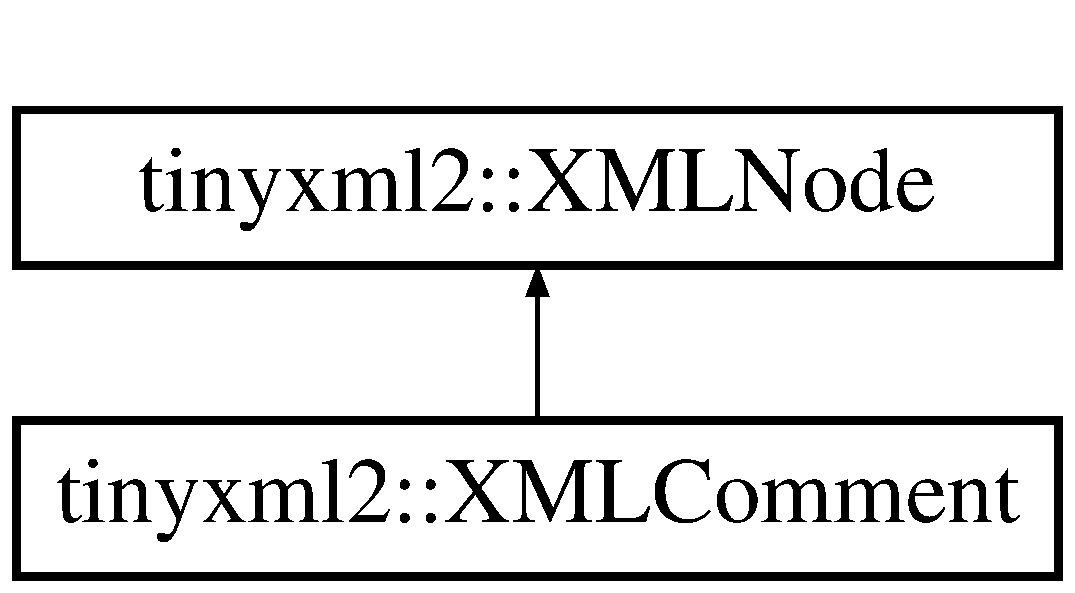
\includegraphics[height=2.000000cm]{classtinyxml2_1_1_x_m_l_comment}
\end{center}
\end{figure}
\subsection*{Public Member Functions}
\begin{DoxyCompactItemize}
\item 
\hypertarget{classtinyxml2_1_1_x_m_l_comment_a8093e1dc8a34fa446d9dc3fde0e6c0ee}{virtual \hyperlink{classtinyxml2_1_1_x_m_l_comment}{X\-M\-L\-Comment} $\ast$ \hyperlink{classtinyxml2_1_1_x_m_l_comment_a8093e1dc8a34fa446d9dc3fde0e6c0ee}{To\-Comment} ()}\label{classtinyxml2_1_1_x_m_l_comment_a8093e1dc8a34fa446d9dc3fde0e6c0ee}

\begin{DoxyCompactList}\small\item\em Safely cast to a Comment, or null. \end{DoxyCompactList}\item 
\hypertarget{classtinyxml2_1_1_x_m_l_comment_a422aabac22de7d9c9cad130897dd8b1c}{virtual const \hyperlink{classtinyxml2_1_1_x_m_l_comment}{X\-M\-L\-Comment} $\ast$ {\bfseries To\-Comment} () const }\label{classtinyxml2_1_1_x_m_l_comment_a422aabac22de7d9c9cad130897dd8b1c}

\item 
virtual bool \hyperlink{classtinyxml2_1_1_x_m_l_comment_aa382b1be6a8b0650c16a2d88bb499335}{Accept} (\hyperlink{classtinyxml2_1_1_x_m_l_visitor}{X\-M\-L\-Visitor} $\ast$visitor) const 
\item 
\hypertarget{classtinyxml2_1_1_x_m_l_comment_aa6ab35c3bb1c1840371dc32a2040c57f}{char $\ast$ {\bfseries Parse\-Deep} (char $\ast$, \hyperlink{classtinyxml2_1_1_str_pair}{Str\-Pair} $\ast$end\-Tag)}\label{classtinyxml2_1_1_x_m_l_comment_aa6ab35c3bb1c1840371dc32a2040c57f}

\item 
virtual \hyperlink{classtinyxml2_1_1_x_m_l_node}{X\-M\-L\-Node} $\ast$ \hyperlink{classtinyxml2_1_1_x_m_l_comment_a90bb60193a691b484f5e1b487857016d}{Shallow\-Clone} (\hyperlink{classtinyxml2_1_1_x_m_l_document}{X\-M\-L\-Document} $\ast$document) const 
\item 
virtual bool \hyperlink{classtinyxml2_1_1_x_m_l_comment_a2d9f26757b0018fce933e74420cda22a}{Shallow\-Equal} (const \hyperlink{classtinyxml2_1_1_x_m_l_node}{X\-M\-L\-Node} $\ast$compare) const 
\end{DoxyCompactItemize}
\subsection*{Protected Member Functions}
\begin{DoxyCompactItemize}
\item 
\hypertarget{classtinyxml2_1_1_x_m_l_comment_ae6463adc3edd93a8e5a9b2b7e99cdf91}{{\bfseries X\-M\-L\-Comment} (\hyperlink{classtinyxml2_1_1_x_m_l_document}{X\-M\-L\-Document} $\ast$doc)}\label{classtinyxml2_1_1_x_m_l_comment_ae6463adc3edd93a8e5a9b2b7e99cdf91}

\item 
\hypertarget{classtinyxml2_1_1_x_m_l_comment_aa0a9aae0850ac0e70d3cd20f6cb44447}{{\bfseries X\-M\-L\-Comment} (const \hyperlink{classtinyxml2_1_1_x_m_l_comment}{X\-M\-L\-Comment} \&)}\label{classtinyxml2_1_1_x_m_l_comment_aa0a9aae0850ac0e70d3cd20f6cb44447}

\item 
\hypertarget{classtinyxml2_1_1_x_m_l_comment_ac8de55f8381d110740772e6bf6f5755a}{\hyperlink{classtinyxml2_1_1_x_m_l_comment}{X\-M\-L\-Comment} \& {\bfseries operator=} (const \hyperlink{classtinyxml2_1_1_x_m_l_comment}{X\-M\-L\-Comment} \&)}\label{classtinyxml2_1_1_x_m_l_comment_ac8de55f8381d110740772e6bf6f5755a}

\end{DoxyCompactItemize}
\subsection*{Friends}
\begin{DoxyCompactItemize}
\item 
\hypertarget{classtinyxml2_1_1_x_m_l_comment_a4eee3bda60c60a30e4e8cd4ea91c4c6e}{class {\bfseries X\-M\-L\-Document}}\label{classtinyxml2_1_1_x_m_l_comment_a4eee3bda60c60a30e4e8cd4ea91c4c6e}

\end{DoxyCompactItemize}
\subsection*{Additional Inherited Members}


\subsection{Detailed Description}
An X\-M\-L Comment. 

\subsection{Member Function Documentation}
\hypertarget{classtinyxml2_1_1_x_m_l_comment_aa382b1be6a8b0650c16a2d88bb499335}{\index{tinyxml2\-::\-X\-M\-L\-Comment@{tinyxml2\-::\-X\-M\-L\-Comment}!Accept@{Accept}}
\index{Accept@{Accept}!tinyxml2::XMLComment@{tinyxml2\-::\-X\-M\-L\-Comment}}
\subsubsection[{Accept}]{\setlength{\rightskip}{0pt plus 5cm}bool tinyxml2\-::\-X\-M\-L\-Comment\-::\-Accept (
\begin{DoxyParamCaption}
\item[{{\bf X\-M\-L\-Visitor} $\ast$}]{visitor}
\end{DoxyParamCaption}
) const\hspace{0.3cm}{\ttfamily [virtual]}}}\label{classtinyxml2_1_1_x_m_l_comment_aa382b1be6a8b0650c16a2d88bb499335}
Accept a hierarchical visit of the nodes in the Tiny\-X\-M\-L-\/2 D\-O\-M. Every node in the X\-M\-L tree will be conditionally visited and the host will be called back via the \hyperlink{classtinyxml2_1_1_x_m_l_visitor}{X\-M\-L\-Visitor} interface.

This is essentially a S\-A\-X interface for Tiny\-X\-M\-L-\/2. (Note however it doesn't re-\/parse the X\-M\-L for the callbacks, so the performance of Tiny\-X\-M\-L-\/2 is unchanged by using this interface versus any other.)

The interface has been based on ideas from\-:


\begin{DoxyItemize}
\item \href{http://www.saxproject.org/}{\tt http\-://www.\-saxproject.\-org/}
\item \href{http://c2.com/cgi/wiki?HierarchicalVisitorPattern}{\tt http\-://c2.\-com/cgi/wiki?\-Hierarchical\-Visitor\-Pattern}
\end{DoxyItemize}

Which are both good references for \char`\"{}visiting\char`\"{}.

An example of using \hyperlink{classtinyxml2_1_1_x_m_l_comment_aa382b1be6a8b0650c16a2d88bb499335}{Accept()}\-: \begin{DoxyVerb}XMLPrinter printer;
tinyxmlDoc.Accept( &printer );
const char* xmlcstr = printer.CStr();
\end{DoxyVerb}
 

Implements \hyperlink{classtinyxml2_1_1_x_m_l_node_a81e66df0a44c67a7af17f3b77a152785}{tinyxml2\-::\-X\-M\-L\-Node}.

\hypertarget{classtinyxml2_1_1_x_m_l_comment_a90bb60193a691b484f5e1b487857016d}{\index{tinyxml2\-::\-X\-M\-L\-Comment@{tinyxml2\-::\-X\-M\-L\-Comment}!Shallow\-Clone@{Shallow\-Clone}}
\index{Shallow\-Clone@{Shallow\-Clone}!tinyxml2::XMLComment@{tinyxml2\-::\-X\-M\-L\-Comment}}
\subsubsection[{Shallow\-Clone}]{\setlength{\rightskip}{0pt plus 5cm}{\bf X\-M\-L\-Node} $\ast$ tinyxml2\-::\-X\-M\-L\-Comment\-::\-Shallow\-Clone (
\begin{DoxyParamCaption}
\item[{{\bf X\-M\-L\-Document} $\ast$}]{document}
\end{DoxyParamCaption}
) const\hspace{0.3cm}{\ttfamily [virtual]}}}\label{classtinyxml2_1_1_x_m_l_comment_a90bb60193a691b484f5e1b487857016d}
Make a copy of this node, but not its children. You may pass in a Document pointer that will be the owner of the new Node. If the 'document' is null, then the node returned will be allocated from the current Document. (this-\/$>$\hyperlink{classtinyxml2_1_1_x_m_l_node_af343d1ef0b45c0020e62d784d7e67a68}{Get\-Document()})

Note\-: if called on a \hyperlink{classtinyxml2_1_1_x_m_l_document}{X\-M\-L\-Document}, this will return null. 

Implements \hyperlink{classtinyxml2_1_1_x_m_l_node_a8402cbd3129d20e9e6024bbcc0531283}{tinyxml2\-::\-X\-M\-L\-Node}.

\hypertarget{classtinyxml2_1_1_x_m_l_comment_a2d9f26757b0018fce933e74420cda22a}{\index{tinyxml2\-::\-X\-M\-L\-Comment@{tinyxml2\-::\-X\-M\-L\-Comment}!Shallow\-Equal@{Shallow\-Equal}}
\index{Shallow\-Equal@{Shallow\-Equal}!tinyxml2::XMLComment@{tinyxml2\-::\-X\-M\-L\-Comment}}
\subsubsection[{Shallow\-Equal}]{\setlength{\rightskip}{0pt plus 5cm}bool tinyxml2\-::\-X\-M\-L\-Comment\-::\-Shallow\-Equal (
\begin{DoxyParamCaption}
\item[{const {\bf X\-M\-L\-Node} $\ast$}]{compare}
\end{DoxyParamCaption}
) const\hspace{0.3cm}{\ttfamily [virtual]}}}\label{classtinyxml2_1_1_x_m_l_comment_a2d9f26757b0018fce933e74420cda22a}
Test if 2 nodes are the same, but don't test children. The 2 nodes do not need to be in the same Document.

Note\-: if called on a \hyperlink{classtinyxml2_1_1_x_m_l_document}{X\-M\-L\-Document}, this will return false. 

Implements \hyperlink{classtinyxml2_1_1_x_m_l_node_a7ce18b751c3ea09eac292dca264f9226}{tinyxml2\-::\-X\-M\-L\-Node}.



The documentation for this class was generated from the following files\-:\begin{DoxyCompactItemize}
\item 
Joes\-\_\-\-S\-D\-L\-\_\-\-Framework/tinyxml2.\-h\item 
Joes\-\_\-\-S\-D\-L\-\_\-\-Framework/tinyxml2.\-cpp\end{DoxyCompactItemize}

\hypertarget{classtinyxml2_1_1_x_m_l_const_handle}{\section{tinyxml2\-:\-:X\-M\-L\-Const\-Handle Class Reference}
\label{classtinyxml2_1_1_x_m_l_const_handle}\index{tinyxml2\-::\-X\-M\-L\-Const\-Handle@{tinyxml2\-::\-X\-M\-L\-Const\-Handle}}
}


{\ttfamily \#include $<$tinyxml2.\-h$>$}

\subsection*{Public Member Functions}
\begin{DoxyCompactItemize}
\item 
\hypertarget{classtinyxml2_1_1_x_m_l_const_handle_a098bda71fa11d7c74ccddab59d5dd534}{{\bfseries X\-M\-L\-Const\-Handle} (const \hyperlink{classtinyxml2_1_1_x_m_l_node}{X\-M\-L\-Node} $\ast$node)}\label{classtinyxml2_1_1_x_m_l_const_handle_a098bda71fa11d7c74ccddab59d5dd534}

\item 
\hypertarget{classtinyxml2_1_1_x_m_l_const_handle_a8420a0c4720637e0529e78c2e22f2b0b}{{\bfseries X\-M\-L\-Const\-Handle} (const \hyperlink{classtinyxml2_1_1_x_m_l_node}{X\-M\-L\-Node} \&node)}\label{classtinyxml2_1_1_x_m_l_const_handle_a8420a0c4720637e0529e78c2e22f2b0b}

\item 
\hypertarget{classtinyxml2_1_1_x_m_l_const_handle_a639317ad315ff24f4ef0dc69312d7303}{{\bfseries X\-M\-L\-Const\-Handle} (const \hyperlink{classtinyxml2_1_1_x_m_l_const_handle}{X\-M\-L\-Const\-Handle} \&ref)}\label{classtinyxml2_1_1_x_m_l_const_handle_a639317ad315ff24f4ef0dc69312d7303}

\item 
\hypertarget{classtinyxml2_1_1_x_m_l_const_handle_a2d74c91df1ff9aa5f9b57e3dceddbf94}{\hyperlink{classtinyxml2_1_1_x_m_l_const_handle}{X\-M\-L\-Const\-Handle} \& {\bfseries operator=} (const \hyperlink{classtinyxml2_1_1_x_m_l_const_handle}{X\-M\-L\-Const\-Handle} \&ref)}\label{classtinyxml2_1_1_x_m_l_const_handle_a2d74c91df1ff9aa5f9b57e3dceddbf94}

\item 
\hypertarget{classtinyxml2_1_1_x_m_l_const_handle_a64c4ff7074effc1fd181d68d23f9d1e4}{const \hyperlink{classtinyxml2_1_1_x_m_l_const_handle}{X\-M\-L\-Const\-Handle} {\bfseries First\-Child} () const }\label{classtinyxml2_1_1_x_m_l_const_handle_a64c4ff7074effc1fd181d68d23f9d1e4}

\item 
\hypertarget{classtinyxml2_1_1_x_m_l_const_handle_a5c197d0b57f8e560d93356a4a281469c}{const \hyperlink{classtinyxml2_1_1_x_m_l_const_handle}{X\-M\-L\-Const\-Handle} {\bfseries First\-Child\-Element} (const char $\ast$value=0) const }\label{classtinyxml2_1_1_x_m_l_const_handle_a5c197d0b57f8e560d93356a4a281469c}

\item 
\hypertarget{classtinyxml2_1_1_x_m_l_const_handle_afec9a68e7951193bc5a6e876d602f263}{const \hyperlink{classtinyxml2_1_1_x_m_l_const_handle}{X\-M\-L\-Const\-Handle} {\bfseries Last\-Child} () const }\label{classtinyxml2_1_1_x_m_l_const_handle_afec9a68e7951193bc5a6e876d602f263}

\item 
\hypertarget{classtinyxml2_1_1_x_m_l_const_handle_a1c400e66dace6fdab4927adb21090059}{const \hyperlink{classtinyxml2_1_1_x_m_l_const_handle}{X\-M\-L\-Const\-Handle} {\bfseries Last\-Child\-Element} (const char $\ast$\-\_\-value=0) const }\label{classtinyxml2_1_1_x_m_l_const_handle_a1c400e66dace6fdab4927adb21090059}

\item 
\hypertarget{classtinyxml2_1_1_x_m_l_const_handle_a6917564e26b2c20ebdcb23c7940ad80a}{const \hyperlink{classtinyxml2_1_1_x_m_l_const_handle}{X\-M\-L\-Const\-Handle} {\bfseries Previous\-Sibling} () const }\label{classtinyxml2_1_1_x_m_l_const_handle_a6917564e26b2c20ebdcb23c7940ad80a}

\item 
\hypertarget{classtinyxml2_1_1_x_m_l_const_handle_acb2e1c5762eff9f6ed72d1a2dfc14271}{const \hyperlink{classtinyxml2_1_1_x_m_l_const_handle}{X\-M\-L\-Const\-Handle} {\bfseries Previous\-Sibling\-Element} (const char $\ast$\-\_\-value=0) const }\label{classtinyxml2_1_1_x_m_l_const_handle_acb2e1c5762eff9f6ed72d1a2dfc14271}

\item 
\hypertarget{classtinyxml2_1_1_x_m_l_const_handle_a596e248c8014d718f41658502a2e221b}{const \hyperlink{classtinyxml2_1_1_x_m_l_const_handle}{X\-M\-L\-Const\-Handle} {\bfseries Next\-Sibling} () const }\label{classtinyxml2_1_1_x_m_l_const_handle_a596e248c8014d718f41658502a2e221b}

\item 
\hypertarget{classtinyxml2_1_1_x_m_l_const_handle_a3bbdd3d866c750473bd69a232704503b}{const \hyperlink{classtinyxml2_1_1_x_m_l_const_handle}{X\-M\-L\-Const\-Handle} {\bfseries Next\-Sibling\-Element} (const char $\ast$\-\_\-value=0) const }\label{classtinyxml2_1_1_x_m_l_const_handle_a3bbdd3d866c750473bd69a232704503b}

\item 
\hypertarget{classtinyxml2_1_1_x_m_l_const_handle_a95d0256318c10c3f75fa5f8ffb3e4bc1}{const \hyperlink{classtinyxml2_1_1_x_m_l_node}{X\-M\-L\-Node} $\ast$ {\bfseries To\-Node} () const }\label{classtinyxml2_1_1_x_m_l_const_handle_a95d0256318c10c3f75fa5f8ffb3e4bc1}

\item 
\hypertarget{classtinyxml2_1_1_x_m_l_const_handle_a5a48adefc2a5e70d4ce5b55692a0e2f9}{const \hyperlink{classtinyxml2_1_1_x_m_l_element}{X\-M\-L\-Element} $\ast$ {\bfseries To\-Element} () const }\label{classtinyxml2_1_1_x_m_l_const_handle_a5a48adefc2a5e70d4ce5b55692a0e2f9}

\item 
\hypertarget{classtinyxml2_1_1_x_m_l_const_handle_ad86ca7dbb20d0495ae357fe7a866e0be}{const \hyperlink{classtinyxml2_1_1_x_m_l_text}{X\-M\-L\-Text} $\ast$ {\bfseries To\-Text} () const }\label{classtinyxml2_1_1_x_m_l_const_handle_ad86ca7dbb20d0495ae357fe7a866e0be}

\item 
\hypertarget{classtinyxml2_1_1_x_m_l_const_handle_acb358a329e54fa204ed2d0b181566828}{const \hyperlink{classtinyxml2_1_1_x_m_l_unknown}{X\-M\-L\-Unknown} $\ast$ {\bfseries To\-Unknown} () const }\label{classtinyxml2_1_1_x_m_l_const_handle_acb358a329e54fa204ed2d0b181566828}

\item 
\hypertarget{classtinyxml2_1_1_x_m_l_const_handle_a5de0c175845bc30a6f9b3d88d8877eaf}{const \hyperlink{classtinyxml2_1_1_x_m_l_declaration}{X\-M\-L\-Declaration} $\ast$ {\bfseries To\-Declaration} () const }\label{classtinyxml2_1_1_x_m_l_const_handle_a5de0c175845bc30a6f9b3d88d8877eaf}

\end{DoxyCompactItemize}


\subsection{Detailed Description}
A variant of the \hyperlink{classtinyxml2_1_1_x_m_l_handle}{X\-M\-L\-Handle} class for working with const X\-M\-L\-Nodes and Documents. It is the same in all regards, except for the 'const' qualifiers. See \hyperlink{classtinyxml2_1_1_x_m_l_handle}{X\-M\-L\-Handle} for A\-P\-I. 

The documentation for this class was generated from the following file\-:\begin{DoxyCompactItemize}
\item 
Joes\-\_\-\-S\-D\-L\-\_\-\-Framework/tinyxml2.\-h\end{DoxyCompactItemize}

\hypertarget{classtinyxml2_1_1_x_m_l_declaration}{\section{tinyxml2\-:\-:X\-M\-L\-Declaration Class Reference}
\label{classtinyxml2_1_1_x_m_l_declaration}\index{tinyxml2\-::\-X\-M\-L\-Declaration@{tinyxml2\-::\-X\-M\-L\-Declaration}}
}


{\ttfamily \#include $<$tinyxml2.\-h$>$}

Inheritance diagram for tinyxml2\-:\-:X\-M\-L\-Declaration\-:\begin{figure}[H]
\begin{center}
\leavevmode
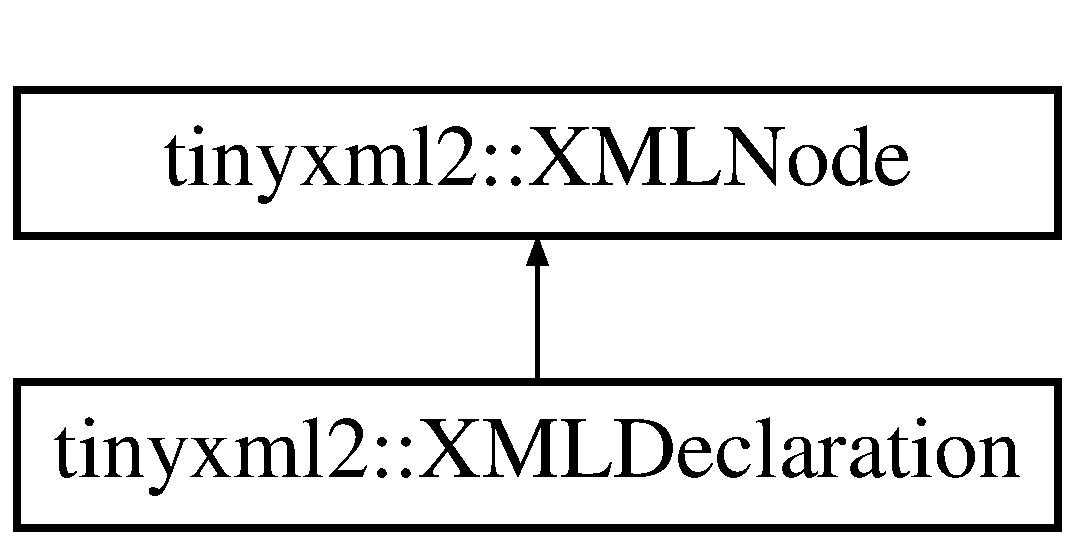
\includegraphics[height=2.000000cm]{classtinyxml2_1_1_x_m_l_declaration}
\end{center}
\end{figure}
\subsection*{Public Member Functions}
\begin{DoxyCompactItemize}
\item 
virtual \hyperlink{classtinyxml2_1_1_x_m_l_declaration}{X\-M\-L\-Declaration} $\ast$ \hyperlink{classtinyxml2_1_1_x_m_l_declaration_a159d8ac45865215e88059ea1e5b52fc5}{To\-Declaration} ()
\begin{DoxyCompactList}\small\item\em Safely cast to a Declaration, or null. \end{DoxyCompactList}\item 
virtual const \hyperlink{classtinyxml2_1_1_x_m_l_declaration}{X\-M\-L\-Declaration} $\ast$ \hyperlink{classtinyxml2_1_1_x_m_l_declaration_af724607a5fa810496fd6a21f5975a643}{To\-Declaration} () const 
\item 
virtual bool \hyperlink{classtinyxml2_1_1_x_m_l_declaration_a953a7359cc312d15218eb5843a4ca108}{Accept} (\hyperlink{classtinyxml2_1_1_x_m_l_visitor}{X\-M\-L\-Visitor} $\ast$visitor) const 
\item 
char $\ast$ \hyperlink{classtinyxml2_1_1_x_m_l_declaration_a19e33e0a9f9500f449261558c36f9a44}{Parse\-Deep} (char $\ast$, \hyperlink{classtinyxml2_1_1_str_pair}{Str\-Pair} $\ast$end\-Tag)
\item 
virtual \hyperlink{classtinyxml2_1_1_x_m_l_node}{X\-M\-L\-Node} $\ast$ \hyperlink{classtinyxml2_1_1_x_m_l_declaration_a39458732ee6796cfc85dd35d3c488e0b}{Shallow\-Clone} (\hyperlink{classtinyxml2_1_1_x_m_l_document}{X\-M\-L\-Document} $\ast$document) const 
\item 
virtual bool \hyperlink{classtinyxml2_1_1_x_m_l_declaration_ace0d2d9bc1b63278bd5e984ebe0c7bd0}{Shallow\-Equal} (const \hyperlink{classtinyxml2_1_1_x_m_l_node}{X\-M\-L\-Node} $\ast$compare) const 
\end{DoxyCompactItemize}
\subsection*{Protected Member Functions}
\begin{DoxyCompactItemize}
\item 
\hyperlink{classtinyxml2_1_1_x_m_l_declaration_aef9586f2ce5df5feba74dde49a242b06}{X\-M\-L\-Declaration} (\hyperlink{classtinyxml2_1_1_x_m_l_document}{X\-M\-L\-Document} $\ast$doc)
\item 
virtual \hyperlink{classtinyxml2_1_1_x_m_l_declaration_ab93d5bf4f5d58b4144963cf739cf6dcc}{$\sim$\-X\-M\-L\-Declaration} ()
\item 
\hyperlink{classtinyxml2_1_1_x_m_l_declaration_a5229cc0b31f034f93289af27ec3e2836}{X\-M\-L\-Declaration} (const \hyperlink{classtinyxml2_1_1_x_m_l_declaration}{X\-M\-L\-Declaration} \&)
\item 
\hyperlink{classtinyxml2_1_1_x_m_l_declaration}{X\-M\-L\-Declaration} \& \hyperlink{classtinyxml2_1_1_x_m_l_declaration_a79eb518c2c2b1b99a122a5d5a308b7ee}{operator=} (const \hyperlink{classtinyxml2_1_1_x_m_l_declaration}{X\-M\-L\-Declaration} \&)
\end{DoxyCompactItemize}
\subsection*{Friends}
\begin{DoxyCompactItemize}
\item 
class \hyperlink{classtinyxml2_1_1_x_m_l_declaration_a4eee3bda60c60a30e4e8cd4ea91c4c6e}{X\-M\-L\-Document}
\end{DoxyCompactItemize}
\subsection*{Additional Inherited Members}


\subsection{Detailed Description}
In correct X\-M\-L the declaration is the first entry in the file. \begin{DoxyVerb}    <?xml version="1.0" standalone="yes"?>
\end{DoxyVerb}


Tiny\-X\-M\-L-\/2 will happily read or write files without a declaration, however.

The text of the declaration isn't interpreted. It is parsed and written as a string. 

\subsection{Constructor \& Destructor Documentation}
\hypertarget{classtinyxml2_1_1_x_m_l_declaration_aef9586f2ce5df5feba74dde49a242b06}{\index{tinyxml2\-::\-X\-M\-L\-Declaration@{tinyxml2\-::\-X\-M\-L\-Declaration}!X\-M\-L\-Declaration@{X\-M\-L\-Declaration}}
\index{X\-M\-L\-Declaration@{X\-M\-L\-Declaration}!tinyxml2::XMLDeclaration@{tinyxml2\-::\-X\-M\-L\-Declaration}}
\subsubsection[{X\-M\-L\-Declaration}]{\setlength{\rightskip}{0pt plus 5cm}tinyxml2\-::\-X\-M\-L\-Declaration\-::\-X\-M\-L\-Declaration (
\begin{DoxyParamCaption}
\item[{{\bf X\-M\-L\-Document} $\ast$}]{doc}
\end{DoxyParamCaption}
)\hspace{0.3cm}{\ttfamily [protected]}}}\label{classtinyxml2_1_1_x_m_l_declaration_aef9586f2ce5df5feba74dde49a242b06}
\hypertarget{classtinyxml2_1_1_x_m_l_declaration_ab93d5bf4f5d58b4144963cf739cf6dcc}{\index{tinyxml2\-::\-X\-M\-L\-Declaration@{tinyxml2\-::\-X\-M\-L\-Declaration}!$\sim$\-X\-M\-L\-Declaration@{$\sim$\-X\-M\-L\-Declaration}}
\index{$\sim$\-X\-M\-L\-Declaration@{$\sim$\-X\-M\-L\-Declaration}!tinyxml2::XMLDeclaration@{tinyxml2\-::\-X\-M\-L\-Declaration}}
\subsubsection[{$\sim$\-X\-M\-L\-Declaration}]{\setlength{\rightskip}{0pt plus 5cm}tinyxml2\-::\-X\-M\-L\-Declaration\-::$\sim$\-X\-M\-L\-Declaration (
\begin{DoxyParamCaption}
{}
\end{DoxyParamCaption}
)\hspace{0.3cm}{\ttfamily [protected]}, {\ttfamily [virtual]}}}\label{classtinyxml2_1_1_x_m_l_declaration_ab93d5bf4f5d58b4144963cf739cf6dcc}
\hypertarget{classtinyxml2_1_1_x_m_l_declaration_a5229cc0b31f034f93289af27ec3e2836}{\index{tinyxml2\-::\-X\-M\-L\-Declaration@{tinyxml2\-::\-X\-M\-L\-Declaration}!X\-M\-L\-Declaration@{X\-M\-L\-Declaration}}
\index{X\-M\-L\-Declaration@{X\-M\-L\-Declaration}!tinyxml2::XMLDeclaration@{tinyxml2\-::\-X\-M\-L\-Declaration}}
\subsubsection[{X\-M\-L\-Declaration}]{\setlength{\rightskip}{0pt plus 5cm}tinyxml2\-::\-X\-M\-L\-Declaration\-::\-X\-M\-L\-Declaration (
\begin{DoxyParamCaption}
\item[{const {\bf X\-M\-L\-Declaration} \&}]{}
\end{DoxyParamCaption}
)\hspace{0.3cm}{\ttfamily [protected]}}}\label{classtinyxml2_1_1_x_m_l_declaration_a5229cc0b31f034f93289af27ec3e2836}


\subsection{Member Function Documentation}
\hypertarget{classtinyxml2_1_1_x_m_l_declaration_a953a7359cc312d15218eb5843a4ca108}{\index{tinyxml2\-::\-X\-M\-L\-Declaration@{tinyxml2\-::\-X\-M\-L\-Declaration}!Accept@{Accept}}
\index{Accept@{Accept}!tinyxml2::XMLDeclaration@{tinyxml2\-::\-X\-M\-L\-Declaration}}
\subsubsection[{Accept}]{\setlength{\rightskip}{0pt plus 5cm}bool tinyxml2\-::\-X\-M\-L\-Declaration\-::\-Accept (
\begin{DoxyParamCaption}
\item[{{\bf X\-M\-L\-Visitor} $\ast$}]{visitor}
\end{DoxyParamCaption}
) const\hspace{0.3cm}{\ttfamily [virtual]}}}\label{classtinyxml2_1_1_x_m_l_declaration_a953a7359cc312d15218eb5843a4ca108}
Accept a hierarchical visit of the nodes in the Tiny\-X\-M\-L-\/2 D\-O\-M. Every node in the X\-M\-L tree will be conditionally visited and the host will be called back via the \hyperlink{classtinyxml2_1_1_x_m_l_visitor}{X\-M\-L\-Visitor} interface.

This is essentially a S\-A\-X interface for Tiny\-X\-M\-L-\/2. (Note however it doesn't re-\/parse the X\-M\-L for the callbacks, so the performance of Tiny\-X\-M\-L-\/2 is unchanged by using this interface versus any other.)

The interface has been based on ideas from\-:


\begin{DoxyItemize}
\item \href{http://www.saxproject.org/}{\tt http\-://www.\-saxproject.\-org/}
\item \href{http://c2.com/cgi/wiki?HierarchicalVisitorPattern}{\tt http\-://c2.\-com/cgi/wiki?\-Hierarchical\-Visitor\-Pattern}
\end{DoxyItemize}

Which are both good references for \char`\"{}visiting\char`\"{}.

An example of using \hyperlink{classtinyxml2_1_1_x_m_l_declaration_a953a7359cc312d15218eb5843a4ca108}{Accept()}\-: \begin{DoxyVerb}XMLPrinter printer;
tinyxmlDoc.Accept( &printer );
const char* xmlcstr = printer.CStr();
\end{DoxyVerb}
 

Implements \hyperlink{classtinyxml2_1_1_x_m_l_node_a81e66df0a44c67a7af17f3b77a152785}{tinyxml2\-::\-X\-M\-L\-Node}.

\hypertarget{classtinyxml2_1_1_x_m_l_declaration_a79eb518c2c2b1b99a122a5d5a308b7ee}{\index{tinyxml2\-::\-X\-M\-L\-Declaration@{tinyxml2\-::\-X\-M\-L\-Declaration}!operator=@{operator=}}
\index{operator=@{operator=}!tinyxml2::XMLDeclaration@{tinyxml2\-::\-X\-M\-L\-Declaration}}
\subsubsection[{operator=}]{\setlength{\rightskip}{0pt plus 5cm}{\bf X\-M\-L\-Declaration}\& tinyxml2\-::\-X\-M\-L\-Declaration\-::operator= (
\begin{DoxyParamCaption}
\item[{const {\bf X\-M\-L\-Declaration} \&}]{}
\end{DoxyParamCaption}
)\hspace{0.3cm}{\ttfamily [protected]}}}\label{classtinyxml2_1_1_x_m_l_declaration_a79eb518c2c2b1b99a122a5d5a308b7ee}
\hypertarget{classtinyxml2_1_1_x_m_l_declaration_a19e33e0a9f9500f449261558c36f9a44}{\index{tinyxml2\-::\-X\-M\-L\-Declaration@{tinyxml2\-::\-X\-M\-L\-Declaration}!Parse\-Deep@{Parse\-Deep}}
\index{Parse\-Deep@{Parse\-Deep}!tinyxml2::XMLDeclaration@{tinyxml2\-::\-X\-M\-L\-Declaration}}
\subsubsection[{Parse\-Deep}]{\setlength{\rightskip}{0pt plus 5cm}char $\ast$ tinyxml2\-::\-X\-M\-L\-Declaration\-::\-Parse\-Deep (
\begin{DoxyParamCaption}
\item[{char $\ast$}]{p, }
\item[{{\bf Str\-Pair} $\ast$}]{end\-Tag}
\end{DoxyParamCaption}
)\hspace{0.3cm}{\ttfamily [virtual]}}}\label{classtinyxml2_1_1_x_m_l_declaration_a19e33e0a9f9500f449261558c36f9a44}


Reimplemented from \hyperlink{classtinyxml2_1_1_x_m_l_node_a7610d0f603e8b603d2078521811a23c1}{tinyxml2\-::\-X\-M\-L\-Node}.

\hypertarget{classtinyxml2_1_1_x_m_l_declaration_a39458732ee6796cfc85dd35d3c488e0b}{\index{tinyxml2\-::\-X\-M\-L\-Declaration@{tinyxml2\-::\-X\-M\-L\-Declaration}!Shallow\-Clone@{Shallow\-Clone}}
\index{Shallow\-Clone@{Shallow\-Clone}!tinyxml2::XMLDeclaration@{tinyxml2\-::\-X\-M\-L\-Declaration}}
\subsubsection[{Shallow\-Clone}]{\setlength{\rightskip}{0pt plus 5cm}{\bf X\-M\-L\-Node} $\ast$ tinyxml2\-::\-X\-M\-L\-Declaration\-::\-Shallow\-Clone (
\begin{DoxyParamCaption}
\item[{{\bf X\-M\-L\-Document} $\ast$}]{document}
\end{DoxyParamCaption}
) const\hspace{0.3cm}{\ttfamily [virtual]}}}\label{classtinyxml2_1_1_x_m_l_declaration_a39458732ee6796cfc85dd35d3c488e0b}
Make a copy of this node, but not its children. You may pass in a Document pointer that will be the owner of the new Node. If the 'document' is null, then the node returned will be allocated from the current Document. (this-\/$>$\hyperlink{classtinyxml2_1_1_x_m_l_node_af343d1ef0b45c0020e62d784d7e67a68}{Get\-Document()})

Note\-: if called on a \hyperlink{classtinyxml2_1_1_x_m_l_document}{X\-M\-L\-Document}, this will return null. 

Implements \hyperlink{classtinyxml2_1_1_x_m_l_node_a8402cbd3129d20e9e6024bbcc0531283}{tinyxml2\-::\-X\-M\-L\-Node}.

\hypertarget{classtinyxml2_1_1_x_m_l_declaration_ace0d2d9bc1b63278bd5e984ebe0c7bd0}{\index{tinyxml2\-::\-X\-M\-L\-Declaration@{tinyxml2\-::\-X\-M\-L\-Declaration}!Shallow\-Equal@{Shallow\-Equal}}
\index{Shallow\-Equal@{Shallow\-Equal}!tinyxml2::XMLDeclaration@{tinyxml2\-::\-X\-M\-L\-Declaration}}
\subsubsection[{Shallow\-Equal}]{\setlength{\rightskip}{0pt plus 5cm}bool tinyxml2\-::\-X\-M\-L\-Declaration\-::\-Shallow\-Equal (
\begin{DoxyParamCaption}
\item[{const {\bf X\-M\-L\-Node} $\ast$}]{compare}
\end{DoxyParamCaption}
) const\hspace{0.3cm}{\ttfamily [virtual]}}}\label{classtinyxml2_1_1_x_m_l_declaration_ace0d2d9bc1b63278bd5e984ebe0c7bd0}
Test if 2 nodes are the same, but don't test children. The 2 nodes do not need to be in the same Document.

Note\-: if called on a \hyperlink{classtinyxml2_1_1_x_m_l_document}{X\-M\-L\-Document}, this will return false. 

Implements \hyperlink{classtinyxml2_1_1_x_m_l_node_a7ce18b751c3ea09eac292dca264f9226}{tinyxml2\-::\-X\-M\-L\-Node}.

\hypertarget{classtinyxml2_1_1_x_m_l_declaration_a159d8ac45865215e88059ea1e5b52fc5}{\index{tinyxml2\-::\-X\-M\-L\-Declaration@{tinyxml2\-::\-X\-M\-L\-Declaration}!To\-Declaration@{To\-Declaration}}
\index{To\-Declaration@{To\-Declaration}!tinyxml2::XMLDeclaration@{tinyxml2\-::\-X\-M\-L\-Declaration}}
\subsubsection[{To\-Declaration}]{\setlength{\rightskip}{0pt plus 5cm}virtual {\bf X\-M\-L\-Declaration}$\ast$ tinyxml2\-::\-X\-M\-L\-Declaration\-::\-To\-Declaration (
\begin{DoxyParamCaption}
{}
\end{DoxyParamCaption}
)\hspace{0.3cm}{\ttfamily [inline]}, {\ttfamily [virtual]}}}\label{classtinyxml2_1_1_x_m_l_declaration_a159d8ac45865215e88059ea1e5b52fc5}


Safely cast to a Declaration, or null. 



Reimplemented from \hyperlink{classtinyxml2_1_1_x_m_l_node_a174fd4c22c010b58138c1b84a0dfbd51}{tinyxml2\-::\-X\-M\-L\-Node}.

\hypertarget{classtinyxml2_1_1_x_m_l_declaration_af724607a5fa810496fd6a21f5975a643}{\index{tinyxml2\-::\-X\-M\-L\-Declaration@{tinyxml2\-::\-X\-M\-L\-Declaration}!To\-Declaration@{To\-Declaration}}
\index{To\-Declaration@{To\-Declaration}!tinyxml2::XMLDeclaration@{tinyxml2\-::\-X\-M\-L\-Declaration}}
\subsubsection[{To\-Declaration}]{\setlength{\rightskip}{0pt plus 5cm}virtual const {\bf X\-M\-L\-Declaration}$\ast$ tinyxml2\-::\-X\-M\-L\-Declaration\-::\-To\-Declaration (
\begin{DoxyParamCaption}
{}
\end{DoxyParamCaption}
) const\hspace{0.3cm}{\ttfamily [inline]}, {\ttfamily [virtual]}}}\label{classtinyxml2_1_1_x_m_l_declaration_af724607a5fa810496fd6a21f5975a643}


Reimplemented from \hyperlink{classtinyxml2_1_1_x_m_l_node_aedae0bbb58d533a4b8a61042388b49e5}{tinyxml2\-::\-X\-M\-L\-Node}.



\subsection{Friends And Related Function Documentation}
\hypertarget{classtinyxml2_1_1_x_m_l_declaration_a4eee3bda60c60a30e4e8cd4ea91c4c6e}{\index{tinyxml2\-::\-X\-M\-L\-Declaration@{tinyxml2\-::\-X\-M\-L\-Declaration}!X\-M\-L\-Document@{X\-M\-L\-Document}}
\index{X\-M\-L\-Document@{X\-M\-L\-Document}!tinyxml2::XMLDeclaration@{tinyxml2\-::\-X\-M\-L\-Declaration}}
\subsubsection[{X\-M\-L\-Document}]{\setlength{\rightskip}{0pt plus 5cm}friend class {\bf X\-M\-L\-Document}\hspace{0.3cm}{\ttfamily [friend]}}}\label{classtinyxml2_1_1_x_m_l_declaration_a4eee3bda60c60a30e4e8cd4ea91c4c6e}


The documentation for this class was generated from the following files\-:\begin{DoxyCompactItemize}
\item 
Joes\-\_\-\-S\-D\-L\-\_\-\-Framework/\hyperlink{tinyxml2_8h}{tinyxml2.\-h}\item 
Joes\-\_\-\-S\-D\-L\-\_\-\-Framework/\hyperlink{tinyxml2_8cpp}{tinyxml2.\-cpp}\end{DoxyCompactItemize}

\hypertarget{classtinyxml2_1_1_x_m_l_document}{\section{tinyxml2\-:\-:X\-M\-L\-Document Class Reference}
\label{classtinyxml2_1_1_x_m_l_document}\index{tinyxml2\-::\-X\-M\-L\-Document@{tinyxml2\-::\-X\-M\-L\-Document}}
}


{\ttfamily \#include $<$tinyxml2.\-h$>$}

Inheritance diagram for tinyxml2\-:\-:X\-M\-L\-Document\-:\begin{figure}[H]
\begin{center}
\leavevmode
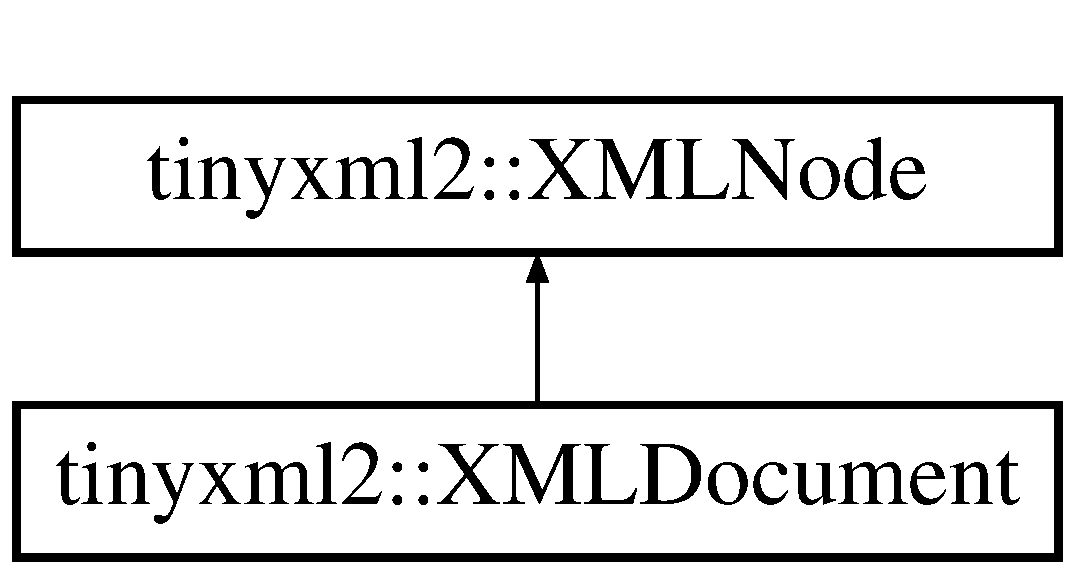
\includegraphics[height=2.000000cm]{classtinyxml2_1_1_x_m_l_document}
\end{center}
\end{figure}
\subsection*{Public Member Functions}
\begin{DoxyCompactItemize}
\item 
\hypertarget{classtinyxml2_1_1_x_m_l_document_af1574f76ebb619f25ef3f09eb2ba5188}{\hyperlink{classtinyxml2_1_1_x_m_l_document_af1574f76ebb619f25ef3f09eb2ba5188}{X\-M\-L\-Document} (bool process\-Entities=true, Whitespace=P\-R\-E\-S\-E\-R\-V\-E\-\_\-\-W\-H\-I\-T\-E\-S\-P\-A\-C\-E)}\label{classtinyxml2_1_1_x_m_l_document_af1574f76ebb619f25ef3f09eb2ba5188}

\begin{DoxyCompactList}\small\item\em constructor \end{DoxyCompactList}\item 
\hypertarget{classtinyxml2_1_1_x_m_l_document_a3e185f880882bd978367bb55937735ec}{virtual \hyperlink{classtinyxml2_1_1_x_m_l_document}{X\-M\-L\-Document} $\ast$ \hyperlink{classtinyxml2_1_1_x_m_l_document_a3e185f880882bd978367bb55937735ec}{To\-Document} ()}\label{classtinyxml2_1_1_x_m_l_document_a3e185f880882bd978367bb55937735ec}

\begin{DoxyCompactList}\small\item\em Safely cast to a Document, or null. \end{DoxyCompactList}\item 
\hypertarget{classtinyxml2_1_1_x_m_l_document_a15eb1a62afa18c66808031da647d1129}{virtual const \hyperlink{classtinyxml2_1_1_x_m_l_document}{X\-M\-L\-Document} $\ast$ {\bfseries To\-Document} () const }\label{classtinyxml2_1_1_x_m_l_document_a15eb1a62afa18c66808031da647d1129}

\item 
X\-M\-L\-Error \hyperlink{classtinyxml2_1_1_x_m_l_document_a1819bd34f540a7304c105a6232d25a1f}{Parse} (const char $\ast$xml, size\-\_\-t n\-Bytes=(size\-\_\-t)(-\/1))
\item 
X\-M\-L\-Error \hyperlink{classtinyxml2_1_1_x_m_l_document_a2ebd4647a8af5fc6831b294ac26a150a}{Load\-File} (const char $\ast$filename)
\item 
X\-M\-L\-Error \hyperlink{classtinyxml2_1_1_x_m_l_document_a5f1d330fad44c52f3d265338dd2a6dc2}{Load\-File} (F\-I\-L\-E $\ast$)
\item 
X\-M\-L\-Error \hyperlink{classtinyxml2_1_1_x_m_l_document_a73ac416b4a2aa0952e841220eb3da18f}{Save\-File} (const char $\ast$filename, bool compact=false)
\item 
X\-M\-L\-Error \hyperlink{classtinyxml2_1_1_x_m_l_document_a8b95779479a0035acc67b3a61dfe1b74}{Save\-File} (F\-I\-L\-E $\ast$fp, bool compact=false)
\item 
\hypertarget{classtinyxml2_1_1_x_m_l_document_adfcff7d0599cd520e9fcbb8891e1b678}{bool {\bfseries Process\-Entities} () const }\label{classtinyxml2_1_1_x_m_l_document_adfcff7d0599cd520e9fcbb8891e1b678}

\item 
\hypertarget{classtinyxml2_1_1_x_m_l_document_a94b3ea2f77c9ac831723984df5a02d01}{Whitespace {\bfseries Whitespace\-Mode} () const }\label{classtinyxml2_1_1_x_m_l_document_a94b3ea2f77c9ac831723984df5a02d01}

\item 
bool \hyperlink{classtinyxml2_1_1_x_m_l_document_a530649e9de7e5aa8df9c37f66197fcb6}{Has\-B\-O\-M} () const 
\item 
void \hyperlink{classtinyxml2_1_1_x_m_l_document_a14419b698f7c4b140df4e80f3f0c93b0}{Set\-B\-O\-M} (bool use\-B\-O\-M)
\item 
\hyperlink{classtinyxml2_1_1_x_m_l_element}{X\-M\-L\-Element} $\ast$ \hyperlink{classtinyxml2_1_1_x_m_l_document_ad2b70320d3c2a071c2f36928edff3e1c}{Root\-Element} ()
\item 
\hypertarget{classtinyxml2_1_1_x_m_l_document_a23a25b573d2adf3ee6075636c2a31c73}{const \hyperlink{classtinyxml2_1_1_x_m_l_element}{X\-M\-L\-Element} $\ast$ {\bfseries Root\-Element} () const }\label{classtinyxml2_1_1_x_m_l_document_a23a25b573d2adf3ee6075636c2a31c73}

\item 
void \hyperlink{classtinyxml2_1_1_x_m_l_document_a686ea28672c0e0c60383ec28148c1ac0}{Print} (\hyperlink{classtinyxml2_1_1_x_m_l_printer}{X\-M\-L\-Printer} $\ast$streamer=0) const 
\item 
virtual bool \hyperlink{classtinyxml2_1_1_x_m_l_document_aa08503d24898bf9992ae5e5fb8b0cf87}{Accept} (\hyperlink{classtinyxml2_1_1_x_m_l_visitor}{X\-M\-L\-Visitor} $\ast$visitor) const 
\item 
\hyperlink{classtinyxml2_1_1_x_m_l_element}{X\-M\-L\-Element} $\ast$ \hyperlink{classtinyxml2_1_1_x_m_l_document_a3c335a700a43d7c363a393142a23f234}{New\-Element} (const char $\ast$name)
\item 
\hyperlink{classtinyxml2_1_1_x_m_l_comment}{X\-M\-L\-Comment} $\ast$ \hyperlink{classtinyxml2_1_1_x_m_l_document_a386df0befd06aadb5e0cd21381aa955a}{New\-Comment} (const char $\ast$comment)
\item 
\hyperlink{classtinyxml2_1_1_x_m_l_text}{X\-M\-L\-Text} $\ast$ \hyperlink{classtinyxml2_1_1_x_m_l_document_acece5de77a0819f2341b08c1e1ed9987}{New\-Text} (const char $\ast$text)
\item 
\hyperlink{classtinyxml2_1_1_x_m_l_declaration}{X\-M\-L\-Declaration} $\ast$ \hyperlink{classtinyxml2_1_1_x_m_l_document_ae519030c0262fa2daff8993681990e16}{New\-Declaration} (const char $\ast$text=0)
\item 
\hyperlink{classtinyxml2_1_1_x_m_l_unknown}{X\-M\-L\-Unknown} $\ast$ \hyperlink{classtinyxml2_1_1_x_m_l_document_a4954f502c5fd7f49de54c3c0c99bb73d}{New\-Unknown} (const char $\ast$text)
\item 
void \hyperlink{classtinyxml2_1_1_x_m_l_document_ac1d6e2c7fcc1a660624ac4f68e96380d}{Delete\-Node} (\hyperlink{classtinyxml2_1_1_x_m_l_node}{X\-M\-L\-Node} $\ast$node)
\item 
\hypertarget{classtinyxml2_1_1_x_m_l_document_ae38d194e47336e4c96677ac77e2ac5d4}{void {\bfseries Set\-Error} (X\-M\-L\-Error error, const char $\ast$str1, const char $\ast$str2)}\label{classtinyxml2_1_1_x_m_l_document_ae38d194e47336e4c96677ac77e2ac5d4}

\item 
\hypertarget{classtinyxml2_1_1_x_m_l_document_abf0f9ac4c3aa5698a785937f71f7a69f}{bool \hyperlink{classtinyxml2_1_1_x_m_l_document_abf0f9ac4c3aa5698a785937f71f7a69f}{Error} () const }\label{classtinyxml2_1_1_x_m_l_document_abf0f9ac4c3aa5698a785937f71f7a69f}

\begin{DoxyCompactList}\small\item\em Return true if there was an error parsing the document. \end{DoxyCompactList}\item 
\hypertarget{classtinyxml2_1_1_x_m_l_document_a34903418c9e83f27945c2c533839e350}{X\-M\-L\-Error \hyperlink{classtinyxml2_1_1_x_m_l_document_a34903418c9e83f27945c2c533839e350}{Error\-I\-D} () const }\label{classtinyxml2_1_1_x_m_l_document_a34903418c9e83f27945c2c533839e350}

\begin{DoxyCompactList}\small\item\em Return the error\-I\-D. \end{DoxyCompactList}\item 
\hypertarget{classtinyxml2_1_1_x_m_l_document_a016ccebecee36fe92084b5dfee6cc072}{const char $\ast$ \hyperlink{classtinyxml2_1_1_x_m_l_document_a016ccebecee36fe92084b5dfee6cc072}{Get\-Error\-Str1} () const }\label{classtinyxml2_1_1_x_m_l_document_a016ccebecee36fe92084b5dfee6cc072}

\begin{DoxyCompactList}\small\item\em Return a possibly helpful diagnostic location or string. \end{DoxyCompactList}\item 
\hypertarget{classtinyxml2_1_1_x_m_l_document_a88f6b44bd019033bda28abd31fe257b2}{const char $\ast$ \hyperlink{classtinyxml2_1_1_x_m_l_document_a88f6b44bd019033bda28abd31fe257b2}{Get\-Error\-Str2} () const }\label{classtinyxml2_1_1_x_m_l_document_a88f6b44bd019033bda28abd31fe257b2}

\begin{DoxyCompactList}\small\item\em Return a possibly helpful secondary diagnostic location or string. \end{DoxyCompactList}\item 
\hypertarget{classtinyxml2_1_1_x_m_l_document_a7545cc9a9a67eee9307c001aa316a388}{void \hyperlink{classtinyxml2_1_1_x_m_l_document_a7545cc9a9a67eee9307c001aa316a388}{Print\-Error} () const }\label{classtinyxml2_1_1_x_m_l_document_a7545cc9a9a67eee9307c001aa316a388}

\begin{DoxyCompactList}\small\item\em If there is an error, print it to stdout. \end{DoxyCompactList}\item 
\hypertarget{classtinyxml2_1_1_x_m_l_document_a65656b0b2cbc822708eb351504178aaf}{void \hyperlink{classtinyxml2_1_1_x_m_l_document_a65656b0b2cbc822708eb351504178aaf}{Clear} ()}\label{classtinyxml2_1_1_x_m_l_document_a65656b0b2cbc822708eb351504178aaf}

\begin{DoxyCompactList}\small\item\em Clear the document, resetting it to the initial state. \end{DoxyCompactList}\item 
\hypertarget{classtinyxml2_1_1_x_m_l_document_a25827d1bec509ad566a107e5853ed040}{char $\ast$ {\bfseries Identify} (char $\ast$p, \hyperlink{classtinyxml2_1_1_x_m_l_node}{X\-M\-L\-Node} $\ast$$\ast$node)}\label{classtinyxml2_1_1_x_m_l_document_a25827d1bec509ad566a107e5853ed040}

\item 
virtual \hyperlink{classtinyxml2_1_1_x_m_l_node}{X\-M\-L\-Node} $\ast$ \hyperlink{classtinyxml2_1_1_x_m_l_document_a57c8511ed9f83aa3e20909a3db3f83d0}{Shallow\-Clone} (\hyperlink{classtinyxml2_1_1_x_m_l_document}{X\-M\-L\-Document} $\ast$) const 
\item 
virtual bool \hyperlink{classtinyxml2_1_1_x_m_l_document_a12eac66c6e45d074d5cc47319868cd66}{Shallow\-Equal} (const \hyperlink{classtinyxml2_1_1_x_m_l_node}{X\-M\-L\-Node} $\ast$) const 
\end{DoxyCompactItemize}
\subsection*{Friends}
\begin{DoxyCompactItemize}
\item 
\hypertarget{classtinyxml2_1_1_x_m_l_document_ac2fba9b6e452829dd892f7392c24e0eb}{class {\bfseries X\-M\-L\-Element}}\label{classtinyxml2_1_1_x_m_l_document_ac2fba9b6e452829dd892f7392c24e0eb}

\end{DoxyCompactItemize}
\subsection*{Additional Inherited Members}


\subsection{Detailed Description}
A Document binds together all the functionality. It can be saved, loaded, and printed to the screen. All Nodes are connected and allocated to a Document. If the Document is deleted, all its Nodes are also deleted. 

\subsection{Member Function Documentation}
\hypertarget{classtinyxml2_1_1_x_m_l_document_aa08503d24898bf9992ae5e5fb8b0cf87}{\index{tinyxml2\-::\-X\-M\-L\-Document@{tinyxml2\-::\-X\-M\-L\-Document}!Accept@{Accept}}
\index{Accept@{Accept}!tinyxml2::XMLDocument@{tinyxml2\-::\-X\-M\-L\-Document}}
\subsubsection[{Accept}]{\setlength{\rightskip}{0pt plus 5cm}bool tinyxml2\-::\-X\-M\-L\-Document\-::\-Accept (
\begin{DoxyParamCaption}
\item[{{\bf X\-M\-L\-Visitor} $\ast$}]{visitor}
\end{DoxyParamCaption}
) const\hspace{0.3cm}{\ttfamily [virtual]}}}\label{classtinyxml2_1_1_x_m_l_document_aa08503d24898bf9992ae5e5fb8b0cf87}
Accept a hierarchical visit of the nodes in the Tiny\-X\-M\-L-\/2 D\-O\-M. Every node in the X\-M\-L tree will be conditionally visited and the host will be called back via the \hyperlink{classtinyxml2_1_1_x_m_l_visitor}{X\-M\-L\-Visitor} interface.

This is essentially a S\-A\-X interface for Tiny\-X\-M\-L-\/2. (Note however it doesn't re-\/parse the X\-M\-L for the callbacks, so the performance of Tiny\-X\-M\-L-\/2 is unchanged by using this interface versus any other.)

The interface has been based on ideas from\-:


\begin{DoxyItemize}
\item \href{http://www.saxproject.org/}{\tt http\-://www.\-saxproject.\-org/}
\item \href{http://c2.com/cgi/wiki?HierarchicalVisitorPattern}{\tt http\-://c2.\-com/cgi/wiki?\-Hierarchical\-Visitor\-Pattern}
\end{DoxyItemize}

Which are both good references for \char`\"{}visiting\char`\"{}.

An example of using \hyperlink{classtinyxml2_1_1_x_m_l_document_aa08503d24898bf9992ae5e5fb8b0cf87}{Accept()}\-: \begin{DoxyVerb}XMLPrinter printer;
tinyxmlDoc.Accept( &printer );
const char* xmlcstr = printer.CStr();
\end{DoxyVerb}
 

Implements \hyperlink{classtinyxml2_1_1_x_m_l_node_a81e66df0a44c67a7af17f3b77a152785}{tinyxml2\-::\-X\-M\-L\-Node}.

\hypertarget{classtinyxml2_1_1_x_m_l_document_ac1d6e2c7fcc1a660624ac4f68e96380d}{\index{tinyxml2\-::\-X\-M\-L\-Document@{tinyxml2\-::\-X\-M\-L\-Document}!Delete\-Node@{Delete\-Node}}
\index{Delete\-Node@{Delete\-Node}!tinyxml2::XMLDocument@{tinyxml2\-::\-X\-M\-L\-Document}}
\subsubsection[{Delete\-Node}]{\setlength{\rightskip}{0pt plus 5cm}void tinyxml2\-::\-X\-M\-L\-Document\-::\-Delete\-Node (
\begin{DoxyParamCaption}
\item[{{\bf X\-M\-L\-Node} $\ast$}]{node}
\end{DoxyParamCaption}
)\hspace{0.3cm}{\ttfamily [inline]}}}\label{classtinyxml2_1_1_x_m_l_document_ac1d6e2c7fcc1a660624ac4f68e96380d}
Delete a node associated with this document. It will be unlinked from the D\-O\-M. \hypertarget{classtinyxml2_1_1_x_m_l_document_a530649e9de7e5aa8df9c37f66197fcb6}{\index{tinyxml2\-::\-X\-M\-L\-Document@{tinyxml2\-::\-X\-M\-L\-Document}!Has\-B\-O\-M@{Has\-B\-O\-M}}
\index{Has\-B\-O\-M@{Has\-B\-O\-M}!tinyxml2::XMLDocument@{tinyxml2\-::\-X\-M\-L\-Document}}
\subsubsection[{Has\-B\-O\-M}]{\setlength{\rightskip}{0pt plus 5cm}bool tinyxml2\-::\-X\-M\-L\-Document\-::\-Has\-B\-O\-M (
\begin{DoxyParamCaption}
{}
\end{DoxyParamCaption}
) const\hspace{0.3cm}{\ttfamily [inline]}}}\label{classtinyxml2_1_1_x_m_l_document_a530649e9de7e5aa8df9c37f66197fcb6}
Returns true if this document has a leading Byte Order Mark of U\-T\-F8. \hypertarget{classtinyxml2_1_1_x_m_l_document_a2ebd4647a8af5fc6831b294ac26a150a}{\index{tinyxml2\-::\-X\-M\-L\-Document@{tinyxml2\-::\-X\-M\-L\-Document}!Load\-File@{Load\-File}}
\index{Load\-File@{Load\-File}!tinyxml2::XMLDocument@{tinyxml2\-::\-X\-M\-L\-Document}}
\subsubsection[{Load\-File}]{\setlength{\rightskip}{0pt plus 5cm}X\-M\-L\-Error tinyxml2\-::\-X\-M\-L\-Document\-::\-Load\-File (
\begin{DoxyParamCaption}
\item[{const char $\ast$}]{filename}
\end{DoxyParamCaption}
)}}\label{classtinyxml2_1_1_x_m_l_document_a2ebd4647a8af5fc6831b294ac26a150a}
Load an X\-M\-L file from disk. Returns X\-M\-L\-\_\-\-N\-O\-\_\-\-E\-R\-R\-O\-R (0) on success, or an error\-I\-D. \hypertarget{classtinyxml2_1_1_x_m_l_document_a5f1d330fad44c52f3d265338dd2a6dc2}{\index{tinyxml2\-::\-X\-M\-L\-Document@{tinyxml2\-::\-X\-M\-L\-Document}!Load\-File@{Load\-File}}
\index{Load\-File@{Load\-File}!tinyxml2::XMLDocument@{tinyxml2\-::\-X\-M\-L\-Document}}
\subsubsection[{Load\-File}]{\setlength{\rightskip}{0pt plus 5cm}X\-M\-L\-Error tinyxml2\-::\-X\-M\-L\-Document\-::\-Load\-File (
\begin{DoxyParamCaption}
\item[{F\-I\-L\-E $\ast$}]{fp}
\end{DoxyParamCaption}
)}}\label{classtinyxml2_1_1_x_m_l_document_a5f1d330fad44c52f3d265338dd2a6dc2}
Load an X\-M\-L file from disk. You are responsible for providing and closing the F\-I\-L\-E$\ast$.

Returns X\-M\-L\-\_\-\-N\-O\-\_\-\-E\-R\-R\-O\-R (0) on success, or an error\-I\-D. \hypertarget{classtinyxml2_1_1_x_m_l_document_a386df0befd06aadb5e0cd21381aa955a}{\index{tinyxml2\-::\-X\-M\-L\-Document@{tinyxml2\-::\-X\-M\-L\-Document}!New\-Comment@{New\-Comment}}
\index{New\-Comment@{New\-Comment}!tinyxml2::XMLDocument@{tinyxml2\-::\-X\-M\-L\-Document}}
\subsubsection[{New\-Comment}]{\setlength{\rightskip}{0pt plus 5cm}{\bf X\-M\-L\-Comment} $\ast$ tinyxml2\-::\-X\-M\-L\-Document\-::\-New\-Comment (
\begin{DoxyParamCaption}
\item[{const char $\ast$}]{comment}
\end{DoxyParamCaption}
)}}\label{classtinyxml2_1_1_x_m_l_document_a386df0befd06aadb5e0cd21381aa955a}
Create a new Comment associated with this Document. The memory for the Comment is managed by the Document. \hypertarget{classtinyxml2_1_1_x_m_l_document_ae519030c0262fa2daff8993681990e16}{\index{tinyxml2\-::\-X\-M\-L\-Document@{tinyxml2\-::\-X\-M\-L\-Document}!New\-Declaration@{New\-Declaration}}
\index{New\-Declaration@{New\-Declaration}!tinyxml2::XMLDocument@{tinyxml2\-::\-X\-M\-L\-Document}}
\subsubsection[{New\-Declaration}]{\setlength{\rightskip}{0pt plus 5cm}{\bf X\-M\-L\-Declaration} $\ast$ tinyxml2\-::\-X\-M\-L\-Document\-::\-New\-Declaration (
\begin{DoxyParamCaption}
\item[{const char $\ast$}]{text = {\ttfamily 0}}
\end{DoxyParamCaption}
)}}\label{classtinyxml2_1_1_x_m_l_document_ae519030c0262fa2daff8993681990e16}
Create a new Declaration associated with this Document. The memory for the object is managed by the Document.

If the 'text' param is null, the standard declaration is used.\-: \begin{DoxyVerb}    <?xml version="1.0" encoding="UTF-8"?>
\end{DoxyVerb}
 \hypertarget{classtinyxml2_1_1_x_m_l_document_a3c335a700a43d7c363a393142a23f234}{\index{tinyxml2\-::\-X\-M\-L\-Document@{tinyxml2\-::\-X\-M\-L\-Document}!New\-Element@{New\-Element}}
\index{New\-Element@{New\-Element}!tinyxml2::XMLDocument@{tinyxml2\-::\-X\-M\-L\-Document}}
\subsubsection[{New\-Element}]{\setlength{\rightskip}{0pt plus 5cm}{\bf X\-M\-L\-Element} $\ast$ tinyxml2\-::\-X\-M\-L\-Document\-::\-New\-Element (
\begin{DoxyParamCaption}
\item[{const char $\ast$}]{name}
\end{DoxyParamCaption}
)}}\label{classtinyxml2_1_1_x_m_l_document_a3c335a700a43d7c363a393142a23f234}
Create a new Element associated with this Document. The memory for the Element is managed by the Document. \hypertarget{classtinyxml2_1_1_x_m_l_document_acece5de77a0819f2341b08c1e1ed9987}{\index{tinyxml2\-::\-X\-M\-L\-Document@{tinyxml2\-::\-X\-M\-L\-Document}!New\-Text@{New\-Text}}
\index{New\-Text@{New\-Text}!tinyxml2::XMLDocument@{tinyxml2\-::\-X\-M\-L\-Document}}
\subsubsection[{New\-Text}]{\setlength{\rightskip}{0pt plus 5cm}{\bf X\-M\-L\-Text} $\ast$ tinyxml2\-::\-X\-M\-L\-Document\-::\-New\-Text (
\begin{DoxyParamCaption}
\item[{const char $\ast$}]{text}
\end{DoxyParamCaption}
)}}\label{classtinyxml2_1_1_x_m_l_document_acece5de77a0819f2341b08c1e1ed9987}
Create a new Text associated with this Document. The memory for the Text is managed by the Document. \hypertarget{classtinyxml2_1_1_x_m_l_document_a4954f502c5fd7f49de54c3c0c99bb73d}{\index{tinyxml2\-::\-X\-M\-L\-Document@{tinyxml2\-::\-X\-M\-L\-Document}!New\-Unknown@{New\-Unknown}}
\index{New\-Unknown@{New\-Unknown}!tinyxml2::XMLDocument@{tinyxml2\-::\-X\-M\-L\-Document}}
\subsubsection[{New\-Unknown}]{\setlength{\rightskip}{0pt plus 5cm}{\bf X\-M\-L\-Unknown} $\ast$ tinyxml2\-::\-X\-M\-L\-Document\-::\-New\-Unknown (
\begin{DoxyParamCaption}
\item[{const char $\ast$}]{text}
\end{DoxyParamCaption}
)}}\label{classtinyxml2_1_1_x_m_l_document_a4954f502c5fd7f49de54c3c0c99bb73d}
Create a new Unknown associated with this Document. The memory for the object is managed by the Document. \hypertarget{classtinyxml2_1_1_x_m_l_document_a1819bd34f540a7304c105a6232d25a1f}{\index{tinyxml2\-::\-X\-M\-L\-Document@{tinyxml2\-::\-X\-M\-L\-Document}!Parse@{Parse}}
\index{Parse@{Parse}!tinyxml2::XMLDocument@{tinyxml2\-::\-X\-M\-L\-Document}}
\subsubsection[{Parse}]{\setlength{\rightskip}{0pt plus 5cm}X\-M\-L\-Error tinyxml2\-::\-X\-M\-L\-Document\-::\-Parse (
\begin{DoxyParamCaption}
\item[{const char $\ast$}]{xml, }
\item[{size\-\_\-t}]{n\-Bytes = {\ttfamily (size\-\_\-t)(-\/1)}}
\end{DoxyParamCaption}
)}}\label{classtinyxml2_1_1_x_m_l_document_a1819bd34f540a7304c105a6232d25a1f}
Parse an X\-M\-L file from a character string. Returns X\-M\-L\-\_\-\-N\-O\-\_\-\-E\-R\-R\-O\-R (0) on success, or an error\-I\-D.

You may optionally pass in the 'n\-Bytes', which is the number of bytes which will be parsed. If not specified, Tiny\-X\-M\-L-\/2 will assume 'xml' points to a null terminated string. \hypertarget{classtinyxml2_1_1_x_m_l_document_a686ea28672c0e0c60383ec28148c1ac0}{\index{tinyxml2\-::\-X\-M\-L\-Document@{tinyxml2\-::\-X\-M\-L\-Document}!Print@{Print}}
\index{Print@{Print}!tinyxml2::XMLDocument@{tinyxml2\-::\-X\-M\-L\-Document}}
\subsubsection[{Print}]{\setlength{\rightskip}{0pt plus 5cm}void tinyxml2\-::\-X\-M\-L\-Document\-::\-Print (
\begin{DoxyParamCaption}
\item[{{\bf X\-M\-L\-Printer} $\ast$}]{streamer = {\ttfamily 0}}
\end{DoxyParamCaption}
) const}}\label{classtinyxml2_1_1_x_m_l_document_a686ea28672c0e0c60383ec28148c1ac0}
Print the Document. If the Printer is not provided, it will print to stdout. If you provide Printer, this can print to a file\-: \begin{DoxyVerb}XMLPrinter printer( fp );
doc.Print( &printer );
\end{DoxyVerb}


Or you can use a printer to print to memory\-: \begin{DoxyVerb}XMLPrinter printer;
doc.Print( &printer );
// printer.CStr() has a const char* to the XML
\end{DoxyVerb}
 \hypertarget{classtinyxml2_1_1_x_m_l_document_ad2b70320d3c2a071c2f36928edff3e1c}{\index{tinyxml2\-::\-X\-M\-L\-Document@{tinyxml2\-::\-X\-M\-L\-Document}!Root\-Element@{Root\-Element}}
\index{Root\-Element@{Root\-Element}!tinyxml2::XMLDocument@{tinyxml2\-::\-X\-M\-L\-Document}}
\subsubsection[{Root\-Element}]{\setlength{\rightskip}{0pt plus 5cm}{\bf X\-M\-L\-Element}$\ast$ tinyxml2\-::\-X\-M\-L\-Document\-::\-Root\-Element (
\begin{DoxyParamCaption}
{}
\end{DoxyParamCaption}
)\hspace{0.3cm}{\ttfamily [inline]}}}\label{classtinyxml2_1_1_x_m_l_document_ad2b70320d3c2a071c2f36928edff3e1c}
Return the root element of D\-O\-M. Equivalent to \hyperlink{classtinyxml2_1_1_x_m_l_node_a20f48e99b03e9c17487944f229bee130}{First\-Child\-Element()}. To get the first node, use First\-Child(). \hypertarget{classtinyxml2_1_1_x_m_l_document_a73ac416b4a2aa0952e841220eb3da18f}{\index{tinyxml2\-::\-X\-M\-L\-Document@{tinyxml2\-::\-X\-M\-L\-Document}!Save\-File@{Save\-File}}
\index{Save\-File@{Save\-File}!tinyxml2::XMLDocument@{tinyxml2\-::\-X\-M\-L\-Document}}
\subsubsection[{Save\-File}]{\setlength{\rightskip}{0pt plus 5cm}X\-M\-L\-Error tinyxml2\-::\-X\-M\-L\-Document\-::\-Save\-File (
\begin{DoxyParamCaption}
\item[{const char $\ast$}]{filename, }
\item[{bool}]{compact = {\ttfamily false}}
\end{DoxyParamCaption}
)}}\label{classtinyxml2_1_1_x_m_l_document_a73ac416b4a2aa0952e841220eb3da18f}
Save the X\-M\-L file to disk. Returns X\-M\-L\-\_\-\-N\-O\-\_\-\-E\-R\-R\-O\-R (0) on success, or an error\-I\-D. \hypertarget{classtinyxml2_1_1_x_m_l_document_a8b95779479a0035acc67b3a61dfe1b74}{\index{tinyxml2\-::\-X\-M\-L\-Document@{tinyxml2\-::\-X\-M\-L\-Document}!Save\-File@{Save\-File}}
\index{Save\-File@{Save\-File}!tinyxml2::XMLDocument@{tinyxml2\-::\-X\-M\-L\-Document}}
\subsubsection[{Save\-File}]{\setlength{\rightskip}{0pt plus 5cm}X\-M\-L\-Error tinyxml2\-::\-X\-M\-L\-Document\-::\-Save\-File (
\begin{DoxyParamCaption}
\item[{F\-I\-L\-E $\ast$}]{fp, }
\item[{bool}]{compact = {\ttfamily false}}
\end{DoxyParamCaption}
)}}\label{classtinyxml2_1_1_x_m_l_document_a8b95779479a0035acc67b3a61dfe1b74}
Save the X\-M\-L file to disk. You are responsible for providing and closing the F\-I\-L\-E$\ast$.

Returns X\-M\-L\-\_\-\-N\-O\-\_\-\-E\-R\-R\-O\-R (0) on success, or an error\-I\-D. \hypertarget{classtinyxml2_1_1_x_m_l_document_a14419b698f7c4b140df4e80f3f0c93b0}{\index{tinyxml2\-::\-X\-M\-L\-Document@{tinyxml2\-::\-X\-M\-L\-Document}!Set\-B\-O\-M@{Set\-B\-O\-M}}
\index{Set\-B\-O\-M@{Set\-B\-O\-M}!tinyxml2::XMLDocument@{tinyxml2\-::\-X\-M\-L\-Document}}
\subsubsection[{Set\-B\-O\-M}]{\setlength{\rightskip}{0pt plus 5cm}void tinyxml2\-::\-X\-M\-L\-Document\-::\-Set\-B\-O\-M (
\begin{DoxyParamCaption}
\item[{bool}]{use\-B\-O\-M}
\end{DoxyParamCaption}
)\hspace{0.3cm}{\ttfamily [inline]}}}\label{classtinyxml2_1_1_x_m_l_document_a14419b698f7c4b140df4e80f3f0c93b0}
Sets whether to write the B\-O\-M when writing the file. \hypertarget{classtinyxml2_1_1_x_m_l_document_a57c8511ed9f83aa3e20909a3db3f83d0}{\index{tinyxml2\-::\-X\-M\-L\-Document@{tinyxml2\-::\-X\-M\-L\-Document}!Shallow\-Clone@{Shallow\-Clone}}
\index{Shallow\-Clone@{Shallow\-Clone}!tinyxml2::XMLDocument@{tinyxml2\-::\-X\-M\-L\-Document}}
\subsubsection[{Shallow\-Clone}]{\setlength{\rightskip}{0pt plus 5cm}virtual {\bf X\-M\-L\-Node}$\ast$ tinyxml2\-::\-X\-M\-L\-Document\-::\-Shallow\-Clone (
\begin{DoxyParamCaption}
\item[{{\bf X\-M\-L\-Document} $\ast$}]{document}
\end{DoxyParamCaption}
) const\hspace{0.3cm}{\ttfamily [inline]}, {\ttfamily [virtual]}}}\label{classtinyxml2_1_1_x_m_l_document_a57c8511ed9f83aa3e20909a3db3f83d0}
Make a copy of this node, but not its children. You may pass in a Document pointer that will be the owner of the new Node. If the 'document' is null, then the node returned will be allocated from the current Document. (this-\/$>$\hyperlink{classtinyxml2_1_1_x_m_l_node_af343d1ef0b45c0020e62d784d7e67a68}{Get\-Document()})

Note\-: if called on a \hyperlink{classtinyxml2_1_1_x_m_l_document}{X\-M\-L\-Document}, this will return null. 

Implements \hyperlink{classtinyxml2_1_1_x_m_l_node_a8402cbd3129d20e9e6024bbcc0531283}{tinyxml2\-::\-X\-M\-L\-Node}.

\hypertarget{classtinyxml2_1_1_x_m_l_document_a12eac66c6e45d074d5cc47319868cd66}{\index{tinyxml2\-::\-X\-M\-L\-Document@{tinyxml2\-::\-X\-M\-L\-Document}!Shallow\-Equal@{Shallow\-Equal}}
\index{Shallow\-Equal@{Shallow\-Equal}!tinyxml2::XMLDocument@{tinyxml2\-::\-X\-M\-L\-Document}}
\subsubsection[{Shallow\-Equal}]{\setlength{\rightskip}{0pt plus 5cm}virtual bool tinyxml2\-::\-X\-M\-L\-Document\-::\-Shallow\-Equal (
\begin{DoxyParamCaption}
\item[{const {\bf X\-M\-L\-Node} $\ast$}]{compare}
\end{DoxyParamCaption}
) const\hspace{0.3cm}{\ttfamily [inline]}, {\ttfamily [virtual]}}}\label{classtinyxml2_1_1_x_m_l_document_a12eac66c6e45d074d5cc47319868cd66}
Test if 2 nodes are the same, but don't test children. The 2 nodes do not need to be in the same Document.

Note\-: if called on a \hyperlink{classtinyxml2_1_1_x_m_l_document}{X\-M\-L\-Document}, this will return false. 

Implements \hyperlink{classtinyxml2_1_1_x_m_l_node_a7ce18b751c3ea09eac292dca264f9226}{tinyxml2\-::\-X\-M\-L\-Node}.



The documentation for this class was generated from the following files\-:\begin{DoxyCompactItemize}
\item 
Joes\-\_\-\-S\-D\-L\-\_\-\-Framework/tinyxml2.\-h\item 
Joes\-\_\-\-S\-D\-L\-\_\-\-Framework/tinyxml2.\-cpp\end{DoxyCompactItemize}

\hypertarget{classtinyxml2_1_1_x_m_l_element}{\section{tinyxml2\-:\-:X\-M\-L\-Element Class Reference}
\label{classtinyxml2_1_1_x_m_l_element}\index{tinyxml2\-::\-X\-M\-L\-Element@{tinyxml2\-::\-X\-M\-L\-Element}}
}


{\ttfamily \#include $<$tinyxml2.\-h$>$}

Inheritance diagram for tinyxml2\-:\-:X\-M\-L\-Element\-:\begin{figure}[H]
\begin{center}
\leavevmode
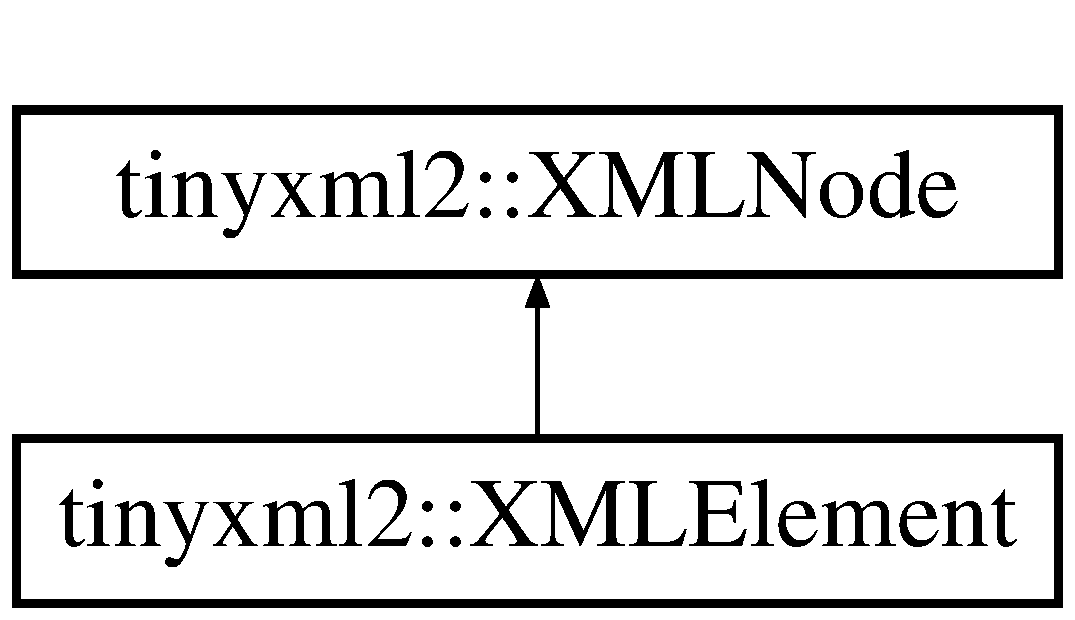
\includegraphics[height=2.000000cm]{classtinyxml2_1_1_x_m_l_element}
\end{center}
\end{figure}
\subsection*{Public Types}
\begin{DoxyCompactItemize}
\item 
enum \{ {\bfseries O\-P\-E\-N}, 
{\bfseries C\-L\-O\-S\-E\-D}, 
{\bfseries C\-L\-O\-S\-I\-N\-G}
 \}
\end{DoxyCompactItemize}
\subsection*{Public Member Functions}
\begin{DoxyCompactItemize}
\item 
\hypertarget{classtinyxml2_1_1_x_m_l_element_a8bff355472bce2c60d4b50a212bf7f5f}{const char $\ast$ \hyperlink{classtinyxml2_1_1_x_m_l_element_a8bff355472bce2c60d4b50a212bf7f5f}{Name} () const }\label{classtinyxml2_1_1_x_m_l_element_a8bff355472bce2c60d4b50a212bf7f5f}

\begin{DoxyCompactList}\small\item\em Get the name of an element (which is the \hyperlink{classtinyxml2_1_1_x_m_l_node_a7682be117e3b2b4ebfd517c1acaaadbf}{Value()} of the node.) \end{DoxyCompactList}\item 
\hypertarget{classtinyxml2_1_1_x_m_l_element_a97712009a530d8cb8a63bf705f02b4f1}{void \hyperlink{classtinyxml2_1_1_x_m_l_element_a97712009a530d8cb8a63bf705f02b4f1}{Set\-Name} (const char $\ast$str, bool static\-Mem=false)}\label{classtinyxml2_1_1_x_m_l_element_a97712009a530d8cb8a63bf705f02b4f1}

\begin{DoxyCompactList}\small\item\em Set the name of the element. \end{DoxyCompactList}\item 
\hypertarget{classtinyxml2_1_1_x_m_l_element_ad9ff5c2dbc15df36cf664ce1b0ea0a5d}{virtual \hyperlink{classtinyxml2_1_1_x_m_l_element}{X\-M\-L\-Element} $\ast$ \hyperlink{classtinyxml2_1_1_x_m_l_element_ad9ff5c2dbc15df36cf664ce1b0ea0a5d}{To\-Element} ()}\label{classtinyxml2_1_1_x_m_l_element_ad9ff5c2dbc15df36cf664ce1b0ea0a5d}

\begin{DoxyCompactList}\small\item\em Safely cast to an Element, or null. \end{DoxyCompactList}\item 
\hypertarget{classtinyxml2_1_1_x_m_l_element_a55acab615353ddabab48271f95816b0d}{virtual const \hyperlink{classtinyxml2_1_1_x_m_l_element}{X\-M\-L\-Element} $\ast$ {\bfseries To\-Element} () const }\label{classtinyxml2_1_1_x_m_l_element_a55acab615353ddabab48271f95816b0d}

\item 
virtual bool \hyperlink{classtinyxml2_1_1_x_m_l_element_a36d65438991a1e85096caf39ad13a099}{Accept} (\hyperlink{classtinyxml2_1_1_x_m_l_visitor}{X\-M\-L\-Visitor} $\ast$visitor) const 
\item 
const char $\ast$ \hyperlink{classtinyxml2_1_1_x_m_l_element_a7bdebdf1888074087237f3dd03912740}{Attribute} (const char $\ast$name, const char $\ast$value=0) const 
\item 
int \hyperlink{classtinyxml2_1_1_x_m_l_element_af86f05771c11a73a2896b662bb589ef5}{Int\-Attribute} (const char $\ast$name) const 
\item 
\hypertarget{classtinyxml2_1_1_x_m_l_element_aa5a41367b5118acec42a87f5f94cec2d}{unsigned \hyperlink{classtinyxml2_1_1_x_m_l_element_aa5a41367b5118acec42a87f5f94cec2d}{Unsigned\-Attribute} (const char $\ast$name) const }\label{classtinyxml2_1_1_x_m_l_element_aa5a41367b5118acec42a87f5f94cec2d}

\begin{DoxyCompactList}\small\item\em See \hyperlink{classtinyxml2_1_1_x_m_l_element_af86f05771c11a73a2896b662bb589ef5}{Int\-Attribute()} \end{DoxyCompactList}\item 
\hypertarget{classtinyxml2_1_1_x_m_l_element_a34811e4d1881e4ecc95c49f0f3799115}{bool \hyperlink{classtinyxml2_1_1_x_m_l_element_a34811e4d1881e4ecc95c49f0f3799115}{Bool\-Attribute} (const char $\ast$name) const }\label{classtinyxml2_1_1_x_m_l_element_a34811e4d1881e4ecc95c49f0f3799115}

\begin{DoxyCompactList}\small\item\em See \hyperlink{classtinyxml2_1_1_x_m_l_element_af86f05771c11a73a2896b662bb589ef5}{Int\-Attribute()} \end{DoxyCompactList}\item 
\hypertarget{classtinyxml2_1_1_x_m_l_element_a536922a5cae9c9769a3dc1b7a8ff0d44}{double \hyperlink{classtinyxml2_1_1_x_m_l_element_a536922a5cae9c9769a3dc1b7a8ff0d44}{Double\-Attribute} (const char $\ast$name) const }\label{classtinyxml2_1_1_x_m_l_element_a536922a5cae9c9769a3dc1b7a8ff0d44}

\begin{DoxyCompactList}\small\item\em See \hyperlink{classtinyxml2_1_1_x_m_l_element_af86f05771c11a73a2896b662bb589ef5}{Int\-Attribute()} \end{DoxyCompactList}\item 
\hypertarget{classtinyxml2_1_1_x_m_l_element_a33b69f123f995aff966d2e351bc51b1f}{float \hyperlink{classtinyxml2_1_1_x_m_l_element_a33b69f123f995aff966d2e351bc51b1f}{Float\-Attribute} (const char $\ast$name) const }\label{classtinyxml2_1_1_x_m_l_element_a33b69f123f995aff966d2e351bc51b1f}

\begin{DoxyCompactList}\small\item\em See \hyperlink{classtinyxml2_1_1_x_m_l_element_af86f05771c11a73a2896b662bb589ef5}{Int\-Attribute()} \end{DoxyCompactList}\item 
X\-M\-L\-Error \hyperlink{classtinyxml2_1_1_x_m_l_element_a8b92c729346aa8ea9acd59ed3e9f2378}{Query\-Int\-Attribute} (const char $\ast$name, int $\ast$value) const 
\item 
\hypertarget{classtinyxml2_1_1_x_m_l_element_aa3d8d1b9311da8fc249b4352749aaa84}{X\-M\-L\-Error \hyperlink{classtinyxml2_1_1_x_m_l_element_aa3d8d1b9311da8fc249b4352749aaa84}{Query\-Unsigned\-Attribute} (const char $\ast$name, unsigned int $\ast$value) const }\label{classtinyxml2_1_1_x_m_l_element_aa3d8d1b9311da8fc249b4352749aaa84}

\begin{DoxyCompactList}\small\item\em See \hyperlink{classtinyxml2_1_1_x_m_l_element_a8b92c729346aa8ea9acd59ed3e9f2378}{Query\-Int\-Attribute()} \end{DoxyCompactList}\item 
\hypertarget{classtinyxml2_1_1_x_m_l_element_a2a58ee941c3cda23772c887a8f8b534e}{X\-M\-L\-Error \hyperlink{classtinyxml2_1_1_x_m_l_element_a2a58ee941c3cda23772c887a8f8b534e}{Query\-Bool\-Attribute} (const char $\ast$name, bool $\ast$value) const }\label{classtinyxml2_1_1_x_m_l_element_a2a58ee941c3cda23772c887a8f8b534e}

\begin{DoxyCompactList}\small\item\em See \hyperlink{classtinyxml2_1_1_x_m_l_element_a8b92c729346aa8ea9acd59ed3e9f2378}{Query\-Int\-Attribute()} \end{DoxyCompactList}\item 
\hypertarget{classtinyxml2_1_1_x_m_l_element_a1ffeed461d3e4020b39652cd6d3cd773}{X\-M\-L\-Error \hyperlink{classtinyxml2_1_1_x_m_l_element_a1ffeed461d3e4020b39652cd6d3cd773}{Query\-Double\-Attribute} (const char $\ast$name, double $\ast$value) const }\label{classtinyxml2_1_1_x_m_l_element_a1ffeed461d3e4020b39652cd6d3cd773}

\begin{DoxyCompactList}\small\item\em See \hyperlink{classtinyxml2_1_1_x_m_l_element_a8b92c729346aa8ea9acd59ed3e9f2378}{Query\-Int\-Attribute()} \end{DoxyCompactList}\item 
\hypertarget{classtinyxml2_1_1_x_m_l_element_a3f154e0b4b6903249ff9f758921758e5}{X\-M\-L\-Error \hyperlink{classtinyxml2_1_1_x_m_l_element_a3f154e0b4b6903249ff9f758921758e5}{Query\-Float\-Attribute} (const char $\ast$name, float $\ast$value) const }\label{classtinyxml2_1_1_x_m_l_element_a3f154e0b4b6903249ff9f758921758e5}

\begin{DoxyCompactList}\small\item\em See \hyperlink{classtinyxml2_1_1_x_m_l_element_a8b92c729346aa8ea9acd59ed3e9f2378}{Query\-Int\-Attribute()} \end{DoxyCompactList}\item 
int \hyperlink{classtinyxml2_1_1_x_m_l_element_aa471a199af9f137ef371f5db1ed1016b}{Query\-Attribute} (const char $\ast$name, int $\ast$value) const 
\item 
\hypertarget{classtinyxml2_1_1_x_m_l_element_a60d18656aa70adb257eab18913aa4330}{int {\bfseries Query\-Attribute} (const char $\ast$name, unsigned int $\ast$value) const }\label{classtinyxml2_1_1_x_m_l_element_a60d18656aa70adb257eab18913aa4330}

\item 
\hypertarget{classtinyxml2_1_1_x_m_l_element_a23fa8bac4250249c476c6bfdb6cb9b9c}{int {\bfseries Query\-Attribute} (const char $\ast$name, bool $\ast$value) const }\label{classtinyxml2_1_1_x_m_l_element_a23fa8bac4250249c476c6bfdb6cb9b9c}

\item 
\hypertarget{classtinyxml2_1_1_x_m_l_element_a64aadcbf27423410e2896baf240f63f9}{int {\bfseries Query\-Attribute} (const char $\ast$name, double $\ast$value) const }\label{classtinyxml2_1_1_x_m_l_element_a64aadcbf27423410e2896baf240f63f9}

\item 
\hypertarget{classtinyxml2_1_1_x_m_l_element_afd553774be0e7760d73003058efa8df9}{int {\bfseries Query\-Attribute} (const char $\ast$name, float $\ast$value) const }\label{classtinyxml2_1_1_x_m_l_element_afd553774be0e7760d73003058efa8df9}

\item 
\hypertarget{classtinyxml2_1_1_x_m_l_element_a11943abf2d0831548c3790dd5d9f119c}{void \hyperlink{classtinyxml2_1_1_x_m_l_element_a11943abf2d0831548c3790dd5d9f119c}{Set\-Attribute} (const char $\ast$name, const char $\ast$value)}\label{classtinyxml2_1_1_x_m_l_element_a11943abf2d0831548c3790dd5d9f119c}

\begin{DoxyCompactList}\small\item\em Sets the named attribute to value. \end{DoxyCompactList}\item 
\hypertarget{classtinyxml2_1_1_x_m_l_element_aae6568c64c7f1cc88be8461ba41a79cf}{void \hyperlink{classtinyxml2_1_1_x_m_l_element_aae6568c64c7f1cc88be8461ba41a79cf}{Set\-Attribute} (const char $\ast$name, int value)}\label{classtinyxml2_1_1_x_m_l_element_aae6568c64c7f1cc88be8461ba41a79cf}

\begin{DoxyCompactList}\small\item\em Sets the named attribute to value. \end{DoxyCompactList}\item 
\hypertarget{classtinyxml2_1_1_x_m_l_element_ae143997e90064ba82326b29a9930ea8f}{void \hyperlink{classtinyxml2_1_1_x_m_l_element_ae143997e90064ba82326b29a9930ea8f}{Set\-Attribute} (const char $\ast$name, unsigned value)}\label{classtinyxml2_1_1_x_m_l_element_ae143997e90064ba82326b29a9930ea8f}

\begin{DoxyCompactList}\small\item\em Sets the named attribute to value. \end{DoxyCompactList}\item 
\hypertarget{classtinyxml2_1_1_x_m_l_element_aa848b696e6a75e4e545c6da9893b11e1}{void \hyperlink{classtinyxml2_1_1_x_m_l_element_aa848b696e6a75e4e545c6da9893b11e1}{Set\-Attribute} (const char $\ast$name, bool value)}\label{classtinyxml2_1_1_x_m_l_element_aa848b696e6a75e4e545c6da9893b11e1}

\begin{DoxyCompactList}\small\item\em Sets the named attribute to value. \end{DoxyCompactList}\item 
\hypertarget{classtinyxml2_1_1_x_m_l_element_a233397ee81e70eb5d4b814c5f8698533}{void \hyperlink{classtinyxml2_1_1_x_m_l_element_a233397ee81e70eb5d4b814c5f8698533}{Set\-Attribute} (const char $\ast$name, double value)}\label{classtinyxml2_1_1_x_m_l_element_a233397ee81e70eb5d4b814c5f8698533}

\begin{DoxyCompactList}\small\item\em Sets the named attribute to value. \end{DoxyCompactList}\item 
void \hyperlink{classtinyxml2_1_1_x_m_l_element_aebd45aa7118964c30b32fe12e944628a}{Delete\-Attribute} (const char $\ast$name)
\item 
\hypertarget{classtinyxml2_1_1_x_m_l_element_a67593e63558ffda0386699c3e4cc0b2c}{const \hyperlink{classtinyxml2_1_1_x_m_l_attribute}{X\-M\-L\-Attribute} $\ast$ \hyperlink{classtinyxml2_1_1_x_m_l_element_a67593e63558ffda0386699c3e4cc0b2c}{First\-Attribute} () const }\label{classtinyxml2_1_1_x_m_l_element_a67593e63558ffda0386699c3e4cc0b2c}

\begin{DoxyCompactList}\small\item\em Return the first attribute in the list. \end{DoxyCompactList}\item 
\hypertarget{classtinyxml2_1_1_x_m_l_element_aaf46b0799ea419e5d070ac9a357de48f}{const \hyperlink{classtinyxml2_1_1_x_m_l_attribute}{X\-M\-L\-Attribute} $\ast$ \hyperlink{classtinyxml2_1_1_x_m_l_element_aaf46b0799ea419e5d070ac9a357de48f}{Find\-Attribute} (const char $\ast$name) const }\label{classtinyxml2_1_1_x_m_l_element_aaf46b0799ea419e5d070ac9a357de48f}

\begin{DoxyCompactList}\small\item\em Query a specific attribute in the list. \end{DoxyCompactList}\item 
const char $\ast$ \hyperlink{classtinyxml2_1_1_x_m_l_element_a56cc727044dad002b978256754d43a4b}{Get\-Text} () const 
\item 
X\-M\-L\-Error \hyperlink{classtinyxml2_1_1_x_m_l_element_a71327c9a9d8840562bd204f46d0a7189}{Query\-Int\-Text} (int $\ast$ival) const 
\item 
\hypertarget{classtinyxml2_1_1_x_m_l_element_a2192091dec0c06be8b14f4e912c01758}{X\-M\-L\-Error \hyperlink{classtinyxml2_1_1_x_m_l_element_a2192091dec0c06be8b14f4e912c01758}{Query\-Unsigned\-Text} (unsigned $\ast$uval) const }\label{classtinyxml2_1_1_x_m_l_element_a2192091dec0c06be8b14f4e912c01758}

\begin{DoxyCompactList}\small\item\em See \hyperlink{classtinyxml2_1_1_x_m_l_element_a71327c9a9d8840562bd204f46d0a7189}{Query\-Int\-Text()} \end{DoxyCompactList}\item 
\hypertarget{classtinyxml2_1_1_x_m_l_element_afeb060672fa934163fc573e692b7fe38}{X\-M\-L\-Error \hyperlink{classtinyxml2_1_1_x_m_l_element_afeb060672fa934163fc573e692b7fe38}{Query\-Bool\-Text} (bool $\ast$bval) const }\label{classtinyxml2_1_1_x_m_l_element_afeb060672fa934163fc573e692b7fe38}

\begin{DoxyCompactList}\small\item\em See \hyperlink{classtinyxml2_1_1_x_m_l_element_a71327c9a9d8840562bd204f46d0a7189}{Query\-Int\-Text()} \end{DoxyCompactList}\item 
\hypertarget{classtinyxml2_1_1_x_m_l_element_aad931c42548907dbea416f7365d78b57}{X\-M\-L\-Error \hyperlink{classtinyxml2_1_1_x_m_l_element_aad931c42548907dbea416f7365d78b57}{Query\-Double\-Text} (double $\ast$dval) const }\label{classtinyxml2_1_1_x_m_l_element_aad931c42548907dbea416f7365d78b57}

\begin{DoxyCompactList}\small\item\em See \hyperlink{classtinyxml2_1_1_x_m_l_element_a71327c9a9d8840562bd204f46d0a7189}{Query\-Int\-Text()} \end{DoxyCompactList}\item 
\hypertarget{classtinyxml2_1_1_x_m_l_element_a11fa26e1dbca88e973964c1d9b597658}{X\-M\-L\-Error \hyperlink{classtinyxml2_1_1_x_m_l_element_a11fa26e1dbca88e973964c1d9b597658}{Query\-Float\-Text} (float $\ast$fval) const }\label{classtinyxml2_1_1_x_m_l_element_a11fa26e1dbca88e973964c1d9b597658}

\begin{DoxyCompactList}\small\item\em See \hyperlink{classtinyxml2_1_1_x_m_l_element_a71327c9a9d8840562bd204f46d0a7189}{Query\-Int\-Text()} \end{DoxyCompactList}\item 
\hypertarget{classtinyxml2_1_1_x_m_l_element_a2e3d9f938307a05963d7c4b8cd55754e}{int {\bfseries Closing\-Type} () const }\label{classtinyxml2_1_1_x_m_l_element_a2e3d9f938307a05963d7c4b8cd55754e}

\item 
\hypertarget{classtinyxml2_1_1_x_m_l_element_aaafdd2a5618abe80a2c1839ad3ccd492}{char $\ast$ {\bfseries Parse\-Deep} (char $\ast$p, \hyperlink{classtinyxml2_1_1_str_pair}{Str\-Pair} $\ast$end\-Tag)}\label{classtinyxml2_1_1_x_m_l_element_aaafdd2a5618abe80a2c1839ad3ccd492}

\item 
virtual \hyperlink{classtinyxml2_1_1_x_m_l_node}{X\-M\-L\-Node} $\ast$ \hyperlink{classtinyxml2_1_1_x_m_l_element_a85d85e32c18863fff1eeed53ae1ce23d}{Shallow\-Clone} (\hyperlink{classtinyxml2_1_1_x_m_l_document}{X\-M\-L\-Document} $\ast$document) const 
\item 
virtual bool \hyperlink{classtinyxml2_1_1_x_m_l_element_a25d51a2aad92625c78441457d58c85bc}{Shallow\-Equal} (const \hyperlink{classtinyxml2_1_1_x_m_l_node}{X\-M\-L\-Node} $\ast$compare) const 
\end{DoxyCompactItemize}
\subsection*{Friends}
\begin{DoxyCompactItemize}
\item 
\hypertarget{classtinyxml2_1_1_x_m_l_element_a449202cfc89e7ae5c2f81995476f9ec1}{class {\bfseries X\-M\-L\-Base}}\label{classtinyxml2_1_1_x_m_l_element_a449202cfc89e7ae5c2f81995476f9ec1}

\item 
\hypertarget{classtinyxml2_1_1_x_m_l_element_a4eee3bda60c60a30e4e8cd4ea91c4c6e}{class {\bfseries X\-M\-L\-Document}}\label{classtinyxml2_1_1_x_m_l_element_a4eee3bda60c60a30e4e8cd4ea91c4c6e}

\end{DoxyCompactItemize}
\subsection*{Additional Inherited Members}


\subsection{Detailed Description}
The element is a container class. It has a value, the element name, and can contain other elements, text, comments, and unknowns. Elements also contain an arbitrary number of attributes. 

\subsection{Member Function Documentation}
\hypertarget{classtinyxml2_1_1_x_m_l_element_a36d65438991a1e85096caf39ad13a099}{\index{tinyxml2\-::\-X\-M\-L\-Element@{tinyxml2\-::\-X\-M\-L\-Element}!Accept@{Accept}}
\index{Accept@{Accept}!tinyxml2::XMLElement@{tinyxml2\-::\-X\-M\-L\-Element}}
\subsubsection[{Accept}]{\setlength{\rightskip}{0pt plus 5cm}bool tinyxml2\-::\-X\-M\-L\-Element\-::\-Accept (
\begin{DoxyParamCaption}
\item[{{\bf X\-M\-L\-Visitor} $\ast$}]{visitor}
\end{DoxyParamCaption}
) const\hspace{0.3cm}{\ttfamily [virtual]}}}\label{classtinyxml2_1_1_x_m_l_element_a36d65438991a1e85096caf39ad13a099}
Accept a hierarchical visit of the nodes in the Tiny\-X\-M\-L-\/2 D\-O\-M. Every node in the X\-M\-L tree will be conditionally visited and the host will be called back via the \hyperlink{classtinyxml2_1_1_x_m_l_visitor}{X\-M\-L\-Visitor} interface.

This is essentially a S\-A\-X interface for Tiny\-X\-M\-L-\/2. (Note however it doesn't re-\/parse the X\-M\-L for the callbacks, so the performance of Tiny\-X\-M\-L-\/2 is unchanged by using this interface versus any other.)

The interface has been based on ideas from\-:


\begin{DoxyItemize}
\item \href{http://www.saxproject.org/}{\tt http\-://www.\-saxproject.\-org/}
\item \href{http://c2.com/cgi/wiki?HierarchicalVisitorPattern}{\tt http\-://c2.\-com/cgi/wiki?\-Hierarchical\-Visitor\-Pattern}
\end{DoxyItemize}

Which are both good references for \char`\"{}visiting\char`\"{}.

An example of using \hyperlink{classtinyxml2_1_1_x_m_l_element_a36d65438991a1e85096caf39ad13a099}{Accept()}\-: \begin{DoxyVerb}XMLPrinter printer;
tinyxmlDoc.Accept( &printer );
const char* xmlcstr = printer.CStr();
\end{DoxyVerb}
 

Implements \hyperlink{classtinyxml2_1_1_x_m_l_node_a81e66df0a44c67a7af17f3b77a152785}{tinyxml2\-::\-X\-M\-L\-Node}.

\hypertarget{classtinyxml2_1_1_x_m_l_element_a7bdebdf1888074087237f3dd03912740}{\index{tinyxml2\-::\-X\-M\-L\-Element@{tinyxml2\-::\-X\-M\-L\-Element}!Attribute@{Attribute}}
\index{Attribute@{Attribute}!tinyxml2::XMLElement@{tinyxml2\-::\-X\-M\-L\-Element}}
\subsubsection[{Attribute}]{\setlength{\rightskip}{0pt plus 5cm}const char $\ast$ tinyxml2\-::\-X\-M\-L\-Element\-::\-Attribute (
\begin{DoxyParamCaption}
\item[{const char $\ast$}]{name, }
\item[{const char $\ast$}]{value = {\ttfamily 0}}
\end{DoxyParamCaption}
) const}}\label{classtinyxml2_1_1_x_m_l_element_a7bdebdf1888074087237f3dd03912740}
Given an attribute name, \hyperlink{classtinyxml2_1_1_x_m_l_element_a7bdebdf1888074087237f3dd03912740}{Attribute()} returns the value for the attribute of that name, or null if none exists. For example\-:

\begin{DoxyVerb}const char* value = ele->Attribute( "foo" );
\end{DoxyVerb}


The 'value' parameter is normally null. However, if specified, the attribute will only be returned if the 'name' and 'value' match. This allow you to write code\-:

\begin{DoxyVerb}if ( ele->Attribute( "foo", "bar" ) ) callFooIsBar();
\end{DoxyVerb}


rather than\-: \begin{DoxyVerb}if ( ele->Attribute( "foo" ) ) {
    if ( strcmp( ele->Attribute( "foo" ), "bar" ) == 0 ) callFooIsBar();
}
\end{DoxyVerb}
 \hypertarget{classtinyxml2_1_1_x_m_l_element_aebd45aa7118964c30b32fe12e944628a}{\index{tinyxml2\-::\-X\-M\-L\-Element@{tinyxml2\-::\-X\-M\-L\-Element}!Delete\-Attribute@{Delete\-Attribute}}
\index{Delete\-Attribute@{Delete\-Attribute}!tinyxml2::XMLElement@{tinyxml2\-::\-X\-M\-L\-Element}}
\subsubsection[{Delete\-Attribute}]{\setlength{\rightskip}{0pt plus 5cm}void tinyxml2\-::\-X\-M\-L\-Element\-::\-Delete\-Attribute (
\begin{DoxyParamCaption}
\item[{const char $\ast$}]{name}
\end{DoxyParamCaption}
)}}\label{classtinyxml2_1_1_x_m_l_element_aebd45aa7118964c30b32fe12e944628a}
Delete an attribute. \hypertarget{classtinyxml2_1_1_x_m_l_element_a56cc727044dad002b978256754d43a4b}{\index{tinyxml2\-::\-X\-M\-L\-Element@{tinyxml2\-::\-X\-M\-L\-Element}!Get\-Text@{Get\-Text}}
\index{Get\-Text@{Get\-Text}!tinyxml2::XMLElement@{tinyxml2\-::\-X\-M\-L\-Element}}
\subsubsection[{Get\-Text}]{\setlength{\rightskip}{0pt plus 5cm}const char $\ast$ tinyxml2\-::\-X\-M\-L\-Element\-::\-Get\-Text (
\begin{DoxyParamCaption}
{}
\end{DoxyParamCaption}
) const}}\label{classtinyxml2_1_1_x_m_l_element_a56cc727044dad002b978256754d43a4b}
Convenience function for easy access to the text inside an element. Although easy and concise, \hyperlink{classtinyxml2_1_1_x_m_l_element_a56cc727044dad002b978256754d43a4b}{Get\-Text()} is limited compared to getting the \hyperlink{classtinyxml2_1_1_x_m_l_text}{X\-M\-L\-Text} child and accessing it directly.

If the first child of 'this' is a \hyperlink{classtinyxml2_1_1_x_m_l_text}{X\-M\-L\-Text}, the \hyperlink{classtinyxml2_1_1_x_m_l_element_a56cc727044dad002b978256754d43a4b}{Get\-Text()} returns the character string of the Text node, else null is returned.

This is a convenient method for getting the text of simple contained text\-: \begin{DoxyVerb}<foo>This is text</foo>
    const char* str = fooElement->GetText();
\end{DoxyVerb}


'str' will be a pointer to \char`\"{}\-This is text\char`\"{}.

Note that this function can be misleading. If the element foo was created from this X\-M\-L\-: \begin{DoxyVerb}    <foo><b>This is text</b></foo>
\end{DoxyVerb}


then the value of str would be null. The first child node isn't a text node, it is another element. From this X\-M\-L\-: \begin{DoxyVerb}    <foo>This is <b>text</b></foo>
\end{DoxyVerb}
 \hyperlink{classtinyxml2_1_1_x_m_l_element_a56cc727044dad002b978256754d43a4b}{Get\-Text()} will return \char`\"{}\-This is \char`\"{}. \hypertarget{classtinyxml2_1_1_x_m_l_element_af86f05771c11a73a2896b662bb589ef5}{\index{tinyxml2\-::\-X\-M\-L\-Element@{tinyxml2\-::\-X\-M\-L\-Element}!Int\-Attribute@{Int\-Attribute}}
\index{Int\-Attribute@{Int\-Attribute}!tinyxml2::XMLElement@{tinyxml2\-::\-X\-M\-L\-Element}}
\subsubsection[{Int\-Attribute}]{\setlength{\rightskip}{0pt plus 5cm}int tinyxml2\-::\-X\-M\-L\-Element\-::\-Int\-Attribute (
\begin{DoxyParamCaption}
\item[{const char $\ast$}]{name}
\end{DoxyParamCaption}
) const\hspace{0.3cm}{\ttfamily [inline]}}}\label{classtinyxml2_1_1_x_m_l_element_af86f05771c11a73a2896b662bb589ef5}
Given an attribute name, \hyperlink{classtinyxml2_1_1_x_m_l_element_af86f05771c11a73a2896b662bb589ef5}{Int\-Attribute()} returns the value of the attribute interpreted as an integer. 0 will be returned if there is an error. For a method with error checking, see \hyperlink{classtinyxml2_1_1_x_m_l_element_a8b92c729346aa8ea9acd59ed3e9f2378}{Query\-Int\-Attribute()} \hypertarget{classtinyxml2_1_1_x_m_l_element_aa471a199af9f137ef371f5db1ed1016b}{\index{tinyxml2\-::\-X\-M\-L\-Element@{tinyxml2\-::\-X\-M\-L\-Element}!Query\-Attribute@{Query\-Attribute}}
\index{Query\-Attribute@{Query\-Attribute}!tinyxml2::XMLElement@{tinyxml2\-::\-X\-M\-L\-Element}}
\subsubsection[{Query\-Attribute}]{\setlength{\rightskip}{0pt plus 5cm}int tinyxml2\-::\-X\-M\-L\-Element\-::\-Query\-Attribute (
\begin{DoxyParamCaption}
\item[{const char $\ast$}]{name, }
\item[{int $\ast$}]{value}
\end{DoxyParamCaption}
) const\hspace{0.3cm}{\ttfamily [inline]}}}\label{classtinyxml2_1_1_x_m_l_element_aa471a199af9f137ef371f5db1ed1016b}
Given an attribute name, \hyperlink{classtinyxml2_1_1_x_m_l_element_aa471a199af9f137ef371f5db1ed1016b}{Query\-Attribute()} returns X\-M\-L\-\_\-\-N\-O\-\_\-\-E\-R\-R\-O\-R, X\-M\-L\-\_\-\-W\-R\-O\-N\-G\-\_\-\-A\-T\-T\-R\-I\-B\-U\-T\-E\-\_\-\-T\-Y\-P\-E if the conversion can't be performed, or X\-M\-L\-\_\-\-N\-O\-\_\-\-A\-T\-T\-R\-I\-B\-U\-T\-E if the attribute doesn't exist. It is overloaded for the primitive types, and is a generally more convenient replacement of \hyperlink{classtinyxml2_1_1_x_m_l_element_a8b92c729346aa8ea9acd59ed3e9f2378}{Query\-Int\-Attribute()} and related functions.

If successful, the result of the conversion will be written to 'value'. If not successful, nothing will be written to 'value'. This allows you to provide default value\-:

\begin{DoxyVerb}int value = 10;
QueryAttribute( "foo", &value );        // if "foo" isn't found, value will still be 10
\end{DoxyVerb}
 \hypertarget{classtinyxml2_1_1_x_m_l_element_a8b92c729346aa8ea9acd59ed3e9f2378}{\index{tinyxml2\-::\-X\-M\-L\-Element@{tinyxml2\-::\-X\-M\-L\-Element}!Query\-Int\-Attribute@{Query\-Int\-Attribute}}
\index{Query\-Int\-Attribute@{Query\-Int\-Attribute}!tinyxml2::XMLElement@{tinyxml2\-::\-X\-M\-L\-Element}}
\subsubsection[{Query\-Int\-Attribute}]{\setlength{\rightskip}{0pt plus 5cm}X\-M\-L\-Error tinyxml2\-::\-X\-M\-L\-Element\-::\-Query\-Int\-Attribute (
\begin{DoxyParamCaption}
\item[{const char $\ast$}]{name, }
\item[{int $\ast$}]{value}
\end{DoxyParamCaption}
) const\hspace{0.3cm}{\ttfamily [inline]}}}\label{classtinyxml2_1_1_x_m_l_element_a8b92c729346aa8ea9acd59ed3e9f2378}
Given an attribute name, \hyperlink{classtinyxml2_1_1_x_m_l_element_a8b92c729346aa8ea9acd59ed3e9f2378}{Query\-Int\-Attribute()} returns X\-M\-L\-\_\-\-N\-O\-\_\-\-E\-R\-R\-O\-R, X\-M\-L\-\_\-\-W\-R\-O\-N\-G\-\_\-\-A\-T\-T\-R\-I\-B\-U\-T\-E\-\_\-\-T\-Y\-P\-E if the conversion can't be performed, or X\-M\-L\-\_\-\-N\-O\-\_\-\-A\-T\-T\-R\-I\-B\-U\-T\-E if the attribute doesn't exist. If successful, the result of the conversion will be written to 'value'. If not successful, nothing will be written to 'value'. This allows you to provide default value\-:

\begin{DoxyVerb}int value = 10;
QueryIntAttribute( "foo", &value );     // if "foo" isn't found, value will still be 10
\end{DoxyVerb}
 \hypertarget{classtinyxml2_1_1_x_m_l_element_a71327c9a9d8840562bd204f46d0a7189}{\index{tinyxml2\-::\-X\-M\-L\-Element@{tinyxml2\-::\-X\-M\-L\-Element}!Query\-Int\-Text@{Query\-Int\-Text}}
\index{Query\-Int\-Text@{Query\-Int\-Text}!tinyxml2::XMLElement@{tinyxml2\-::\-X\-M\-L\-Element}}
\subsubsection[{Query\-Int\-Text}]{\setlength{\rightskip}{0pt plus 5cm}X\-M\-L\-Error tinyxml2\-::\-X\-M\-L\-Element\-::\-Query\-Int\-Text (
\begin{DoxyParamCaption}
\item[{int $\ast$}]{ival}
\end{DoxyParamCaption}
) const}}\label{classtinyxml2_1_1_x_m_l_element_a71327c9a9d8840562bd204f46d0a7189}
Convenience method to query the value of a child text node. This is probably best shown by example. Given you have a document is this form\-: \begin{DoxyVerb}    <point>
        <x>1</x>
        <y>1.4</y>
    </point>
\end{DoxyVerb}


The \hyperlink{classtinyxml2_1_1_x_m_l_element_a71327c9a9d8840562bd204f46d0a7189}{Query\-Int\-Text()} and similar functions provide a safe and easier way to get to the \char`\"{}value\char`\"{} of x and y.

\begin{DoxyVerb}    int x = 0;
    float y = 0;    // types of x and y are contrived for example
    const XMLElement* xElement = pointElement->FirstChildElement( "x" );
    const XMLElement* yElement = pointElement->FirstChildElement( "y" );
    xElement->QueryIntText( &x );
    yElement->QueryFloatText( &y );
\end{DoxyVerb}


\begin{DoxyReturn}{Returns}
X\-M\-L\-\_\-\-S\-U\-C\-C\-E\-S\-S (0) on success, X\-M\-L\-\_\-\-C\-A\-N\-\_\-\-N\-O\-T\-\_\-\-C\-O\-N\-V\-E\-R\-T\-\_\-\-T\-E\-X\-T if the text cannot be converted to the requested type, and X\-M\-L\-\_\-\-N\-O\-\_\-\-T\-E\-X\-T\-\_\-\-N\-O\-D\-E if there is no child text to query. 
\end{DoxyReturn}
\hypertarget{classtinyxml2_1_1_x_m_l_element_a85d85e32c18863fff1eeed53ae1ce23d}{\index{tinyxml2\-::\-X\-M\-L\-Element@{tinyxml2\-::\-X\-M\-L\-Element}!Shallow\-Clone@{Shallow\-Clone}}
\index{Shallow\-Clone@{Shallow\-Clone}!tinyxml2::XMLElement@{tinyxml2\-::\-X\-M\-L\-Element}}
\subsubsection[{Shallow\-Clone}]{\setlength{\rightskip}{0pt plus 5cm}{\bf X\-M\-L\-Node} $\ast$ tinyxml2\-::\-X\-M\-L\-Element\-::\-Shallow\-Clone (
\begin{DoxyParamCaption}
\item[{{\bf X\-M\-L\-Document} $\ast$}]{document}
\end{DoxyParamCaption}
) const\hspace{0.3cm}{\ttfamily [virtual]}}}\label{classtinyxml2_1_1_x_m_l_element_a85d85e32c18863fff1eeed53ae1ce23d}
Make a copy of this node, but not its children. You may pass in a Document pointer that will be the owner of the new Node. If the 'document' is null, then the node returned will be allocated from the current Document. (this-\/$>$\hyperlink{classtinyxml2_1_1_x_m_l_node_af343d1ef0b45c0020e62d784d7e67a68}{Get\-Document()})

Note\-: if called on a \hyperlink{classtinyxml2_1_1_x_m_l_document}{X\-M\-L\-Document}, this will return null. 

Implements \hyperlink{classtinyxml2_1_1_x_m_l_node_a8402cbd3129d20e9e6024bbcc0531283}{tinyxml2\-::\-X\-M\-L\-Node}.

\hypertarget{classtinyxml2_1_1_x_m_l_element_a25d51a2aad92625c78441457d58c85bc}{\index{tinyxml2\-::\-X\-M\-L\-Element@{tinyxml2\-::\-X\-M\-L\-Element}!Shallow\-Equal@{Shallow\-Equal}}
\index{Shallow\-Equal@{Shallow\-Equal}!tinyxml2::XMLElement@{tinyxml2\-::\-X\-M\-L\-Element}}
\subsubsection[{Shallow\-Equal}]{\setlength{\rightskip}{0pt plus 5cm}bool tinyxml2\-::\-X\-M\-L\-Element\-::\-Shallow\-Equal (
\begin{DoxyParamCaption}
\item[{const {\bf X\-M\-L\-Node} $\ast$}]{compare}
\end{DoxyParamCaption}
) const\hspace{0.3cm}{\ttfamily [virtual]}}}\label{classtinyxml2_1_1_x_m_l_element_a25d51a2aad92625c78441457d58c85bc}
Test if 2 nodes are the same, but don't test children. The 2 nodes do not need to be in the same Document.

Note\-: if called on a \hyperlink{classtinyxml2_1_1_x_m_l_document}{X\-M\-L\-Document}, this will return false. 

Implements \hyperlink{classtinyxml2_1_1_x_m_l_node_a7ce18b751c3ea09eac292dca264f9226}{tinyxml2\-::\-X\-M\-L\-Node}.



The documentation for this class was generated from the following files\-:\begin{DoxyCompactItemize}
\item 
Joes\-\_\-\-S\-D\-L\-\_\-\-Framework/tinyxml2.\-h\item 
Joes\-\_\-\-S\-D\-L\-\_\-\-Framework/tinyxml2.\-cpp\end{DoxyCompactItemize}

\hypertarget{classtinyxml2_1_1_x_m_l_handle}{\section{tinyxml2\-:\-:X\-M\-L\-Handle Class Reference}
\label{classtinyxml2_1_1_x_m_l_handle}\index{tinyxml2\-::\-X\-M\-L\-Handle@{tinyxml2\-::\-X\-M\-L\-Handle}}
}


{\ttfamily \#include $<$tinyxml2.\-h$>$}

\subsection*{Public Member Functions}
\begin{DoxyCompactItemize}
\item 
\hyperlink{classtinyxml2_1_1_x_m_l_handle_a9c240a35c18f053509b4b97ddccd9793}{X\-M\-L\-Handle} (\hyperlink{classtinyxml2_1_1_x_m_l_node}{X\-M\-L\-Node} $\ast$node)
\begin{DoxyCompactList}\small\item\em Create a handle from any node (at any depth of the tree.) This can be a null pointer. \end{DoxyCompactList}\item 
\hyperlink{classtinyxml2_1_1_x_m_l_handle_aa2edbc1c0d3e3e8259bd98de7f1cf500}{X\-M\-L\-Handle} (\hyperlink{classtinyxml2_1_1_x_m_l_node}{X\-M\-L\-Node} \&node)
\begin{DoxyCompactList}\small\item\em Create a handle from a node. \end{DoxyCompactList}\item 
\hyperlink{classtinyxml2_1_1_x_m_l_handle_afd8e01e6018c07347b8e6d80272466aa}{X\-M\-L\-Handle} (const \hyperlink{classtinyxml2_1_1_x_m_l_handle}{X\-M\-L\-Handle} \&ref)
\begin{DoxyCompactList}\small\item\em Copy constructor. \end{DoxyCompactList}\item 
\hyperlink{classtinyxml2_1_1_x_m_l_handle}{X\-M\-L\-Handle} \& \hyperlink{classtinyxml2_1_1_x_m_l_handle_a75b908322bb4b83be3281b6845252b20}{operator=} (const \hyperlink{classtinyxml2_1_1_x_m_l_handle}{X\-M\-L\-Handle} \&ref)
\begin{DoxyCompactList}\small\item\em Assignment. \end{DoxyCompactList}\item 
\hyperlink{classtinyxml2_1_1_x_m_l_handle}{X\-M\-L\-Handle} \hyperlink{classtinyxml2_1_1_x_m_l_handle_a536447dc7f54c0cd11e031dad94795ae}{First\-Child} ()
\begin{DoxyCompactList}\small\item\em Get the first child of this handle. \end{DoxyCompactList}\item 
\hyperlink{classtinyxml2_1_1_x_m_l_handle}{X\-M\-L\-Handle} \hyperlink{classtinyxml2_1_1_x_m_l_handle_a99edff695a3cd3feff8a329189140a33}{First\-Child\-Element} (const char $\ast$value=0)
\begin{DoxyCompactList}\small\item\em Get the first child element of this handle. \end{DoxyCompactList}\item 
\hyperlink{classtinyxml2_1_1_x_m_l_handle}{X\-M\-L\-Handle} \hyperlink{classtinyxml2_1_1_x_m_l_handle_a9d09f04435f0f2f7d0816b0198d0517b}{Last\-Child} ()
\begin{DoxyCompactList}\small\item\em Get the last child of this handle. \end{DoxyCompactList}\item 
\hyperlink{classtinyxml2_1_1_x_m_l_handle}{X\-M\-L\-Handle} \hyperlink{classtinyxml2_1_1_x_m_l_handle_a4073e768ebc434b2605343b709a9a554}{Last\-Child\-Element} (const char $\ast$\-\_\-value=0)
\begin{DoxyCompactList}\small\item\em Get the last child element of this handle. \end{DoxyCompactList}\item 
\hyperlink{classtinyxml2_1_1_x_m_l_handle}{X\-M\-L\-Handle} \hyperlink{classtinyxml2_1_1_x_m_l_handle_a428374e756f4db4cbc287fec64eae02c}{Previous\-Sibling} ()
\begin{DoxyCompactList}\small\item\em Get the previous sibling of this handle. \end{DoxyCompactList}\item 
\hyperlink{classtinyxml2_1_1_x_m_l_handle}{X\-M\-L\-Handle} \hyperlink{classtinyxml2_1_1_x_m_l_handle_a31a0d5d060292bec5df2b2efe2eca228}{Previous\-Sibling\-Element} (const char $\ast$\-\_\-value=0)
\begin{DoxyCompactList}\small\item\em Get the previous sibling element of this handle. \end{DoxyCompactList}\item 
\hyperlink{classtinyxml2_1_1_x_m_l_handle}{X\-M\-L\-Handle} \hyperlink{classtinyxml2_1_1_x_m_l_handle_aad2eccc7c7c7b18145877c978c3850b5}{Next\-Sibling} ()
\begin{DoxyCompactList}\small\item\em Get the next sibling of this handle. \end{DoxyCompactList}\item 
\hyperlink{classtinyxml2_1_1_x_m_l_handle}{X\-M\-L\-Handle} \hyperlink{classtinyxml2_1_1_x_m_l_handle_a447c9b284cfcd5518f9e320ba14b9c46}{Next\-Sibling\-Element} (const char $\ast$\-\_\-value=0)
\begin{DoxyCompactList}\small\item\em Get the next sibling element of this handle. \end{DoxyCompactList}\item 
\hyperlink{classtinyxml2_1_1_x_m_l_node}{X\-M\-L\-Node} $\ast$ \hyperlink{classtinyxml2_1_1_x_m_l_handle_a03ea6ec970a021b71bf1219a0f6717df}{To\-Node} ()
\begin{DoxyCompactList}\small\item\em Safe cast to \hyperlink{classtinyxml2_1_1_x_m_l_node}{X\-M\-L\-Node}. This can return null. \end{DoxyCompactList}\item 
\hyperlink{classtinyxml2_1_1_x_m_l_element}{X\-M\-L\-Element} $\ast$ \hyperlink{classtinyxml2_1_1_x_m_l_handle_a5e73ed8f3f6f9619d5a8bb1862c47d99}{To\-Element} ()
\begin{DoxyCompactList}\small\item\em Safe cast to \hyperlink{classtinyxml2_1_1_x_m_l_element}{X\-M\-L\-Element}. This can return null. \end{DoxyCompactList}\item 
\hyperlink{classtinyxml2_1_1_x_m_l_text}{X\-M\-L\-Text} $\ast$ \hyperlink{classtinyxml2_1_1_x_m_l_handle_a6ab9e8cbfb41417246e5657e3842c62a}{To\-Text} ()
\begin{DoxyCompactList}\small\item\em Safe cast to \hyperlink{classtinyxml2_1_1_x_m_l_text}{X\-M\-L\-Text}. This can return null. \end{DoxyCompactList}\item 
\hyperlink{classtinyxml2_1_1_x_m_l_unknown}{X\-M\-L\-Unknown} $\ast$ \hyperlink{classtinyxml2_1_1_x_m_l_handle_aa387368a1ad8d843a9f12df863d298de}{To\-Unknown} ()
\begin{DoxyCompactList}\small\item\em Safe cast to \hyperlink{classtinyxml2_1_1_x_m_l_unknown}{X\-M\-L\-Unknown}. This can return null. \end{DoxyCompactList}\item 
\hyperlink{classtinyxml2_1_1_x_m_l_declaration}{X\-M\-L\-Declaration} $\ast$ \hyperlink{classtinyxml2_1_1_x_m_l_handle_a108858be7ee3eb53f73b5194c1aa8ff0}{To\-Declaration} ()
\begin{DoxyCompactList}\small\item\em Safe cast to \hyperlink{classtinyxml2_1_1_x_m_l_declaration}{X\-M\-L\-Declaration}. This can return null. \end{DoxyCompactList}\end{DoxyCompactItemize}


\subsection{Detailed Description}
A \hyperlink{classtinyxml2_1_1_x_m_l_handle}{X\-M\-L\-Handle} is a class that wraps a node pointer with null checks; this is an incredibly useful thing. Note that \hyperlink{classtinyxml2_1_1_x_m_l_handle}{X\-M\-L\-Handle} is not part of the Tiny\-X\-M\-L-\/2 D\-O\-M structure. It is a separate utility class.

Take an example\-: \begin{DoxyVerb}<Document>
    <Element attributeA = "valueA">
        <Child attributeB = "value1" />
        <Child attributeB = "value2" />
    </Element>
</Document>
\end{DoxyVerb}


Assuming you want the value of \char`\"{}attribute\-B\char`\"{} in the 2nd \char`\"{}\-Child\char`\"{} element, it's very easy to write a {\itshape lot} of code that looks like\-:

\begin{DoxyVerb}XMLElement* root = document.FirstChildElement( "Document" );
if ( root )
{
    XMLElement* element = root->FirstChildElement( "Element" );
    if ( element )
    {
        XMLElement* child = element->FirstChildElement( "Child" );
        if ( child )
        {
            XMLElement* child2 = child->NextSiblingElement( "Child" );
            if ( child2 )
            {
                // Finally do something useful.
\end{DoxyVerb}


And that doesn't even cover \char`\"{}else\char`\"{} cases. \hyperlink{classtinyxml2_1_1_x_m_l_handle}{X\-M\-L\-Handle} addresses the verbosity of such code. A \hyperlink{classtinyxml2_1_1_x_m_l_handle}{X\-M\-L\-Handle} checks for null pointers so it is perfectly safe and correct to use\-:

\begin{DoxyVerb}XMLHandle docHandle( &document );
XMLElement* child2 = docHandle.FirstChild( "Document" ).FirstChild( "Element" ).FirstChild().NextSibling().ToElement();
if ( child2 )
{
    // do something useful
\end{DoxyVerb}


Which is M\-U\-C\-H more concise and useful.

It is also safe to copy handles -\/ internally they are nothing more than node pointers. \begin{DoxyVerb}XMLHandle handleCopy = handle;
\end{DoxyVerb}


See also \hyperlink{classtinyxml2_1_1_x_m_l_const_handle}{X\-M\-L\-Const\-Handle}, which is the same as \hyperlink{classtinyxml2_1_1_x_m_l_handle}{X\-M\-L\-Handle}, but operates on const objects. 

\subsection{Constructor \& Destructor Documentation}
\hypertarget{classtinyxml2_1_1_x_m_l_handle_a9c240a35c18f053509b4b97ddccd9793}{\index{tinyxml2\-::\-X\-M\-L\-Handle@{tinyxml2\-::\-X\-M\-L\-Handle}!X\-M\-L\-Handle@{X\-M\-L\-Handle}}
\index{X\-M\-L\-Handle@{X\-M\-L\-Handle}!tinyxml2::XMLHandle@{tinyxml2\-::\-X\-M\-L\-Handle}}
\subsubsection[{X\-M\-L\-Handle}]{\setlength{\rightskip}{0pt plus 5cm}tinyxml2\-::\-X\-M\-L\-Handle\-::\-X\-M\-L\-Handle (
\begin{DoxyParamCaption}
\item[{{\bf X\-M\-L\-Node} $\ast$}]{node}
\end{DoxyParamCaption}
)\hspace{0.3cm}{\ttfamily [inline]}}}\label{classtinyxml2_1_1_x_m_l_handle_a9c240a35c18f053509b4b97ddccd9793}


Create a handle from any node (at any depth of the tree.) This can be a null pointer. 

\hypertarget{classtinyxml2_1_1_x_m_l_handle_aa2edbc1c0d3e3e8259bd98de7f1cf500}{\index{tinyxml2\-::\-X\-M\-L\-Handle@{tinyxml2\-::\-X\-M\-L\-Handle}!X\-M\-L\-Handle@{X\-M\-L\-Handle}}
\index{X\-M\-L\-Handle@{X\-M\-L\-Handle}!tinyxml2::XMLHandle@{tinyxml2\-::\-X\-M\-L\-Handle}}
\subsubsection[{X\-M\-L\-Handle}]{\setlength{\rightskip}{0pt plus 5cm}tinyxml2\-::\-X\-M\-L\-Handle\-::\-X\-M\-L\-Handle (
\begin{DoxyParamCaption}
\item[{{\bf X\-M\-L\-Node} \&}]{node}
\end{DoxyParamCaption}
)\hspace{0.3cm}{\ttfamily [inline]}}}\label{classtinyxml2_1_1_x_m_l_handle_aa2edbc1c0d3e3e8259bd98de7f1cf500}


Create a handle from a node. 

\hypertarget{classtinyxml2_1_1_x_m_l_handle_afd8e01e6018c07347b8e6d80272466aa}{\index{tinyxml2\-::\-X\-M\-L\-Handle@{tinyxml2\-::\-X\-M\-L\-Handle}!X\-M\-L\-Handle@{X\-M\-L\-Handle}}
\index{X\-M\-L\-Handle@{X\-M\-L\-Handle}!tinyxml2::XMLHandle@{tinyxml2\-::\-X\-M\-L\-Handle}}
\subsubsection[{X\-M\-L\-Handle}]{\setlength{\rightskip}{0pt plus 5cm}tinyxml2\-::\-X\-M\-L\-Handle\-::\-X\-M\-L\-Handle (
\begin{DoxyParamCaption}
\item[{const {\bf X\-M\-L\-Handle} \&}]{ref}
\end{DoxyParamCaption}
)\hspace{0.3cm}{\ttfamily [inline]}}}\label{classtinyxml2_1_1_x_m_l_handle_afd8e01e6018c07347b8e6d80272466aa}


Copy constructor. 



\subsection{Member Function Documentation}
\hypertarget{classtinyxml2_1_1_x_m_l_handle_a536447dc7f54c0cd11e031dad94795ae}{\index{tinyxml2\-::\-X\-M\-L\-Handle@{tinyxml2\-::\-X\-M\-L\-Handle}!First\-Child@{First\-Child}}
\index{First\-Child@{First\-Child}!tinyxml2::XMLHandle@{tinyxml2\-::\-X\-M\-L\-Handle}}
\subsubsection[{First\-Child}]{\setlength{\rightskip}{0pt plus 5cm}{\bf X\-M\-L\-Handle} tinyxml2\-::\-X\-M\-L\-Handle\-::\-First\-Child (
\begin{DoxyParamCaption}
{}
\end{DoxyParamCaption}
)\hspace{0.3cm}{\ttfamily [inline]}}}\label{classtinyxml2_1_1_x_m_l_handle_a536447dc7f54c0cd11e031dad94795ae}


Get the first child of this handle. 

\hypertarget{classtinyxml2_1_1_x_m_l_handle_a99edff695a3cd3feff8a329189140a33}{\index{tinyxml2\-::\-X\-M\-L\-Handle@{tinyxml2\-::\-X\-M\-L\-Handle}!First\-Child\-Element@{First\-Child\-Element}}
\index{First\-Child\-Element@{First\-Child\-Element}!tinyxml2::XMLHandle@{tinyxml2\-::\-X\-M\-L\-Handle}}
\subsubsection[{First\-Child\-Element}]{\setlength{\rightskip}{0pt plus 5cm}{\bf X\-M\-L\-Handle} tinyxml2\-::\-X\-M\-L\-Handle\-::\-First\-Child\-Element (
\begin{DoxyParamCaption}
\item[{const char $\ast$}]{value = {\ttfamily 0}}
\end{DoxyParamCaption}
)\hspace{0.3cm}{\ttfamily [inline]}}}\label{classtinyxml2_1_1_x_m_l_handle_a99edff695a3cd3feff8a329189140a33}


Get the first child element of this handle. 

\hypertarget{classtinyxml2_1_1_x_m_l_handle_a9d09f04435f0f2f7d0816b0198d0517b}{\index{tinyxml2\-::\-X\-M\-L\-Handle@{tinyxml2\-::\-X\-M\-L\-Handle}!Last\-Child@{Last\-Child}}
\index{Last\-Child@{Last\-Child}!tinyxml2::XMLHandle@{tinyxml2\-::\-X\-M\-L\-Handle}}
\subsubsection[{Last\-Child}]{\setlength{\rightskip}{0pt plus 5cm}{\bf X\-M\-L\-Handle} tinyxml2\-::\-X\-M\-L\-Handle\-::\-Last\-Child (
\begin{DoxyParamCaption}
{}
\end{DoxyParamCaption}
)\hspace{0.3cm}{\ttfamily [inline]}}}\label{classtinyxml2_1_1_x_m_l_handle_a9d09f04435f0f2f7d0816b0198d0517b}


Get the last child of this handle. 

\hypertarget{classtinyxml2_1_1_x_m_l_handle_a4073e768ebc434b2605343b709a9a554}{\index{tinyxml2\-::\-X\-M\-L\-Handle@{tinyxml2\-::\-X\-M\-L\-Handle}!Last\-Child\-Element@{Last\-Child\-Element}}
\index{Last\-Child\-Element@{Last\-Child\-Element}!tinyxml2::XMLHandle@{tinyxml2\-::\-X\-M\-L\-Handle}}
\subsubsection[{Last\-Child\-Element}]{\setlength{\rightskip}{0pt plus 5cm}{\bf X\-M\-L\-Handle} tinyxml2\-::\-X\-M\-L\-Handle\-::\-Last\-Child\-Element (
\begin{DoxyParamCaption}
\item[{const char $\ast$}]{\-\_\-value = {\ttfamily 0}}
\end{DoxyParamCaption}
)\hspace{0.3cm}{\ttfamily [inline]}}}\label{classtinyxml2_1_1_x_m_l_handle_a4073e768ebc434b2605343b709a9a554}


Get the last child element of this handle. 

\hypertarget{classtinyxml2_1_1_x_m_l_handle_aad2eccc7c7c7b18145877c978c3850b5}{\index{tinyxml2\-::\-X\-M\-L\-Handle@{tinyxml2\-::\-X\-M\-L\-Handle}!Next\-Sibling@{Next\-Sibling}}
\index{Next\-Sibling@{Next\-Sibling}!tinyxml2::XMLHandle@{tinyxml2\-::\-X\-M\-L\-Handle}}
\subsubsection[{Next\-Sibling}]{\setlength{\rightskip}{0pt plus 5cm}{\bf X\-M\-L\-Handle} tinyxml2\-::\-X\-M\-L\-Handle\-::\-Next\-Sibling (
\begin{DoxyParamCaption}
{}
\end{DoxyParamCaption}
)\hspace{0.3cm}{\ttfamily [inline]}}}\label{classtinyxml2_1_1_x_m_l_handle_aad2eccc7c7c7b18145877c978c3850b5}


Get the next sibling of this handle. 

\hypertarget{classtinyxml2_1_1_x_m_l_handle_a447c9b284cfcd5518f9e320ba14b9c46}{\index{tinyxml2\-::\-X\-M\-L\-Handle@{tinyxml2\-::\-X\-M\-L\-Handle}!Next\-Sibling\-Element@{Next\-Sibling\-Element}}
\index{Next\-Sibling\-Element@{Next\-Sibling\-Element}!tinyxml2::XMLHandle@{tinyxml2\-::\-X\-M\-L\-Handle}}
\subsubsection[{Next\-Sibling\-Element}]{\setlength{\rightskip}{0pt plus 5cm}{\bf X\-M\-L\-Handle} tinyxml2\-::\-X\-M\-L\-Handle\-::\-Next\-Sibling\-Element (
\begin{DoxyParamCaption}
\item[{const char $\ast$}]{\-\_\-value = {\ttfamily 0}}
\end{DoxyParamCaption}
)\hspace{0.3cm}{\ttfamily [inline]}}}\label{classtinyxml2_1_1_x_m_l_handle_a447c9b284cfcd5518f9e320ba14b9c46}


Get the next sibling element of this handle. 

\hypertarget{classtinyxml2_1_1_x_m_l_handle_a75b908322bb4b83be3281b6845252b20}{\index{tinyxml2\-::\-X\-M\-L\-Handle@{tinyxml2\-::\-X\-M\-L\-Handle}!operator=@{operator=}}
\index{operator=@{operator=}!tinyxml2::XMLHandle@{tinyxml2\-::\-X\-M\-L\-Handle}}
\subsubsection[{operator=}]{\setlength{\rightskip}{0pt plus 5cm}{\bf X\-M\-L\-Handle}\& tinyxml2\-::\-X\-M\-L\-Handle\-::operator= (
\begin{DoxyParamCaption}
\item[{const {\bf X\-M\-L\-Handle} \&}]{ref}
\end{DoxyParamCaption}
)\hspace{0.3cm}{\ttfamily [inline]}}}\label{classtinyxml2_1_1_x_m_l_handle_a75b908322bb4b83be3281b6845252b20}


Assignment. 

\hypertarget{classtinyxml2_1_1_x_m_l_handle_a428374e756f4db4cbc287fec64eae02c}{\index{tinyxml2\-::\-X\-M\-L\-Handle@{tinyxml2\-::\-X\-M\-L\-Handle}!Previous\-Sibling@{Previous\-Sibling}}
\index{Previous\-Sibling@{Previous\-Sibling}!tinyxml2::XMLHandle@{tinyxml2\-::\-X\-M\-L\-Handle}}
\subsubsection[{Previous\-Sibling}]{\setlength{\rightskip}{0pt plus 5cm}{\bf X\-M\-L\-Handle} tinyxml2\-::\-X\-M\-L\-Handle\-::\-Previous\-Sibling (
\begin{DoxyParamCaption}
{}
\end{DoxyParamCaption}
)\hspace{0.3cm}{\ttfamily [inline]}}}\label{classtinyxml2_1_1_x_m_l_handle_a428374e756f4db4cbc287fec64eae02c}


Get the previous sibling of this handle. 

\hypertarget{classtinyxml2_1_1_x_m_l_handle_a31a0d5d060292bec5df2b2efe2eca228}{\index{tinyxml2\-::\-X\-M\-L\-Handle@{tinyxml2\-::\-X\-M\-L\-Handle}!Previous\-Sibling\-Element@{Previous\-Sibling\-Element}}
\index{Previous\-Sibling\-Element@{Previous\-Sibling\-Element}!tinyxml2::XMLHandle@{tinyxml2\-::\-X\-M\-L\-Handle}}
\subsubsection[{Previous\-Sibling\-Element}]{\setlength{\rightskip}{0pt plus 5cm}{\bf X\-M\-L\-Handle} tinyxml2\-::\-X\-M\-L\-Handle\-::\-Previous\-Sibling\-Element (
\begin{DoxyParamCaption}
\item[{const char $\ast$}]{\-\_\-value = {\ttfamily 0}}
\end{DoxyParamCaption}
)\hspace{0.3cm}{\ttfamily [inline]}}}\label{classtinyxml2_1_1_x_m_l_handle_a31a0d5d060292bec5df2b2efe2eca228}


Get the previous sibling element of this handle. 

\hypertarget{classtinyxml2_1_1_x_m_l_handle_a108858be7ee3eb53f73b5194c1aa8ff0}{\index{tinyxml2\-::\-X\-M\-L\-Handle@{tinyxml2\-::\-X\-M\-L\-Handle}!To\-Declaration@{To\-Declaration}}
\index{To\-Declaration@{To\-Declaration}!tinyxml2::XMLHandle@{tinyxml2\-::\-X\-M\-L\-Handle}}
\subsubsection[{To\-Declaration}]{\setlength{\rightskip}{0pt plus 5cm}{\bf X\-M\-L\-Declaration}$\ast$ tinyxml2\-::\-X\-M\-L\-Handle\-::\-To\-Declaration (
\begin{DoxyParamCaption}
{}
\end{DoxyParamCaption}
)\hspace{0.3cm}{\ttfamily [inline]}}}\label{classtinyxml2_1_1_x_m_l_handle_a108858be7ee3eb53f73b5194c1aa8ff0}


Safe cast to \hyperlink{classtinyxml2_1_1_x_m_l_declaration}{X\-M\-L\-Declaration}. This can return null. 

\hypertarget{classtinyxml2_1_1_x_m_l_handle_a5e73ed8f3f6f9619d5a8bb1862c47d99}{\index{tinyxml2\-::\-X\-M\-L\-Handle@{tinyxml2\-::\-X\-M\-L\-Handle}!To\-Element@{To\-Element}}
\index{To\-Element@{To\-Element}!tinyxml2::XMLHandle@{tinyxml2\-::\-X\-M\-L\-Handle}}
\subsubsection[{To\-Element}]{\setlength{\rightskip}{0pt plus 5cm}{\bf X\-M\-L\-Element}$\ast$ tinyxml2\-::\-X\-M\-L\-Handle\-::\-To\-Element (
\begin{DoxyParamCaption}
{}
\end{DoxyParamCaption}
)\hspace{0.3cm}{\ttfamily [inline]}}}\label{classtinyxml2_1_1_x_m_l_handle_a5e73ed8f3f6f9619d5a8bb1862c47d99}


Safe cast to \hyperlink{classtinyxml2_1_1_x_m_l_element}{X\-M\-L\-Element}. This can return null. 

\hypertarget{classtinyxml2_1_1_x_m_l_handle_a03ea6ec970a021b71bf1219a0f6717df}{\index{tinyxml2\-::\-X\-M\-L\-Handle@{tinyxml2\-::\-X\-M\-L\-Handle}!To\-Node@{To\-Node}}
\index{To\-Node@{To\-Node}!tinyxml2::XMLHandle@{tinyxml2\-::\-X\-M\-L\-Handle}}
\subsubsection[{To\-Node}]{\setlength{\rightskip}{0pt plus 5cm}{\bf X\-M\-L\-Node}$\ast$ tinyxml2\-::\-X\-M\-L\-Handle\-::\-To\-Node (
\begin{DoxyParamCaption}
{}
\end{DoxyParamCaption}
)\hspace{0.3cm}{\ttfamily [inline]}}}\label{classtinyxml2_1_1_x_m_l_handle_a03ea6ec970a021b71bf1219a0f6717df}


Safe cast to \hyperlink{classtinyxml2_1_1_x_m_l_node}{X\-M\-L\-Node}. This can return null. 

\hypertarget{classtinyxml2_1_1_x_m_l_handle_a6ab9e8cbfb41417246e5657e3842c62a}{\index{tinyxml2\-::\-X\-M\-L\-Handle@{tinyxml2\-::\-X\-M\-L\-Handle}!To\-Text@{To\-Text}}
\index{To\-Text@{To\-Text}!tinyxml2::XMLHandle@{tinyxml2\-::\-X\-M\-L\-Handle}}
\subsubsection[{To\-Text}]{\setlength{\rightskip}{0pt plus 5cm}{\bf X\-M\-L\-Text}$\ast$ tinyxml2\-::\-X\-M\-L\-Handle\-::\-To\-Text (
\begin{DoxyParamCaption}
{}
\end{DoxyParamCaption}
)\hspace{0.3cm}{\ttfamily [inline]}}}\label{classtinyxml2_1_1_x_m_l_handle_a6ab9e8cbfb41417246e5657e3842c62a}


Safe cast to \hyperlink{classtinyxml2_1_1_x_m_l_text}{X\-M\-L\-Text}. This can return null. 

\hypertarget{classtinyxml2_1_1_x_m_l_handle_aa387368a1ad8d843a9f12df863d298de}{\index{tinyxml2\-::\-X\-M\-L\-Handle@{tinyxml2\-::\-X\-M\-L\-Handle}!To\-Unknown@{To\-Unknown}}
\index{To\-Unknown@{To\-Unknown}!tinyxml2::XMLHandle@{tinyxml2\-::\-X\-M\-L\-Handle}}
\subsubsection[{To\-Unknown}]{\setlength{\rightskip}{0pt plus 5cm}{\bf X\-M\-L\-Unknown}$\ast$ tinyxml2\-::\-X\-M\-L\-Handle\-::\-To\-Unknown (
\begin{DoxyParamCaption}
{}
\end{DoxyParamCaption}
)\hspace{0.3cm}{\ttfamily [inline]}}}\label{classtinyxml2_1_1_x_m_l_handle_aa387368a1ad8d843a9f12df863d298de}


Safe cast to \hyperlink{classtinyxml2_1_1_x_m_l_unknown}{X\-M\-L\-Unknown}. This can return null. 



The documentation for this class was generated from the following file\-:\begin{DoxyCompactItemize}
\item 
Joes\-\_\-\-S\-D\-L\-\_\-\-Framework/\hyperlink{tinyxml2_8h}{tinyxml2.\-h}\end{DoxyCompactItemize}

\hypertarget{classtinyxml2_1_1_x_m_l_node}{\section{tinyxml2\-:\-:X\-M\-L\-Node Class Reference}
\label{classtinyxml2_1_1_x_m_l_node}\index{tinyxml2\-::\-X\-M\-L\-Node@{tinyxml2\-::\-X\-M\-L\-Node}}
}


{\ttfamily \#include $<$tinyxml2.\-h$>$}

Inheritance diagram for tinyxml2\-:\-:X\-M\-L\-Node\-:\begin{figure}[H]
\begin{center}
\leavevmode
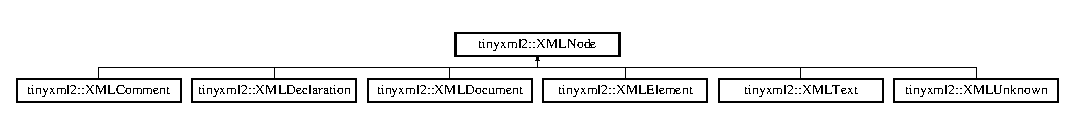
\includegraphics[height=1.145194cm]{classtinyxml2_1_1_x_m_l_node}
\end{center}
\end{figure}
\subsection*{Public Member Functions}
\begin{DoxyCompactItemize}
\item 
const \hyperlink{classtinyxml2_1_1_x_m_l_document}{X\-M\-L\-Document} $\ast$ \hyperlink{classtinyxml2_1_1_x_m_l_node_add244bca368083fa29698db8dcf147ca}{Get\-Document} () const 
\begin{DoxyCompactList}\small\item\em Get the \hyperlink{classtinyxml2_1_1_x_m_l_document}{X\-M\-L\-Document} that owns this \hyperlink{classtinyxml2_1_1_x_m_l_node}{X\-M\-L\-Node}. \end{DoxyCompactList}\item 
\hyperlink{classtinyxml2_1_1_x_m_l_document}{X\-M\-L\-Document} $\ast$ \hyperlink{classtinyxml2_1_1_x_m_l_node_af343d1ef0b45c0020e62d784d7e67a68}{Get\-Document} ()
\begin{DoxyCompactList}\small\item\em Get the \hyperlink{classtinyxml2_1_1_x_m_l_document}{X\-M\-L\-Document} that owns this \hyperlink{classtinyxml2_1_1_x_m_l_node}{X\-M\-L\-Node}. \end{DoxyCompactList}\item 
virtual \hyperlink{classtinyxml2_1_1_x_m_l_element}{X\-M\-L\-Element} $\ast$ \hyperlink{classtinyxml2_1_1_x_m_l_node_aab516e699567f75cc9ab2ef2eee501e8}{To\-Element} ()
\begin{DoxyCompactList}\small\item\em Safely cast to an Element, or null. \end{DoxyCompactList}\item 
virtual \hyperlink{classtinyxml2_1_1_x_m_l_text}{X\-M\-L\-Text} $\ast$ \hyperlink{classtinyxml2_1_1_x_m_l_node_a41c55dab9162d1eb62db2008430e376b}{To\-Text} ()
\begin{DoxyCompactList}\small\item\em Safely cast to Text, or null. \end{DoxyCompactList}\item 
virtual \hyperlink{classtinyxml2_1_1_x_m_l_comment}{X\-M\-L\-Comment} $\ast$ \hyperlink{classtinyxml2_1_1_x_m_l_node_aff47671055aa99840a1c1ebd661e63e3}{To\-Comment} ()
\begin{DoxyCompactList}\small\item\em Safely cast to a Comment, or null. \end{DoxyCompactList}\item 
virtual \hyperlink{classtinyxml2_1_1_x_m_l_document}{X\-M\-L\-Document} $\ast$ \hyperlink{classtinyxml2_1_1_x_m_l_node_a836e2966ed736fc3c94f70e12a2a3357}{To\-Document} ()
\begin{DoxyCompactList}\small\item\em Safely cast to a Document, or null. \end{DoxyCompactList}\item 
virtual \hyperlink{classtinyxml2_1_1_x_m_l_declaration}{X\-M\-L\-Declaration} $\ast$ \hyperlink{classtinyxml2_1_1_x_m_l_node_a174fd4c22c010b58138c1b84a0dfbd51}{To\-Declaration} ()
\begin{DoxyCompactList}\small\item\em Safely cast to a Declaration, or null. \end{DoxyCompactList}\item 
virtual \hyperlink{classtinyxml2_1_1_x_m_l_unknown}{X\-M\-L\-Unknown} $\ast$ \hyperlink{classtinyxml2_1_1_x_m_l_node_a8675a74aa0ada6eccab0c77ef3e5b9bd}{To\-Unknown} ()
\begin{DoxyCompactList}\small\item\em Safely cast to an Unknown, or null. \end{DoxyCompactList}\item 
virtual const \hyperlink{classtinyxml2_1_1_x_m_l_element}{X\-M\-L\-Element} $\ast$ \hyperlink{classtinyxml2_1_1_x_m_l_node_acbaec609797ddabb4f9dcf38ee91262e}{To\-Element} () const 
\item 
virtual const \hyperlink{classtinyxml2_1_1_x_m_l_text}{X\-M\-L\-Text} $\ast$ \hyperlink{classtinyxml2_1_1_x_m_l_node_a89009ffc1b9f5d692bf8d4c9f18c3bec}{To\-Text} () const 
\item 
virtual const \hyperlink{classtinyxml2_1_1_x_m_l_comment}{X\-M\-L\-Comment} $\ast$ \hyperlink{classtinyxml2_1_1_x_m_l_node_a157ce3a00ea5ee5a85b7103138e85e8a}{To\-Comment} () const 
\item 
virtual const \hyperlink{classtinyxml2_1_1_x_m_l_document}{X\-M\-L\-Document} $\ast$ \hyperlink{classtinyxml2_1_1_x_m_l_node_a3ff975733a17d6ced3539b45544c8bf6}{To\-Document} () const 
\item 
virtual const \hyperlink{classtinyxml2_1_1_x_m_l_declaration}{X\-M\-L\-Declaration} $\ast$ \hyperlink{classtinyxml2_1_1_x_m_l_node_aedae0bbb58d533a4b8a61042388b49e5}{To\-Declaration} () const 
\item 
virtual const \hyperlink{classtinyxml2_1_1_x_m_l_unknown}{X\-M\-L\-Unknown} $\ast$ \hyperlink{classtinyxml2_1_1_x_m_l_node_a71f5ae90296dbe67979f83fe97073efa}{To\-Unknown} () const 
\item 
const char $\ast$ \hyperlink{classtinyxml2_1_1_x_m_l_node_a7682be117e3b2b4ebfd517c1acaaadbf}{Value} () const 
\item 
void \hyperlink{classtinyxml2_1_1_x_m_l_node_a09dd68cf9eae137579f6e50f36487513}{Set\-Value} (const char $\ast$val, bool static\-Mem=false)
\item 
const \hyperlink{classtinyxml2_1_1_x_m_l_node}{X\-M\-L\-Node} $\ast$ \hyperlink{classtinyxml2_1_1_x_m_l_node_a4e39bdcf9bfafa55d04857ece6aaf64e}{Parent} () const 
\begin{DoxyCompactList}\small\item\em Get the parent of this node on the D\-O\-M. \end{DoxyCompactList}\item 
\hyperlink{classtinyxml2_1_1_x_m_l_node}{X\-M\-L\-Node} $\ast$ \hyperlink{classtinyxml2_1_1_x_m_l_node_a76029693a5a54fbb721a41d7a0ca8a97}{Parent} ()
\item 
bool \hyperlink{classtinyxml2_1_1_x_m_l_node_a96afe34a9ccd0ed4c0cff32beb42cc6c}{No\-Children} () const 
\begin{DoxyCompactList}\small\item\em Returns true if this node has no children. \end{DoxyCompactList}\item 
const \hyperlink{classtinyxml2_1_1_x_m_l_node}{X\-M\-L\-Node} $\ast$ \hyperlink{classtinyxml2_1_1_x_m_l_node_a60e923d13d7dc01f45ab90a2f948b02a}{First\-Child} () const 
\begin{DoxyCompactList}\small\item\em Get the first child node, or null if none exists. \end{DoxyCompactList}\item 
\hyperlink{classtinyxml2_1_1_x_m_l_node}{X\-M\-L\-Node} $\ast$ \hyperlink{classtinyxml2_1_1_x_m_l_node_a2d6c70c475146b48bc93a7fafdeff5e0}{First\-Child} ()
\item 
const \hyperlink{classtinyxml2_1_1_x_m_l_element}{X\-M\-L\-Element} $\ast$ \hyperlink{classtinyxml2_1_1_x_m_l_node_a20f48e99b03e9c17487944f229bee130}{First\-Child\-Element} (const char $\ast$value=0) const 
\item 
\hyperlink{classtinyxml2_1_1_x_m_l_element}{X\-M\-L\-Element} $\ast$ \hyperlink{classtinyxml2_1_1_x_m_l_node_a7614c3b4eea1ff11b2aa90b0f92f6dba}{First\-Child\-Element} (const char $\ast$value=0)
\item 
const \hyperlink{classtinyxml2_1_1_x_m_l_node}{X\-M\-L\-Node} $\ast$ \hyperlink{classtinyxml2_1_1_x_m_l_node_a6088246532b02895beb0e6fa561a7f3b}{Last\-Child} () const 
\begin{DoxyCompactList}\small\item\em Get the last child node, or null if none exists. \end{DoxyCompactList}\item 
\hyperlink{classtinyxml2_1_1_x_m_l_node}{X\-M\-L\-Node} $\ast$ \hyperlink{classtinyxml2_1_1_x_m_l_node_ad7552c8cb1dc0cb6f3bdc14a9d115dbf}{Last\-Child} ()
\item 
const \hyperlink{classtinyxml2_1_1_x_m_l_element}{X\-M\-L\-Element} $\ast$ \hyperlink{classtinyxml2_1_1_x_m_l_node_a1a46cc01ece2216acf1e6294d1aff79d}{Last\-Child\-Element} (const char $\ast$value=0) const 
\item 
\hyperlink{classtinyxml2_1_1_x_m_l_element}{X\-M\-L\-Element} $\ast$ \hyperlink{classtinyxml2_1_1_x_m_l_node_a125423acf3170b130634638c5afc0639}{Last\-Child\-Element} (const char $\ast$value=0)
\item 
const \hyperlink{classtinyxml2_1_1_x_m_l_node}{X\-M\-L\-Node} $\ast$ \hyperlink{classtinyxml2_1_1_x_m_l_node_a4cb1bf63e9de55129d21a7be60685fd4}{Previous\-Sibling} () const 
\begin{DoxyCompactList}\small\item\em Get the previous (left) sibling node of this node. \end{DoxyCompactList}\item 
\hyperlink{classtinyxml2_1_1_x_m_l_node}{X\-M\-L\-Node} $\ast$ \hyperlink{classtinyxml2_1_1_x_m_l_node_ae760e5e7e766df1d2cf3bb4a847876d6}{Previous\-Sibling} ()
\item 
const \hyperlink{classtinyxml2_1_1_x_m_l_element}{X\-M\-L\-Element} $\ast$ \hyperlink{classtinyxml2_1_1_x_m_l_node_a573b2559c41dce244d893d610fbe0bd9}{Previous\-Sibling\-Element} (const char $\ast$value=0) const 
\begin{DoxyCompactList}\small\item\em Get the previous (left) sibling element of this node, with an optionally supplied name. \end{DoxyCompactList}\item 
\hyperlink{classtinyxml2_1_1_x_m_l_element}{X\-M\-L\-Element} $\ast$ \hyperlink{classtinyxml2_1_1_x_m_l_node_ae9177fdc49cb89879f333581d5f734f1}{Previous\-Sibling\-Element} (const char $\ast$value=0)
\item 
const \hyperlink{classtinyxml2_1_1_x_m_l_node}{X\-M\-L\-Node} $\ast$ \hyperlink{classtinyxml2_1_1_x_m_l_node_abba1df37581d89dccc45acdc55750ba2}{Next\-Sibling} () const 
\begin{DoxyCompactList}\small\item\em Get the next (right) sibling node of this node. \end{DoxyCompactList}\item 
\hyperlink{classtinyxml2_1_1_x_m_l_node}{X\-M\-L\-Node} $\ast$ \hyperlink{classtinyxml2_1_1_x_m_l_node_aeb7d4dfd8fb924ef86e7cb72183acbac}{Next\-Sibling} ()
\item 
const \hyperlink{classtinyxml2_1_1_x_m_l_element}{X\-M\-L\-Element} $\ast$ \hyperlink{classtinyxml2_1_1_x_m_l_node_a490e166c3a1c6607960bfa9c112d3d30}{Next\-Sibling\-Element} (const char $\ast$value=0) const 
\begin{DoxyCompactList}\small\item\em Get the next (right) sibling element of this node, with an optionally supplied name. \end{DoxyCompactList}\item 
\hyperlink{classtinyxml2_1_1_x_m_l_element}{X\-M\-L\-Element} $\ast$ \hyperlink{classtinyxml2_1_1_x_m_l_node_acf735bf653016792522305d8ad4b3029}{Next\-Sibling\-Element} (const char $\ast$value=0)
\item 
\hyperlink{classtinyxml2_1_1_x_m_l_node}{X\-M\-L\-Node} $\ast$ \hyperlink{classtinyxml2_1_1_x_m_l_node_ae3b422e98914d6002ca99bb1d2837103}{Insert\-End\-Child} (\hyperlink{classtinyxml2_1_1_x_m_l_node}{X\-M\-L\-Node} $\ast$add\-This)
\item 
\hyperlink{classtinyxml2_1_1_x_m_l_node}{X\-M\-L\-Node} $\ast$ \hyperlink{classtinyxml2_1_1_x_m_l_node_a663e3a5a378169fd477378f4d17a7649}{Link\-End\-Child} (\hyperlink{classtinyxml2_1_1_x_m_l_node}{X\-M\-L\-Node} $\ast$add\-This)
\item 
\hyperlink{classtinyxml2_1_1_x_m_l_node}{X\-M\-L\-Node} $\ast$ \hyperlink{classtinyxml2_1_1_x_m_l_node_ac609a8f3ea949027f439280c640bbaf2}{Insert\-First\-Child} (\hyperlink{classtinyxml2_1_1_x_m_l_node}{X\-M\-L\-Node} $\ast$add\-This)
\item 
\hyperlink{classtinyxml2_1_1_x_m_l_node}{X\-M\-L\-Node} $\ast$ \hyperlink{classtinyxml2_1_1_x_m_l_node_a9275138a1b8dd5d8e2c26789bdc23ac8}{Insert\-After\-Child} (\hyperlink{classtinyxml2_1_1_x_m_l_node}{X\-M\-L\-Node} $\ast$after\-This, \hyperlink{classtinyxml2_1_1_x_m_l_node}{X\-M\-L\-Node} $\ast$add\-This)
\item 
void \hyperlink{classtinyxml2_1_1_x_m_l_node_a0360085cc54df5bff85d5c5da13afdce}{Delete\-Children} ()
\item 
void \hyperlink{classtinyxml2_1_1_x_m_l_node_a363b6edbd6ebd55f8387d2b89f2b0921}{Delete\-Child} (\hyperlink{classtinyxml2_1_1_x_m_l_node}{X\-M\-L\-Node} $\ast$node)
\item 
virtual \hyperlink{classtinyxml2_1_1_x_m_l_node}{X\-M\-L\-Node} $\ast$ \hyperlink{classtinyxml2_1_1_x_m_l_node_a8402cbd3129d20e9e6024bbcc0531283}{Shallow\-Clone} (\hyperlink{classtinyxml2_1_1_x_m_l_document}{X\-M\-L\-Document} $\ast$document) const =0
\item 
virtual bool \hyperlink{classtinyxml2_1_1_x_m_l_node_a7ce18b751c3ea09eac292dca264f9226}{Shallow\-Equal} (const \hyperlink{classtinyxml2_1_1_x_m_l_node}{X\-M\-L\-Node} $\ast$compare) const =0
\item 
virtual bool \hyperlink{classtinyxml2_1_1_x_m_l_node_a81e66df0a44c67a7af17f3b77a152785}{Accept} (\hyperlink{classtinyxml2_1_1_x_m_l_visitor}{X\-M\-L\-Visitor} $\ast$visitor) const =0
\item 
virtual char $\ast$ \hyperlink{classtinyxml2_1_1_x_m_l_node_a7610d0f603e8b603d2078521811a23c1}{Parse\-Deep} (char $\ast$, \hyperlink{classtinyxml2_1_1_str_pair}{Str\-Pair} $\ast$)
\end{DoxyCompactItemize}
\subsection*{Protected Member Functions}
\begin{DoxyCompactItemize}
\item 
\hyperlink{classtinyxml2_1_1_x_m_l_node_a29868df6ca383d574f584dfdd15105b6}{X\-M\-L\-Node} (\hyperlink{classtinyxml2_1_1_x_m_l_document}{X\-M\-L\-Document} $\ast$)
\item 
virtual \hyperlink{classtinyxml2_1_1_x_m_l_node_a8f41e898cdd4da4cdbb7f05b0c7d9f69}{$\sim$\-X\-M\-L\-Node} ()
\item 
\hyperlink{classtinyxml2_1_1_x_m_l_node_a78be01384518a969da905548f318d75b}{X\-M\-L\-Node} (const \hyperlink{classtinyxml2_1_1_x_m_l_node}{X\-M\-L\-Node} \&)
\item 
\hyperlink{classtinyxml2_1_1_x_m_l_node}{X\-M\-L\-Node} \& \hyperlink{classtinyxml2_1_1_x_m_l_node_ade79231d908e1f21862819e00e56ab6e}{operator=} (const \hyperlink{classtinyxml2_1_1_x_m_l_node}{X\-M\-L\-Node} \&)
\end{DoxyCompactItemize}
\subsection*{Protected Attributes}
\begin{DoxyCompactItemize}
\item 
\hyperlink{classtinyxml2_1_1_x_m_l_document}{X\-M\-L\-Document} $\ast$ \hyperlink{classtinyxml2_1_1_x_m_l_node_a8d2d2be0bb6797625551eb0e91f0ff62}{\-\_\-document}
\item 
\hyperlink{classtinyxml2_1_1_x_m_l_node}{X\-M\-L\-Node} $\ast$ \hyperlink{classtinyxml2_1_1_x_m_l_node_a176dd1c4965c21c366de192164aa2c13}{\-\_\-parent}
\item 
\hyperlink{classtinyxml2_1_1_str_pair}{Str\-Pair} \hyperlink{classtinyxml2_1_1_x_m_l_node_a3ea9884098b8379de2bb5ab3fc85c0fc}{\-\_\-value}
\item 
\hyperlink{classtinyxml2_1_1_x_m_l_node}{X\-M\-L\-Node} $\ast$ \hyperlink{classtinyxml2_1_1_x_m_l_node_aa20c91e4213dc930c5bdf420322ca342}{\-\_\-first\-Child}
\item 
\hyperlink{classtinyxml2_1_1_x_m_l_node}{X\-M\-L\-Node} $\ast$ \hyperlink{classtinyxml2_1_1_x_m_l_node_a099b6560ae44ab9edb8453aaf1a3747b}{\-\_\-last\-Child}
\item 
\hyperlink{classtinyxml2_1_1_x_m_l_node}{X\-M\-L\-Node} $\ast$ \hyperlink{classtinyxml2_1_1_x_m_l_node_a9739eb0fb9a1188266052055e7a6bf6b}{\-\_\-prev}
\item 
\hyperlink{classtinyxml2_1_1_x_m_l_node}{X\-M\-L\-Node} $\ast$ \hyperlink{classtinyxml2_1_1_x_m_l_node_a27e985496b37dd00eb5b9cf59b9e3fb1}{\-\_\-next}
\end{DoxyCompactItemize}
\subsection*{Friends}
\begin{DoxyCompactItemize}
\item 
class \hyperlink{classtinyxml2_1_1_x_m_l_node_a4eee3bda60c60a30e4e8cd4ea91c4c6e}{X\-M\-L\-Document}
\item 
class \hyperlink{classtinyxml2_1_1_x_m_l_node_ac2fba9b6e452829dd892f7392c24e0eb}{X\-M\-L\-Element}
\end{DoxyCompactItemize}


\subsection{Detailed Description}
\hyperlink{classtinyxml2_1_1_x_m_l_node}{X\-M\-L\-Node} is a base class for every object that is in the X\-M\-L Document Object Model (D\-O\-M), except X\-M\-L\-Attributes. Nodes have siblings, a parent, and children which can be navigated. A node is always in a \hyperlink{classtinyxml2_1_1_x_m_l_document}{X\-M\-L\-Document}. The type of a \hyperlink{classtinyxml2_1_1_x_m_l_node}{X\-M\-L\-Node} can be queried, and it can be cast to its more defined type.

A \hyperlink{classtinyxml2_1_1_x_m_l_document}{X\-M\-L\-Document} allocates memory for all its Nodes. When the \hyperlink{classtinyxml2_1_1_x_m_l_document}{X\-M\-L\-Document} gets deleted, all its Nodes will also be deleted.

\begin{DoxyVerb}A Document can contain: Element (container or leaf)
                        Comment (leaf)
                        Unknown (leaf)
                        Declaration( leaf )

An Element can contain: Element (container or leaf)
                        Text    (leaf)
                        Attributes (not on tree)
                        Comment (leaf)
                        Unknown (leaf)\end{DoxyVerb}
 

\subsection{Constructor \& Destructor Documentation}
\hypertarget{classtinyxml2_1_1_x_m_l_node_a29868df6ca383d574f584dfdd15105b6}{\index{tinyxml2\-::\-X\-M\-L\-Node@{tinyxml2\-::\-X\-M\-L\-Node}!X\-M\-L\-Node@{X\-M\-L\-Node}}
\index{X\-M\-L\-Node@{X\-M\-L\-Node}!tinyxml2::XMLNode@{tinyxml2\-::\-X\-M\-L\-Node}}
\subsubsection[{X\-M\-L\-Node}]{\setlength{\rightskip}{0pt plus 5cm}tinyxml2\-::\-X\-M\-L\-Node\-::\-X\-M\-L\-Node (
\begin{DoxyParamCaption}
\item[{{\bf X\-M\-L\-Document} $\ast$}]{doc}
\end{DoxyParamCaption}
)\hspace{0.3cm}{\ttfamily [protected]}}}\label{classtinyxml2_1_1_x_m_l_node_a29868df6ca383d574f584dfdd15105b6}
\hypertarget{classtinyxml2_1_1_x_m_l_node_a8f41e898cdd4da4cdbb7f05b0c7d9f69}{\index{tinyxml2\-::\-X\-M\-L\-Node@{tinyxml2\-::\-X\-M\-L\-Node}!$\sim$\-X\-M\-L\-Node@{$\sim$\-X\-M\-L\-Node}}
\index{$\sim$\-X\-M\-L\-Node@{$\sim$\-X\-M\-L\-Node}!tinyxml2::XMLNode@{tinyxml2\-::\-X\-M\-L\-Node}}
\subsubsection[{$\sim$\-X\-M\-L\-Node}]{\setlength{\rightskip}{0pt plus 5cm}tinyxml2\-::\-X\-M\-L\-Node\-::$\sim$\-X\-M\-L\-Node (
\begin{DoxyParamCaption}
{}
\end{DoxyParamCaption}
)\hspace{0.3cm}{\ttfamily [protected]}, {\ttfamily [virtual]}}}\label{classtinyxml2_1_1_x_m_l_node_a8f41e898cdd4da4cdbb7f05b0c7d9f69}
\hypertarget{classtinyxml2_1_1_x_m_l_node_a78be01384518a969da905548f318d75b}{\index{tinyxml2\-::\-X\-M\-L\-Node@{tinyxml2\-::\-X\-M\-L\-Node}!X\-M\-L\-Node@{X\-M\-L\-Node}}
\index{X\-M\-L\-Node@{X\-M\-L\-Node}!tinyxml2::XMLNode@{tinyxml2\-::\-X\-M\-L\-Node}}
\subsubsection[{X\-M\-L\-Node}]{\setlength{\rightskip}{0pt plus 5cm}tinyxml2\-::\-X\-M\-L\-Node\-::\-X\-M\-L\-Node (
\begin{DoxyParamCaption}
\item[{const {\bf X\-M\-L\-Node} \&}]{}
\end{DoxyParamCaption}
)\hspace{0.3cm}{\ttfamily [protected]}}}\label{classtinyxml2_1_1_x_m_l_node_a78be01384518a969da905548f318d75b}


\subsection{Member Function Documentation}
\hypertarget{classtinyxml2_1_1_x_m_l_node_a81e66df0a44c67a7af17f3b77a152785}{\index{tinyxml2\-::\-X\-M\-L\-Node@{tinyxml2\-::\-X\-M\-L\-Node}!Accept@{Accept}}
\index{Accept@{Accept}!tinyxml2::XMLNode@{tinyxml2\-::\-X\-M\-L\-Node}}
\subsubsection[{Accept}]{\setlength{\rightskip}{0pt plus 5cm}virtual bool tinyxml2\-::\-X\-M\-L\-Node\-::\-Accept (
\begin{DoxyParamCaption}
\item[{{\bf X\-M\-L\-Visitor} $\ast$}]{visitor}
\end{DoxyParamCaption}
) const\hspace{0.3cm}{\ttfamily [pure virtual]}}}\label{classtinyxml2_1_1_x_m_l_node_a81e66df0a44c67a7af17f3b77a152785}
Accept a hierarchical visit of the nodes in the Tiny\-X\-M\-L-\/2 D\-O\-M. Every node in the X\-M\-L tree will be conditionally visited and the host will be called back via the \hyperlink{classtinyxml2_1_1_x_m_l_visitor}{X\-M\-L\-Visitor} interface.

This is essentially a S\-A\-X interface for Tiny\-X\-M\-L-\/2. (Note however it doesn't re-\/parse the X\-M\-L for the callbacks, so the performance of Tiny\-X\-M\-L-\/2 is unchanged by using this interface versus any other.)

The interface has been based on ideas from\-:


\begin{DoxyItemize}
\item \href{http://www.saxproject.org/}{\tt http\-://www.\-saxproject.\-org/}
\item \href{http://c2.com/cgi/wiki?HierarchicalVisitorPattern}{\tt http\-://c2.\-com/cgi/wiki?\-Hierarchical\-Visitor\-Pattern}
\end{DoxyItemize}

Which are both good references for \char`\"{}visiting\char`\"{}.

An example of using \hyperlink{classtinyxml2_1_1_x_m_l_node_a81e66df0a44c67a7af17f3b77a152785}{Accept()}\-: \begin{DoxyVerb}XMLPrinter printer;
tinyxmlDoc.Accept( &printer );
const char* xmlcstr = printer.CStr();
\end{DoxyVerb}
 

Implemented in \hyperlink{classtinyxml2_1_1_x_m_l_document_aa08503d24898bf9992ae5e5fb8b0cf87}{tinyxml2\-::\-X\-M\-L\-Document}, \hyperlink{classtinyxml2_1_1_x_m_l_element_a36d65438991a1e85096caf39ad13a099}{tinyxml2\-::\-X\-M\-L\-Element}, \hyperlink{classtinyxml2_1_1_x_m_l_unknown_a0d341ab804a1438a474810bb5bd29dd5}{tinyxml2\-::\-X\-M\-L\-Unknown}, \hyperlink{classtinyxml2_1_1_x_m_l_declaration_a953a7359cc312d15218eb5843a4ca108}{tinyxml2\-::\-X\-M\-L\-Declaration}, \hyperlink{classtinyxml2_1_1_x_m_l_comment_aa382b1be6a8b0650c16a2d88bb499335}{tinyxml2\-::\-X\-M\-L\-Comment}, and \hyperlink{classtinyxml2_1_1_x_m_l_text_ae659d4fc7351a7df11c111cbe1ade46f}{tinyxml2\-::\-X\-M\-L\-Text}.

\hypertarget{classtinyxml2_1_1_x_m_l_node_a363b6edbd6ebd55f8387d2b89f2b0921}{\index{tinyxml2\-::\-X\-M\-L\-Node@{tinyxml2\-::\-X\-M\-L\-Node}!Delete\-Child@{Delete\-Child}}
\index{Delete\-Child@{Delete\-Child}!tinyxml2::XMLNode@{tinyxml2\-::\-X\-M\-L\-Node}}
\subsubsection[{Delete\-Child}]{\setlength{\rightskip}{0pt plus 5cm}void tinyxml2\-::\-X\-M\-L\-Node\-::\-Delete\-Child (
\begin{DoxyParamCaption}
\item[{{\bf X\-M\-L\-Node} $\ast$}]{node}
\end{DoxyParamCaption}
)}}\label{classtinyxml2_1_1_x_m_l_node_a363b6edbd6ebd55f8387d2b89f2b0921}
Delete a child of this node. \hypertarget{classtinyxml2_1_1_x_m_l_node_a0360085cc54df5bff85d5c5da13afdce}{\index{tinyxml2\-::\-X\-M\-L\-Node@{tinyxml2\-::\-X\-M\-L\-Node}!Delete\-Children@{Delete\-Children}}
\index{Delete\-Children@{Delete\-Children}!tinyxml2::XMLNode@{tinyxml2\-::\-X\-M\-L\-Node}}
\subsubsection[{Delete\-Children}]{\setlength{\rightskip}{0pt plus 5cm}void tinyxml2\-::\-X\-M\-L\-Node\-::\-Delete\-Children (
\begin{DoxyParamCaption}
{}
\end{DoxyParamCaption}
)}}\label{classtinyxml2_1_1_x_m_l_node_a0360085cc54df5bff85d5c5da13afdce}
Delete all the children of this node. \hypertarget{classtinyxml2_1_1_x_m_l_node_a60e923d13d7dc01f45ab90a2f948b02a}{\index{tinyxml2\-::\-X\-M\-L\-Node@{tinyxml2\-::\-X\-M\-L\-Node}!First\-Child@{First\-Child}}
\index{First\-Child@{First\-Child}!tinyxml2::XMLNode@{tinyxml2\-::\-X\-M\-L\-Node}}
\subsubsection[{First\-Child}]{\setlength{\rightskip}{0pt plus 5cm}const {\bf X\-M\-L\-Node}$\ast$ tinyxml2\-::\-X\-M\-L\-Node\-::\-First\-Child (
\begin{DoxyParamCaption}
{}
\end{DoxyParamCaption}
) const\hspace{0.3cm}{\ttfamily [inline]}}}\label{classtinyxml2_1_1_x_m_l_node_a60e923d13d7dc01f45ab90a2f948b02a}


Get the first child node, or null if none exists. 

\hypertarget{classtinyxml2_1_1_x_m_l_node_a2d6c70c475146b48bc93a7fafdeff5e0}{\index{tinyxml2\-::\-X\-M\-L\-Node@{tinyxml2\-::\-X\-M\-L\-Node}!First\-Child@{First\-Child}}
\index{First\-Child@{First\-Child}!tinyxml2::XMLNode@{tinyxml2\-::\-X\-M\-L\-Node}}
\subsubsection[{First\-Child}]{\setlength{\rightskip}{0pt plus 5cm}{\bf X\-M\-L\-Node}$\ast$ tinyxml2\-::\-X\-M\-L\-Node\-::\-First\-Child (
\begin{DoxyParamCaption}
{}
\end{DoxyParamCaption}
)\hspace{0.3cm}{\ttfamily [inline]}}}\label{classtinyxml2_1_1_x_m_l_node_a2d6c70c475146b48bc93a7fafdeff5e0}
\hypertarget{classtinyxml2_1_1_x_m_l_node_a20f48e99b03e9c17487944f229bee130}{\index{tinyxml2\-::\-X\-M\-L\-Node@{tinyxml2\-::\-X\-M\-L\-Node}!First\-Child\-Element@{First\-Child\-Element}}
\index{First\-Child\-Element@{First\-Child\-Element}!tinyxml2::XMLNode@{tinyxml2\-::\-X\-M\-L\-Node}}
\subsubsection[{First\-Child\-Element}]{\setlength{\rightskip}{0pt plus 5cm}const {\bf X\-M\-L\-Element} $\ast$ tinyxml2\-::\-X\-M\-L\-Node\-::\-First\-Child\-Element (
\begin{DoxyParamCaption}
\item[{const char $\ast$}]{value = {\ttfamily 0}}
\end{DoxyParamCaption}
) const}}\label{classtinyxml2_1_1_x_m_l_node_a20f48e99b03e9c17487944f229bee130}
Get the first child element, or optionally the first child element with the specified name. \hypertarget{classtinyxml2_1_1_x_m_l_node_a7614c3b4eea1ff11b2aa90b0f92f6dba}{\index{tinyxml2\-::\-X\-M\-L\-Node@{tinyxml2\-::\-X\-M\-L\-Node}!First\-Child\-Element@{First\-Child\-Element}}
\index{First\-Child\-Element@{First\-Child\-Element}!tinyxml2::XMLNode@{tinyxml2\-::\-X\-M\-L\-Node}}
\subsubsection[{First\-Child\-Element}]{\setlength{\rightskip}{0pt plus 5cm}{\bf X\-M\-L\-Element}$\ast$ tinyxml2\-::\-X\-M\-L\-Node\-::\-First\-Child\-Element (
\begin{DoxyParamCaption}
\item[{const char $\ast$}]{value = {\ttfamily 0}}
\end{DoxyParamCaption}
)\hspace{0.3cm}{\ttfamily [inline]}}}\label{classtinyxml2_1_1_x_m_l_node_a7614c3b4eea1ff11b2aa90b0f92f6dba}
\hypertarget{classtinyxml2_1_1_x_m_l_node_add244bca368083fa29698db8dcf147ca}{\index{tinyxml2\-::\-X\-M\-L\-Node@{tinyxml2\-::\-X\-M\-L\-Node}!Get\-Document@{Get\-Document}}
\index{Get\-Document@{Get\-Document}!tinyxml2::XMLNode@{tinyxml2\-::\-X\-M\-L\-Node}}
\subsubsection[{Get\-Document}]{\setlength{\rightskip}{0pt plus 5cm}const {\bf X\-M\-L\-Document}$\ast$ tinyxml2\-::\-X\-M\-L\-Node\-::\-Get\-Document (
\begin{DoxyParamCaption}
{}
\end{DoxyParamCaption}
) const\hspace{0.3cm}{\ttfamily [inline]}}}\label{classtinyxml2_1_1_x_m_l_node_add244bca368083fa29698db8dcf147ca}


Get the \hyperlink{classtinyxml2_1_1_x_m_l_document}{X\-M\-L\-Document} that owns this \hyperlink{classtinyxml2_1_1_x_m_l_node}{X\-M\-L\-Node}. 

\hypertarget{classtinyxml2_1_1_x_m_l_node_af343d1ef0b45c0020e62d784d7e67a68}{\index{tinyxml2\-::\-X\-M\-L\-Node@{tinyxml2\-::\-X\-M\-L\-Node}!Get\-Document@{Get\-Document}}
\index{Get\-Document@{Get\-Document}!tinyxml2::XMLNode@{tinyxml2\-::\-X\-M\-L\-Node}}
\subsubsection[{Get\-Document}]{\setlength{\rightskip}{0pt plus 5cm}{\bf X\-M\-L\-Document}$\ast$ tinyxml2\-::\-X\-M\-L\-Node\-::\-Get\-Document (
\begin{DoxyParamCaption}
{}
\end{DoxyParamCaption}
)\hspace{0.3cm}{\ttfamily [inline]}}}\label{classtinyxml2_1_1_x_m_l_node_af343d1ef0b45c0020e62d784d7e67a68}


Get the \hyperlink{classtinyxml2_1_1_x_m_l_document}{X\-M\-L\-Document} that owns this \hyperlink{classtinyxml2_1_1_x_m_l_node}{X\-M\-L\-Node}. 

\hypertarget{classtinyxml2_1_1_x_m_l_node_a9275138a1b8dd5d8e2c26789bdc23ac8}{\index{tinyxml2\-::\-X\-M\-L\-Node@{tinyxml2\-::\-X\-M\-L\-Node}!Insert\-After\-Child@{Insert\-After\-Child}}
\index{Insert\-After\-Child@{Insert\-After\-Child}!tinyxml2::XMLNode@{tinyxml2\-::\-X\-M\-L\-Node}}
\subsubsection[{Insert\-After\-Child}]{\setlength{\rightskip}{0pt plus 5cm}{\bf X\-M\-L\-Node} $\ast$ tinyxml2\-::\-X\-M\-L\-Node\-::\-Insert\-After\-Child (
\begin{DoxyParamCaption}
\item[{{\bf X\-M\-L\-Node} $\ast$}]{after\-This, }
\item[{{\bf X\-M\-L\-Node} $\ast$}]{add\-This}
\end{DoxyParamCaption}
)}}\label{classtinyxml2_1_1_x_m_l_node_a9275138a1b8dd5d8e2c26789bdc23ac8}
Add a node after the specified child node. \hypertarget{classtinyxml2_1_1_x_m_l_node_ae3b422e98914d6002ca99bb1d2837103}{\index{tinyxml2\-::\-X\-M\-L\-Node@{tinyxml2\-::\-X\-M\-L\-Node}!Insert\-End\-Child@{Insert\-End\-Child}}
\index{Insert\-End\-Child@{Insert\-End\-Child}!tinyxml2::XMLNode@{tinyxml2\-::\-X\-M\-L\-Node}}
\subsubsection[{Insert\-End\-Child}]{\setlength{\rightskip}{0pt plus 5cm}{\bf X\-M\-L\-Node} $\ast$ tinyxml2\-::\-X\-M\-L\-Node\-::\-Insert\-End\-Child (
\begin{DoxyParamCaption}
\item[{{\bf X\-M\-L\-Node} $\ast$}]{add\-This}
\end{DoxyParamCaption}
)}}\label{classtinyxml2_1_1_x_m_l_node_ae3b422e98914d6002ca99bb1d2837103}
Add a child node as the last (right) child. \hypertarget{classtinyxml2_1_1_x_m_l_node_ac609a8f3ea949027f439280c640bbaf2}{\index{tinyxml2\-::\-X\-M\-L\-Node@{tinyxml2\-::\-X\-M\-L\-Node}!Insert\-First\-Child@{Insert\-First\-Child}}
\index{Insert\-First\-Child@{Insert\-First\-Child}!tinyxml2::XMLNode@{tinyxml2\-::\-X\-M\-L\-Node}}
\subsubsection[{Insert\-First\-Child}]{\setlength{\rightskip}{0pt plus 5cm}{\bf X\-M\-L\-Node} $\ast$ tinyxml2\-::\-X\-M\-L\-Node\-::\-Insert\-First\-Child (
\begin{DoxyParamCaption}
\item[{{\bf X\-M\-L\-Node} $\ast$}]{add\-This}
\end{DoxyParamCaption}
)}}\label{classtinyxml2_1_1_x_m_l_node_ac609a8f3ea949027f439280c640bbaf2}
Add a child node as the first (left) child. \hypertarget{classtinyxml2_1_1_x_m_l_node_a6088246532b02895beb0e6fa561a7f3b}{\index{tinyxml2\-::\-X\-M\-L\-Node@{tinyxml2\-::\-X\-M\-L\-Node}!Last\-Child@{Last\-Child}}
\index{Last\-Child@{Last\-Child}!tinyxml2::XMLNode@{tinyxml2\-::\-X\-M\-L\-Node}}
\subsubsection[{Last\-Child}]{\setlength{\rightskip}{0pt plus 5cm}const {\bf X\-M\-L\-Node}$\ast$ tinyxml2\-::\-X\-M\-L\-Node\-::\-Last\-Child (
\begin{DoxyParamCaption}
{}
\end{DoxyParamCaption}
) const\hspace{0.3cm}{\ttfamily [inline]}}}\label{classtinyxml2_1_1_x_m_l_node_a6088246532b02895beb0e6fa561a7f3b}


Get the last child node, or null if none exists. 

\hypertarget{classtinyxml2_1_1_x_m_l_node_ad7552c8cb1dc0cb6f3bdc14a9d115dbf}{\index{tinyxml2\-::\-X\-M\-L\-Node@{tinyxml2\-::\-X\-M\-L\-Node}!Last\-Child@{Last\-Child}}
\index{Last\-Child@{Last\-Child}!tinyxml2::XMLNode@{tinyxml2\-::\-X\-M\-L\-Node}}
\subsubsection[{Last\-Child}]{\setlength{\rightskip}{0pt plus 5cm}{\bf X\-M\-L\-Node}$\ast$ tinyxml2\-::\-X\-M\-L\-Node\-::\-Last\-Child (
\begin{DoxyParamCaption}
{}
\end{DoxyParamCaption}
)\hspace{0.3cm}{\ttfamily [inline]}}}\label{classtinyxml2_1_1_x_m_l_node_ad7552c8cb1dc0cb6f3bdc14a9d115dbf}
\hypertarget{classtinyxml2_1_1_x_m_l_node_a1a46cc01ece2216acf1e6294d1aff79d}{\index{tinyxml2\-::\-X\-M\-L\-Node@{tinyxml2\-::\-X\-M\-L\-Node}!Last\-Child\-Element@{Last\-Child\-Element}}
\index{Last\-Child\-Element@{Last\-Child\-Element}!tinyxml2::XMLNode@{tinyxml2\-::\-X\-M\-L\-Node}}
\subsubsection[{Last\-Child\-Element}]{\setlength{\rightskip}{0pt plus 5cm}const {\bf X\-M\-L\-Element} $\ast$ tinyxml2\-::\-X\-M\-L\-Node\-::\-Last\-Child\-Element (
\begin{DoxyParamCaption}
\item[{const char $\ast$}]{value = {\ttfamily 0}}
\end{DoxyParamCaption}
) const}}\label{classtinyxml2_1_1_x_m_l_node_a1a46cc01ece2216acf1e6294d1aff79d}
Get the last child element or optionally the last child element with the specified name. \hypertarget{classtinyxml2_1_1_x_m_l_node_a125423acf3170b130634638c5afc0639}{\index{tinyxml2\-::\-X\-M\-L\-Node@{tinyxml2\-::\-X\-M\-L\-Node}!Last\-Child\-Element@{Last\-Child\-Element}}
\index{Last\-Child\-Element@{Last\-Child\-Element}!tinyxml2::XMLNode@{tinyxml2\-::\-X\-M\-L\-Node}}
\subsubsection[{Last\-Child\-Element}]{\setlength{\rightskip}{0pt plus 5cm}{\bf X\-M\-L\-Element}$\ast$ tinyxml2\-::\-X\-M\-L\-Node\-::\-Last\-Child\-Element (
\begin{DoxyParamCaption}
\item[{const char $\ast$}]{value = {\ttfamily 0}}
\end{DoxyParamCaption}
)\hspace{0.3cm}{\ttfamily [inline]}}}\label{classtinyxml2_1_1_x_m_l_node_a125423acf3170b130634638c5afc0639}
\hypertarget{classtinyxml2_1_1_x_m_l_node_a663e3a5a378169fd477378f4d17a7649}{\index{tinyxml2\-::\-X\-M\-L\-Node@{tinyxml2\-::\-X\-M\-L\-Node}!Link\-End\-Child@{Link\-End\-Child}}
\index{Link\-End\-Child@{Link\-End\-Child}!tinyxml2::XMLNode@{tinyxml2\-::\-X\-M\-L\-Node}}
\subsubsection[{Link\-End\-Child}]{\setlength{\rightskip}{0pt plus 5cm}{\bf X\-M\-L\-Node}$\ast$ tinyxml2\-::\-X\-M\-L\-Node\-::\-Link\-End\-Child (
\begin{DoxyParamCaption}
\item[{{\bf X\-M\-L\-Node} $\ast$}]{add\-This}
\end{DoxyParamCaption}
)\hspace{0.3cm}{\ttfamily [inline]}}}\label{classtinyxml2_1_1_x_m_l_node_a663e3a5a378169fd477378f4d17a7649}
\hypertarget{classtinyxml2_1_1_x_m_l_node_abba1df37581d89dccc45acdc55750ba2}{\index{tinyxml2\-::\-X\-M\-L\-Node@{tinyxml2\-::\-X\-M\-L\-Node}!Next\-Sibling@{Next\-Sibling}}
\index{Next\-Sibling@{Next\-Sibling}!tinyxml2::XMLNode@{tinyxml2\-::\-X\-M\-L\-Node}}
\subsubsection[{Next\-Sibling}]{\setlength{\rightskip}{0pt plus 5cm}const {\bf X\-M\-L\-Node}$\ast$ tinyxml2\-::\-X\-M\-L\-Node\-::\-Next\-Sibling (
\begin{DoxyParamCaption}
{}
\end{DoxyParamCaption}
) const\hspace{0.3cm}{\ttfamily [inline]}}}\label{classtinyxml2_1_1_x_m_l_node_abba1df37581d89dccc45acdc55750ba2}


Get the next (right) sibling node of this node. 

\hypertarget{classtinyxml2_1_1_x_m_l_node_aeb7d4dfd8fb924ef86e7cb72183acbac}{\index{tinyxml2\-::\-X\-M\-L\-Node@{tinyxml2\-::\-X\-M\-L\-Node}!Next\-Sibling@{Next\-Sibling}}
\index{Next\-Sibling@{Next\-Sibling}!tinyxml2::XMLNode@{tinyxml2\-::\-X\-M\-L\-Node}}
\subsubsection[{Next\-Sibling}]{\setlength{\rightskip}{0pt plus 5cm}{\bf X\-M\-L\-Node}$\ast$ tinyxml2\-::\-X\-M\-L\-Node\-::\-Next\-Sibling (
\begin{DoxyParamCaption}
{}
\end{DoxyParamCaption}
)\hspace{0.3cm}{\ttfamily [inline]}}}\label{classtinyxml2_1_1_x_m_l_node_aeb7d4dfd8fb924ef86e7cb72183acbac}
\hypertarget{classtinyxml2_1_1_x_m_l_node_a490e166c3a1c6607960bfa9c112d3d30}{\index{tinyxml2\-::\-X\-M\-L\-Node@{tinyxml2\-::\-X\-M\-L\-Node}!Next\-Sibling\-Element@{Next\-Sibling\-Element}}
\index{Next\-Sibling\-Element@{Next\-Sibling\-Element}!tinyxml2::XMLNode@{tinyxml2\-::\-X\-M\-L\-Node}}
\subsubsection[{Next\-Sibling\-Element}]{\setlength{\rightskip}{0pt plus 5cm}const {\bf X\-M\-L\-Element} $\ast$ tinyxml2\-::\-X\-M\-L\-Node\-::\-Next\-Sibling\-Element (
\begin{DoxyParamCaption}
\item[{const char $\ast$}]{value = {\ttfamily 0}}
\end{DoxyParamCaption}
) const}}\label{classtinyxml2_1_1_x_m_l_node_a490e166c3a1c6607960bfa9c112d3d30}


Get the next (right) sibling element of this node, with an optionally supplied name. 

\hypertarget{classtinyxml2_1_1_x_m_l_node_acf735bf653016792522305d8ad4b3029}{\index{tinyxml2\-::\-X\-M\-L\-Node@{tinyxml2\-::\-X\-M\-L\-Node}!Next\-Sibling\-Element@{Next\-Sibling\-Element}}
\index{Next\-Sibling\-Element@{Next\-Sibling\-Element}!tinyxml2::XMLNode@{tinyxml2\-::\-X\-M\-L\-Node}}
\subsubsection[{Next\-Sibling\-Element}]{\setlength{\rightskip}{0pt plus 5cm}{\bf X\-M\-L\-Element}$\ast$ tinyxml2\-::\-X\-M\-L\-Node\-::\-Next\-Sibling\-Element (
\begin{DoxyParamCaption}
\item[{const char $\ast$}]{value = {\ttfamily 0}}
\end{DoxyParamCaption}
)\hspace{0.3cm}{\ttfamily [inline]}}}\label{classtinyxml2_1_1_x_m_l_node_acf735bf653016792522305d8ad4b3029}
\hypertarget{classtinyxml2_1_1_x_m_l_node_a96afe34a9ccd0ed4c0cff32beb42cc6c}{\index{tinyxml2\-::\-X\-M\-L\-Node@{tinyxml2\-::\-X\-M\-L\-Node}!No\-Children@{No\-Children}}
\index{No\-Children@{No\-Children}!tinyxml2::XMLNode@{tinyxml2\-::\-X\-M\-L\-Node}}
\subsubsection[{No\-Children}]{\setlength{\rightskip}{0pt plus 5cm}bool tinyxml2\-::\-X\-M\-L\-Node\-::\-No\-Children (
\begin{DoxyParamCaption}
{}
\end{DoxyParamCaption}
) const\hspace{0.3cm}{\ttfamily [inline]}}}\label{classtinyxml2_1_1_x_m_l_node_a96afe34a9ccd0ed4c0cff32beb42cc6c}


Returns true if this node has no children. 

\hypertarget{classtinyxml2_1_1_x_m_l_node_ade79231d908e1f21862819e00e56ab6e}{\index{tinyxml2\-::\-X\-M\-L\-Node@{tinyxml2\-::\-X\-M\-L\-Node}!operator=@{operator=}}
\index{operator=@{operator=}!tinyxml2::XMLNode@{tinyxml2\-::\-X\-M\-L\-Node}}
\subsubsection[{operator=}]{\setlength{\rightskip}{0pt plus 5cm}{\bf X\-M\-L\-Node}\& tinyxml2\-::\-X\-M\-L\-Node\-::operator= (
\begin{DoxyParamCaption}
\item[{const {\bf X\-M\-L\-Node} \&}]{}
\end{DoxyParamCaption}
)\hspace{0.3cm}{\ttfamily [protected]}}}\label{classtinyxml2_1_1_x_m_l_node_ade79231d908e1f21862819e00e56ab6e}
\hypertarget{classtinyxml2_1_1_x_m_l_node_a4e39bdcf9bfafa55d04857ece6aaf64e}{\index{tinyxml2\-::\-X\-M\-L\-Node@{tinyxml2\-::\-X\-M\-L\-Node}!Parent@{Parent}}
\index{Parent@{Parent}!tinyxml2::XMLNode@{tinyxml2\-::\-X\-M\-L\-Node}}
\subsubsection[{Parent}]{\setlength{\rightskip}{0pt plus 5cm}const {\bf X\-M\-L\-Node}$\ast$ tinyxml2\-::\-X\-M\-L\-Node\-::\-Parent (
\begin{DoxyParamCaption}
{}
\end{DoxyParamCaption}
) const\hspace{0.3cm}{\ttfamily [inline]}}}\label{classtinyxml2_1_1_x_m_l_node_a4e39bdcf9bfafa55d04857ece6aaf64e}


Get the parent of this node on the D\-O\-M. 

\hypertarget{classtinyxml2_1_1_x_m_l_node_a76029693a5a54fbb721a41d7a0ca8a97}{\index{tinyxml2\-::\-X\-M\-L\-Node@{tinyxml2\-::\-X\-M\-L\-Node}!Parent@{Parent}}
\index{Parent@{Parent}!tinyxml2::XMLNode@{tinyxml2\-::\-X\-M\-L\-Node}}
\subsubsection[{Parent}]{\setlength{\rightskip}{0pt plus 5cm}{\bf X\-M\-L\-Node}$\ast$ tinyxml2\-::\-X\-M\-L\-Node\-::\-Parent (
\begin{DoxyParamCaption}
{}
\end{DoxyParamCaption}
)\hspace{0.3cm}{\ttfamily [inline]}}}\label{classtinyxml2_1_1_x_m_l_node_a76029693a5a54fbb721a41d7a0ca8a97}
\hypertarget{classtinyxml2_1_1_x_m_l_node_a7610d0f603e8b603d2078521811a23c1}{\index{tinyxml2\-::\-X\-M\-L\-Node@{tinyxml2\-::\-X\-M\-L\-Node}!Parse\-Deep@{Parse\-Deep}}
\index{Parse\-Deep@{Parse\-Deep}!tinyxml2::XMLNode@{tinyxml2\-::\-X\-M\-L\-Node}}
\subsubsection[{Parse\-Deep}]{\setlength{\rightskip}{0pt plus 5cm}char $\ast$ tinyxml2\-::\-X\-M\-L\-Node\-::\-Parse\-Deep (
\begin{DoxyParamCaption}
\item[{char $\ast$}]{p, }
\item[{{\bf Str\-Pair} $\ast$}]{parent\-End}
\end{DoxyParamCaption}
)\hspace{0.3cm}{\ttfamily [virtual]}}}\label{classtinyxml2_1_1_x_m_l_node_a7610d0f603e8b603d2078521811a23c1}


Reimplemented in \hyperlink{classtinyxml2_1_1_x_m_l_element_aaafdd2a5618abe80a2c1839ad3ccd492}{tinyxml2\-::\-X\-M\-L\-Element}, \hyperlink{classtinyxml2_1_1_x_m_l_unknown_a0e4f3509dee42a4d45a7f0002be568cc}{tinyxml2\-::\-X\-M\-L\-Unknown}, \hyperlink{classtinyxml2_1_1_x_m_l_declaration_a19e33e0a9f9500f449261558c36f9a44}{tinyxml2\-::\-X\-M\-L\-Declaration}, \hyperlink{classtinyxml2_1_1_x_m_l_comment_aa6ab35c3bb1c1840371dc32a2040c57f}{tinyxml2\-::\-X\-M\-L\-Comment}, and \hyperlink{classtinyxml2_1_1_x_m_l_text_ac18d9eec9f12b827b0d02b0847bf279e}{tinyxml2\-::\-X\-M\-L\-Text}.

\hypertarget{classtinyxml2_1_1_x_m_l_node_a4cb1bf63e9de55129d21a7be60685fd4}{\index{tinyxml2\-::\-X\-M\-L\-Node@{tinyxml2\-::\-X\-M\-L\-Node}!Previous\-Sibling@{Previous\-Sibling}}
\index{Previous\-Sibling@{Previous\-Sibling}!tinyxml2::XMLNode@{tinyxml2\-::\-X\-M\-L\-Node}}
\subsubsection[{Previous\-Sibling}]{\setlength{\rightskip}{0pt plus 5cm}const {\bf X\-M\-L\-Node}$\ast$ tinyxml2\-::\-X\-M\-L\-Node\-::\-Previous\-Sibling (
\begin{DoxyParamCaption}
{}
\end{DoxyParamCaption}
) const\hspace{0.3cm}{\ttfamily [inline]}}}\label{classtinyxml2_1_1_x_m_l_node_a4cb1bf63e9de55129d21a7be60685fd4}


Get the previous (left) sibling node of this node. 

\hypertarget{classtinyxml2_1_1_x_m_l_node_ae760e5e7e766df1d2cf3bb4a847876d6}{\index{tinyxml2\-::\-X\-M\-L\-Node@{tinyxml2\-::\-X\-M\-L\-Node}!Previous\-Sibling@{Previous\-Sibling}}
\index{Previous\-Sibling@{Previous\-Sibling}!tinyxml2::XMLNode@{tinyxml2\-::\-X\-M\-L\-Node}}
\subsubsection[{Previous\-Sibling}]{\setlength{\rightskip}{0pt plus 5cm}{\bf X\-M\-L\-Node}$\ast$ tinyxml2\-::\-X\-M\-L\-Node\-::\-Previous\-Sibling (
\begin{DoxyParamCaption}
{}
\end{DoxyParamCaption}
)\hspace{0.3cm}{\ttfamily [inline]}}}\label{classtinyxml2_1_1_x_m_l_node_ae760e5e7e766df1d2cf3bb4a847876d6}
\hypertarget{classtinyxml2_1_1_x_m_l_node_a573b2559c41dce244d893d610fbe0bd9}{\index{tinyxml2\-::\-X\-M\-L\-Node@{tinyxml2\-::\-X\-M\-L\-Node}!Previous\-Sibling\-Element@{Previous\-Sibling\-Element}}
\index{Previous\-Sibling\-Element@{Previous\-Sibling\-Element}!tinyxml2::XMLNode@{tinyxml2\-::\-X\-M\-L\-Node}}
\subsubsection[{Previous\-Sibling\-Element}]{\setlength{\rightskip}{0pt plus 5cm}const {\bf X\-M\-L\-Element} $\ast$ tinyxml2\-::\-X\-M\-L\-Node\-::\-Previous\-Sibling\-Element (
\begin{DoxyParamCaption}
\item[{const char $\ast$}]{value = {\ttfamily 0}}
\end{DoxyParamCaption}
) const}}\label{classtinyxml2_1_1_x_m_l_node_a573b2559c41dce244d893d610fbe0bd9}


Get the previous (left) sibling element of this node, with an optionally supplied name. 

\hypertarget{classtinyxml2_1_1_x_m_l_node_ae9177fdc49cb89879f333581d5f734f1}{\index{tinyxml2\-::\-X\-M\-L\-Node@{tinyxml2\-::\-X\-M\-L\-Node}!Previous\-Sibling\-Element@{Previous\-Sibling\-Element}}
\index{Previous\-Sibling\-Element@{Previous\-Sibling\-Element}!tinyxml2::XMLNode@{tinyxml2\-::\-X\-M\-L\-Node}}
\subsubsection[{Previous\-Sibling\-Element}]{\setlength{\rightskip}{0pt plus 5cm}{\bf X\-M\-L\-Element}$\ast$ tinyxml2\-::\-X\-M\-L\-Node\-::\-Previous\-Sibling\-Element (
\begin{DoxyParamCaption}
\item[{const char $\ast$}]{value = {\ttfamily 0}}
\end{DoxyParamCaption}
)\hspace{0.3cm}{\ttfamily [inline]}}}\label{classtinyxml2_1_1_x_m_l_node_ae9177fdc49cb89879f333581d5f734f1}
\hypertarget{classtinyxml2_1_1_x_m_l_node_a09dd68cf9eae137579f6e50f36487513}{\index{tinyxml2\-::\-X\-M\-L\-Node@{tinyxml2\-::\-X\-M\-L\-Node}!Set\-Value@{Set\-Value}}
\index{Set\-Value@{Set\-Value}!tinyxml2::XMLNode@{tinyxml2\-::\-X\-M\-L\-Node}}
\subsubsection[{Set\-Value}]{\setlength{\rightskip}{0pt plus 5cm}void tinyxml2\-::\-X\-M\-L\-Node\-::\-Set\-Value (
\begin{DoxyParamCaption}
\item[{const char $\ast$}]{val, }
\item[{bool}]{static\-Mem = {\ttfamily false}}
\end{DoxyParamCaption}
)}}\label{classtinyxml2_1_1_x_m_l_node_a09dd68cf9eae137579f6e50f36487513}
Set the Value of an X\-M\-L node. \begin{DoxySeeAlso}{See Also}
\hyperlink{classtinyxml2_1_1_x_m_l_node_a7682be117e3b2b4ebfd517c1acaaadbf}{Value()} 
\end{DoxySeeAlso}
\hypertarget{classtinyxml2_1_1_x_m_l_node_a8402cbd3129d20e9e6024bbcc0531283}{\index{tinyxml2\-::\-X\-M\-L\-Node@{tinyxml2\-::\-X\-M\-L\-Node}!Shallow\-Clone@{Shallow\-Clone}}
\index{Shallow\-Clone@{Shallow\-Clone}!tinyxml2::XMLNode@{tinyxml2\-::\-X\-M\-L\-Node}}
\subsubsection[{Shallow\-Clone}]{\setlength{\rightskip}{0pt plus 5cm}virtual {\bf X\-M\-L\-Node}$\ast$ tinyxml2\-::\-X\-M\-L\-Node\-::\-Shallow\-Clone (
\begin{DoxyParamCaption}
\item[{{\bf X\-M\-L\-Document} $\ast$}]{document}
\end{DoxyParamCaption}
) const\hspace{0.3cm}{\ttfamily [pure virtual]}}}\label{classtinyxml2_1_1_x_m_l_node_a8402cbd3129d20e9e6024bbcc0531283}
Make a copy of this node, but not its children. You may pass in a Document pointer that will be the owner of the new Node. If the 'document' is null, then the node returned will be allocated from the current Document. (this-\/$>$\hyperlink{classtinyxml2_1_1_x_m_l_node_af343d1ef0b45c0020e62d784d7e67a68}{Get\-Document()})

Note\-: if called on a \hyperlink{classtinyxml2_1_1_x_m_l_document}{X\-M\-L\-Document}, this will return null. 

Implemented in \hyperlink{classtinyxml2_1_1_x_m_l_document_a57c8511ed9f83aa3e20909a3db3f83d0}{tinyxml2\-::\-X\-M\-L\-Document}, \hyperlink{classtinyxml2_1_1_x_m_l_element_a85d85e32c18863fff1eeed53ae1ce23d}{tinyxml2\-::\-X\-M\-L\-Element}, \hyperlink{classtinyxml2_1_1_x_m_l_unknown_aa09fc7cb0cd64d6bb9c5ae00ffc549ec}{tinyxml2\-::\-X\-M\-L\-Unknown}, \hyperlink{classtinyxml2_1_1_x_m_l_declaration_a39458732ee6796cfc85dd35d3c488e0b}{tinyxml2\-::\-X\-M\-L\-Declaration}, \hyperlink{classtinyxml2_1_1_x_m_l_comment_a90bb60193a691b484f5e1b487857016d}{tinyxml2\-::\-X\-M\-L\-Comment}, and \hyperlink{classtinyxml2_1_1_x_m_l_text_af5115f8cc83de2947ed6a9d13e2f88c8}{tinyxml2\-::\-X\-M\-L\-Text}.

\hypertarget{classtinyxml2_1_1_x_m_l_node_a7ce18b751c3ea09eac292dca264f9226}{\index{tinyxml2\-::\-X\-M\-L\-Node@{tinyxml2\-::\-X\-M\-L\-Node}!Shallow\-Equal@{Shallow\-Equal}}
\index{Shallow\-Equal@{Shallow\-Equal}!tinyxml2::XMLNode@{tinyxml2\-::\-X\-M\-L\-Node}}
\subsubsection[{Shallow\-Equal}]{\setlength{\rightskip}{0pt plus 5cm}virtual bool tinyxml2\-::\-X\-M\-L\-Node\-::\-Shallow\-Equal (
\begin{DoxyParamCaption}
\item[{const {\bf X\-M\-L\-Node} $\ast$}]{compare}
\end{DoxyParamCaption}
) const\hspace{0.3cm}{\ttfamily [pure virtual]}}}\label{classtinyxml2_1_1_x_m_l_node_a7ce18b751c3ea09eac292dca264f9226}
Test if 2 nodes are the same, but don't test children. The 2 nodes do not need to be in the same Document.

Note\-: if called on a \hyperlink{classtinyxml2_1_1_x_m_l_document}{X\-M\-L\-Document}, this will return false. 

Implemented in \hyperlink{classtinyxml2_1_1_x_m_l_document_a12eac66c6e45d074d5cc47319868cd66}{tinyxml2\-::\-X\-M\-L\-Document}, \hyperlink{classtinyxml2_1_1_x_m_l_element_a25d51a2aad92625c78441457d58c85bc}{tinyxml2\-::\-X\-M\-L\-Element}, \hyperlink{classtinyxml2_1_1_x_m_l_unknown_a0169df157bf69a092b404ca49621ff1a}{tinyxml2\-::\-X\-M\-L\-Unknown}, \hyperlink{classtinyxml2_1_1_x_m_l_declaration_ace0d2d9bc1b63278bd5e984ebe0c7bd0}{tinyxml2\-::\-X\-M\-L\-Declaration}, \hyperlink{classtinyxml2_1_1_x_m_l_comment_a2d9f26757b0018fce933e74420cda22a}{tinyxml2\-::\-X\-M\-L\-Comment}, and \hyperlink{classtinyxml2_1_1_x_m_l_text_a1588aa5d23cb21eb31f36df0aaaa8d66}{tinyxml2\-::\-X\-M\-L\-Text}.

\hypertarget{classtinyxml2_1_1_x_m_l_node_aff47671055aa99840a1c1ebd661e63e3}{\index{tinyxml2\-::\-X\-M\-L\-Node@{tinyxml2\-::\-X\-M\-L\-Node}!To\-Comment@{To\-Comment}}
\index{To\-Comment@{To\-Comment}!tinyxml2::XMLNode@{tinyxml2\-::\-X\-M\-L\-Node}}
\subsubsection[{To\-Comment}]{\setlength{\rightskip}{0pt plus 5cm}virtual {\bf X\-M\-L\-Comment}$\ast$ tinyxml2\-::\-X\-M\-L\-Node\-::\-To\-Comment (
\begin{DoxyParamCaption}
{}
\end{DoxyParamCaption}
)\hspace{0.3cm}{\ttfamily [inline]}, {\ttfamily [virtual]}}}\label{classtinyxml2_1_1_x_m_l_node_aff47671055aa99840a1c1ebd661e63e3}


Safely cast to a Comment, or null. 



Reimplemented in \hyperlink{classtinyxml2_1_1_x_m_l_comment_a8093e1dc8a34fa446d9dc3fde0e6c0ee}{tinyxml2\-::\-X\-M\-L\-Comment}.

\hypertarget{classtinyxml2_1_1_x_m_l_node_a157ce3a00ea5ee5a85b7103138e85e8a}{\index{tinyxml2\-::\-X\-M\-L\-Node@{tinyxml2\-::\-X\-M\-L\-Node}!To\-Comment@{To\-Comment}}
\index{To\-Comment@{To\-Comment}!tinyxml2::XMLNode@{tinyxml2\-::\-X\-M\-L\-Node}}
\subsubsection[{To\-Comment}]{\setlength{\rightskip}{0pt plus 5cm}virtual const {\bf X\-M\-L\-Comment}$\ast$ tinyxml2\-::\-X\-M\-L\-Node\-::\-To\-Comment (
\begin{DoxyParamCaption}
{}
\end{DoxyParamCaption}
) const\hspace{0.3cm}{\ttfamily [inline]}, {\ttfamily [virtual]}}}\label{classtinyxml2_1_1_x_m_l_node_a157ce3a00ea5ee5a85b7103138e85e8a}


Reimplemented in \hyperlink{classtinyxml2_1_1_x_m_l_comment_a422aabac22de7d9c9cad130897dd8b1c}{tinyxml2\-::\-X\-M\-L\-Comment}.

\hypertarget{classtinyxml2_1_1_x_m_l_node_a174fd4c22c010b58138c1b84a0dfbd51}{\index{tinyxml2\-::\-X\-M\-L\-Node@{tinyxml2\-::\-X\-M\-L\-Node}!To\-Declaration@{To\-Declaration}}
\index{To\-Declaration@{To\-Declaration}!tinyxml2::XMLNode@{tinyxml2\-::\-X\-M\-L\-Node}}
\subsubsection[{To\-Declaration}]{\setlength{\rightskip}{0pt plus 5cm}virtual {\bf X\-M\-L\-Declaration}$\ast$ tinyxml2\-::\-X\-M\-L\-Node\-::\-To\-Declaration (
\begin{DoxyParamCaption}
{}
\end{DoxyParamCaption}
)\hspace{0.3cm}{\ttfamily [inline]}, {\ttfamily [virtual]}}}\label{classtinyxml2_1_1_x_m_l_node_a174fd4c22c010b58138c1b84a0dfbd51}


Safely cast to a Declaration, or null. 



Reimplemented in \hyperlink{classtinyxml2_1_1_x_m_l_declaration_a159d8ac45865215e88059ea1e5b52fc5}{tinyxml2\-::\-X\-M\-L\-Declaration}.

\hypertarget{classtinyxml2_1_1_x_m_l_node_aedae0bbb58d533a4b8a61042388b49e5}{\index{tinyxml2\-::\-X\-M\-L\-Node@{tinyxml2\-::\-X\-M\-L\-Node}!To\-Declaration@{To\-Declaration}}
\index{To\-Declaration@{To\-Declaration}!tinyxml2::XMLNode@{tinyxml2\-::\-X\-M\-L\-Node}}
\subsubsection[{To\-Declaration}]{\setlength{\rightskip}{0pt plus 5cm}virtual const {\bf X\-M\-L\-Declaration}$\ast$ tinyxml2\-::\-X\-M\-L\-Node\-::\-To\-Declaration (
\begin{DoxyParamCaption}
{}
\end{DoxyParamCaption}
) const\hspace{0.3cm}{\ttfamily [inline]}, {\ttfamily [virtual]}}}\label{classtinyxml2_1_1_x_m_l_node_aedae0bbb58d533a4b8a61042388b49e5}


Reimplemented in \hyperlink{classtinyxml2_1_1_x_m_l_declaration_af724607a5fa810496fd6a21f5975a643}{tinyxml2\-::\-X\-M\-L\-Declaration}.

\hypertarget{classtinyxml2_1_1_x_m_l_node_a836e2966ed736fc3c94f70e12a2a3357}{\index{tinyxml2\-::\-X\-M\-L\-Node@{tinyxml2\-::\-X\-M\-L\-Node}!To\-Document@{To\-Document}}
\index{To\-Document@{To\-Document}!tinyxml2::XMLNode@{tinyxml2\-::\-X\-M\-L\-Node}}
\subsubsection[{To\-Document}]{\setlength{\rightskip}{0pt plus 5cm}virtual {\bf X\-M\-L\-Document}$\ast$ tinyxml2\-::\-X\-M\-L\-Node\-::\-To\-Document (
\begin{DoxyParamCaption}
{}
\end{DoxyParamCaption}
)\hspace{0.3cm}{\ttfamily [inline]}, {\ttfamily [virtual]}}}\label{classtinyxml2_1_1_x_m_l_node_a836e2966ed736fc3c94f70e12a2a3357}


Safely cast to a Document, or null. 



Reimplemented in \hyperlink{classtinyxml2_1_1_x_m_l_document_a3e185f880882bd978367bb55937735ec}{tinyxml2\-::\-X\-M\-L\-Document}.

\hypertarget{classtinyxml2_1_1_x_m_l_node_a3ff975733a17d6ced3539b45544c8bf6}{\index{tinyxml2\-::\-X\-M\-L\-Node@{tinyxml2\-::\-X\-M\-L\-Node}!To\-Document@{To\-Document}}
\index{To\-Document@{To\-Document}!tinyxml2::XMLNode@{tinyxml2\-::\-X\-M\-L\-Node}}
\subsubsection[{To\-Document}]{\setlength{\rightskip}{0pt plus 5cm}virtual const {\bf X\-M\-L\-Document}$\ast$ tinyxml2\-::\-X\-M\-L\-Node\-::\-To\-Document (
\begin{DoxyParamCaption}
{}
\end{DoxyParamCaption}
) const\hspace{0.3cm}{\ttfamily [inline]}, {\ttfamily [virtual]}}}\label{classtinyxml2_1_1_x_m_l_node_a3ff975733a17d6ced3539b45544c8bf6}


Reimplemented in \hyperlink{classtinyxml2_1_1_x_m_l_document_a15eb1a62afa18c66808031da647d1129}{tinyxml2\-::\-X\-M\-L\-Document}.

\hypertarget{classtinyxml2_1_1_x_m_l_node_aab516e699567f75cc9ab2ef2eee501e8}{\index{tinyxml2\-::\-X\-M\-L\-Node@{tinyxml2\-::\-X\-M\-L\-Node}!To\-Element@{To\-Element}}
\index{To\-Element@{To\-Element}!tinyxml2::XMLNode@{tinyxml2\-::\-X\-M\-L\-Node}}
\subsubsection[{To\-Element}]{\setlength{\rightskip}{0pt plus 5cm}virtual {\bf X\-M\-L\-Element}$\ast$ tinyxml2\-::\-X\-M\-L\-Node\-::\-To\-Element (
\begin{DoxyParamCaption}
{}
\end{DoxyParamCaption}
)\hspace{0.3cm}{\ttfamily [inline]}, {\ttfamily [virtual]}}}\label{classtinyxml2_1_1_x_m_l_node_aab516e699567f75cc9ab2ef2eee501e8}


Safely cast to an Element, or null. 



Reimplemented in \hyperlink{classtinyxml2_1_1_x_m_l_element_ad9ff5c2dbc15df36cf664ce1b0ea0a5d}{tinyxml2\-::\-X\-M\-L\-Element}.

\hypertarget{classtinyxml2_1_1_x_m_l_node_acbaec609797ddabb4f9dcf38ee91262e}{\index{tinyxml2\-::\-X\-M\-L\-Node@{tinyxml2\-::\-X\-M\-L\-Node}!To\-Element@{To\-Element}}
\index{To\-Element@{To\-Element}!tinyxml2::XMLNode@{tinyxml2\-::\-X\-M\-L\-Node}}
\subsubsection[{To\-Element}]{\setlength{\rightskip}{0pt plus 5cm}virtual const {\bf X\-M\-L\-Element}$\ast$ tinyxml2\-::\-X\-M\-L\-Node\-::\-To\-Element (
\begin{DoxyParamCaption}
{}
\end{DoxyParamCaption}
) const\hspace{0.3cm}{\ttfamily [inline]}, {\ttfamily [virtual]}}}\label{classtinyxml2_1_1_x_m_l_node_acbaec609797ddabb4f9dcf38ee91262e}


Reimplemented in \hyperlink{classtinyxml2_1_1_x_m_l_element_a55acab615353ddabab48271f95816b0d}{tinyxml2\-::\-X\-M\-L\-Element}.

\hypertarget{classtinyxml2_1_1_x_m_l_node_a41c55dab9162d1eb62db2008430e376b}{\index{tinyxml2\-::\-X\-M\-L\-Node@{tinyxml2\-::\-X\-M\-L\-Node}!To\-Text@{To\-Text}}
\index{To\-Text@{To\-Text}!tinyxml2::XMLNode@{tinyxml2\-::\-X\-M\-L\-Node}}
\subsubsection[{To\-Text}]{\setlength{\rightskip}{0pt plus 5cm}virtual {\bf X\-M\-L\-Text}$\ast$ tinyxml2\-::\-X\-M\-L\-Node\-::\-To\-Text (
\begin{DoxyParamCaption}
{}
\end{DoxyParamCaption}
)\hspace{0.3cm}{\ttfamily [inline]}, {\ttfamily [virtual]}}}\label{classtinyxml2_1_1_x_m_l_node_a41c55dab9162d1eb62db2008430e376b}


Safely cast to Text, or null. 



Reimplemented in \hyperlink{classtinyxml2_1_1_x_m_l_text_ab1213b4ddebe9b17ec7e7040e9f1caf7}{tinyxml2\-::\-X\-M\-L\-Text}.

\hypertarget{classtinyxml2_1_1_x_m_l_node_a89009ffc1b9f5d692bf8d4c9f18c3bec}{\index{tinyxml2\-::\-X\-M\-L\-Node@{tinyxml2\-::\-X\-M\-L\-Node}!To\-Text@{To\-Text}}
\index{To\-Text@{To\-Text}!tinyxml2::XMLNode@{tinyxml2\-::\-X\-M\-L\-Node}}
\subsubsection[{To\-Text}]{\setlength{\rightskip}{0pt plus 5cm}virtual const {\bf X\-M\-L\-Text}$\ast$ tinyxml2\-::\-X\-M\-L\-Node\-::\-To\-Text (
\begin{DoxyParamCaption}
{}
\end{DoxyParamCaption}
) const\hspace{0.3cm}{\ttfamily [inline]}, {\ttfamily [virtual]}}}\label{classtinyxml2_1_1_x_m_l_node_a89009ffc1b9f5d692bf8d4c9f18c3bec}


Reimplemented in \hyperlink{classtinyxml2_1_1_x_m_l_text_a1e53cbc60968fe966790a65eaf87baaa}{tinyxml2\-::\-X\-M\-L\-Text}.

\hypertarget{classtinyxml2_1_1_x_m_l_node_a8675a74aa0ada6eccab0c77ef3e5b9bd}{\index{tinyxml2\-::\-X\-M\-L\-Node@{tinyxml2\-::\-X\-M\-L\-Node}!To\-Unknown@{To\-Unknown}}
\index{To\-Unknown@{To\-Unknown}!tinyxml2::XMLNode@{tinyxml2\-::\-X\-M\-L\-Node}}
\subsubsection[{To\-Unknown}]{\setlength{\rightskip}{0pt plus 5cm}virtual {\bf X\-M\-L\-Unknown}$\ast$ tinyxml2\-::\-X\-M\-L\-Node\-::\-To\-Unknown (
\begin{DoxyParamCaption}
{}
\end{DoxyParamCaption}
)\hspace{0.3cm}{\ttfamily [inline]}, {\ttfamily [virtual]}}}\label{classtinyxml2_1_1_x_m_l_node_a8675a74aa0ada6eccab0c77ef3e5b9bd}


Safely cast to an Unknown, or null. 



Reimplemented in \hyperlink{classtinyxml2_1_1_x_m_l_unknown_af4374856421921cad578c8affae872b6}{tinyxml2\-::\-X\-M\-L\-Unknown}.

\hypertarget{classtinyxml2_1_1_x_m_l_node_a71f5ae90296dbe67979f83fe97073efa}{\index{tinyxml2\-::\-X\-M\-L\-Node@{tinyxml2\-::\-X\-M\-L\-Node}!To\-Unknown@{To\-Unknown}}
\index{To\-Unknown@{To\-Unknown}!tinyxml2::XMLNode@{tinyxml2\-::\-X\-M\-L\-Node}}
\subsubsection[{To\-Unknown}]{\setlength{\rightskip}{0pt plus 5cm}virtual const {\bf X\-M\-L\-Unknown}$\ast$ tinyxml2\-::\-X\-M\-L\-Node\-::\-To\-Unknown (
\begin{DoxyParamCaption}
{}
\end{DoxyParamCaption}
) const\hspace{0.3cm}{\ttfamily [inline]}, {\ttfamily [virtual]}}}\label{classtinyxml2_1_1_x_m_l_node_a71f5ae90296dbe67979f83fe97073efa}


Reimplemented in \hyperlink{classtinyxml2_1_1_x_m_l_unknown_a257987e79955399e6e9f119b58d4bb30}{tinyxml2\-::\-X\-M\-L\-Unknown}.

\hypertarget{classtinyxml2_1_1_x_m_l_node_a7682be117e3b2b4ebfd517c1acaaadbf}{\index{tinyxml2\-::\-X\-M\-L\-Node@{tinyxml2\-::\-X\-M\-L\-Node}!Value@{Value}}
\index{Value@{Value}!tinyxml2::XMLNode@{tinyxml2\-::\-X\-M\-L\-Node}}
\subsubsection[{Value}]{\setlength{\rightskip}{0pt plus 5cm}const char$\ast$ tinyxml2\-::\-X\-M\-L\-Node\-::\-Value (
\begin{DoxyParamCaption}
{}
\end{DoxyParamCaption}
) const\hspace{0.3cm}{\ttfamily [inline]}}}\label{classtinyxml2_1_1_x_m_l_node_a7682be117e3b2b4ebfd517c1acaaadbf}
The meaning of 'value' changes for the specific type. \begin{DoxyVerb}Document:   empty
Element:    name of the element
Comment:    the comment text
Unknown:    the tag contents
Text:       the text string
\end{DoxyVerb}
 

\subsection{Friends And Related Function Documentation}
\hypertarget{classtinyxml2_1_1_x_m_l_node_a4eee3bda60c60a30e4e8cd4ea91c4c6e}{\index{tinyxml2\-::\-X\-M\-L\-Node@{tinyxml2\-::\-X\-M\-L\-Node}!X\-M\-L\-Document@{X\-M\-L\-Document}}
\index{X\-M\-L\-Document@{X\-M\-L\-Document}!tinyxml2::XMLNode@{tinyxml2\-::\-X\-M\-L\-Node}}
\subsubsection[{X\-M\-L\-Document}]{\setlength{\rightskip}{0pt plus 5cm}friend class {\bf X\-M\-L\-Document}\hspace{0.3cm}{\ttfamily [friend]}}}\label{classtinyxml2_1_1_x_m_l_node_a4eee3bda60c60a30e4e8cd4ea91c4c6e}
\hypertarget{classtinyxml2_1_1_x_m_l_node_ac2fba9b6e452829dd892f7392c24e0eb}{\index{tinyxml2\-::\-X\-M\-L\-Node@{tinyxml2\-::\-X\-M\-L\-Node}!X\-M\-L\-Element@{X\-M\-L\-Element}}
\index{X\-M\-L\-Element@{X\-M\-L\-Element}!tinyxml2::XMLNode@{tinyxml2\-::\-X\-M\-L\-Node}}
\subsubsection[{X\-M\-L\-Element}]{\setlength{\rightskip}{0pt plus 5cm}friend class {\bf X\-M\-L\-Element}\hspace{0.3cm}{\ttfamily [friend]}}}\label{classtinyxml2_1_1_x_m_l_node_ac2fba9b6e452829dd892f7392c24e0eb}


\subsection{Member Data Documentation}
\hypertarget{classtinyxml2_1_1_x_m_l_node_a8d2d2be0bb6797625551eb0e91f0ff62}{\index{tinyxml2\-::\-X\-M\-L\-Node@{tinyxml2\-::\-X\-M\-L\-Node}!\-\_\-document@{\-\_\-document}}
\index{\-\_\-document@{\-\_\-document}!tinyxml2::XMLNode@{tinyxml2\-::\-X\-M\-L\-Node}}
\subsubsection[{\-\_\-document}]{\setlength{\rightskip}{0pt plus 5cm}{\bf X\-M\-L\-Document}$\ast$ tinyxml2\-::\-X\-M\-L\-Node\-::\-\_\-document\hspace{0.3cm}{\ttfamily [protected]}}}\label{classtinyxml2_1_1_x_m_l_node_a8d2d2be0bb6797625551eb0e91f0ff62}
\hypertarget{classtinyxml2_1_1_x_m_l_node_aa20c91e4213dc930c5bdf420322ca342}{\index{tinyxml2\-::\-X\-M\-L\-Node@{tinyxml2\-::\-X\-M\-L\-Node}!\-\_\-first\-Child@{\-\_\-first\-Child}}
\index{\-\_\-first\-Child@{\-\_\-first\-Child}!tinyxml2::XMLNode@{tinyxml2\-::\-X\-M\-L\-Node}}
\subsubsection[{\-\_\-first\-Child}]{\setlength{\rightskip}{0pt plus 5cm}{\bf X\-M\-L\-Node}$\ast$ tinyxml2\-::\-X\-M\-L\-Node\-::\-\_\-first\-Child\hspace{0.3cm}{\ttfamily [protected]}}}\label{classtinyxml2_1_1_x_m_l_node_aa20c91e4213dc930c5bdf420322ca342}
\hypertarget{classtinyxml2_1_1_x_m_l_node_a099b6560ae44ab9edb8453aaf1a3747b}{\index{tinyxml2\-::\-X\-M\-L\-Node@{tinyxml2\-::\-X\-M\-L\-Node}!\-\_\-last\-Child@{\-\_\-last\-Child}}
\index{\-\_\-last\-Child@{\-\_\-last\-Child}!tinyxml2::XMLNode@{tinyxml2\-::\-X\-M\-L\-Node}}
\subsubsection[{\-\_\-last\-Child}]{\setlength{\rightskip}{0pt plus 5cm}{\bf X\-M\-L\-Node}$\ast$ tinyxml2\-::\-X\-M\-L\-Node\-::\-\_\-last\-Child\hspace{0.3cm}{\ttfamily [protected]}}}\label{classtinyxml2_1_1_x_m_l_node_a099b6560ae44ab9edb8453aaf1a3747b}
\hypertarget{classtinyxml2_1_1_x_m_l_node_a27e985496b37dd00eb5b9cf59b9e3fb1}{\index{tinyxml2\-::\-X\-M\-L\-Node@{tinyxml2\-::\-X\-M\-L\-Node}!\-\_\-next@{\-\_\-next}}
\index{\-\_\-next@{\-\_\-next}!tinyxml2::XMLNode@{tinyxml2\-::\-X\-M\-L\-Node}}
\subsubsection[{\-\_\-next}]{\setlength{\rightskip}{0pt plus 5cm}{\bf X\-M\-L\-Node}$\ast$ tinyxml2\-::\-X\-M\-L\-Node\-::\-\_\-next\hspace{0.3cm}{\ttfamily [protected]}}}\label{classtinyxml2_1_1_x_m_l_node_a27e985496b37dd00eb5b9cf59b9e3fb1}
\hypertarget{classtinyxml2_1_1_x_m_l_node_a176dd1c4965c21c366de192164aa2c13}{\index{tinyxml2\-::\-X\-M\-L\-Node@{tinyxml2\-::\-X\-M\-L\-Node}!\-\_\-parent@{\-\_\-parent}}
\index{\-\_\-parent@{\-\_\-parent}!tinyxml2::XMLNode@{tinyxml2\-::\-X\-M\-L\-Node}}
\subsubsection[{\-\_\-parent}]{\setlength{\rightskip}{0pt plus 5cm}{\bf X\-M\-L\-Node}$\ast$ tinyxml2\-::\-X\-M\-L\-Node\-::\-\_\-parent\hspace{0.3cm}{\ttfamily [protected]}}}\label{classtinyxml2_1_1_x_m_l_node_a176dd1c4965c21c366de192164aa2c13}
\hypertarget{classtinyxml2_1_1_x_m_l_node_a9739eb0fb9a1188266052055e7a6bf6b}{\index{tinyxml2\-::\-X\-M\-L\-Node@{tinyxml2\-::\-X\-M\-L\-Node}!\-\_\-prev@{\-\_\-prev}}
\index{\-\_\-prev@{\-\_\-prev}!tinyxml2::XMLNode@{tinyxml2\-::\-X\-M\-L\-Node}}
\subsubsection[{\-\_\-prev}]{\setlength{\rightskip}{0pt plus 5cm}{\bf X\-M\-L\-Node}$\ast$ tinyxml2\-::\-X\-M\-L\-Node\-::\-\_\-prev\hspace{0.3cm}{\ttfamily [protected]}}}\label{classtinyxml2_1_1_x_m_l_node_a9739eb0fb9a1188266052055e7a6bf6b}
\hypertarget{classtinyxml2_1_1_x_m_l_node_a3ea9884098b8379de2bb5ab3fc85c0fc}{\index{tinyxml2\-::\-X\-M\-L\-Node@{tinyxml2\-::\-X\-M\-L\-Node}!\-\_\-value@{\-\_\-value}}
\index{\-\_\-value@{\-\_\-value}!tinyxml2::XMLNode@{tinyxml2\-::\-X\-M\-L\-Node}}
\subsubsection[{\-\_\-value}]{\setlength{\rightskip}{0pt plus 5cm}{\bf Str\-Pair} tinyxml2\-::\-X\-M\-L\-Node\-::\-\_\-value\hspace{0.3cm}{\ttfamily [mutable]}, {\ttfamily [protected]}}}\label{classtinyxml2_1_1_x_m_l_node_a3ea9884098b8379de2bb5ab3fc85c0fc}


The documentation for this class was generated from the following files\-:\begin{DoxyCompactItemize}
\item 
Joes\-\_\-\-S\-D\-L\-\_\-\-Framework/\hyperlink{tinyxml2_8h}{tinyxml2.\-h}\item 
Joes\-\_\-\-S\-D\-L\-\_\-\-Framework/\hyperlink{tinyxml2_8cpp}{tinyxml2.\-cpp}\end{DoxyCompactItemize}

\hypertarget{classtinyxml2_1_1_x_m_l_printer}{\section{tinyxml2\-:\-:X\-M\-L\-Printer Class Reference}
\label{classtinyxml2_1_1_x_m_l_printer}\index{tinyxml2\-::\-X\-M\-L\-Printer@{tinyxml2\-::\-X\-M\-L\-Printer}}
}


{\ttfamily \#include $<$tinyxml2.\-h$>$}

Inheritance diagram for tinyxml2\-:\-:X\-M\-L\-Printer\-:\begin{figure}[H]
\begin{center}
\leavevmode
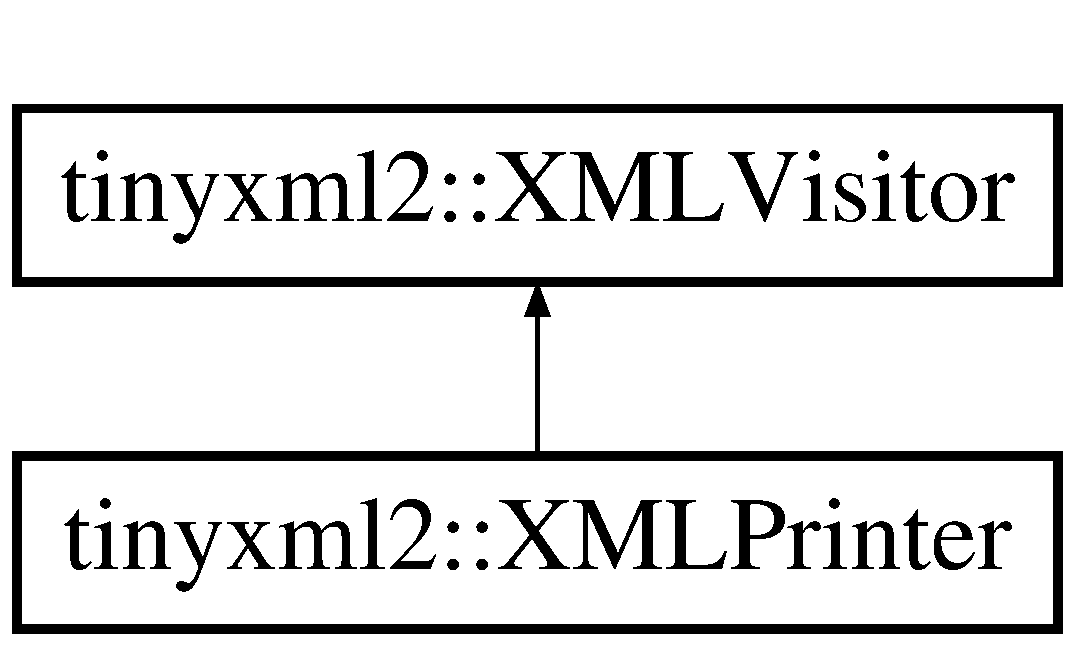
\includegraphics[height=2.000000cm]{classtinyxml2_1_1_x_m_l_printer}
\end{center}
\end{figure}
\subsection*{Public Member Functions}
\begin{DoxyCompactItemize}
\item 
\hyperlink{classtinyxml2_1_1_x_m_l_printer_aa6d3841c069085f5b8a27bc7103c04f7}{X\-M\-L\-Printer} (F\-I\-L\-E $\ast$file=0, bool compact=false, int depth=0)
\item 
void \hyperlink{classtinyxml2_1_1_x_m_l_printer_a178c608ce8476043d5d6513819cde903}{Push\-Header} (bool write\-B\-O\-M, bool write\-Declaration)
\item 
void \hyperlink{classtinyxml2_1_1_x_m_l_printer_aa10d330818dbc31b44e9ffc27618bdfb}{Open\-Element} (const char $\ast$name)
\item 
\hypertarget{classtinyxml2_1_1_x_m_l_printer_a9a4e2c9348b42e147629d5a99f4af3f0}{void \hyperlink{classtinyxml2_1_1_x_m_l_printer_a9a4e2c9348b42e147629d5a99f4af3f0}{Push\-Attribute} (const char $\ast$name, const char $\ast$value)}\label{classtinyxml2_1_1_x_m_l_printer_a9a4e2c9348b42e147629d5a99f4af3f0}

\begin{DoxyCompactList}\small\item\em If streaming, add an attribute to an open element. \end{DoxyCompactList}\item 
\hypertarget{classtinyxml2_1_1_x_m_l_printer_a69120c82088597372d28d0a98f2ee7a1}{void {\bfseries Push\-Attribute} (const char $\ast$name, int value)}\label{classtinyxml2_1_1_x_m_l_printer_a69120c82088597372d28d0a98f2ee7a1}

\item 
\hypertarget{classtinyxml2_1_1_x_m_l_printer_aa41039e51990aaf5342f3e0575a692c4}{void {\bfseries Push\-Attribute} (const char $\ast$name, unsigned value)}\label{classtinyxml2_1_1_x_m_l_printer_aa41039e51990aaf5342f3e0575a692c4}

\item 
\hypertarget{classtinyxml2_1_1_x_m_l_printer_a51f7950d7b7a19f0d3a0d549a318d45f}{void {\bfseries Push\-Attribute} (const char $\ast$name, bool value)}\label{classtinyxml2_1_1_x_m_l_printer_a51f7950d7b7a19f0d3a0d549a318d45f}

\item 
\hypertarget{classtinyxml2_1_1_x_m_l_printer_a1714867af40e68ca404c3e84b6cac2a6}{void {\bfseries Push\-Attribute} (const char $\ast$name, double value)}\label{classtinyxml2_1_1_x_m_l_printer_a1714867af40e68ca404c3e84b6cac2a6}

\item 
\hypertarget{classtinyxml2_1_1_x_m_l_printer_aed6cce4bd414a78b3e2a824803c3ec42}{virtual void \hyperlink{classtinyxml2_1_1_x_m_l_printer_aed6cce4bd414a78b3e2a824803c3ec42}{Close\-Element} ()}\label{classtinyxml2_1_1_x_m_l_printer_aed6cce4bd414a78b3e2a824803c3ec42}

\begin{DoxyCompactList}\small\item\em If streaming, close the Element. \end{DoxyCompactList}\item 
\hypertarget{classtinyxml2_1_1_x_m_l_printer_a1cc16a9362df4332012cb13cff6441b3}{void \hyperlink{classtinyxml2_1_1_x_m_l_printer_a1cc16a9362df4332012cb13cff6441b3}{Push\-Text} (const char $\ast$text, bool cdata=false)}\label{classtinyxml2_1_1_x_m_l_printer_a1cc16a9362df4332012cb13cff6441b3}

\begin{DoxyCompactList}\small\item\em Add a text node. \end{DoxyCompactList}\item 
\hypertarget{classtinyxml2_1_1_x_m_l_printer_a3e0d4d78de25d4cf081009e1431cea7e}{void \hyperlink{classtinyxml2_1_1_x_m_l_printer_a3e0d4d78de25d4cf081009e1431cea7e}{Push\-Text} (int value)}\label{classtinyxml2_1_1_x_m_l_printer_a3e0d4d78de25d4cf081009e1431cea7e}

\begin{DoxyCompactList}\small\item\em Add a text node from an integer. \end{DoxyCompactList}\item 
\hypertarget{classtinyxml2_1_1_x_m_l_printer_a661fb50e7e0a4918d2d259cb0fae647e}{void \hyperlink{classtinyxml2_1_1_x_m_l_printer_a661fb50e7e0a4918d2d259cb0fae647e}{Push\-Text} (unsigned value)}\label{classtinyxml2_1_1_x_m_l_printer_a661fb50e7e0a4918d2d259cb0fae647e}

\begin{DoxyCompactList}\small\item\em Add a text node from an unsigned. \end{DoxyCompactList}\item 
\hypertarget{classtinyxml2_1_1_x_m_l_printer_a4390e5fa1ed05189a8686647345ab29f}{void \hyperlink{classtinyxml2_1_1_x_m_l_printer_a4390e5fa1ed05189a8686647345ab29f}{Push\-Text} (bool value)}\label{classtinyxml2_1_1_x_m_l_printer_a4390e5fa1ed05189a8686647345ab29f}

\begin{DoxyCompactList}\small\item\em Add a text node from a bool. \end{DoxyCompactList}\item 
\hypertarget{classtinyxml2_1_1_x_m_l_printer_a1dbb1390e829d0673af66b9cd1928bd7}{void \hyperlink{classtinyxml2_1_1_x_m_l_printer_a1dbb1390e829d0673af66b9cd1928bd7}{Push\-Text} (float value)}\label{classtinyxml2_1_1_x_m_l_printer_a1dbb1390e829d0673af66b9cd1928bd7}

\begin{DoxyCompactList}\small\item\em Add a text node from a float. \end{DoxyCompactList}\item 
\hypertarget{classtinyxml2_1_1_x_m_l_printer_aa715302dfc09473c77c853cbd5431965}{void \hyperlink{classtinyxml2_1_1_x_m_l_printer_aa715302dfc09473c77c853cbd5431965}{Push\-Text} (double value)}\label{classtinyxml2_1_1_x_m_l_printer_aa715302dfc09473c77c853cbd5431965}

\begin{DoxyCompactList}\small\item\em Add a text node from a double. \end{DoxyCompactList}\item 
\hypertarget{classtinyxml2_1_1_x_m_l_printer_afc8416814219591c2fd5656e0c233140}{void \hyperlink{classtinyxml2_1_1_x_m_l_printer_afc8416814219591c2fd5656e0c233140}{Push\-Comment} (const char $\ast$comment)}\label{classtinyxml2_1_1_x_m_l_printer_afc8416814219591c2fd5656e0c233140}

\begin{DoxyCompactList}\small\item\em Add a comment. \end{DoxyCompactList}\item 
\hypertarget{classtinyxml2_1_1_x_m_l_printer_a2fe3565e262594efc6c0276723c83fe7}{void {\bfseries Push\-Declaration} (const char $\ast$value)}\label{classtinyxml2_1_1_x_m_l_printer_a2fe3565e262594efc6c0276723c83fe7}

\item 
\hypertarget{classtinyxml2_1_1_x_m_l_printer_ab1efc6d1548505e9984185f58f54b713}{void {\bfseries Push\-Unknown} (const char $\ast$value)}\label{classtinyxml2_1_1_x_m_l_printer_ab1efc6d1548505e9984185f58f54b713}

\item 
\hypertarget{classtinyxml2_1_1_x_m_l_printer_a9aa1de11a55a07db55a90fde37d7afad}{virtual bool \hyperlink{classtinyxml2_1_1_x_m_l_printer_a9aa1de11a55a07db55a90fde37d7afad}{Visit\-Enter} (const \hyperlink{classtinyxml2_1_1_x_m_l_document}{X\-M\-L\-Document} \&)}\label{classtinyxml2_1_1_x_m_l_printer_a9aa1de11a55a07db55a90fde37d7afad}

\begin{DoxyCompactList}\small\item\em Visit a document. \end{DoxyCompactList}\item 
\hypertarget{classtinyxml2_1_1_x_m_l_printer_a15fc1f2b922f540917dcf52808737b29}{virtual bool \hyperlink{classtinyxml2_1_1_x_m_l_printer_a15fc1f2b922f540917dcf52808737b29}{Visit\-Exit} (const \hyperlink{classtinyxml2_1_1_x_m_l_document}{X\-M\-L\-Document} \&)}\label{classtinyxml2_1_1_x_m_l_printer_a15fc1f2b922f540917dcf52808737b29}

\begin{DoxyCompactList}\small\item\em Visit a document. \end{DoxyCompactList}\item 
\hypertarget{classtinyxml2_1_1_x_m_l_printer_a169b2509d8eabb70811b2bb8cfd1f5d1}{virtual bool \hyperlink{classtinyxml2_1_1_x_m_l_printer_a169b2509d8eabb70811b2bb8cfd1f5d1}{Visit\-Enter} (const \hyperlink{classtinyxml2_1_1_x_m_l_element}{X\-M\-L\-Element} \&element, const \hyperlink{classtinyxml2_1_1_x_m_l_attribute}{X\-M\-L\-Attribute} $\ast$attribute)}\label{classtinyxml2_1_1_x_m_l_printer_a169b2509d8eabb70811b2bb8cfd1f5d1}

\begin{DoxyCompactList}\small\item\em Visit an element. \end{DoxyCompactList}\item 
\hypertarget{classtinyxml2_1_1_x_m_l_printer_a2edd48405971a88951c71c9df86a2f50}{virtual bool \hyperlink{classtinyxml2_1_1_x_m_l_printer_a2edd48405971a88951c71c9df86a2f50}{Visit\-Exit} (const \hyperlink{classtinyxml2_1_1_x_m_l_element}{X\-M\-L\-Element} \&element)}\label{classtinyxml2_1_1_x_m_l_printer_a2edd48405971a88951c71c9df86a2f50}

\begin{DoxyCompactList}\small\item\em Visit an element. \end{DoxyCompactList}\item 
\hypertarget{classtinyxml2_1_1_x_m_l_printer_adc0e42b4f6fcb90a95630c79575d030b}{virtual bool \hyperlink{classtinyxml2_1_1_x_m_l_printer_adc0e42b4f6fcb90a95630c79575d030b}{Visit} (const \hyperlink{classtinyxml2_1_1_x_m_l_text}{X\-M\-L\-Text} \&text)}\label{classtinyxml2_1_1_x_m_l_printer_adc0e42b4f6fcb90a95630c79575d030b}

\begin{DoxyCompactList}\small\item\em Visit a text node. \end{DoxyCompactList}\item 
\hypertarget{classtinyxml2_1_1_x_m_l_printer_aa294c5c01af0ebb9114902456e4cb53c}{virtual bool \hyperlink{classtinyxml2_1_1_x_m_l_printer_aa294c5c01af0ebb9114902456e4cb53c}{Visit} (const \hyperlink{classtinyxml2_1_1_x_m_l_comment}{X\-M\-L\-Comment} \&comment)}\label{classtinyxml2_1_1_x_m_l_printer_aa294c5c01af0ebb9114902456e4cb53c}

\begin{DoxyCompactList}\small\item\em Visit a comment node. \end{DoxyCompactList}\item 
\hypertarget{classtinyxml2_1_1_x_m_l_printer_acfc625b2549304b9c7eb85ebd5c5eb39}{virtual bool \hyperlink{classtinyxml2_1_1_x_m_l_printer_acfc625b2549304b9c7eb85ebd5c5eb39}{Visit} (const \hyperlink{classtinyxml2_1_1_x_m_l_declaration}{X\-M\-L\-Declaration} \&declaration)}\label{classtinyxml2_1_1_x_m_l_printer_acfc625b2549304b9c7eb85ebd5c5eb39}

\begin{DoxyCompactList}\small\item\em Visit a declaration. \end{DoxyCompactList}\item 
\hypertarget{classtinyxml2_1_1_x_m_l_printer_ab8af5455bbf9e4be2663e6642fcd7e32}{virtual bool \hyperlink{classtinyxml2_1_1_x_m_l_printer_ab8af5455bbf9e4be2663e6642fcd7e32}{Visit} (const \hyperlink{classtinyxml2_1_1_x_m_l_unknown}{X\-M\-L\-Unknown} \&unknown)}\label{classtinyxml2_1_1_x_m_l_printer_ab8af5455bbf9e4be2663e6642fcd7e32}

\begin{DoxyCompactList}\small\item\em Visit an unknown node. \end{DoxyCompactList}\item 
const char $\ast$ \hyperlink{classtinyxml2_1_1_x_m_l_printer_a4a1b788e11b540921ec50687cd2b24a9}{C\-Str} () const 
\item 
int \hyperlink{classtinyxml2_1_1_x_m_l_printer_a02c3c5f8c6c007dcbaf10595d9e22bf0}{C\-Str\-Size} () const 
\end{DoxyCompactItemize}
\subsection*{Protected Member Functions}
\begin{DoxyCompactItemize}
\item 
\hypertarget{classtinyxml2_1_1_x_m_l_printer_a70ac2010150c8551773ffb2f96fef353}{void {\bfseries Seal\-Element} ()}\label{classtinyxml2_1_1_x_m_l_printer_a70ac2010150c8551773ffb2f96fef353}

\end{DoxyCompactItemize}
\subsection*{Protected Attributes}
\begin{DoxyCompactItemize}
\item 
\hypertarget{classtinyxml2_1_1_x_m_l_printer_ac07169d58b465214a2b1fa306e617c26}{bool {\bfseries \-\_\-element\-Just\-Opened}}\label{classtinyxml2_1_1_x_m_l_printer_ac07169d58b465214a2b1fa306e617c26}

\item 
\hypertarget{classtinyxml2_1_1_x_m_l_printer_a99d59e67e084714541bee3ae43884bef}{\hyperlink{classtinyxml2_1_1_dyn_array}{Dyn\-Array}$<$ const char $\ast$, 10 $>$ {\bfseries \-\_\-stack}}\label{classtinyxml2_1_1_x_m_l_printer_a99d59e67e084714541bee3ae43884bef}

\end{DoxyCompactItemize}


\subsection{Detailed Description}
Printing functionality. The \hyperlink{classtinyxml2_1_1_x_m_l_printer}{X\-M\-L\-Printer} gives you more options than the \hyperlink{classtinyxml2_1_1_x_m_l_document_a686ea28672c0e0c60383ec28148c1ac0}{X\-M\-L\-Document\-::\-Print()} method.

It can\-:
\begin{DoxyEnumerate}
\item Print to memory.
\item Print to a file you provide.
\item Print X\-M\-L without a \hyperlink{classtinyxml2_1_1_x_m_l_document}{X\-M\-L\-Document}.
\end{DoxyEnumerate}

Print to Memory

\begin{DoxyVerb}XMLPrinter printer;
doc.Print( &printer );
SomeFunction( printer.CStr() );
\end{DoxyVerb}


Print to a File

You provide the file pointer. \begin{DoxyVerb}XMLPrinter printer( fp );
doc.Print( &printer );
\end{DoxyVerb}


Print without a \hyperlink{classtinyxml2_1_1_x_m_l_document}{X\-M\-L\-Document}

When loading, an X\-M\-L parser is very useful. However, sometimes when saving, it just gets in the way. The code is often set up for streaming, and constructing the D\-O\-M is just overhead.

The Printer supports the streaming case. The following code prints out a trivially simple X\-M\-L file without ever creating an X\-M\-L document.

\begin{DoxyVerb}XMLPrinter printer( fp );
printer.OpenElement( "foo" );
printer.PushAttribute( "foo", "bar" );
printer.CloseElement();
\end{DoxyVerb}
 

\subsection{Constructor \& Destructor Documentation}
\hypertarget{classtinyxml2_1_1_x_m_l_printer_aa6d3841c069085f5b8a27bc7103c04f7}{\index{tinyxml2\-::\-X\-M\-L\-Printer@{tinyxml2\-::\-X\-M\-L\-Printer}!X\-M\-L\-Printer@{X\-M\-L\-Printer}}
\index{X\-M\-L\-Printer@{X\-M\-L\-Printer}!tinyxml2::XMLPrinter@{tinyxml2\-::\-X\-M\-L\-Printer}}
\subsubsection[{X\-M\-L\-Printer}]{\setlength{\rightskip}{0pt plus 5cm}tinyxml2\-::\-X\-M\-L\-Printer\-::\-X\-M\-L\-Printer (
\begin{DoxyParamCaption}
\item[{F\-I\-L\-E $\ast$}]{file = {\ttfamily 0}, }
\item[{bool}]{compact = {\ttfamily false}, }
\item[{int}]{depth = {\ttfamily 0}}
\end{DoxyParamCaption}
)}}\label{classtinyxml2_1_1_x_m_l_printer_aa6d3841c069085f5b8a27bc7103c04f7}
Construct the printer. If the F\-I\-L\-E$\ast$ is specified, this will print to the F\-I\-L\-E. Else it will print to memory, and the result is available in \hyperlink{classtinyxml2_1_1_x_m_l_printer_a4a1b788e11b540921ec50687cd2b24a9}{C\-Str()}. If 'compact' is set to true, then output is created with only required whitespace and newlines. 

\subsection{Member Function Documentation}
\hypertarget{classtinyxml2_1_1_x_m_l_printer_a4a1b788e11b540921ec50687cd2b24a9}{\index{tinyxml2\-::\-X\-M\-L\-Printer@{tinyxml2\-::\-X\-M\-L\-Printer}!C\-Str@{C\-Str}}
\index{C\-Str@{C\-Str}!tinyxml2::XMLPrinter@{tinyxml2\-::\-X\-M\-L\-Printer}}
\subsubsection[{C\-Str}]{\setlength{\rightskip}{0pt plus 5cm}const char$\ast$ tinyxml2\-::\-X\-M\-L\-Printer\-::\-C\-Str (
\begin{DoxyParamCaption}
{}
\end{DoxyParamCaption}
) const\hspace{0.3cm}{\ttfamily [inline]}}}\label{classtinyxml2_1_1_x_m_l_printer_a4a1b788e11b540921ec50687cd2b24a9}
If in print to memory mode, return a pointer to the X\-M\-L file in memory. \hypertarget{classtinyxml2_1_1_x_m_l_printer_a02c3c5f8c6c007dcbaf10595d9e22bf0}{\index{tinyxml2\-::\-X\-M\-L\-Printer@{tinyxml2\-::\-X\-M\-L\-Printer}!C\-Str\-Size@{C\-Str\-Size}}
\index{C\-Str\-Size@{C\-Str\-Size}!tinyxml2::XMLPrinter@{tinyxml2\-::\-X\-M\-L\-Printer}}
\subsubsection[{C\-Str\-Size}]{\setlength{\rightskip}{0pt plus 5cm}int tinyxml2\-::\-X\-M\-L\-Printer\-::\-C\-Str\-Size (
\begin{DoxyParamCaption}
{}
\end{DoxyParamCaption}
) const\hspace{0.3cm}{\ttfamily [inline]}}}\label{classtinyxml2_1_1_x_m_l_printer_a02c3c5f8c6c007dcbaf10595d9e22bf0}
If in print to memory mode, return the size of the X\-M\-L file in memory. (Note the size returned includes the terminating null.) \hypertarget{classtinyxml2_1_1_x_m_l_printer_aa10d330818dbc31b44e9ffc27618bdfb}{\index{tinyxml2\-::\-X\-M\-L\-Printer@{tinyxml2\-::\-X\-M\-L\-Printer}!Open\-Element@{Open\-Element}}
\index{Open\-Element@{Open\-Element}!tinyxml2::XMLPrinter@{tinyxml2\-::\-X\-M\-L\-Printer}}
\subsubsection[{Open\-Element}]{\setlength{\rightskip}{0pt plus 5cm}void tinyxml2\-::\-X\-M\-L\-Printer\-::\-Open\-Element (
\begin{DoxyParamCaption}
\item[{const char $\ast$}]{name}
\end{DoxyParamCaption}
)}}\label{classtinyxml2_1_1_x_m_l_printer_aa10d330818dbc31b44e9ffc27618bdfb}
If streaming, start writing an element. The element must be closed with \hyperlink{classtinyxml2_1_1_x_m_l_printer_aed6cce4bd414a78b3e2a824803c3ec42}{Close\-Element()} \hypertarget{classtinyxml2_1_1_x_m_l_printer_a178c608ce8476043d5d6513819cde903}{\index{tinyxml2\-::\-X\-M\-L\-Printer@{tinyxml2\-::\-X\-M\-L\-Printer}!Push\-Header@{Push\-Header}}
\index{Push\-Header@{Push\-Header}!tinyxml2::XMLPrinter@{tinyxml2\-::\-X\-M\-L\-Printer}}
\subsubsection[{Push\-Header}]{\setlength{\rightskip}{0pt plus 5cm}void tinyxml2\-::\-X\-M\-L\-Printer\-::\-Push\-Header (
\begin{DoxyParamCaption}
\item[{bool}]{write\-B\-O\-M, }
\item[{bool}]{write\-Declaration}
\end{DoxyParamCaption}
)}}\label{classtinyxml2_1_1_x_m_l_printer_a178c608ce8476043d5d6513819cde903}
If streaming, write the B\-O\-M and declaration. 

The documentation for this class was generated from the following files\-:\begin{DoxyCompactItemize}
\item 
Joes\-\_\-\-S\-D\-L\-\_\-\-Framework/tinyxml2.\-h\item 
Joes\-\_\-\-S\-D\-L\-\_\-\-Framework/tinyxml2.\-cpp\end{DoxyCompactItemize}

\hypertarget{classtinyxml2_1_1_x_m_l_text}{\section{tinyxml2\-:\-:X\-M\-L\-Text Class Reference}
\label{classtinyxml2_1_1_x_m_l_text}\index{tinyxml2\-::\-X\-M\-L\-Text@{tinyxml2\-::\-X\-M\-L\-Text}}
}


{\ttfamily \#include $<$tinyxml2.\-h$>$}

Inheritance diagram for tinyxml2\-:\-:X\-M\-L\-Text\-:\begin{figure}[H]
\begin{center}
\leavevmode
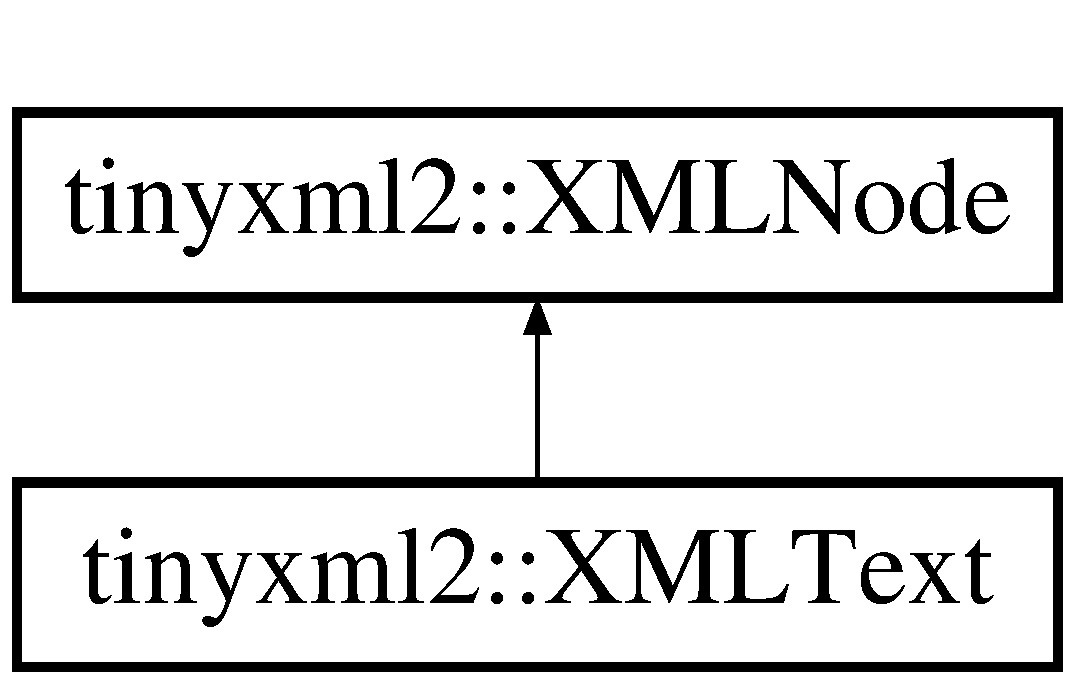
\includegraphics[height=2.000000cm]{classtinyxml2_1_1_x_m_l_text}
\end{center}
\end{figure}
\subsection*{Public Member Functions}
\begin{DoxyCompactItemize}
\item 
virtual bool \hyperlink{classtinyxml2_1_1_x_m_l_text_ae659d4fc7351a7df11c111cbe1ade46f}{Accept} (\hyperlink{classtinyxml2_1_1_x_m_l_visitor}{X\-M\-L\-Visitor} $\ast$visitor) const 
\item 
\hypertarget{classtinyxml2_1_1_x_m_l_text_ab1213b4ddebe9b17ec7e7040e9f1caf7}{virtual \hyperlink{classtinyxml2_1_1_x_m_l_text}{X\-M\-L\-Text} $\ast$ \hyperlink{classtinyxml2_1_1_x_m_l_text_ab1213b4ddebe9b17ec7e7040e9f1caf7}{To\-Text} ()}\label{classtinyxml2_1_1_x_m_l_text_ab1213b4ddebe9b17ec7e7040e9f1caf7}

\begin{DoxyCompactList}\small\item\em Safely cast to Text, or null. \end{DoxyCompactList}\item 
\hypertarget{classtinyxml2_1_1_x_m_l_text_a1e53cbc60968fe966790a65eaf87baaa}{virtual const \hyperlink{classtinyxml2_1_1_x_m_l_text}{X\-M\-L\-Text} $\ast$ {\bfseries To\-Text} () const }\label{classtinyxml2_1_1_x_m_l_text_a1e53cbc60968fe966790a65eaf87baaa}

\item 
\hypertarget{classtinyxml2_1_1_x_m_l_text_ad080357d76ab7cc59d7651249949329d}{void \hyperlink{classtinyxml2_1_1_x_m_l_text_ad080357d76ab7cc59d7651249949329d}{Set\-C\-Data} (bool is\-C\-Data)}\label{classtinyxml2_1_1_x_m_l_text_ad080357d76ab7cc59d7651249949329d}

\begin{DoxyCompactList}\small\item\em Declare whether this should be C\-D\-A\-T\-A or standard text. \end{DoxyCompactList}\item 
\hypertarget{classtinyxml2_1_1_x_m_l_text_a125574fe49da80efbae1349f20d02d41}{bool \hyperlink{classtinyxml2_1_1_x_m_l_text_a125574fe49da80efbae1349f20d02d41}{C\-Data} () const }\label{classtinyxml2_1_1_x_m_l_text_a125574fe49da80efbae1349f20d02d41}

\begin{DoxyCompactList}\small\item\em Returns true if this is a C\-D\-A\-T\-A text element. \end{DoxyCompactList}\item 
\hypertarget{classtinyxml2_1_1_x_m_l_text_ac18d9eec9f12b827b0d02b0847bf279e}{char $\ast$ {\bfseries Parse\-Deep} (char $\ast$, \hyperlink{classtinyxml2_1_1_str_pair}{Str\-Pair} $\ast$end\-Tag)}\label{classtinyxml2_1_1_x_m_l_text_ac18d9eec9f12b827b0d02b0847bf279e}

\item 
virtual \hyperlink{classtinyxml2_1_1_x_m_l_node}{X\-M\-L\-Node} $\ast$ \hyperlink{classtinyxml2_1_1_x_m_l_text_af5115f8cc83de2947ed6a9d13e2f88c8}{Shallow\-Clone} (\hyperlink{classtinyxml2_1_1_x_m_l_document}{X\-M\-L\-Document} $\ast$document) const 
\item 
virtual bool \hyperlink{classtinyxml2_1_1_x_m_l_text_a1588aa5d23cb21eb31f36df0aaaa8d66}{Shallow\-Equal} (const \hyperlink{classtinyxml2_1_1_x_m_l_node}{X\-M\-L\-Node} $\ast$compare) const 
\end{DoxyCompactItemize}
\subsection*{Protected Member Functions}
\begin{DoxyCompactItemize}
\item 
\hypertarget{classtinyxml2_1_1_x_m_l_text_ad9f46d70e61e5386ead93728d8b90267}{{\bfseries X\-M\-L\-Text} (\hyperlink{classtinyxml2_1_1_x_m_l_document}{X\-M\-L\-Document} $\ast$doc)}\label{classtinyxml2_1_1_x_m_l_text_ad9f46d70e61e5386ead93728d8b90267}

\item 
\hypertarget{classtinyxml2_1_1_x_m_l_text_a002156e1f61ee6d48e5368b7cca25582}{{\bfseries X\-M\-L\-Text} (const \hyperlink{classtinyxml2_1_1_x_m_l_text}{X\-M\-L\-Text} \&)}\label{classtinyxml2_1_1_x_m_l_text_a002156e1f61ee6d48e5368b7cca25582}

\item 
\hypertarget{classtinyxml2_1_1_x_m_l_text_ad8c9f398d92fa472e213b89d8483ae8f}{\hyperlink{classtinyxml2_1_1_x_m_l_text}{X\-M\-L\-Text} \& {\bfseries operator=} (const \hyperlink{classtinyxml2_1_1_x_m_l_text}{X\-M\-L\-Text} \&)}\label{classtinyxml2_1_1_x_m_l_text_ad8c9f398d92fa472e213b89d8483ae8f}

\end{DoxyCompactItemize}
\subsection*{Friends}
\begin{DoxyCompactItemize}
\item 
\hypertarget{classtinyxml2_1_1_x_m_l_text_a449202cfc89e7ae5c2f81995476f9ec1}{class {\bfseries X\-M\-L\-Base}}\label{classtinyxml2_1_1_x_m_l_text_a449202cfc89e7ae5c2f81995476f9ec1}

\item 
\hypertarget{classtinyxml2_1_1_x_m_l_text_a4eee3bda60c60a30e4e8cd4ea91c4c6e}{class {\bfseries X\-M\-L\-Document}}\label{classtinyxml2_1_1_x_m_l_text_a4eee3bda60c60a30e4e8cd4ea91c4c6e}

\end{DoxyCompactItemize}
\subsection*{Additional Inherited Members}


\subsection{Detailed Description}
X\-M\-L text.

Note that a text node can have child element nodes, for example\-: \begin{DoxyVerb}<root>This is <b>bold</b></root>
\end{DoxyVerb}


A text node can have 2 ways to output the next. \char`\"{}normal\char`\"{} output and C\-D\-A\-T\-A. It will default to the mode it was parsed from the X\-M\-L file and you generally want to leave it alone, but you can change the output mode with \hyperlink{classtinyxml2_1_1_x_m_l_text_ad080357d76ab7cc59d7651249949329d}{Set\-C\-Data()} and query it with \hyperlink{classtinyxml2_1_1_x_m_l_text_a125574fe49da80efbae1349f20d02d41}{C\-Data()}. 

\subsection{Member Function Documentation}
\hypertarget{classtinyxml2_1_1_x_m_l_text_ae659d4fc7351a7df11c111cbe1ade46f}{\index{tinyxml2\-::\-X\-M\-L\-Text@{tinyxml2\-::\-X\-M\-L\-Text}!Accept@{Accept}}
\index{Accept@{Accept}!tinyxml2::XMLText@{tinyxml2\-::\-X\-M\-L\-Text}}
\subsubsection[{Accept}]{\setlength{\rightskip}{0pt plus 5cm}bool tinyxml2\-::\-X\-M\-L\-Text\-::\-Accept (
\begin{DoxyParamCaption}
\item[{{\bf X\-M\-L\-Visitor} $\ast$}]{visitor}
\end{DoxyParamCaption}
) const\hspace{0.3cm}{\ttfamily [virtual]}}}\label{classtinyxml2_1_1_x_m_l_text_ae659d4fc7351a7df11c111cbe1ade46f}
Accept a hierarchical visit of the nodes in the Tiny\-X\-M\-L-\/2 D\-O\-M. Every node in the X\-M\-L tree will be conditionally visited and the host will be called back via the \hyperlink{classtinyxml2_1_1_x_m_l_visitor}{X\-M\-L\-Visitor} interface.

This is essentially a S\-A\-X interface for Tiny\-X\-M\-L-\/2. (Note however it doesn't re-\/parse the X\-M\-L for the callbacks, so the performance of Tiny\-X\-M\-L-\/2 is unchanged by using this interface versus any other.)

The interface has been based on ideas from\-:


\begin{DoxyItemize}
\item \href{http://www.saxproject.org/}{\tt http\-://www.\-saxproject.\-org/}
\item \href{http://c2.com/cgi/wiki?HierarchicalVisitorPattern}{\tt http\-://c2.\-com/cgi/wiki?\-Hierarchical\-Visitor\-Pattern}
\end{DoxyItemize}

Which are both good references for \char`\"{}visiting\char`\"{}.

An example of using \hyperlink{classtinyxml2_1_1_x_m_l_text_ae659d4fc7351a7df11c111cbe1ade46f}{Accept()}\-: \begin{DoxyVerb}XMLPrinter printer;
tinyxmlDoc.Accept( &printer );
const char* xmlcstr = printer.CStr();
\end{DoxyVerb}
 

Implements \hyperlink{classtinyxml2_1_1_x_m_l_node_a81e66df0a44c67a7af17f3b77a152785}{tinyxml2\-::\-X\-M\-L\-Node}.

\hypertarget{classtinyxml2_1_1_x_m_l_text_af5115f8cc83de2947ed6a9d13e2f88c8}{\index{tinyxml2\-::\-X\-M\-L\-Text@{tinyxml2\-::\-X\-M\-L\-Text}!Shallow\-Clone@{Shallow\-Clone}}
\index{Shallow\-Clone@{Shallow\-Clone}!tinyxml2::XMLText@{tinyxml2\-::\-X\-M\-L\-Text}}
\subsubsection[{Shallow\-Clone}]{\setlength{\rightskip}{0pt plus 5cm}{\bf X\-M\-L\-Node} $\ast$ tinyxml2\-::\-X\-M\-L\-Text\-::\-Shallow\-Clone (
\begin{DoxyParamCaption}
\item[{{\bf X\-M\-L\-Document} $\ast$}]{document}
\end{DoxyParamCaption}
) const\hspace{0.3cm}{\ttfamily [virtual]}}}\label{classtinyxml2_1_1_x_m_l_text_af5115f8cc83de2947ed6a9d13e2f88c8}
Make a copy of this node, but not its children. You may pass in a Document pointer that will be the owner of the new Node. If the 'document' is null, then the node returned will be allocated from the current Document. (this-\/$>$\hyperlink{classtinyxml2_1_1_x_m_l_node_af343d1ef0b45c0020e62d784d7e67a68}{Get\-Document()})

Note\-: if called on a \hyperlink{classtinyxml2_1_1_x_m_l_document}{X\-M\-L\-Document}, this will return null. 

Implements \hyperlink{classtinyxml2_1_1_x_m_l_node_a8402cbd3129d20e9e6024bbcc0531283}{tinyxml2\-::\-X\-M\-L\-Node}.

\hypertarget{classtinyxml2_1_1_x_m_l_text_a1588aa5d23cb21eb31f36df0aaaa8d66}{\index{tinyxml2\-::\-X\-M\-L\-Text@{tinyxml2\-::\-X\-M\-L\-Text}!Shallow\-Equal@{Shallow\-Equal}}
\index{Shallow\-Equal@{Shallow\-Equal}!tinyxml2::XMLText@{tinyxml2\-::\-X\-M\-L\-Text}}
\subsubsection[{Shallow\-Equal}]{\setlength{\rightskip}{0pt plus 5cm}bool tinyxml2\-::\-X\-M\-L\-Text\-::\-Shallow\-Equal (
\begin{DoxyParamCaption}
\item[{const {\bf X\-M\-L\-Node} $\ast$}]{compare}
\end{DoxyParamCaption}
) const\hspace{0.3cm}{\ttfamily [virtual]}}}\label{classtinyxml2_1_1_x_m_l_text_a1588aa5d23cb21eb31f36df0aaaa8d66}
Test if 2 nodes are the same, but don't test children. The 2 nodes do not need to be in the same Document.

Note\-: if called on a \hyperlink{classtinyxml2_1_1_x_m_l_document}{X\-M\-L\-Document}, this will return false. 

Implements \hyperlink{classtinyxml2_1_1_x_m_l_node_a7ce18b751c3ea09eac292dca264f9226}{tinyxml2\-::\-X\-M\-L\-Node}.



The documentation for this class was generated from the following files\-:\begin{DoxyCompactItemize}
\item 
Joes\-\_\-\-S\-D\-L\-\_\-\-Framework/tinyxml2.\-h\item 
Joes\-\_\-\-S\-D\-L\-\_\-\-Framework/tinyxml2.\-cpp\end{DoxyCompactItemize}

\hypertarget{classtinyxml2_1_1_x_m_l_unknown}{\section{tinyxml2\-:\-:X\-M\-L\-Unknown Class Reference}
\label{classtinyxml2_1_1_x_m_l_unknown}\index{tinyxml2\-::\-X\-M\-L\-Unknown@{tinyxml2\-::\-X\-M\-L\-Unknown}}
}


{\ttfamily \#include $<$tinyxml2.\-h$>$}

Inheritance diagram for tinyxml2\-:\-:X\-M\-L\-Unknown\-:\begin{figure}[H]
\begin{center}
\leavevmode
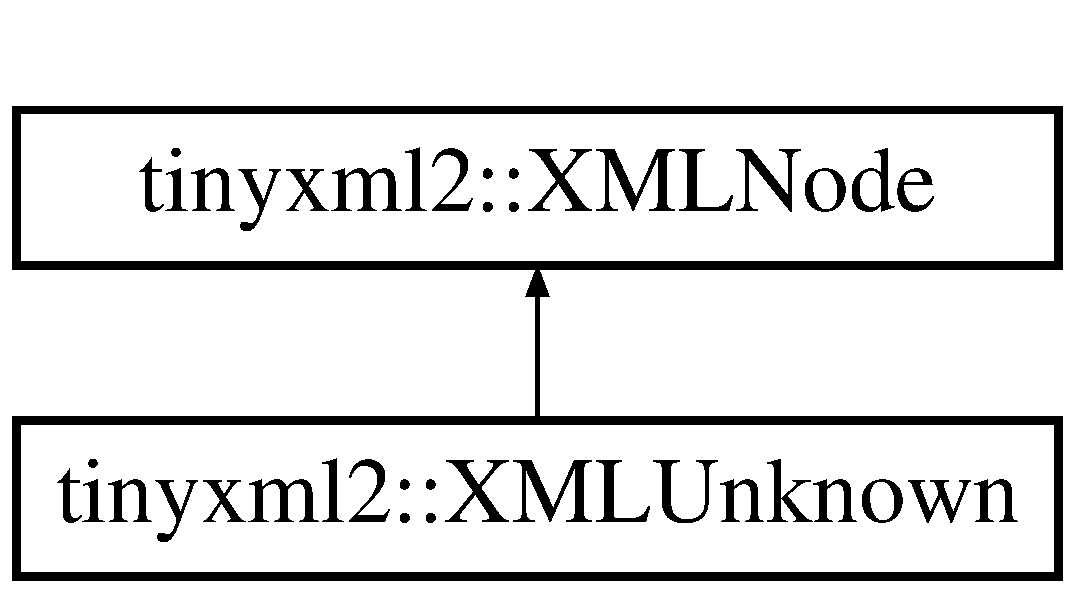
\includegraphics[height=2.000000cm]{classtinyxml2_1_1_x_m_l_unknown}
\end{center}
\end{figure}
\subsection*{Public Member Functions}
\begin{DoxyCompactItemize}
\item 
\hypertarget{classtinyxml2_1_1_x_m_l_unknown_af4374856421921cad578c8affae872b6}{virtual \hyperlink{classtinyxml2_1_1_x_m_l_unknown}{X\-M\-L\-Unknown} $\ast$ \hyperlink{classtinyxml2_1_1_x_m_l_unknown_af4374856421921cad578c8affae872b6}{To\-Unknown} ()}\label{classtinyxml2_1_1_x_m_l_unknown_af4374856421921cad578c8affae872b6}

\begin{DoxyCompactList}\small\item\em Safely cast to an Unknown, or null. \end{DoxyCompactList}\item 
\hypertarget{classtinyxml2_1_1_x_m_l_unknown_a257987e79955399e6e9f119b58d4bb30}{virtual const \hyperlink{classtinyxml2_1_1_x_m_l_unknown}{X\-M\-L\-Unknown} $\ast$ {\bfseries To\-Unknown} () const }\label{classtinyxml2_1_1_x_m_l_unknown_a257987e79955399e6e9f119b58d4bb30}

\item 
virtual bool \hyperlink{classtinyxml2_1_1_x_m_l_unknown_a0d341ab804a1438a474810bb5bd29dd5}{Accept} (\hyperlink{classtinyxml2_1_1_x_m_l_visitor}{X\-M\-L\-Visitor} $\ast$visitor) const 
\item 
\hypertarget{classtinyxml2_1_1_x_m_l_unknown_a0e4f3509dee42a4d45a7f0002be568cc}{char $\ast$ {\bfseries Parse\-Deep} (char $\ast$, \hyperlink{classtinyxml2_1_1_str_pair}{Str\-Pair} $\ast$end\-Tag)}\label{classtinyxml2_1_1_x_m_l_unknown_a0e4f3509dee42a4d45a7f0002be568cc}

\item 
virtual \hyperlink{classtinyxml2_1_1_x_m_l_node}{X\-M\-L\-Node} $\ast$ \hyperlink{classtinyxml2_1_1_x_m_l_unknown_aa09fc7cb0cd64d6bb9c5ae00ffc549ec}{Shallow\-Clone} (\hyperlink{classtinyxml2_1_1_x_m_l_document}{X\-M\-L\-Document} $\ast$document) const 
\item 
virtual bool \hyperlink{classtinyxml2_1_1_x_m_l_unknown_a0169df157bf69a092b404ca49621ff1a}{Shallow\-Equal} (const \hyperlink{classtinyxml2_1_1_x_m_l_node}{X\-M\-L\-Node} $\ast$compare) const 
\end{DoxyCompactItemize}
\subsection*{Protected Member Functions}
\begin{DoxyCompactItemize}
\item 
\hypertarget{classtinyxml2_1_1_x_m_l_unknown_a9391eb679598d50baba424e6f1aa367b}{{\bfseries X\-M\-L\-Unknown} (\hyperlink{classtinyxml2_1_1_x_m_l_document}{X\-M\-L\-Document} $\ast$doc)}\label{classtinyxml2_1_1_x_m_l_unknown_a9391eb679598d50baba424e6f1aa367b}

\item 
\hypertarget{classtinyxml2_1_1_x_m_l_unknown_aab31a93c95a7cedc9597cea7caffa73f}{{\bfseries X\-M\-L\-Unknown} (const \hyperlink{classtinyxml2_1_1_x_m_l_unknown}{X\-M\-L\-Unknown} \&)}\label{classtinyxml2_1_1_x_m_l_unknown_aab31a93c95a7cedc9597cea7caffa73f}

\item 
\hypertarget{classtinyxml2_1_1_x_m_l_unknown_a6137d5611db42c35de3d869f66555e5b}{\hyperlink{classtinyxml2_1_1_x_m_l_unknown}{X\-M\-L\-Unknown} \& {\bfseries operator=} (const \hyperlink{classtinyxml2_1_1_x_m_l_unknown}{X\-M\-L\-Unknown} \&)}\label{classtinyxml2_1_1_x_m_l_unknown_a6137d5611db42c35de3d869f66555e5b}

\end{DoxyCompactItemize}
\subsection*{Friends}
\begin{DoxyCompactItemize}
\item 
\hypertarget{classtinyxml2_1_1_x_m_l_unknown_a4eee3bda60c60a30e4e8cd4ea91c4c6e}{class {\bfseries X\-M\-L\-Document}}\label{classtinyxml2_1_1_x_m_l_unknown_a4eee3bda60c60a30e4e8cd4ea91c4c6e}

\end{DoxyCompactItemize}
\subsection*{Additional Inherited Members}


\subsection{Detailed Description}
Any tag that Tiny\-X\-M\-L-\/2 doesn't recognize is saved as an unknown. It is a tag of text, but should not be modified. It will be written back to the X\-M\-L, unchanged, when the file is saved.

D\-T\-D tags get thrown into X\-M\-L\-Unknowns. 

\subsection{Member Function Documentation}
\hypertarget{classtinyxml2_1_1_x_m_l_unknown_a0d341ab804a1438a474810bb5bd29dd5}{\index{tinyxml2\-::\-X\-M\-L\-Unknown@{tinyxml2\-::\-X\-M\-L\-Unknown}!Accept@{Accept}}
\index{Accept@{Accept}!tinyxml2::XMLUnknown@{tinyxml2\-::\-X\-M\-L\-Unknown}}
\subsubsection[{Accept}]{\setlength{\rightskip}{0pt plus 5cm}bool tinyxml2\-::\-X\-M\-L\-Unknown\-::\-Accept (
\begin{DoxyParamCaption}
\item[{{\bf X\-M\-L\-Visitor} $\ast$}]{visitor}
\end{DoxyParamCaption}
) const\hspace{0.3cm}{\ttfamily [virtual]}}}\label{classtinyxml2_1_1_x_m_l_unknown_a0d341ab804a1438a474810bb5bd29dd5}
Accept a hierarchical visit of the nodes in the Tiny\-X\-M\-L-\/2 D\-O\-M. Every node in the X\-M\-L tree will be conditionally visited and the host will be called back via the \hyperlink{classtinyxml2_1_1_x_m_l_visitor}{X\-M\-L\-Visitor} interface.

This is essentially a S\-A\-X interface for Tiny\-X\-M\-L-\/2. (Note however it doesn't re-\/parse the X\-M\-L for the callbacks, so the performance of Tiny\-X\-M\-L-\/2 is unchanged by using this interface versus any other.)

The interface has been based on ideas from\-:


\begin{DoxyItemize}
\item \href{http://www.saxproject.org/}{\tt http\-://www.\-saxproject.\-org/}
\item \href{http://c2.com/cgi/wiki?HierarchicalVisitorPattern}{\tt http\-://c2.\-com/cgi/wiki?\-Hierarchical\-Visitor\-Pattern}
\end{DoxyItemize}

Which are both good references for \char`\"{}visiting\char`\"{}.

An example of using \hyperlink{classtinyxml2_1_1_x_m_l_unknown_a0d341ab804a1438a474810bb5bd29dd5}{Accept()}\-: \begin{DoxyVerb}XMLPrinter printer;
tinyxmlDoc.Accept( &printer );
const char* xmlcstr = printer.CStr();
\end{DoxyVerb}
 

Implements \hyperlink{classtinyxml2_1_1_x_m_l_node_a81e66df0a44c67a7af17f3b77a152785}{tinyxml2\-::\-X\-M\-L\-Node}.

\hypertarget{classtinyxml2_1_1_x_m_l_unknown_aa09fc7cb0cd64d6bb9c5ae00ffc549ec}{\index{tinyxml2\-::\-X\-M\-L\-Unknown@{tinyxml2\-::\-X\-M\-L\-Unknown}!Shallow\-Clone@{Shallow\-Clone}}
\index{Shallow\-Clone@{Shallow\-Clone}!tinyxml2::XMLUnknown@{tinyxml2\-::\-X\-M\-L\-Unknown}}
\subsubsection[{Shallow\-Clone}]{\setlength{\rightskip}{0pt plus 5cm}{\bf X\-M\-L\-Node} $\ast$ tinyxml2\-::\-X\-M\-L\-Unknown\-::\-Shallow\-Clone (
\begin{DoxyParamCaption}
\item[{{\bf X\-M\-L\-Document} $\ast$}]{document}
\end{DoxyParamCaption}
) const\hspace{0.3cm}{\ttfamily [virtual]}}}\label{classtinyxml2_1_1_x_m_l_unknown_aa09fc7cb0cd64d6bb9c5ae00ffc549ec}
Make a copy of this node, but not its children. You may pass in a Document pointer that will be the owner of the new Node. If the 'document' is null, then the node returned will be allocated from the current Document. (this-\/$>$\hyperlink{classtinyxml2_1_1_x_m_l_node_af343d1ef0b45c0020e62d784d7e67a68}{Get\-Document()})

Note\-: if called on a \hyperlink{classtinyxml2_1_1_x_m_l_document}{X\-M\-L\-Document}, this will return null. 

Implements \hyperlink{classtinyxml2_1_1_x_m_l_node_a8402cbd3129d20e9e6024bbcc0531283}{tinyxml2\-::\-X\-M\-L\-Node}.

\hypertarget{classtinyxml2_1_1_x_m_l_unknown_a0169df157bf69a092b404ca49621ff1a}{\index{tinyxml2\-::\-X\-M\-L\-Unknown@{tinyxml2\-::\-X\-M\-L\-Unknown}!Shallow\-Equal@{Shallow\-Equal}}
\index{Shallow\-Equal@{Shallow\-Equal}!tinyxml2::XMLUnknown@{tinyxml2\-::\-X\-M\-L\-Unknown}}
\subsubsection[{Shallow\-Equal}]{\setlength{\rightskip}{0pt plus 5cm}bool tinyxml2\-::\-X\-M\-L\-Unknown\-::\-Shallow\-Equal (
\begin{DoxyParamCaption}
\item[{const {\bf X\-M\-L\-Node} $\ast$}]{compare}
\end{DoxyParamCaption}
) const\hspace{0.3cm}{\ttfamily [virtual]}}}\label{classtinyxml2_1_1_x_m_l_unknown_a0169df157bf69a092b404ca49621ff1a}
Test if 2 nodes are the same, but don't test children. The 2 nodes do not need to be in the same Document.

Note\-: if called on a \hyperlink{classtinyxml2_1_1_x_m_l_document}{X\-M\-L\-Document}, this will return false. 

Implements \hyperlink{classtinyxml2_1_1_x_m_l_node_a7ce18b751c3ea09eac292dca264f9226}{tinyxml2\-::\-X\-M\-L\-Node}.



The documentation for this class was generated from the following files\-:\begin{DoxyCompactItemize}
\item 
Joes\-\_\-\-S\-D\-L\-\_\-\-Framework/tinyxml2.\-h\item 
Joes\-\_\-\-S\-D\-L\-\_\-\-Framework/tinyxml2.\-cpp\end{DoxyCompactItemize}

\hypertarget{classtinyxml2_1_1_x_m_l_util}{\section{tinyxml2\-:\-:X\-M\-L\-Util Class Reference}
\label{classtinyxml2_1_1_x_m_l_util}\index{tinyxml2\-::\-X\-M\-L\-Util@{tinyxml2\-::\-X\-M\-L\-Util}}
}


{\ttfamily \#include $<$tinyxml2.\-h$>$}

\subsection*{Static Public Member Functions}
\begin{DoxyCompactItemize}
\item 
static const char $\ast$ \hyperlink{classtinyxml2_1_1_x_m_l_util_a9333d20f2a34325b5115ca45849c4b2a}{Skip\-White\-Space} (const char $\ast$p)
\item 
static char $\ast$ \hyperlink{classtinyxml2_1_1_x_m_l_util_aa48025be8843ec5a79b65579d31bd8fc}{Skip\-White\-Space} (char $\ast$p)
\item 
static bool \hyperlink{classtinyxml2_1_1_x_m_l_util_a357ec3af8fc433d19023a815f45e8e33}{Is\-White\-Space} (char p)
\item 
static bool \hyperlink{classtinyxml2_1_1_x_m_l_util_abe106a69ac4d942a4381a4d9dfd0e0bd}{Is\-Name\-Start\-Char} (unsigned char ch)
\item 
static bool \hyperlink{classtinyxml2_1_1_x_m_l_util_a04b17341538fa11752f24b4301d19485}{Is\-Name\-Char} (unsigned char ch)
\item 
static bool \hyperlink{classtinyxml2_1_1_x_m_l_util_acfcd287cacfd2533e1bc9ea4dfb56602}{String\-Equal} (const char $\ast$p, const char $\ast$q, int n\-Char=I\-N\-T\-\_\-\-M\-A\-X)
\item 
static int \hyperlink{classtinyxml2_1_1_x_m_l_util_a24ba87b1d22528167a3d16c4f52096bf}{Is\-U\-T\-F8\-Continuation} (const char p)
\item 
static const char $\ast$ \hyperlink{classtinyxml2_1_1_x_m_l_util_ae9bcb2bc3cd6475fdc644c8c17790555}{Read\-B\-O\-M} (const char $\ast$p, bool $\ast$has\-B\-O\-M)
\item 
static const char $\ast$ \hyperlink{classtinyxml2_1_1_x_m_l_util_a5a96e5144a8d693dc4bcd783d9964648}{Get\-Character\-Ref} (const char $\ast$p, char $\ast$value, int $\ast$length)
\item 
static void \hyperlink{classtinyxml2_1_1_x_m_l_util_a31c00d5c5dfb38382de1dfcaf4be3595}{Convert\-U\-T\-F32\-To\-U\-T\-F8} (unsigned long input, char $\ast$output, int $\ast$length)
\item 
static void \hyperlink{classtinyxml2_1_1_x_m_l_util_a3cd6c703d49b9d51bdf0f4ff6aa021c7}{To\-Str} (int v, char $\ast$buffer, int buffer\-Size)
\item 
static void \hyperlink{classtinyxml2_1_1_x_m_l_util_ac00c2e52c1c36dab3ff41d86a9bf60f9}{To\-Str} (unsigned v, char $\ast$buffer, int buffer\-Size)
\item 
static void \hyperlink{classtinyxml2_1_1_x_m_l_util_adba0718527ae9e80f663a71ea325cb11}{To\-Str} (bool v, char $\ast$buffer, int buffer\-Size)
\item 
static void \hyperlink{classtinyxml2_1_1_x_m_l_util_a8957ad44fee5fa02ba52d73aad4d0a31}{To\-Str} (float v, char $\ast$buffer, int buffer\-Size)
\item 
static void \hyperlink{classtinyxml2_1_1_x_m_l_util_a1cd141e50980fcddd6bf9af5de4b1db7}{To\-Str} (double v, char $\ast$buffer, int buffer\-Size)
\item 
static bool \hyperlink{classtinyxml2_1_1_x_m_l_util_ad4df4023d11ee3fca9689c49b9707323}{To\-Int} (const char $\ast$str, int $\ast$value)
\item 
static bool \hyperlink{classtinyxml2_1_1_x_m_l_util_a210c8637d5eb4ce3d4625294af0efc2f}{To\-Unsigned} (const char $\ast$str, unsigned $\ast$value)
\item 
static bool \hyperlink{classtinyxml2_1_1_x_m_l_util_ae5b03e0a1ca5d42052a7ac540f7aa12a}{To\-Bool} (const char $\ast$str, bool $\ast$value)
\item 
static bool \hyperlink{classtinyxml2_1_1_x_m_l_util_a399e71edb5f29d61ea81d91ee0332bb9}{To\-Float} (const char $\ast$str, float $\ast$value)
\item 
static bool \hyperlink{classtinyxml2_1_1_x_m_l_util_ad8f75ac140fb19c1c6e164a957c4cd53}{To\-Double} (const char $\ast$str, double $\ast$value)
\end{DoxyCompactItemize}


\subsection{Member Function Documentation}
\hypertarget{classtinyxml2_1_1_x_m_l_util_a31c00d5c5dfb38382de1dfcaf4be3595}{\index{tinyxml2\-::\-X\-M\-L\-Util@{tinyxml2\-::\-X\-M\-L\-Util}!Convert\-U\-T\-F32\-To\-U\-T\-F8@{Convert\-U\-T\-F32\-To\-U\-T\-F8}}
\index{Convert\-U\-T\-F32\-To\-U\-T\-F8@{Convert\-U\-T\-F32\-To\-U\-T\-F8}!tinyxml2::XMLUtil@{tinyxml2\-::\-X\-M\-L\-Util}}
\subsubsection[{Convert\-U\-T\-F32\-To\-U\-T\-F8}]{\setlength{\rightskip}{0pt plus 5cm}void tinyxml2\-::\-X\-M\-L\-Util\-::\-Convert\-U\-T\-F32\-To\-U\-T\-F8 (
\begin{DoxyParamCaption}
\item[{unsigned long}]{input, }
\item[{char $\ast$}]{output, }
\item[{int $\ast$}]{length}
\end{DoxyParamCaption}
)\hspace{0.3cm}{\ttfamily [static]}}}\label{classtinyxml2_1_1_x_m_l_util_a31c00d5c5dfb38382de1dfcaf4be3595}
\hypertarget{classtinyxml2_1_1_x_m_l_util_a5a96e5144a8d693dc4bcd783d9964648}{\index{tinyxml2\-::\-X\-M\-L\-Util@{tinyxml2\-::\-X\-M\-L\-Util}!Get\-Character\-Ref@{Get\-Character\-Ref}}
\index{Get\-Character\-Ref@{Get\-Character\-Ref}!tinyxml2::XMLUtil@{tinyxml2\-::\-X\-M\-L\-Util}}
\subsubsection[{Get\-Character\-Ref}]{\setlength{\rightskip}{0pt plus 5cm}const char $\ast$ tinyxml2\-::\-X\-M\-L\-Util\-::\-Get\-Character\-Ref (
\begin{DoxyParamCaption}
\item[{const char $\ast$}]{p, }
\item[{char $\ast$}]{value, }
\item[{int $\ast$}]{length}
\end{DoxyParamCaption}
)\hspace{0.3cm}{\ttfamily [static]}}}\label{classtinyxml2_1_1_x_m_l_util_a5a96e5144a8d693dc4bcd783d9964648}
\hypertarget{classtinyxml2_1_1_x_m_l_util_a04b17341538fa11752f24b4301d19485}{\index{tinyxml2\-::\-X\-M\-L\-Util@{tinyxml2\-::\-X\-M\-L\-Util}!Is\-Name\-Char@{Is\-Name\-Char}}
\index{Is\-Name\-Char@{Is\-Name\-Char}!tinyxml2::XMLUtil@{tinyxml2\-::\-X\-M\-L\-Util}}
\subsubsection[{Is\-Name\-Char}]{\setlength{\rightskip}{0pt plus 5cm}static bool tinyxml2\-::\-X\-M\-L\-Util\-::\-Is\-Name\-Char (
\begin{DoxyParamCaption}
\item[{unsigned char}]{ch}
\end{DoxyParamCaption}
)\hspace{0.3cm}{\ttfamily [inline]}, {\ttfamily [static]}}}\label{classtinyxml2_1_1_x_m_l_util_a04b17341538fa11752f24b4301d19485}
\hypertarget{classtinyxml2_1_1_x_m_l_util_abe106a69ac4d942a4381a4d9dfd0e0bd}{\index{tinyxml2\-::\-X\-M\-L\-Util@{tinyxml2\-::\-X\-M\-L\-Util}!Is\-Name\-Start\-Char@{Is\-Name\-Start\-Char}}
\index{Is\-Name\-Start\-Char@{Is\-Name\-Start\-Char}!tinyxml2::XMLUtil@{tinyxml2\-::\-X\-M\-L\-Util}}
\subsubsection[{Is\-Name\-Start\-Char}]{\setlength{\rightskip}{0pt plus 5cm}static bool tinyxml2\-::\-X\-M\-L\-Util\-::\-Is\-Name\-Start\-Char (
\begin{DoxyParamCaption}
\item[{unsigned char}]{ch}
\end{DoxyParamCaption}
)\hspace{0.3cm}{\ttfamily [inline]}, {\ttfamily [static]}}}\label{classtinyxml2_1_1_x_m_l_util_abe106a69ac4d942a4381a4d9dfd0e0bd}
\hypertarget{classtinyxml2_1_1_x_m_l_util_a24ba87b1d22528167a3d16c4f52096bf}{\index{tinyxml2\-::\-X\-M\-L\-Util@{tinyxml2\-::\-X\-M\-L\-Util}!Is\-U\-T\-F8\-Continuation@{Is\-U\-T\-F8\-Continuation}}
\index{Is\-U\-T\-F8\-Continuation@{Is\-U\-T\-F8\-Continuation}!tinyxml2::XMLUtil@{tinyxml2\-::\-X\-M\-L\-Util}}
\subsubsection[{Is\-U\-T\-F8\-Continuation}]{\setlength{\rightskip}{0pt plus 5cm}static int tinyxml2\-::\-X\-M\-L\-Util\-::\-Is\-U\-T\-F8\-Continuation (
\begin{DoxyParamCaption}
\item[{const char}]{p}
\end{DoxyParamCaption}
)\hspace{0.3cm}{\ttfamily [inline]}, {\ttfamily [static]}}}\label{classtinyxml2_1_1_x_m_l_util_a24ba87b1d22528167a3d16c4f52096bf}
\hypertarget{classtinyxml2_1_1_x_m_l_util_a357ec3af8fc433d19023a815f45e8e33}{\index{tinyxml2\-::\-X\-M\-L\-Util@{tinyxml2\-::\-X\-M\-L\-Util}!Is\-White\-Space@{Is\-White\-Space}}
\index{Is\-White\-Space@{Is\-White\-Space}!tinyxml2::XMLUtil@{tinyxml2\-::\-X\-M\-L\-Util}}
\subsubsection[{Is\-White\-Space}]{\setlength{\rightskip}{0pt plus 5cm}static bool tinyxml2\-::\-X\-M\-L\-Util\-::\-Is\-White\-Space (
\begin{DoxyParamCaption}
\item[{char}]{p}
\end{DoxyParamCaption}
)\hspace{0.3cm}{\ttfamily [inline]}, {\ttfamily [static]}}}\label{classtinyxml2_1_1_x_m_l_util_a357ec3af8fc433d19023a815f45e8e33}
\hypertarget{classtinyxml2_1_1_x_m_l_util_ae9bcb2bc3cd6475fdc644c8c17790555}{\index{tinyxml2\-::\-X\-M\-L\-Util@{tinyxml2\-::\-X\-M\-L\-Util}!Read\-B\-O\-M@{Read\-B\-O\-M}}
\index{Read\-B\-O\-M@{Read\-B\-O\-M}!tinyxml2::XMLUtil@{tinyxml2\-::\-X\-M\-L\-Util}}
\subsubsection[{Read\-B\-O\-M}]{\setlength{\rightskip}{0pt plus 5cm}const char $\ast$ tinyxml2\-::\-X\-M\-L\-Util\-::\-Read\-B\-O\-M (
\begin{DoxyParamCaption}
\item[{const char $\ast$}]{p, }
\item[{bool $\ast$}]{has\-B\-O\-M}
\end{DoxyParamCaption}
)\hspace{0.3cm}{\ttfamily [static]}}}\label{classtinyxml2_1_1_x_m_l_util_ae9bcb2bc3cd6475fdc644c8c17790555}
\hypertarget{classtinyxml2_1_1_x_m_l_util_a9333d20f2a34325b5115ca45849c4b2a}{\index{tinyxml2\-::\-X\-M\-L\-Util@{tinyxml2\-::\-X\-M\-L\-Util}!Skip\-White\-Space@{Skip\-White\-Space}}
\index{Skip\-White\-Space@{Skip\-White\-Space}!tinyxml2::XMLUtil@{tinyxml2\-::\-X\-M\-L\-Util}}
\subsubsection[{Skip\-White\-Space}]{\setlength{\rightskip}{0pt plus 5cm}static const char$\ast$ tinyxml2\-::\-X\-M\-L\-Util\-::\-Skip\-White\-Space (
\begin{DoxyParamCaption}
\item[{const char $\ast$}]{p}
\end{DoxyParamCaption}
)\hspace{0.3cm}{\ttfamily [inline]}, {\ttfamily [static]}}}\label{classtinyxml2_1_1_x_m_l_util_a9333d20f2a34325b5115ca45849c4b2a}
\hypertarget{classtinyxml2_1_1_x_m_l_util_aa48025be8843ec5a79b65579d31bd8fc}{\index{tinyxml2\-::\-X\-M\-L\-Util@{tinyxml2\-::\-X\-M\-L\-Util}!Skip\-White\-Space@{Skip\-White\-Space}}
\index{Skip\-White\-Space@{Skip\-White\-Space}!tinyxml2::XMLUtil@{tinyxml2\-::\-X\-M\-L\-Util}}
\subsubsection[{Skip\-White\-Space}]{\setlength{\rightskip}{0pt plus 5cm}static char$\ast$ tinyxml2\-::\-X\-M\-L\-Util\-::\-Skip\-White\-Space (
\begin{DoxyParamCaption}
\item[{char $\ast$}]{p}
\end{DoxyParamCaption}
)\hspace{0.3cm}{\ttfamily [inline]}, {\ttfamily [static]}}}\label{classtinyxml2_1_1_x_m_l_util_aa48025be8843ec5a79b65579d31bd8fc}
\hypertarget{classtinyxml2_1_1_x_m_l_util_acfcd287cacfd2533e1bc9ea4dfb56602}{\index{tinyxml2\-::\-X\-M\-L\-Util@{tinyxml2\-::\-X\-M\-L\-Util}!String\-Equal@{String\-Equal}}
\index{String\-Equal@{String\-Equal}!tinyxml2::XMLUtil@{tinyxml2\-::\-X\-M\-L\-Util}}
\subsubsection[{String\-Equal}]{\setlength{\rightskip}{0pt plus 5cm}static bool tinyxml2\-::\-X\-M\-L\-Util\-::\-String\-Equal (
\begin{DoxyParamCaption}
\item[{const char $\ast$}]{p, }
\item[{const char $\ast$}]{q, }
\item[{int}]{n\-Char = {\ttfamily INT\-\_\-MAX}}
\end{DoxyParamCaption}
)\hspace{0.3cm}{\ttfamily [inline]}, {\ttfamily [static]}}}\label{classtinyxml2_1_1_x_m_l_util_acfcd287cacfd2533e1bc9ea4dfb56602}
\hypertarget{classtinyxml2_1_1_x_m_l_util_ae5b03e0a1ca5d42052a7ac540f7aa12a}{\index{tinyxml2\-::\-X\-M\-L\-Util@{tinyxml2\-::\-X\-M\-L\-Util}!To\-Bool@{To\-Bool}}
\index{To\-Bool@{To\-Bool}!tinyxml2::XMLUtil@{tinyxml2\-::\-X\-M\-L\-Util}}
\subsubsection[{To\-Bool}]{\setlength{\rightskip}{0pt plus 5cm}bool tinyxml2\-::\-X\-M\-L\-Util\-::\-To\-Bool (
\begin{DoxyParamCaption}
\item[{const char $\ast$}]{str, }
\item[{bool $\ast$}]{value}
\end{DoxyParamCaption}
)\hspace{0.3cm}{\ttfamily [static]}}}\label{classtinyxml2_1_1_x_m_l_util_ae5b03e0a1ca5d42052a7ac540f7aa12a}
\hypertarget{classtinyxml2_1_1_x_m_l_util_ad8f75ac140fb19c1c6e164a957c4cd53}{\index{tinyxml2\-::\-X\-M\-L\-Util@{tinyxml2\-::\-X\-M\-L\-Util}!To\-Double@{To\-Double}}
\index{To\-Double@{To\-Double}!tinyxml2::XMLUtil@{tinyxml2\-::\-X\-M\-L\-Util}}
\subsubsection[{To\-Double}]{\setlength{\rightskip}{0pt plus 5cm}bool tinyxml2\-::\-X\-M\-L\-Util\-::\-To\-Double (
\begin{DoxyParamCaption}
\item[{const char $\ast$}]{str, }
\item[{double $\ast$}]{value}
\end{DoxyParamCaption}
)\hspace{0.3cm}{\ttfamily [static]}}}\label{classtinyxml2_1_1_x_m_l_util_ad8f75ac140fb19c1c6e164a957c4cd53}
\hypertarget{classtinyxml2_1_1_x_m_l_util_a399e71edb5f29d61ea81d91ee0332bb9}{\index{tinyxml2\-::\-X\-M\-L\-Util@{tinyxml2\-::\-X\-M\-L\-Util}!To\-Float@{To\-Float}}
\index{To\-Float@{To\-Float}!tinyxml2::XMLUtil@{tinyxml2\-::\-X\-M\-L\-Util}}
\subsubsection[{To\-Float}]{\setlength{\rightskip}{0pt plus 5cm}bool tinyxml2\-::\-X\-M\-L\-Util\-::\-To\-Float (
\begin{DoxyParamCaption}
\item[{const char $\ast$}]{str, }
\item[{float $\ast$}]{value}
\end{DoxyParamCaption}
)\hspace{0.3cm}{\ttfamily [static]}}}\label{classtinyxml2_1_1_x_m_l_util_a399e71edb5f29d61ea81d91ee0332bb9}
\hypertarget{classtinyxml2_1_1_x_m_l_util_ad4df4023d11ee3fca9689c49b9707323}{\index{tinyxml2\-::\-X\-M\-L\-Util@{tinyxml2\-::\-X\-M\-L\-Util}!To\-Int@{To\-Int}}
\index{To\-Int@{To\-Int}!tinyxml2::XMLUtil@{tinyxml2\-::\-X\-M\-L\-Util}}
\subsubsection[{To\-Int}]{\setlength{\rightskip}{0pt plus 5cm}bool tinyxml2\-::\-X\-M\-L\-Util\-::\-To\-Int (
\begin{DoxyParamCaption}
\item[{const char $\ast$}]{str, }
\item[{int $\ast$}]{value}
\end{DoxyParamCaption}
)\hspace{0.3cm}{\ttfamily [static]}}}\label{classtinyxml2_1_1_x_m_l_util_ad4df4023d11ee3fca9689c49b9707323}
\hypertarget{classtinyxml2_1_1_x_m_l_util_a3cd6c703d49b9d51bdf0f4ff6aa021c7}{\index{tinyxml2\-::\-X\-M\-L\-Util@{tinyxml2\-::\-X\-M\-L\-Util}!To\-Str@{To\-Str}}
\index{To\-Str@{To\-Str}!tinyxml2::XMLUtil@{tinyxml2\-::\-X\-M\-L\-Util}}
\subsubsection[{To\-Str}]{\setlength{\rightskip}{0pt plus 5cm}void tinyxml2\-::\-X\-M\-L\-Util\-::\-To\-Str (
\begin{DoxyParamCaption}
\item[{int}]{v, }
\item[{char $\ast$}]{buffer, }
\item[{int}]{buffer\-Size}
\end{DoxyParamCaption}
)\hspace{0.3cm}{\ttfamily [static]}}}\label{classtinyxml2_1_1_x_m_l_util_a3cd6c703d49b9d51bdf0f4ff6aa021c7}
\hypertarget{classtinyxml2_1_1_x_m_l_util_ac00c2e52c1c36dab3ff41d86a9bf60f9}{\index{tinyxml2\-::\-X\-M\-L\-Util@{tinyxml2\-::\-X\-M\-L\-Util}!To\-Str@{To\-Str}}
\index{To\-Str@{To\-Str}!tinyxml2::XMLUtil@{tinyxml2\-::\-X\-M\-L\-Util}}
\subsubsection[{To\-Str}]{\setlength{\rightskip}{0pt plus 5cm}void tinyxml2\-::\-X\-M\-L\-Util\-::\-To\-Str (
\begin{DoxyParamCaption}
\item[{unsigned}]{v, }
\item[{char $\ast$}]{buffer, }
\item[{int}]{buffer\-Size}
\end{DoxyParamCaption}
)\hspace{0.3cm}{\ttfamily [static]}}}\label{classtinyxml2_1_1_x_m_l_util_ac00c2e52c1c36dab3ff41d86a9bf60f9}
\hypertarget{classtinyxml2_1_1_x_m_l_util_adba0718527ae9e80f663a71ea325cb11}{\index{tinyxml2\-::\-X\-M\-L\-Util@{tinyxml2\-::\-X\-M\-L\-Util}!To\-Str@{To\-Str}}
\index{To\-Str@{To\-Str}!tinyxml2::XMLUtil@{tinyxml2\-::\-X\-M\-L\-Util}}
\subsubsection[{To\-Str}]{\setlength{\rightskip}{0pt plus 5cm}void tinyxml2\-::\-X\-M\-L\-Util\-::\-To\-Str (
\begin{DoxyParamCaption}
\item[{bool}]{v, }
\item[{char $\ast$}]{buffer, }
\item[{int}]{buffer\-Size}
\end{DoxyParamCaption}
)\hspace{0.3cm}{\ttfamily [static]}}}\label{classtinyxml2_1_1_x_m_l_util_adba0718527ae9e80f663a71ea325cb11}
\hypertarget{classtinyxml2_1_1_x_m_l_util_a8957ad44fee5fa02ba52d73aad4d0a31}{\index{tinyxml2\-::\-X\-M\-L\-Util@{tinyxml2\-::\-X\-M\-L\-Util}!To\-Str@{To\-Str}}
\index{To\-Str@{To\-Str}!tinyxml2::XMLUtil@{tinyxml2\-::\-X\-M\-L\-Util}}
\subsubsection[{To\-Str}]{\setlength{\rightskip}{0pt plus 5cm}void tinyxml2\-::\-X\-M\-L\-Util\-::\-To\-Str (
\begin{DoxyParamCaption}
\item[{float}]{v, }
\item[{char $\ast$}]{buffer, }
\item[{int}]{buffer\-Size}
\end{DoxyParamCaption}
)\hspace{0.3cm}{\ttfamily [static]}}}\label{classtinyxml2_1_1_x_m_l_util_a8957ad44fee5fa02ba52d73aad4d0a31}
\hypertarget{classtinyxml2_1_1_x_m_l_util_a1cd141e50980fcddd6bf9af5de4b1db7}{\index{tinyxml2\-::\-X\-M\-L\-Util@{tinyxml2\-::\-X\-M\-L\-Util}!To\-Str@{To\-Str}}
\index{To\-Str@{To\-Str}!tinyxml2::XMLUtil@{tinyxml2\-::\-X\-M\-L\-Util}}
\subsubsection[{To\-Str}]{\setlength{\rightskip}{0pt plus 5cm}void tinyxml2\-::\-X\-M\-L\-Util\-::\-To\-Str (
\begin{DoxyParamCaption}
\item[{double}]{v, }
\item[{char $\ast$}]{buffer, }
\item[{int}]{buffer\-Size}
\end{DoxyParamCaption}
)\hspace{0.3cm}{\ttfamily [static]}}}\label{classtinyxml2_1_1_x_m_l_util_a1cd141e50980fcddd6bf9af5de4b1db7}
\hypertarget{classtinyxml2_1_1_x_m_l_util_a210c8637d5eb4ce3d4625294af0efc2f}{\index{tinyxml2\-::\-X\-M\-L\-Util@{tinyxml2\-::\-X\-M\-L\-Util}!To\-Unsigned@{To\-Unsigned}}
\index{To\-Unsigned@{To\-Unsigned}!tinyxml2::XMLUtil@{tinyxml2\-::\-X\-M\-L\-Util}}
\subsubsection[{To\-Unsigned}]{\setlength{\rightskip}{0pt plus 5cm}bool tinyxml2\-::\-X\-M\-L\-Util\-::\-To\-Unsigned (
\begin{DoxyParamCaption}
\item[{const char $\ast$}]{str, }
\item[{unsigned $\ast$}]{value}
\end{DoxyParamCaption}
)\hspace{0.3cm}{\ttfamily [static]}}}\label{classtinyxml2_1_1_x_m_l_util_a210c8637d5eb4ce3d4625294af0efc2f}


The documentation for this class was generated from the following files\-:\begin{DoxyCompactItemize}
\item 
Joes\-\_\-\-S\-D\-L\-\_\-\-Framework/\hyperlink{tinyxml2_8h}{tinyxml2.\-h}\item 
Joes\-\_\-\-S\-D\-L\-\_\-\-Framework/\hyperlink{tinyxml2_8cpp}{tinyxml2.\-cpp}\end{DoxyCompactItemize}

\hypertarget{classtinyxml2_1_1_x_m_l_visitor}{\section{tinyxml2\-:\-:X\-M\-L\-Visitor Class Reference}
\label{classtinyxml2_1_1_x_m_l_visitor}\index{tinyxml2\-::\-X\-M\-L\-Visitor@{tinyxml2\-::\-X\-M\-L\-Visitor}}
}


{\ttfamily \#include $<$tinyxml2.\-h$>$}

Inheritance diagram for tinyxml2\-:\-:X\-M\-L\-Visitor\-:\begin{figure}[H]
\begin{center}
\leavevmode
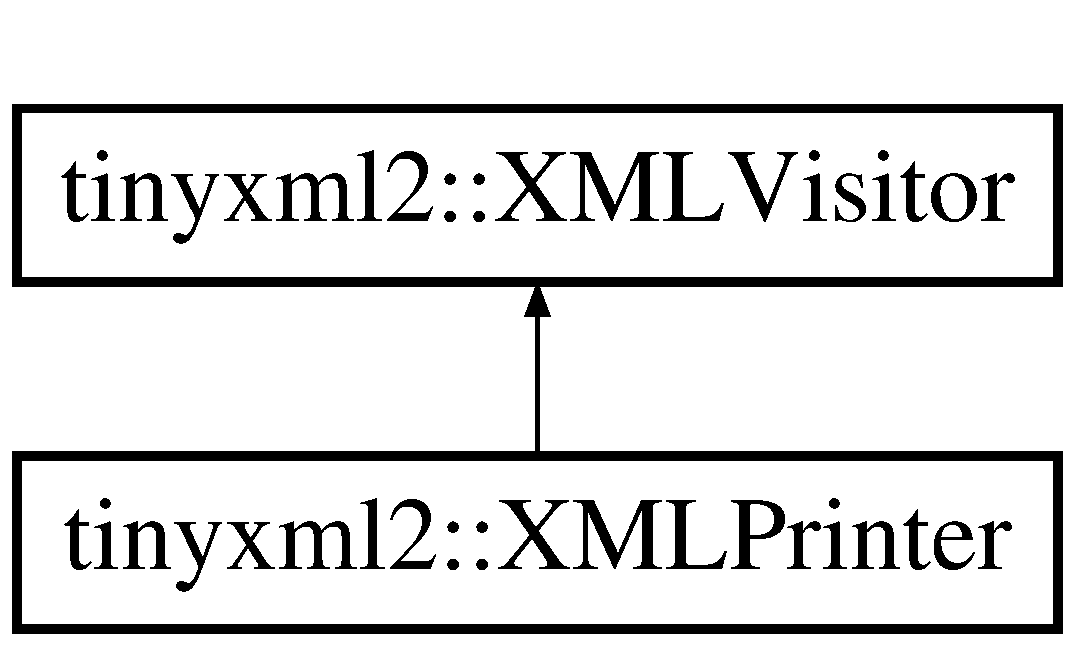
\includegraphics[height=2.000000cm]{classtinyxml2_1_1_x_m_l_visitor}
\end{center}
\end{figure}
\subsection*{Public Member Functions}
\begin{DoxyCompactItemize}
\item 
virtual \hyperlink{classtinyxml2_1_1_x_m_l_visitor_a494e72033d646c47d9c65c502ec62364}{$\sim$\-X\-M\-L\-Visitor} ()
\item 
virtual bool \hyperlink{classtinyxml2_1_1_x_m_l_visitor_acb3c22fc5f60eb9db98f533f2761f67d}{Visit\-Enter} (const \hyperlink{classtinyxml2_1_1_x_m_l_document}{X\-M\-L\-Document} \&)
\begin{DoxyCompactList}\small\item\em Visit a document. \end{DoxyCompactList}\item 
virtual bool \hyperlink{classtinyxml2_1_1_x_m_l_visitor_a170e9989cd046ba904f302d087e07086}{Visit\-Exit} (const \hyperlink{classtinyxml2_1_1_x_m_l_document}{X\-M\-L\-Document} \&)
\begin{DoxyCompactList}\small\item\em Visit a document. \end{DoxyCompactList}\item 
virtual bool \hyperlink{classtinyxml2_1_1_x_m_l_visitor_af97980a17dd4e37448b181f5ddfa92b5}{Visit\-Enter} (const \hyperlink{classtinyxml2_1_1_x_m_l_element}{X\-M\-L\-Element} \&, const \hyperlink{classtinyxml2_1_1_x_m_l_attribute}{X\-M\-L\-Attribute} $\ast$)
\begin{DoxyCompactList}\small\item\em Visit an element. \end{DoxyCompactList}\item 
virtual bool \hyperlink{classtinyxml2_1_1_x_m_l_visitor_a772f10ddc83f881956d32628faa16eb6}{Visit\-Exit} (const \hyperlink{classtinyxml2_1_1_x_m_l_element}{X\-M\-L\-Element} \&)
\begin{DoxyCompactList}\small\item\em Visit an element. \end{DoxyCompactList}\item 
virtual bool \hyperlink{classtinyxml2_1_1_x_m_l_visitor_adc75bd459fc7ba8223b50f0616767f9a}{Visit} (const \hyperlink{classtinyxml2_1_1_x_m_l_declaration}{X\-M\-L\-Declaration} \&)
\begin{DoxyCompactList}\small\item\em Visit a declaration. \end{DoxyCompactList}\item 
virtual bool \hyperlink{classtinyxml2_1_1_x_m_l_visitor_af30233565856480ea48b6fa0d6dec65b}{Visit} (const \hyperlink{classtinyxml2_1_1_x_m_l_text}{X\-M\-L\-Text} \&)
\begin{DoxyCompactList}\small\item\em Visit a text node. \end{DoxyCompactList}\item 
virtual bool \hyperlink{classtinyxml2_1_1_x_m_l_visitor_acc8147fb5a85f6c65721654e427752d7}{Visit} (const \hyperlink{classtinyxml2_1_1_x_m_l_comment}{X\-M\-L\-Comment} \&)
\begin{DoxyCompactList}\small\item\em Visit a comment node. \end{DoxyCompactList}\item 
virtual bool \hyperlink{classtinyxml2_1_1_x_m_l_visitor_a14e4748387c34bf53d24e8119bb1f292}{Visit} (const \hyperlink{classtinyxml2_1_1_x_m_l_unknown}{X\-M\-L\-Unknown} \&)
\begin{DoxyCompactList}\small\item\em Visit an unknown node. \end{DoxyCompactList}\end{DoxyCompactItemize}


\subsection{Detailed Description}
Implements the interface to the \char`\"{}\-Visitor pattern\char`\"{} (see the Accept() method.) If you call the Accept() method, it requires being passed a \hyperlink{classtinyxml2_1_1_x_m_l_visitor}{X\-M\-L\-Visitor} class to handle callbacks. For nodes that contain other nodes (Document, Element) you will get called with a Visit\-Enter/\-Visit\-Exit pair. Nodes that are always leafs are simply called with \hyperlink{classtinyxml2_1_1_x_m_l_visitor_adc75bd459fc7ba8223b50f0616767f9a}{Visit()}.

If you return 'true' from a Visit method, recursive parsing will continue. If you return false, {\bfseries no children of this node or its siblings} will be visited.

All flavors of Visit methods have a default implementation that returns 'true' (continue visiting). You need to only override methods that are interesting to you.

Generally Accept() is called on the \hyperlink{classtinyxml2_1_1_x_m_l_document}{X\-M\-L\-Document}, although all nodes support visiting.

You should never change the document from a callback.

\begin{DoxySeeAlso}{See Also}
\hyperlink{classtinyxml2_1_1_x_m_l_node_a81e66df0a44c67a7af17f3b77a152785}{X\-M\-L\-Node\-::\-Accept()} 
\end{DoxySeeAlso}


\subsection{Constructor \& Destructor Documentation}
\hypertarget{classtinyxml2_1_1_x_m_l_visitor_a494e72033d646c47d9c65c502ec62364}{\index{tinyxml2\-::\-X\-M\-L\-Visitor@{tinyxml2\-::\-X\-M\-L\-Visitor}!$\sim$\-X\-M\-L\-Visitor@{$\sim$\-X\-M\-L\-Visitor}}
\index{$\sim$\-X\-M\-L\-Visitor@{$\sim$\-X\-M\-L\-Visitor}!tinyxml2::XMLVisitor@{tinyxml2\-::\-X\-M\-L\-Visitor}}
\subsubsection[{$\sim$\-X\-M\-L\-Visitor}]{\setlength{\rightskip}{0pt plus 5cm}virtual tinyxml2\-::\-X\-M\-L\-Visitor\-::$\sim$\-X\-M\-L\-Visitor (
\begin{DoxyParamCaption}
{}
\end{DoxyParamCaption}
)\hspace{0.3cm}{\ttfamily [inline]}, {\ttfamily [virtual]}}}\label{classtinyxml2_1_1_x_m_l_visitor_a494e72033d646c47d9c65c502ec62364}


\subsection{Member Function Documentation}
\hypertarget{classtinyxml2_1_1_x_m_l_visitor_adc75bd459fc7ba8223b50f0616767f9a}{\index{tinyxml2\-::\-X\-M\-L\-Visitor@{tinyxml2\-::\-X\-M\-L\-Visitor}!Visit@{Visit}}
\index{Visit@{Visit}!tinyxml2::XMLVisitor@{tinyxml2\-::\-X\-M\-L\-Visitor}}
\subsubsection[{Visit}]{\setlength{\rightskip}{0pt plus 5cm}virtual bool tinyxml2\-::\-X\-M\-L\-Visitor\-::\-Visit (
\begin{DoxyParamCaption}
\item[{const {\bf X\-M\-L\-Declaration} \&}]{}
\end{DoxyParamCaption}
)\hspace{0.3cm}{\ttfamily [inline]}, {\ttfamily [virtual]}}}\label{classtinyxml2_1_1_x_m_l_visitor_adc75bd459fc7ba8223b50f0616767f9a}


Visit a declaration. 



Reimplemented in \hyperlink{classtinyxml2_1_1_x_m_l_printer_acfc625b2549304b9c7eb85ebd5c5eb39}{tinyxml2\-::\-X\-M\-L\-Printer}.

\hypertarget{classtinyxml2_1_1_x_m_l_visitor_af30233565856480ea48b6fa0d6dec65b}{\index{tinyxml2\-::\-X\-M\-L\-Visitor@{tinyxml2\-::\-X\-M\-L\-Visitor}!Visit@{Visit}}
\index{Visit@{Visit}!tinyxml2::XMLVisitor@{tinyxml2\-::\-X\-M\-L\-Visitor}}
\subsubsection[{Visit}]{\setlength{\rightskip}{0pt plus 5cm}virtual bool tinyxml2\-::\-X\-M\-L\-Visitor\-::\-Visit (
\begin{DoxyParamCaption}
\item[{const {\bf X\-M\-L\-Text} \&}]{}
\end{DoxyParamCaption}
)\hspace{0.3cm}{\ttfamily [inline]}, {\ttfamily [virtual]}}}\label{classtinyxml2_1_1_x_m_l_visitor_af30233565856480ea48b6fa0d6dec65b}


Visit a text node. 



Reimplemented in \hyperlink{classtinyxml2_1_1_x_m_l_printer_adc0e42b4f6fcb90a95630c79575d030b}{tinyxml2\-::\-X\-M\-L\-Printer}.

\hypertarget{classtinyxml2_1_1_x_m_l_visitor_acc8147fb5a85f6c65721654e427752d7}{\index{tinyxml2\-::\-X\-M\-L\-Visitor@{tinyxml2\-::\-X\-M\-L\-Visitor}!Visit@{Visit}}
\index{Visit@{Visit}!tinyxml2::XMLVisitor@{tinyxml2\-::\-X\-M\-L\-Visitor}}
\subsubsection[{Visit}]{\setlength{\rightskip}{0pt plus 5cm}virtual bool tinyxml2\-::\-X\-M\-L\-Visitor\-::\-Visit (
\begin{DoxyParamCaption}
\item[{const {\bf X\-M\-L\-Comment} \&}]{}
\end{DoxyParamCaption}
)\hspace{0.3cm}{\ttfamily [inline]}, {\ttfamily [virtual]}}}\label{classtinyxml2_1_1_x_m_l_visitor_acc8147fb5a85f6c65721654e427752d7}


Visit a comment node. 



Reimplemented in \hyperlink{classtinyxml2_1_1_x_m_l_printer_aa294c5c01af0ebb9114902456e4cb53c}{tinyxml2\-::\-X\-M\-L\-Printer}.

\hypertarget{classtinyxml2_1_1_x_m_l_visitor_a14e4748387c34bf53d24e8119bb1f292}{\index{tinyxml2\-::\-X\-M\-L\-Visitor@{tinyxml2\-::\-X\-M\-L\-Visitor}!Visit@{Visit}}
\index{Visit@{Visit}!tinyxml2::XMLVisitor@{tinyxml2\-::\-X\-M\-L\-Visitor}}
\subsubsection[{Visit}]{\setlength{\rightskip}{0pt plus 5cm}virtual bool tinyxml2\-::\-X\-M\-L\-Visitor\-::\-Visit (
\begin{DoxyParamCaption}
\item[{const {\bf X\-M\-L\-Unknown} \&}]{}
\end{DoxyParamCaption}
)\hspace{0.3cm}{\ttfamily [inline]}, {\ttfamily [virtual]}}}\label{classtinyxml2_1_1_x_m_l_visitor_a14e4748387c34bf53d24e8119bb1f292}


Visit an unknown node. 



Reimplemented in \hyperlink{classtinyxml2_1_1_x_m_l_printer_ab8af5455bbf9e4be2663e6642fcd7e32}{tinyxml2\-::\-X\-M\-L\-Printer}.

\hypertarget{classtinyxml2_1_1_x_m_l_visitor_acb3c22fc5f60eb9db98f533f2761f67d}{\index{tinyxml2\-::\-X\-M\-L\-Visitor@{tinyxml2\-::\-X\-M\-L\-Visitor}!Visit\-Enter@{Visit\-Enter}}
\index{Visit\-Enter@{Visit\-Enter}!tinyxml2::XMLVisitor@{tinyxml2\-::\-X\-M\-L\-Visitor}}
\subsubsection[{Visit\-Enter}]{\setlength{\rightskip}{0pt plus 5cm}virtual bool tinyxml2\-::\-X\-M\-L\-Visitor\-::\-Visit\-Enter (
\begin{DoxyParamCaption}
\item[{const {\bf X\-M\-L\-Document} \&}]{}
\end{DoxyParamCaption}
)\hspace{0.3cm}{\ttfamily [inline]}, {\ttfamily [virtual]}}}\label{classtinyxml2_1_1_x_m_l_visitor_acb3c22fc5f60eb9db98f533f2761f67d}


Visit a document. 



Reimplemented in \hyperlink{classtinyxml2_1_1_x_m_l_printer_a9aa1de11a55a07db55a90fde37d7afad}{tinyxml2\-::\-X\-M\-L\-Printer}.

\hypertarget{classtinyxml2_1_1_x_m_l_visitor_af97980a17dd4e37448b181f5ddfa92b5}{\index{tinyxml2\-::\-X\-M\-L\-Visitor@{tinyxml2\-::\-X\-M\-L\-Visitor}!Visit\-Enter@{Visit\-Enter}}
\index{Visit\-Enter@{Visit\-Enter}!tinyxml2::XMLVisitor@{tinyxml2\-::\-X\-M\-L\-Visitor}}
\subsubsection[{Visit\-Enter}]{\setlength{\rightskip}{0pt plus 5cm}virtual bool tinyxml2\-::\-X\-M\-L\-Visitor\-::\-Visit\-Enter (
\begin{DoxyParamCaption}
\item[{const {\bf X\-M\-L\-Element} \&}]{, }
\item[{const {\bf X\-M\-L\-Attribute} $\ast$}]{}
\end{DoxyParamCaption}
)\hspace{0.3cm}{\ttfamily [inline]}, {\ttfamily [virtual]}}}\label{classtinyxml2_1_1_x_m_l_visitor_af97980a17dd4e37448b181f5ddfa92b5}


Visit an element. 



Reimplemented in \hyperlink{classtinyxml2_1_1_x_m_l_printer_a169b2509d8eabb70811b2bb8cfd1f5d1}{tinyxml2\-::\-X\-M\-L\-Printer}.

\hypertarget{classtinyxml2_1_1_x_m_l_visitor_a170e9989cd046ba904f302d087e07086}{\index{tinyxml2\-::\-X\-M\-L\-Visitor@{tinyxml2\-::\-X\-M\-L\-Visitor}!Visit\-Exit@{Visit\-Exit}}
\index{Visit\-Exit@{Visit\-Exit}!tinyxml2::XMLVisitor@{tinyxml2\-::\-X\-M\-L\-Visitor}}
\subsubsection[{Visit\-Exit}]{\setlength{\rightskip}{0pt plus 5cm}virtual bool tinyxml2\-::\-X\-M\-L\-Visitor\-::\-Visit\-Exit (
\begin{DoxyParamCaption}
\item[{const {\bf X\-M\-L\-Document} \&}]{}
\end{DoxyParamCaption}
)\hspace{0.3cm}{\ttfamily [inline]}, {\ttfamily [virtual]}}}\label{classtinyxml2_1_1_x_m_l_visitor_a170e9989cd046ba904f302d087e07086}


Visit a document. 



Reimplemented in \hyperlink{classtinyxml2_1_1_x_m_l_printer_a15fc1f2b922f540917dcf52808737b29}{tinyxml2\-::\-X\-M\-L\-Printer}.

\hypertarget{classtinyxml2_1_1_x_m_l_visitor_a772f10ddc83f881956d32628faa16eb6}{\index{tinyxml2\-::\-X\-M\-L\-Visitor@{tinyxml2\-::\-X\-M\-L\-Visitor}!Visit\-Exit@{Visit\-Exit}}
\index{Visit\-Exit@{Visit\-Exit}!tinyxml2::XMLVisitor@{tinyxml2\-::\-X\-M\-L\-Visitor}}
\subsubsection[{Visit\-Exit}]{\setlength{\rightskip}{0pt plus 5cm}virtual bool tinyxml2\-::\-X\-M\-L\-Visitor\-::\-Visit\-Exit (
\begin{DoxyParamCaption}
\item[{const {\bf X\-M\-L\-Element} \&}]{}
\end{DoxyParamCaption}
)\hspace{0.3cm}{\ttfamily [inline]}, {\ttfamily [virtual]}}}\label{classtinyxml2_1_1_x_m_l_visitor_a772f10ddc83f881956d32628faa16eb6}


Visit an element. 



Reimplemented in \hyperlink{classtinyxml2_1_1_x_m_l_printer_a2edd48405971a88951c71c9df86a2f50}{tinyxml2\-::\-X\-M\-L\-Printer}.



The documentation for this class was generated from the following file\-:\begin{DoxyCompactItemize}
\item 
Joes\-\_\-\-S\-D\-L\-\_\-\-Framework/\hyperlink{tinyxml2_8h}{tinyxml2.\-h}\end{DoxyCompactItemize}

\chapter{File Documentation}
\hypertarget{_basic_maze_a_star_8h}{\section{Joes\-\_\-\-S\-D\-L\-\_\-\-Framework/\-Basic\-Maze\-A\-Star.h File Reference}
\label{_basic_maze_a_star_8h}\index{Joes\-\_\-\-S\-D\-L\-\_\-\-Framework/\-Basic\-Maze\-A\-Star.\-h@{Joes\-\_\-\-S\-D\-L\-\_\-\-Framework/\-Basic\-Maze\-A\-Star.\-h}}
}
{\ttfamily \#include \char`\"{}Scene.\-h\char`\"{}}\\*
{\ttfamily \#include $<$S\-D\-L.\-h$>$}\\*
{\ttfamily \#include \char`\"{}Tile\-Engine.\-h\char`\"{}}\\*
{\ttfamily \#include \char`\"{}X\-D\-L\-\_\-\-Path\-Finder.\-h\char`\"{}}\\*
\subsection*{Classes}
\begin{DoxyCompactItemize}
\item 
class \hyperlink{class_basic_maze_a_star}{Basic\-Maze\-A\-Star}
\end{DoxyCompactItemize}

\hypertarget{_desert_8h}{\section{Joes\-\_\-\-S\-D\-L\-\_\-\-Framework/\-Desert.h File Reference}
\label{_desert_8h}\index{Joes\-\_\-\-S\-D\-L\-\_\-\-Framework/\-Desert.\-h@{Joes\-\_\-\-S\-D\-L\-\_\-\-Framework/\-Desert.\-h}}
}
{\ttfamily \#include \char`\"{}Scene.\-h\char`\"{}}\\*
{\ttfamily \#include $<$S\-D\-L.\-h$>$}\\*
{\ttfamily \#include \char`\"{}Tile\-Engine.\-h\char`\"{}}\\*
\subsection*{Classes}
\begin{DoxyCompactItemize}
\item 
class \hyperlink{class_desert}{Desert}
\end{DoxyCompactItemize}

\hypertarget{_iso_layer_8cpp}{\section{Joes\-\_\-\-S\-D\-L\-\_\-\-Framework/\-Iso\-Layer.cpp File Reference}
\label{_iso_layer_8cpp}\index{Joes\-\_\-\-S\-D\-L\-\_\-\-Framework/\-Iso\-Layer.\-cpp@{Joes\-\_\-\-S\-D\-L\-\_\-\-Framework/\-Iso\-Layer.\-cpp}}
}
{\ttfamily \#include \char`\"{}Iso\-Layer.\-h\char`\"{}}\\*

\hypertarget{_iso_layer_8h}{\section{Joes\-\_\-\-S\-D\-L\-\_\-\-Framework/\-Iso\-Layer.h File Reference}
\label{_iso_layer_8h}\index{Joes\-\_\-\-S\-D\-L\-\_\-\-Framework/\-Iso\-Layer.\-h@{Joes\-\_\-\-S\-D\-L\-\_\-\-Framework/\-Iso\-Layer.\-h}}
}
{\ttfamily \#include $<$vector$>$}\\*
{\ttfamily \#include \char`\"{}X\-D\-L\-\_\-\-Sprite.\-h\char`\"{}}\\*
{\ttfamily \#include \char`\"{}tinyxml2.\-h\char`\"{}}\\*
\subsection*{Classes}
\begin{DoxyCompactItemize}
\item 
class \hyperlink{class_iso_layer}{Iso\-Layer}
\end{DoxyCompactItemize}

\hypertarget{_isometric_tile_engine_8cpp}{\section{Joes\-\_\-\-S\-D\-L\-\_\-\-Framework/\-Isometric\-Tile\-Engine.cpp File Reference}
\label{_isometric_tile_engine_8cpp}\index{Joes\-\_\-\-S\-D\-L\-\_\-\-Framework/\-Isometric\-Tile\-Engine.\-cpp@{Joes\-\_\-\-S\-D\-L\-\_\-\-Framework/\-Isometric\-Tile\-Engine.\-cpp}}
}
{\ttfamily \#include \char`\"{}Isometric\-Tile\-Engine.\-h\char`\"{}}\\*

\hypertarget{_isometric_tile_engine_8h}{\section{Joes\-\_\-\-S\-D\-L\-\_\-\-Framework/\-Isometric\-Tile\-Engine.h File Reference}
\label{_isometric_tile_engine_8h}\index{Joes\-\_\-\-S\-D\-L\-\_\-\-Framework/\-Isometric\-Tile\-Engine.\-h@{Joes\-\_\-\-S\-D\-L\-\_\-\-Framework/\-Isometric\-Tile\-Engine.\-h}}
}
{\ttfamily \#include $<$vector$>$}\\*
{\ttfamily \#include \char`\"{}X\-D\-L\-\_\-\-Sprite.\-h\char`\"{}}\\*
{\ttfamily \#include \char`\"{}tinyxml2.\-h\char`\"{}}\\*
{\ttfamily \#include \char`\"{}Iso\-Layer.\-h\char`\"{}}\\*
\subsection*{Classes}
\begin{DoxyCompactItemize}
\item 
class \hyperlink{class_isometric_tile_engine}{Isometric\-Tile\-Engine}
\end{DoxyCompactItemize}

\hypertarget{_level1_8cpp}{\section{Joes\-\_\-\-S\-D\-L\-\_\-\-Framework/\-Level1.cpp File Reference}
\label{_level1_8cpp}\index{Joes\-\_\-\-S\-D\-L\-\_\-\-Framework/\-Level1.\-cpp@{Joes\-\_\-\-S\-D\-L\-\_\-\-Framework/\-Level1.\-cpp}}
}
{\ttfamily \#include \char`\"{}Level1.\-h\char`\"{}}\\*
\subsection*{Variables}
\begin{DoxyCompactItemize}
\item 
\hyperlink{class_x_d_l___sprite}{X\-D\-L\-\_\-\-Sprite} $\ast$ \hyperlink{_level1_8cpp_a42cdb9591a5fc8edad0b224f0e77a1ec}{\-\_\-sprite}
\end{DoxyCompactItemize}


\subsection{Variable Documentation}
\hypertarget{_level1_8cpp_a42cdb9591a5fc8edad0b224f0e77a1ec}{\index{Level1.\-cpp@{Level1.\-cpp}!\-\_\-sprite@{\-\_\-sprite}}
\index{\-\_\-sprite@{\-\_\-sprite}!Level1.cpp@{Level1.\-cpp}}
\subsubsection[{\-\_\-sprite}]{\setlength{\rightskip}{0pt plus 5cm}{\bf X\-D\-L\-\_\-\-Sprite}$\ast$ \-\_\-sprite}}\label{_level1_8cpp_a42cdb9591a5fc8edad0b224f0e77a1ec}

\hypertarget{_level1_8h}{\section{Joes\-\_\-\-S\-D\-L\-\_\-\-Framework/\-Level1.h File Reference}
\label{_level1_8h}\index{Joes\-\_\-\-S\-D\-L\-\_\-\-Framework/\-Level1.\-h@{Joes\-\_\-\-S\-D\-L\-\_\-\-Framework/\-Level1.\-h}}
}
{\ttfamily \#include \char`\"{}X\-D\-L\-\_\-\-Scene.\-h\char`\"{}}\\*
\subsection*{Classes}
\begin{DoxyCompactItemize}
\item 
class \hyperlink{class_level1}{Level1}
\end{DoxyCompactItemize}

\hypertarget{_my_main_8h}{\section{Joes\-\_\-\-S\-D\-L\-\_\-\-Framework/\-My\-Main.h File Reference}
\label{_my_main_8h}\index{Joes\-\_\-\-S\-D\-L\-\_\-\-Framework/\-My\-Main.\-h@{Joes\-\_\-\-S\-D\-L\-\_\-\-Framework/\-My\-Main.\-h}}
}

\hypertarget{_player_8cpp}{\section{Joes\-\_\-\-S\-D\-L\-\_\-\-Framework/\-Player.cpp File Reference}
\label{_player_8cpp}\index{Joes\-\_\-\-S\-D\-L\-\_\-\-Framework/\-Player.\-cpp@{Joes\-\_\-\-S\-D\-L\-\_\-\-Framework/\-Player.\-cpp}}
}
{\ttfamily \#include \char`\"{}Player.\-h\char`\"{}}\\*
{\ttfamily \#include $<$random$>$}\\*

\hypertarget{_player_8h}{\section{Joes\-\_\-\-S\-D\-L\-\_\-\-Framework/\-Player.h File Reference}
\label{_player_8h}\index{Joes\-\_\-\-S\-D\-L\-\_\-\-Framework/\-Player.\-h@{Joes\-\_\-\-S\-D\-L\-\_\-\-Framework/\-Player.\-h}}
}
{\ttfamily \#include \char`\"{}X\-D\-L\-\_\-\-Sprite.\-h\char`\"{}}\\*
{\ttfamily \#include $<$vector$>$}\\*
{\ttfamily \#include \char`\"{}X\-D\-L\-\_\-\-Game.\-h\char`\"{}}\\*
{\ttfamily \#include \char`\"{}X\-D\-L\-\_\-\-Path\-Finder.\-h\char`\"{}}\\*
\subsection*{Classes}
\begin{DoxyCompactItemize}
\item 
class \hyperlink{class_player}{Player}
\end{DoxyCompactItemize}

\hypertarget{_pokemon_town_8h}{\section{Joes\-\_\-\-S\-D\-L\-\_\-\-Framework/\-Pokemon\-Town.h File Reference}
\label{_pokemon_town_8h}\index{Joes\-\_\-\-S\-D\-L\-\_\-\-Framework/\-Pokemon\-Town.\-h@{Joes\-\_\-\-S\-D\-L\-\_\-\-Framework/\-Pokemon\-Town.\-h}}
}
{\ttfamily \#include \char`\"{}Scene.\-h\char`\"{}}\\*
{\ttfamily \#include $<$S\-D\-L.\-h$>$}\\*
{\ttfamily \#include \char`\"{}Tile\-Engine.\-h\char`\"{}}\\*
\subsection*{Classes}
\begin{DoxyCompactItemize}
\item 
class \hyperlink{class_pokemon_town}{Pokemon\-Town}
\end{DoxyCompactItemize}

\hypertarget{_swamp_8h}{\section{Joes\-\_\-\-S\-D\-L\-\_\-\-Framework/\-Swamp.h File Reference}
\label{_swamp_8h}\index{Joes\-\_\-\-S\-D\-L\-\_\-\-Framework/\-Swamp.\-h@{Joes\-\_\-\-S\-D\-L\-\_\-\-Framework/\-Swamp.\-h}}
}
{\ttfamily \#include \char`\"{}Scene.\-h\char`\"{}}\\*
{\ttfamily \#include $<$S\-D\-L.\-h$>$}\\*
{\ttfamily \#include \char`\"{}Tile\-Engine.\-h\char`\"{}}\\*
\subsection*{Classes}
\begin{DoxyCompactItemize}
\item 
class \hyperlink{class_swamp}{Swamp}
\end{DoxyCompactItemize}

\hypertarget{tinyxml2_8cpp}{\section{Joes\-\_\-\-S\-D\-L\-\_\-\-Framework/tinyxml2.cpp File Reference}
\label{tinyxml2_8cpp}\index{Joes\-\_\-\-S\-D\-L\-\_\-\-Framework/tinyxml2.\-cpp@{Joes\-\_\-\-S\-D\-L\-\_\-\-Framework/tinyxml2.\-cpp}}
}
{\ttfamily \#include \char`\"{}tinyxml2.\-h\char`\"{}}\\*
{\ttfamily \#include $<$new$>$}\\*
{\ttfamily \#include $<$cstddef$>$}\\*
\subsection*{Classes}
\begin{DoxyCompactItemize}
\item 
struct \hyperlink{structtinyxml2_1_1_entity}{tinyxml2\-::\-Entity}
\end{DoxyCompactItemize}
\subsection*{Namespaces}
\begin{DoxyCompactItemize}
\item 
\hyperlink{namespacetinyxml2}{tinyxml2}
\end{DoxyCompactItemize}
\subsection*{Macros}
\begin{DoxyCompactItemize}
\item 
\#define \hyperlink{tinyxml2_8cpp_a4c299946dbfd4ca62902537e5a0a1a75}{D\-E\-L\-E\-T\-E\-\_\-\-N\-O\-D\-E}(node)
\item 
\#define \hyperlink{tinyxml2_8cpp_a3764bbbd1a21d84d3b5a484bb3109aec}{D\-E\-L\-E\-T\-E\-\_\-\-A\-T\-T\-R\-I\-B\-U\-T\-E}(attrib)
\end{DoxyCompactItemize}


\subsection{Macro Definition Documentation}
\hypertarget{tinyxml2_8cpp_a3764bbbd1a21d84d3b5a484bb3109aec}{\index{tinyxml2.\-cpp@{tinyxml2.\-cpp}!D\-E\-L\-E\-T\-E\-\_\-\-A\-T\-T\-R\-I\-B\-U\-T\-E@{D\-E\-L\-E\-T\-E\-\_\-\-A\-T\-T\-R\-I\-B\-U\-T\-E}}
\index{D\-E\-L\-E\-T\-E\-\_\-\-A\-T\-T\-R\-I\-B\-U\-T\-E@{D\-E\-L\-E\-T\-E\-\_\-\-A\-T\-T\-R\-I\-B\-U\-T\-E}!tinyxml2.cpp@{tinyxml2.\-cpp}}
\subsubsection[{D\-E\-L\-E\-T\-E\-\_\-\-A\-T\-T\-R\-I\-B\-U\-T\-E}]{\setlength{\rightskip}{0pt plus 5cm}\#define D\-E\-L\-E\-T\-E\-\_\-\-A\-T\-T\-R\-I\-B\-U\-T\-E(
\begin{DoxyParamCaption}
\item[{}]{attrib}
\end{DoxyParamCaption}
)}}\label{tinyxml2_8cpp_a3764bbbd1a21d84d3b5a484bb3109aec}
{\bfseries Value\-:}
\begin{DoxyCode}
\{       \(\backslash\)
        if ( attrib ) \{                         \(\backslash\)
            MemPool* pool = attrib->\_memPool;   \(\backslash\)
            attrib->~XMLAttribute();            \(\backslash\)
            pool->Free( attrib );               \(\backslash\)
        \}                                       \(\backslash\)
    \}
\end{DoxyCode}
\hypertarget{tinyxml2_8cpp_a4c299946dbfd4ca62902537e5a0a1a75}{\index{tinyxml2.\-cpp@{tinyxml2.\-cpp}!D\-E\-L\-E\-T\-E\-\_\-\-N\-O\-D\-E@{D\-E\-L\-E\-T\-E\-\_\-\-N\-O\-D\-E}}
\index{D\-E\-L\-E\-T\-E\-\_\-\-N\-O\-D\-E@{D\-E\-L\-E\-T\-E\-\_\-\-N\-O\-D\-E}!tinyxml2.cpp@{tinyxml2.\-cpp}}
\subsubsection[{D\-E\-L\-E\-T\-E\-\_\-\-N\-O\-D\-E}]{\setlength{\rightskip}{0pt plus 5cm}\#define D\-E\-L\-E\-T\-E\-\_\-\-N\-O\-D\-E(
\begin{DoxyParamCaption}
\item[{}]{node}
\end{DoxyParamCaption}
)}}\label{tinyxml2_8cpp_a4c299946dbfd4ca62902537e5a0a1a75}
{\bfseries Value\-:}
\begin{DoxyCode}
\{           \(\backslash\)
        if ( node ) \{                       \(\backslash\)
            MemPool* pool = node->\_memPool; \(\backslash\)
            node->~XMLNode();               \(\backslash\)
            pool->Free( node );             \(\backslash\)
        \}                                   \(\backslash\)
    \}
\end{DoxyCode}

\hypertarget{tinyxml2_8h}{\section{Joes\-\_\-\-S\-D\-L\-\_\-\-Framework/tinyxml2.h File Reference}
\label{tinyxml2_8h}\index{Joes\-\_\-\-S\-D\-L\-\_\-\-Framework/tinyxml2.\-h@{Joes\-\_\-\-S\-D\-L\-\_\-\-Framework/tinyxml2.\-h}}
}
{\ttfamily \#include $<$cctype$>$}\\*
{\ttfamily \#include $<$climits$>$}\\*
{\ttfamily \#include $<$cstdio$>$}\\*
{\ttfamily \#include $<$cstdlib$>$}\\*
{\ttfamily \#include $<$cstring$>$}\\*
{\ttfamily \#include $<$cstdarg$>$}\\*
\subsection*{Classes}
\begin{DoxyCompactItemize}
\item 
class \hyperlink{classtinyxml2_1_1_str_pair}{tinyxml2\-::\-Str\-Pair}
\item 
class \hyperlink{classtinyxml2_1_1_dyn_array}{tinyxml2\-::\-Dyn\-Array$<$ T, I\-N\-I\-T $>$}
\item 
class \hyperlink{classtinyxml2_1_1_mem_pool}{tinyxml2\-::\-Mem\-Pool}
\item 
class \hyperlink{classtinyxml2_1_1_mem_pool_t}{tinyxml2\-::\-Mem\-Pool\-T$<$ S\-I\-Z\-E $>$}
\item 
class \hyperlink{classtinyxml2_1_1_x_m_l_visitor}{tinyxml2\-::\-X\-M\-L\-Visitor}
\item 
class \hyperlink{classtinyxml2_1_1_x_m_l_util}{tinyxml2\-::\-X\-M\-L\-Util}
\item 
class \hyperlink{classtinyxml2_1_1_x_m_l_node}{tinyxml2\-::\-X\-M\-L\-Node}
\item 
class \hyperlink{classtinyxml2_1_1_x_m_l_text}{tinyxml2\-::\-X\-M\-L\-Text}
\item 
class \hyperlink{classtinyxml2_1_1_x_m_l_comment}{tinyxml2\-::\-X\-M\-L\-Comment}
\item 
class \hyperlink{classtinyxml2_1_1_x_m_l_declaration}{tinyxml2\-::\-X\-M\-L\-Declaration}
\item 
class \hyperlink{classtinyxml2_1_1_x_m_l_unknown}{tinyxml2\-::\-X\-M\-L\-Unknown}
\item 
class \hyperlink{classtinyxml2_1_1_x_m_l_attribute}{tinyxml2\-::\-X\-M\-L\-Attribute}
\item 
class \hyperlink{classtinyxml2_1_1_x_m_l_element}{tinyxml2\-::\-X\-M\-L\-Element}
\item 
class \hyperlink{classtinyxml2_1_1_x_m_l_document}{tinyxml2\-::\-X\-M\-L\-Document}
\item 
class \hyperlink{classtinyxml2_1_1_x_m_l_handle}{tinyxml2\-::\-X\-M\-L\-Handle}
\item 
class \hyperlink{classtinyxml2_1_1_x_m_l_const_handle}{tinyxml2\-::\-X\-M\-L\-Const\-Handle}
\item 
class \hyperlink{classtinyxml2_1_1_x_m_l_printer}{tinyxml2\-::\-X\-M\-L\-Printer}
\end{DoxyCompactItemize}
\subsection*{Namespaces}
\begin{DoxyCompactItemize}
\item 
\hyperlink{namespacetinyxml2}{tinyxml2}
\end{DoxyCompactItemize}
\subsection*{Macros}
\begin{DoxyCompactItemize}
\item 
\#define \hyperlink{tinyxml2_8h_a8953517b8490d756ad0bfef40fe5811f}{T\-I\-N\-Y\-X\-M\-L2\-\_\-\-L\-I\-B}
\item 
\#define \hyperlink{tinyxml2_8h_a029877acb3c6fd71698561044953bd14}{T\-I\-X\-M\-L\-A\-S\-S\-E\-R\-T}(x)~\{\}
\item 
\#define \hyperlink{tinyxml2_8h_afc6433f9b56e4f18833089b1df629e0a}{T\-I\-X\-M\-L\-\_\-\-S\-N\-P\-R\-I\-N\-T\-F}~snprintf
\item 
\#define \hyperlink{tinyxml2_8h_a96f54d7c855ad92e705510904a040393}{T\-I\-X\-M\-L\-\_\-\-S\-S\-C\-A\-N\-F}~sscanf
\end{DoxyCompactItemize}
\subsection*{Enumerations}
\begin{DoxyCompactItemize}
\item 
enum \hyperlink{namespacetinyxml2_a1fbf88509c3ac88c09117b1947414e08}{tinyxml2\-::\-X\-M\-L\-Error} \{ \\*
\hyperlink{namespacetinyxml2_a1fbf88509c3ac88c09117b1947414e08ad3b3f200ced09c9fc4166134a4ff8fef}{tinyxml2\-::\-X\-M\-L\-\_\-\-N\-O\-\_\-\-E\-R\-R\-O\-R} = 0, 
\hyperlink{namespacetinyxml2_a1fbf88509c3ac88c09117b1947414e08a1fe1262fdb5ac05dd9cc4631f8c8e00d}{tinyxml2\-::\-X\-M\-L\-\_\-\-S\-U\-C\-C\-E\-S\-S} = 0, 
\hyperlink{namespacetinyxml2_a1fbf88509c3ac88c09117b1947414e08abefb89c44285fb68e2218b2c71767f27}{tinyxml2\-::\-X\-M\-L\-\_\-\-N\-O\-\_\-\-A\-T\-T\-R\-I\-B\-U\-T\-E}, 
\hyperlink{namespacetinyxml2_a1fbf88509c3ac88c09117b1947414e08ae9d8ee545a3a69e90df303257a658113}{tinyxml2\-::\-X\-M\-L\-\_\-\-W\-R\-O\-N\-G\-\_\-\-A\-T\-T\-R\-I\-B\-U\-T\-E\-\_\-\-T\-Y\-P\-E}, 
\\*
\hyperlink{namespacetinyxml2_a1fbf88509c3ac88c09117b1947414e08a38fd2a97fb1dbebd4c3640d75dc01a94}{tinyxml2\-::\-X\-M\-L\-\_\-\-E\-R\-R\-O\-R\-\_\-\-F\-I\-L\-E\-\_\-\-N\-O\-T\-\_\-\-F\-O\-U\-N\-D}, 
\hyperlink{namespacetinyxml2_a1fbf88509c3ac88c09117b1947414e08afbbf37655523b79a88b04b77ec0f1258}{tinyxml2\-::\-X\-M\-L\-\_\-\-E\-R\-R\-O\-R\-\_\-\-F\-I\-L\-E\-\_\-\-C\-O\-U\-L\-D\-\_\-\-N\-O\-T\-\_\-\-B\-E\-\_\-\-O\-P\-E\-N\-E\-D}, 
\hyperlink{namespacetinyxml2_a1fbf88509c3ac88c09117b1947414e08a8d4dd3ce2dee784a53f62fa8a6ac83ee}{tinyxml2\-::\-X\-M\-L\-\_\-\-E\-R\-R\-O\-R\-\_\-\-F\-I\-L\-E\-\_\-\-R\-E\-A\-D\-\_\-\-E\-R\-R\-O\-R}, 
\hyperlink{namespacetinyxml2_a1fbf88509c3ac88c09117b1947414e08a37759723c0c5e954597654e4eccb4f4d}{tinyxml2\-::\-X\-M\-L\-\_\-\-E\-R\-R\-O\-R\-\_\-\-E\-L\-E\-M\-E\-N\-T\-\_\-\-M\-I\-S\-M\-A\-T\-C\-H}, 
\\*
\hyperlink{namespacetinyxml2_a1fbf88509c3ac88c09117b1947414e08afa96ea783aa93ea212f9e2d7d3a70ba5}{tinyxml2\-::\-X\-M\-L\-\_\-\-E\-R\-R\-O\-R\-\_\-\-P\-A\-R\-S\-I\-N\-G\-\_\-\-E\-L\-E\-M\-E\-N\-T}, 
\hyperlink{namespacetinyxml2_a1fbf88509c3ac88c09117b1947414e08a380fd8846799b88773321efae83d26a3}{tinyxml2\-::\-X\-M\-L\-\_\-\-E\-R\-R\-O\-R\-\_\-\-P\-A\-R\-S\-I\-N\-G\-\_\-\-A\-T\-T\-R\-I\-B\-U\-T\-E}, 
\hyperlink{namespacetinyxml2_a1fbf88509c3ac88c09117b1947414e08a48e646cfca6de90c3770faf535d3ed6b}{tinyxml2\-::\-X\-M\-L\-\_\-\-E\-R\-R\-O\-R\-\_\-\-I\-D\-E\-N\-T\-I\-F\-Y\-I\-N\-G\-\_\-\-T\-A\-G}, 
\hyperlink{namespacetinyxml2_a1fbf88509c3ac88c09117b1947414e08a50ead30b94c7ae2957b9ccb08ec0994d}{tinyxml2\-::\-X\-M\-L\-\_\-\-E\-R\-R\-O\-R\-\_\-\-P\-A\-R\-S\-I\-N\-G\-\_\-\-T\-E\-X\-T}, 
\\*
\hyperlink{namespacetinyxml2_a1fbf88509c3ac88c09117b1947414e08a9d181628a1819f2b97835e6bc2c8bb3b}{tinyxml2\-::\-X\-M\-L\-\_\-\-E\-R\-R\-O\-R\-\_\-\-P\-A\-R\-S\-I\-N\-G\-\_\-\-C\-D\-A\-T\-A}, 
\hyperlink{namespacetinyxml2_a1fbf88509c3ac88c09117b1947414e08a51786809e8b079c770853cf5890a7a35}{tinyxml2\-::\-X\-M\-L\-\_\-\-E\-R\-R\-O\-R\-\_\-\-P\-A\-R\-S\-I\-N\-G\-\_\-\-C\-O\-M\-M\-E\-N\-T}, 
\hyperlink{namespacetinyxml2_a1fbf88509c3ac88c09117b1947414e08ad45b208578e30dab5a21bff1d8991b87}{tinyxml2\-::\-X\-M\-L\-\_\-\-E\-R\-R\-O\-R\-\_\-\-P\-A\-R\-S\-I\-N\-G\-\_\-\-D\-E\-C\-L\-A\-R\-A\-T\-I\-O\-N}, 
\hyperlink{namespacetinyxml2_a1fbf88509c3ac88c09117b1947414e08a95a88813812a680fb7372f0149420a97}{tinyxml2\-::\-X\-M\-L\-\_\-\-E\-R\-R\-O\-R\-\_\-\-P\-A\-R\-S\-I\-N\-G\-\_\-\-U\-N\-K\-N\-O\-W\-N}, 
\\*
\hyperlink{namespacetinyxml2_a1fbf88509c3ac88c09117b1947414e08a1a0478cf44f0a733aa6f21bdf0db80b5}{tinyxml2\-::\-X\-M\-L\-\_\-\-E\-R\-R\-O\-R\-\_\-\-E\-M\-P\-T\-Y\-\_\-\-D\-O\-C\-U\-M\-E\-N\-T}, 
\hyperlink{namespacetinyxml2_a1fbf88509c3ac88c09117b1947414e08a0cecc816939d9155d33b8a88fd50e4c1}{tinyxml2\-::\-X\-M\-L\-\_\-\-E\-R\-R\-O\-R\-\_\-\-M\-I\-S\-M\-A\-T\-C\-H\-E\-D\-\_\-\-E\-L\-E\-M\-E\-N\-T}, 
\hyperlink{namespacetinyxml2_a1fbf88509c3ac88c09117b1947414e08af6b4caa10e1f2e9f19a3a24f5f3ce223}{tinyxml2\-::\-X\-M\-L\-\_\-\-E\-R\-R\-O\-R\-\_\-\-P\-A\-R\-S\-I\-N\-G}, 
\hyperlink{namespacetinyxml2_a1fbf88509c3ac88c09117b1947414e08afdb8840395a7c13dfe6a3e104401c095}{tinyxml2\-::\-X\-M\-L\-\_\-\-C\-A\-N\-\_\-\-N\-O\-T\-\_\-\-C\-O\-N\-V\-E\-R\-T\-\_\-\-T\-E\-X\-T}, 
\\*
\hyperlink{namespacetinyxml2_a1fbf88509c3ac88c09117b1947414e08a5300bec98feccc8f0cdf567b88821f33}{tinyxml2\-::\-X\-M\-L\-\_\-\-N\-O\-\_\-\-T\-E\-X\-T\-\_\-\-N\-O\-D\-E}
 \}
\item 
enum \hyperlink{namespacetinyxml2_a7f91d00f77360f850fd5da0861e27dd5}{tinyxml2\-::\-Whitespace} \{ \hyperlink{namespacetinyxml2_a7f91d00f77360f850fd5da0861e27dd5a751769aa625fe5fe5286e9779edec56a}{tinyxml2\-::\-P\-R\-E\-S\-E\-R\-V\-E\-\_\-\-W\-H\-I\-T\-E\-S\-P\-A\-C\-E}, 
\hyperlink{namespacetinyxml2_a7f91d00f77360f850fd5da0861e27dd5a9a4a309029a6f5e636e20ef5e0b65136}{tinyxml2\-::\-C\-O\-L\-L\-A\-P\-S\-E\-\_\-\-W\-H\-I\-T\-E\-S\-P\-A\-C\-E}
 \}
\end{DoxyCompactItemize}


\subsection{Macro Definition Documentation}
\hypertarget{tinyxml2_8h_a8953517b8490d756ad0bfef40fe5811f}{\index{tinyxml2.\-h@{tinyxml2.\-h}!T\-I\-N\-Y\-X\-M\-L2\-\_\-\-L\-I\-B@{T\-I\-N\-Y\-X\-M\-L2\-\_\-\-L\-I\-B}}
\index{T\-I\-N\-Y\-X\-M\-L2\-\_\-\-L\-I\-B@{T\-I\-N\-Y\-X\-M\-L2\-\_\-\-L\-I\-B}!tinyxml2.h@{tinyxml2.\-h}}
\subsubsection[{T\-I\-N\-Y\-X\-M\-L2\-\_\-\-L\-I\-B}]{\setlength{\rightskip}{0pt plus 5cm}\#define T\-I\-N\-Y\-X\-M\-L2\-\_\-\-L\-I\-B}}\label{tinyxml2_8h_a8953517b8490d756ad0bfef40fe5811f}
\hypertarget{tinyxml2_8h_afc6433f9b56e4f18833089b1df629e0a}{\index{tinyxml2.\-h@{tinyxml2.\-h}!T\-I\-X\-M\-L\-\_\-\-S\-N\-P\-R\-I\-N\-T\-F@{T\-I\-X\-M\-L\-\_\-\-S\-N\-P\-R\-I\-N\-T\-F}}
\index{T\-I\-X\-M\-L\-\_\-\-S\-N\-P\-R\-I\-N\-T\-F@{T\-I\-X\-M\-L\-\_\-\-S\-N\-P\-R\-I\-N\-T\-F}!tinyxml2.h@{tinyxml2.\-h}}
\subsubsection[{T\-I\-X\-M\-L\-\_\-\-S\-N\-P\-R\-I\-N\-T\-F}]{\setlength{\rightskip}{0pt plus 5cm}\#define T\-I\-X\-M\-L\-\_\-\-S\-N\-P\-R\-I\-N\-T\-F~snprintf}}\label{tinyxml2_8h_afc6433f9b56e4f18833089b1df629e0a}
\hypertarget{tinyxml2_8h_a96f54d7c855ad92e705510904a040393}{\index{tinyxml2.\-h@{tinyxml2.\-h}!T\-I\-X\-M\-L\-\_\-\-S\-S\-C\-A\-N\-F@{T\-I\-X\-M\-L\-\_\-\-S\-S\-C\-A\-N\-F}}
\index{T\-I\-X\-M\-L\-\_\-\-S\-S\-C\-A\-N\-F@{T\-I\-X\-M\-L\-\_\-\-S\-S\-C\-A\-N\-F}!tinyxml2.h@{tinyxml2.\-h}}
\subsubsection[{T\-I\-X\-M\-L\-\_\-\-S\-S\-C\-A\-N\-F}]{\setlength{\rightskip}{0pt plus 5cm}\#define T\-I\-X\-M\-L\-\_\-\-S\-S\-C\-A\-N\-F~sscanf}}\label{tinyxml2_8h_a96f54d7c855ad92e705510904a040393}
\hypertarget{tinyxml2_8h_a029877acb3c6fd71698561044953bd14}{\index{tinyxml2.\-h@{tinyxml2.\-h}!T\-I\-X\-M\-L\-A\-S\-S\-E\-R\-T@{T\-I\-X\-M\-L\-A\-S\-S\-E\-R\-T}}
\index{T\-I\-X\-M\-L\-A\-S\-S\-E\-R\-T@{T\-I\-X\-M\-L\-A\-S\-S\-E\-R\-T}!tinyxml2.h@{tinyxml2.\-h}}
\subsubsection[{T\-I\-X\-M\-L\-A\-S\-S\-E\-R\-T}]{\setlength{\rightskip}{0pt plus 5cm}\#define T\-I\-X\-M\-L\-A\-S\-S\-E\-R\-T(
\begin{DoxyParamCaption}
\item[{}]{x}
\end{DoxyParamCaption}
)~\{\}}}\label{tinyxml2_8h_a029877acb3c6fd71698561044953bd14}

\hypertarget{_variable_terrain_8h}{\section{Joes\-\_\-\-S\-D\-L\-\_\-\-Framework/\-Variable\-Terrain.h File Reference}
\label{_variable_terrain_8h}\index{Joes\-\_\-\-S\-D\-L\-\_\-\-Framework/\-Variable\-Terrain.\-h@{Joes\-\_\-\-S\-D\-L\-\_\-\-Framework/\-Variable\-Terrain.\-h}}
}
{\ttfamily \#include \char`\"{}Scene.\-h\char`\"{}}\\*
{\ttfamily \#include $<$S\-D\-L.\-h$>$}\\*
{\ttfamily \#include \char`\"{}Tile\-Engine.\-h\char`\"{}}\\*
{\ttfamily \#include \char`\"{}X\-D\-L\-\_\-\-Path\-Finder.\-h\char`\"{}}\\*
\subsection*{Classes}
\begin{DoxyCompactItemize}
\item 
class \hyperlink{class_variable_terrain}{Variable\-Terrain}
\end{DoxyCompactItemize}

\hypertarget{_x_d_l___camera_8cpp}{\section{Joes\-\_\-\-S\-D\-L\-\_\-\-Framework/\-X\-D\-L\-\_\-\-Camera.cpp File Reference}
\label{_x_d_l___camera_8cpp}\index{Joes\-\_\-\-S\-D\-L\-\_\-\-Framework/\-X\-D\-L\-\_\-\-Camera.\-cpp@{Joes\-\_\-\-S\-D\-L\-\_\-\-Framework/\-X\-D\-L\-\_\-\-Camera.\-cpp}}
}
{\ttfamily \#include \char`\"{}X\-D\-L\-\_\-\-Camera.\-h\char`\"{}}\\*

\hypertarget{_x_d_l___camera_8h}{\section{Joes\-\_\-\-S\-D\-L\-\_\-\-Framework/\-X\-D\-L\-\_\-\-Camera.h File Reference}
\label{_x_d_l___camera_8h}\index{Joes\-\_\-\-S\-D\-L\-\_\-\-Framework/\-X\-D\-L\-\_\-\-Camera.\-h@{Joes\-\_\-\-S\-D\-L\-\_\-\-Framework/\-X\-D\-L\-\_\-\-Camera.\-h}}
}
{\ttfamily \#include $<$S\-D\-L.\-h$>$}\\*
\subsection*{Classes}
\begin{DoxyCompactItemize}
\item 
class \hyperlink{class_x_d_l___camera}{X\-D\-L\-\_\-\-Camera}
\begin{DoxyCompactList}\small\item\em X\-D\-L\-\_\-\-Camaera. \mbox{[}Singleton\mbox{]}. \end{DoxyCompactList}\end{DoxyCompactItemize}

\hypertarget{_x_d_l___content_manager_8cpp}{\section{Joes\-\_\-\-S\-D\-L\-\_\-\-Framework/\-X\-D\-L\-\_\-\-Content\-Manager.cpp File Reference}
\label{_x_d_l___content_manager_8cpp}\index{Joes\-\_\-\-S\-D\-L\-\_\-\-Framework/\-X\-D\-L\-\_\-\-Content\-Manager.\-cpp@{Joes\-\_\-\-S\-D\-L\-\_\-\-Framework/\-X\-D\-L\-\_\-\-Content\-Manager.\-cpp}}
}
{\ttfamily \#include \char`\"{}X\-D\-L\-\_\-\-Content\-Manager.\-h\char`\"{}}\\*

\hypertarget{_x_d_l___content_manager_8h}{\section{Joes\-\_\-\-S\-D\-L\-\_\-\-Framework/\-X\-D\-L\-\_\-\-Content\-Manager.h File Reference}
\label{_x_d_l___content_manager_8h}\index{Joes\-\_\-\-S\-D\-L\-\_\-\-Framework/\-X\-D\-L\-\_\-\-Content\-Manager.\-h@{Joes\-\_\-\-S\-D\-L\-\_\-\-Framework/\-X\-D\-L\-\_\-\-Content\-Manager.\-h}}
}
{\ttfamily \#include $<$S\-D\-L.\-h$>$}\\*
{\ttfamily \#include $<$stdlib.\-h$>$}\\*
{\ttfamily \#include $<$iostream$>$}\\*
{\ttfamily \#include $<$map$>$}\\*
{\ttfamily \#include $<$S\-D\-L\-\_\-image.\-h$>$}\\*
\subsection*{Classes}
\begin{DoxyCompactItemize}
\item 
class \hyperlink{class_x_d_l___content_manager}{X\-D\-L\-\_\-\-Content\-Manager}
\end{DoxyCompactItemize}

\hypertarget{_x_d_l___debug_8h}{\section{Joes\-\_\-\-S\-D\-L\-\_\-\-Framework/\-X\-D\-L\-\_\-\-Debug.h File Reference}
\label{_x_d_l___debug_8h}\index{Joes\-\_\-\-S\-D\-L\-\_\-\-Framework/\-X\-D\-L\-\_\-\-Debug.\-h@{Joes\-\_\-\-S\-D\-L\-\_\-\-Framework/\-X\-D\-L\-\_\-\-Debug.\-h}}
}
\subsection*{Macros}
\begin{DoxyCompactItemize}
\item 
\#define \hyperlink{_x_d_l___debug_8h_aa46006d6606f3f94029fff98cc0ba94a}{D\-E\-B\-U\-G\-\_\-\-M\-S\-G}(x)
\begin{DoxyCompactList}\small\item\em X\-D\-L\-\_\-\-Debug. \end{DoxyCompactList}\end{DoxyCompactItemize}


\subsection{Macro Definition Documentation}
\hypertarget{_x_d_l___debug_8h_aa46006d6606f3f94029fff98cc0ba94a}{\index{X\-D\-L\-\_\-\-Debug.\-h@{X\-D\-L\-\_\-\-Debug.\-h}!D\-E\-B\-U\-G\-\_\-\-M\-S\-G@{D\-E\-B\-U\-G\-\_\-\-M\-S\-G}}
\index{D\-E\-B\-U\-G\-\_\-\-M\-S\-G@{D\-E\-B\-U\-G\-\_\-\-M\-S\-G}!XDL_Debug.h@{X\-D\-L\-\_\-\-Debug.\-h}}
\subsubsection[{D\-E\-B\-U\-G\-\_\-\-M\-S\-G}]{\setlength{\rightskip}{0pt plus 5cm}\#define D\-E\-B\-U\-G\-\_\-\-M\-S\-G(
\begin{DoxyParamCaption}
\item[{}]{x}
\end{DoxyParamCaption}
)}}\label{_x_d_l___debug_8h_aa46006d6606f3f94029fff98cc0ba94a}


X\-D\-L\-\_\-\-Debug. 

Wraps Cout, so you dont have to use C\-O\-U\-T in your code, you can use D\-E\-B\-U\-G\-\_\-\-M\-S\-G. turning D\-E\-B\-U\-G to 0 turns off all D\-E\-B\-U\-G\-\_\-\-M\-S\-G outputs 
\hypertarget{_x_d_l___game_8cpp}{\section{Joes\-\_\-\-S\-D\-L\-\_\-\-Framework/\-X\-D\-L\-\_\-\-Game.cpp File Reference}
\label{_x_d_l___game_8cpp}\index{Joes\-\_\-\-S\-D\-L\-\_\-\-Framework/\-X\-D\-L\-\_\-\-Game.\-cpp@{Joes\-\_\-\-S\-D\-L\-\_\-\-Framework/\-X\-D\-L\-\_\-\-Game.\-cpp}}
}
{\ttfamily \#include \char`\"{}X\-D\-L\-\_\-\-Game.\-h\char`\"{}}\\*
{\ttfamily \#include \char`\"{}X\-D\-L\-\_\-\-Debug.\-h\char`\"{}}\\*
{\ttfamily \#include \char`\"{}X\-D\-L\-\_\-\-Scene\-Manager.\-h\char`\"{}}\\*
{\ttfamily \#include \char`\"{}Level1.\-h\char`\"{}}\\*
\subsection*{Variables}
\begin{DoxyCompactItemize}
\item 
\hyperlink{class_x_d_l___scene_manager}{X\-D\-L\-\_\-\-Scene\-Manager} $\ast$ \hyperlink{_x_d_l___game_8cpp_af8c6274ceb43fd2a24432d333732d72f}{\-\_\-scene\-Manager}
\end{DoxyCompactItemize}


\subsection{Variable Documentation}
\hypertarget{_x_d_l___game_8cpp_af8c6274ceb43fd2a24432d333732d72f}{\index{X\-D\-L\-\_\-\-Game.\-cpp@{X\-D\-L\-\_\-\-Game.\-cpp}!\-\_\-scene\-Manager@{\-\_\-scene\-Manager}}
\index{\-\_\-scene\-Manager@{\-\_\-scene\-Manager}!XDL_Game.cpp@{X\-D\-L\-\_\-\-Game.\-cpp}}
\subsubsection[{\-\_\-scene\-Manager}]{\setlength{\rightskip}{0pt plus 5cm}{\bf X\-D\-L\-\_\-\-Scene\-Manager}$\ast$ \-\_\-scene\-Manager}}\label{_x_d_l___game_8cpp_af8c6274ceb43fd2a24432d333732d72f}

\hypertarget{_x_d_l___game_8h}{\section{Joes\-\_\-\-S\-D\-L\-\_\-\-Framework/\-X\-D\-L\-\_\-\-Game.h File Reference}
\label{_x_d_l___game_8h}\index{Joes\-\_\-\-S\-D\-L\-\_\-\-Framework/\-X\-D\-L\-\_\-\-Game.\-h@{Joes\-\_\-\-S\-D\-L\-\_\-\-Framework/\-X\-D\-L\-\_\-\-Game.\-h}}
}
{\ttfamily \#include \char`\"{}X\-D\-L\-\_\-\-Debug.\-h\char`\"{}}\\*
{\ttfamily \#include $<$S\-D\-L.\-h$>$}\\*
\subsection*{Classes}
\begin{DoxyCompactItemize}
\item 
class \hyperlink{class_x_d_l___game}{X\-D\-L\-\_\-\-Game}
\begin{DoxyCompactList}\small\item\em \hyperlink{class_x_d_l___game}{X\-D\-L\-\_\-\-Game}. \end{DoxyCompactList}\end{DoxyCompactItemize}

\hypertarget{_x_d_l___game_object_8cpp}{\section{Joes\-\_\-\-S\-D\-L\-\_\-\-Framework/\-X\-D\-L\-\_\-\-Game\-Object.cpp File Reference}
\label{_x_d_l___game_object_8cpp}\index{Joes\-\_\-\-S\-D\-L\-\_\-\-Framework/\-X\-D\-L\-\_\-\-Game\-Object.\-cpp@{Joes\-\_\-\-S\-D\-L\-\_\-\-Framework/\-X\-D\-L\-\_\-\-Game\-Object.\-cpp}}
}
{\ttfamily \#include \char`\"{}X\-D\-L\-\_\-\-Game\-Object.\-h\char`\"{}}\\*

\hypertarget{_x_d_l___game_object_8h}{\section{Joes\-\_\-\-S\-D\-L\-\_\-\-Framework/\-X\-D\-L\-\_\-\-Game\-Object.h File Reference}
\label{_x_d_l___game_object_8h}\index{Joes\-\_\-\-S\-D\-L\-\_\-\-Framework/\-X\-D\-L\-\_\-\-Game\-Object.\-h@{Joes\-\_\-\-S\-D\-L\-\_\-\-Framework/\-X\-D\-L\-\_\-\-Game\-Object.\-h}}
}
{\ttfamily \#include $<$S\-D\-L.\-h$>$}\\*
{\ttfamily \#include \char`\"{}X\-D\-L\-\_\-\-Debug.\-h\char`\"{}}\\*
\subsection*{Classes}
\begin{DoxyCompactItemize}
\item 
class \hyperlink{class_x_d_l___game_object}{X\-D\-L\-\_\-\-Game\-Object}
\begin{DoxyCompactList}\small\item\em \hyperlink{class_x_d_l___game_object}{X\-D\-L\-\_\-\-Game\-Object}. \end{DoxyCompactList}\end{DoxyCompactItemize}

\hypertarget{_x_d_l___keyboard_8cpp}{\section{Joes\-\_\-\-S\-D\-L\-\_\-\-Framework/\-X\-D\-L\-\_\-\-Keyboard.cpp File Reference}
\label{_x_d_l___keyboard_8cpp}\index{Joes\-\_\-\-S\-D\-L\-\_\-\-Framework/\-X\-D\-L\-\_\-\-Keyboard.\-cpp@{Joes\-\_\-\-S\-D\-L\-\_\-\-Framework/\-X\-D\-L\-\_\-\-Keyboard.\-cpp}}
}
{\ttfamily \#include \char`\"{}X\-D\-L\-\_\-\-Keyboard.\-h\char`\"{}}\\*

\hypertarget{_x_d_l___keyboard_8h}{\section{Joes\-\_\-\-S\-D\-L\-\_\-\-Framework/\-X\-D\-L\-\_\-\-Keyboard.h File Reference}
\label{_x_d_l___keyboard_8h}\index{Joes\-\_\-\-S\-D\-L\-\_\-\-Framework/\-X\-D\-L\-\_\-\-Keyboard.\-h@{Joes\-\_\-\-S\-D\-L\-\_\-\-Framework/\-X\-D\-L\-\_\-\-Keyboard.\-h}}
}
{\ttfamily \#include $<$S\-D\-L.\-h$>$}\\*
\subsection*{Classes}
\begin{DoxyCompactItemize}
\item 
class \hyperlink{class_x_d_l___keyboard}{X\-D\-L\-\_\-\-Keyboard}
\begin{DoxyCompactList}\small\item\em \hyperlink{class_x_d_l___keyboard}{X\-D\-L\-\_\-\-Keyboard}. \mbox{[}Singleton\mbox{]}. \end{DoxyCompactList}\end{DoxyCompactItemize}

\hypertarget{_x_d_l___layer_8cpp}{\section{Joes\-\_\-\-S\-D\-L\-\_\-\-Framework/\-X\-D\-L\-\_\-\-Layer.cpp File Reference}
\label{_x_d_l___layer_8cpp}\index{Joes\-\_\-\-S\-D\-L\-\_\-\-Framework/\-X\-D\-L\-\_\-\-Layer.\-cpp@{Joes\-\_\-\-S\-D\-L\-\_\-\-Framework/\-X\-D\-L\-\_\-\-Layer.\-cpp}}
}
{\ttfamily \#include \char`\"{}X\-D\-L\-\_\-\-Layer.\-h\char`\"{}}\\*
{\ttfamily \#include \char`\"{}X\-D\-L\-\_\-\-Sprite\-Batch.\-h\char`\"{}}\\*

\hypertarget{_x_d_l___layer_8h}{\section{Joes\-\_\-\-S\-D\-L\-\_\-\-Framework/\-X\-D\-L\-\_\-\-Layer.h File Reference}
\label{_x_d_l___layer_8h}\index{Joes\-\_\-\-S\-D\-L\-\_\-\-Framework/\-X\-D\-L\-\_\-\-Layer.\-h@{Joes\-\_\-\-S\-D\-L\-\_\-\-Framework/\-X\-D\-L\-\_\-\-Layer.\-h}}
}
{\ttfamily \#include $<$vector$>$}\\*
{\ttfamily \#include \char`\"{}X\-D\-L\-\_\-\-Tile.\-h\char`\"{}}\\*
{\ttfamily \#include \char`\"{}tinyxml2.\-h\char`\"{}}\\*
{\ttfamily \#include \char`\"{}X\-D\-L\-\_\-\-Sprite\-Batch.\-h\char`\"{}}\\*
\subsection*{Classes}
\begin{DoxyCompactItemize}
\item 
class \hyperlink{class_x_d_l___layer}{X\-D\-L\-\_\-\-Layer}
\end{DoxyCompactItemize}

\hypertarget{_x_d_l___main_8cpp}{\section{Joes\-\_\-\-S\-D\-L\-\_\-\-Framework/\-X\-D\-L\-\_\-\-Main.cpp File Reference}
\label{_x_d_l___main_8cpp}\index{Joes\-\_\-\-S\-D\-L\-\_\-\-Framework/\-X\-D\-L\-\_\-\-Main.\-cpp@{Joes\-\_\-\-S\-D\-L\-\_\-\-Framework/\-X\-D\-L\-\_\-\-Main.\-cpp}}
}
{\ttfamily \#include $<$stdlib.\-h$>$}\\*
{\ttfamily \#include \char`\"{}X\-D\-L\-\_\-\-Game.\-h\char`\"{}}\\*
{\ttfamily \#include \char`\"{}X\-D\-L\-\_\-\-Debug.\-h\char`\"{}}\\*
{\ttfamily \#include $<$chrono$>$}\\*
{\ttfamily \#include $<$thread$>$}\\*
\subsection*{Functions}
\begin{DoxyCompactItemize}
\item 
int \hyperlink{_x_d_l___main_8cpp_a700a0caa5b70a06d1064e576f9f3cf65}{main} (int argc, char $\ast$args\mbox{[}$\,$\mbox{]})
\end{DoxyCompactItemize}
\subsection*{Variables}
\begin{DoxyCompactItemize}
\item 
\hyperlink{class_x_d_l___game}{X\-D\-L\-\_\-\-Game} $\ast$ \hyperlink{_x_d_l___main_8cpp_aed86116a23347ce9907e7d8bed245578}{\-\_\-game}
\begin{DoxyCompactList}\small\item\em X\-D\-L\-\_\-\-Main. \end{DoxyCompactList}\item 
bool \hyperlink{_x_d_l___main_8cpp_a665c90a6f5b8fdb743accfaaf0517e27}{\-\_\-running} = true
\item 
int \hyperlink{_x_d_l___main_8cpp_a45b3f1043a3b9217256cdb2129b7a0c4}{F\-P\-S} =60
\item 
Uint32 \hyperlink{_x_d_l___main_8cpp_a2182b4f4175ea78bf91a9b7a78fa1c0a}{start} =S\-D\-L\-\_\-\-Get\-Ticks()
\end{DoxyCompactItemize}


\subsection{Function Documentation}
\hypertarget{_x_d_l___main_8cpp_a700a0caa5b70a06d1064e576f9f3cf65}{\index{X\-D\-L\-\_\-\-Main.\-cpp@{X\-D\-L\-\_\-\-Main.\-cpp}!main@{main}}
\index{main@{main}!XDL_Main.cpp@{X\-D\-L\-\_\-\-Main.\-cpp}}
\subsubsection[{main}]{\setlength{\rightskip}{0pt plus 5cm}int main (
\begin{DoxyParamCaption}
\item[{int}]{argc, }
\item[{char $\ast$}]{args\mbox{[}$\,$\mbox{]}}
\end{DoxyParamCaption}
)}}\label{_x_d_l___main_8cpp_a700a0caa5b70a06d1064e576f9f3cf65}


\subsection{Variable Documentation}
\hypertarget{_x_d_l___main_8cpp_aed86116a23347ce9907e7d8bed245578}{\index{X\-D\-L\-\_\-\-Main.\-cpp@{X\-D\-L\-\_\-\-Main.\-cpp}!\-\_\-game@{\-\_\-game}}
\index{\-\_\-game@{\-\_\-game}!XDL_Main.cpp@{X\-D\-L\-\_\-\-Main.\-cpp}}
\subsubsection[{\-\_\-game}]{\setlength{\rightskip}{0pt plus 5cm}{\bf X\-D\-L\-\_\-\-Game}$\ast$ \-\_\-game}}\label{_x_d_l___main_8cpp_aed86116a23347ce9907e7d8bed245578}


X\-D\-L\-\_\-\-Main. 

Runs game loop and enforces F\-P\-S \hypertarget{_x_d_l___main_8cpp_a665c90a6f5b8fdb743accfaaf0517e27}{\index{X\-D\-L\-\_\-\-Main.\-cpp@{X\-D\-L\-\_\-\-Main.\-cpp}!\-\_\-running@{\-\_\-running}}
\index{\-\_\-running@{\-\_\-running}!XDL_Main.cpp@{X\-D\-L\-\_\-\-Main.\-cpp}}
\subsubsection[{\-\_\-running}]{\setlength{\rightskip}{0pt plus 5cm}bool \-\_\-running = true}}\label{_x_d_l___main_8cpp_a665c90a6f5b8fdb743accfaaf0517e27}
\hypertarget{_x_d_l___main_8cpp_a45b3f1043a3b9217256cdb2129b7a0c4}{\index{X\-D\-L\-\_\-\-Main.\-cpp@{X\-D\-L\-\_\-\-Main.\-cpp}!F\-P\-S@{F\-P\-S}}
\index{F\-P\-S@{F\-P\-S}!XDL_Main.cpp@{X\-D\-L\-\_\-\-Main.\-cpp}}
\subsubsection[{F\-P\-S}]{\setlength{\rightskip}{0pt plus 5cm}int F\-P\-S =60}}\label{_x_d_l___main_8cpp_a45b3f1043a3b9217256cdb2129b7a0c4}
\hypertarget{_x_d_l___main_8cpp_a2182b4f4175ea78bf91a9b7a78fa1c0a}{\index{X\-D\-L\-\_\-\-Main.\-cpp@{X\-D\-L\-\_\-\-Main.\-cpp}!start@{start}}
\index{start@{start}!XDL_Main.cpp@{X\-D\-L\-\_\-\-Main.\-cpp}}
\subsubsection[{start}]{\setlength{\rightskip}{0pt plus 5cm}Uint32 start =S\-D\-L\-\_\-\-Get\-Ticks()}}\label{_x_d_l___main_8cpp_a2182b4f4175ea78bf91a9b7a78fa1c0a}

\hypertarget{_x_d_l___path_finder_8cpp}{\section{Joes\-\_\-\-S\-D\-L\-\_\-\-Framework/\-X\-D\-L\-\_\-\-Path\-Finder.cpp File Reference}
\label{_x_d_l___path_finder_8cpp}\index{Joes\-\_\-\-S\-D\-L\-\_\-\-Framework/\-X\-D\-L\-\_\-\-Path\-Finder.\-cpp@{Joes\-\_\-\-S\-D\-L\-\_\-\-Framework/\-X\-D\-L\-\_\-\-Path\-Finder.\-cpp}}
}
{\ttfamily \#include \char`\"{}X\-D\-L\-\_\-\-Path\-Finder.\-h\char`\"{}}\\*
{\ttfamily \#include \char`\"{}Player.\-h\char`\"{}}\\*

\hypertarget{_x_d_l___path_finder_8h}{\section{Joes\-\_\-\-S\-D\-L\-\_\-\-Framework/\-X\-D\-L\-\_\-\-Path\-Finder.h File Reference}
\label{_x_d_l___path_finder_8h}\index{Joes\-\_\-\-S\-D\-L\-\_\-\-Framework/\-X\-D\-L\-\_\-\-Path\-Finder.\-h@{Joes\-\_\-\-S\-D\-L\-\_\-\-Framework/\-X\-D\-L\-\_\-\-Path\-Finder.\-h}}
}
{\ttfamily \#include \char`\"{}X\-D\-L\-\_\-\-Tile.\-h\char`\"{}}\\*
{\ttfamily \#include $<$stdlib.\-h$>$}\\*
{\ttfamily \#include \char`\"{}X\-D\-L\-\_\-\-Layer.\-h\char`\"{}}\\*
{\ttfamily \#include $<$vector$>$}\\*
{\ttfamily \#include $<$stack$>$}\\*
{\ttfamily \#include $<$map$>$}\\*
{\ttfamily \#include $<$thread$>$}\\*
\subsection*{Classes}
\begin{DoxyCompactItemize}
\item 
class \hyperlink{class_x_d_l___path_finder}{X\-D\-L\-\_\-\-Path\-Finder}
\end{DoxyCompactItemize}

\hypertarget{_x_d_l___scene_8cpp}{\section{Joes\-\_\-\-S\-D\-L\-\_\-\-Framework/\-X\-D\-L\-\_\-\-Scene.cpp File Reference}
\label{_x_d_l___scene_8cpp}\index{Joes\-\_\-\-S\-D\-L\-\_\-\-Framework/\-X\-D\-L\-\_\-\-Scene.\-cpp@{Joes\-\_\-\-S\-D\-L\-\_\-\-Framework/\-X\-D\-L\-\_\-\-Scene.\-cpp}}
}
{\ttfamily \#include \char`\"{}X\-D\-L\-\_\-\-Scene.\-h\char`\"{}}\\*
\subsection*{Variables}
\begin{DoxyCompactItemize}
\item 
\hyperlink{class_x_d_l___game_object}{X\-D\-L\-\_\-\-Game\-Object} $\ast$ \hyperlink{_x_d_l___scene_8cpp_a2ccf715d27139b599e6f15f8f7f71fde}{\-\_\-temp}
\end{DoxyCompactItemize}


\subsection{Variable Documentation}
\hypertarget{_x_d_l___scene_8cpp_a2ccf715d27139b599e6f15f8f7f71fde}{\index{X\-D\-L\-\_\-\-Scene.\-cpp@{X\-D\-L\-\_\-\-Scene.\-cpp}!\-\_\-temp@{\-\_\-temp}}
\index{\-\_\-temp@{\-\_\-temp}!XDL_Scene.cpp@{X\-D\-L\-\_\-\-Scene.\-cpp}}
\subsubsection[{\-\_\-temp}]{\setlength{\rightskip}{0pt plus 5cm}{\bf X\-D\-L\-\_\-\-Game\-Object}$\ast$ \-\_\-temp}}\label{_x_d_l___scene_8cpp_a2ccf715d27139b599e6f15f8f7f71fde}

\hypertarget{_x_d_l___scene_8h}{\section{Joes\-\_\-\-S\-D\-L\-\_\-\-Framework/\-X\-D\-L\-\_\-\-Scene.h File Reference}
\label{_x_d_l___scene_8h}\index{Joes\-\_\-\-S\-D\-L\-\_\-\-Framework/\-X\-D\-L\-\_\-\-Scene.\-h@{Joes\-\_\-\-S\-D\-L\-\_\-\-Framework/\-X\-D\-L\-\_\-\-Scene.\-h}}
}
{\ttfamily \#include \char`\"{}X\-D\-L\-\_\-\-Sprite.\-h\char`\"{}}\\*
{\ttfamily \#include \char`\"{}X\-D\-L\-\_\-\-Keyboard.\-h\char`\"{}}\\*
{\ttfamily \#include \char`\"{}X\-D\-L\-\_\-\-Sprite\-Batch.\-h\char`\"{}}\\*
{\ttfamily \#include \char`\"{}X\-D\-L\-\_\-\-Camera.\-h\char`\"{}}\\*
{\ttfamily \#include \char`\"{}X\-D\-L\-\_\-\-Storage.\-h\char`\"{}}\\*
{\ttfamily \#include $<$map$>$}\\*
\subsection*{Classes}
\begin{DoxyCompactItemize}
\item 
class \hyperlink{class_x_d_l___scene}{X\-D\-L\-\_\-\-Scene}
\end{DoxyCompactItemize}

\hypertarget{_x_d_l___scene_manager_8cpp}{\section{Joes\-\_\-\-S\-D\-L\-\_\-\-Framework/\-X\-D\-L\-\_\-\-Scene\-Manager.cpp File Reference}
\label{_x_d_l___scene_manager_8cpp}\index{Joes\-\_\-\-S\-D\-L\-\_\-\-Framework/\-X\-D\-L\-\_\-\-Scene\-Manager.\-cpp@{Joes\-\_\-\-S\-D\-L\-\_\-\-Framework/\-X\-D\-L\-\_\-\-Scene\-Manager.\-cpp}}
}
{\ttfamily \#include \char`\"{}X\-D\-L\-\_\-\-Scene\-Manager.\-h\char`\"{}}\\*
{\ttfamily \#include \char`\"{}X\-D\-L\-\_\-\-Camera.\-h\char`\"{}}\\*

\hypertarget{_x_d_l___scene_manager_8h}{\section{Joes\-\_\-\-S\-D\-L\-\_\-\-Framework/\-X\-D\-L\-\_\-\-Scene\-Manager.h File Reference}
\label{_x_d_l___scene_manager_8h}\index{Joes\-\_\-\-S\-D\-L\-\_\-\-Framework/\-X\-D\-L\-\_\-\-Scene\-Manager.\-h@{Joes\-\_\-\-S\-D\-L\-\_\-\-Framework/\-X\-D\-L\-\_\-\-Scene\-Manager.\-h}}
}
{\ttfamily \#include $<$stdlib.\-h$>$}\\*
{\ttfamily \#include \char`\"{}X\-D\-L\-\_\-\-Scene.\-h\char`\"{}}\\*
{\ttfamily \#include $<$map$>$}\\*
\subsection*{Classes}
\begin{DoxyCompactItemize}
\item 
class \hyperlink{class_x_d_l___scene_manager}{X\-D\-L\-\_\-\-Scene\-Manager}
\end{DoxyCompactItemize}

\hypertarget{_x_d_l___sprite_8cpp}{\section{Joes\-\_\-\-S\-D\-L\-\_\-\-Framework/\-X\-D\-L\-\_\-\-Sprite.cpp File Reference}
\label{_x_d_l___sprite_8cpp}\index{Joes\-\_\-\-S\-D\-L\-\_\-\-Framework/\-X\-D\-L\-\_\-\-Sprite.\-cpp@{Joes\-\_\-\-S\-D\-L\-\_\-\-Framework/\-X\-D\-L\-\_\-\-Sprite.\-cpp}}
}
{\ttfamily \#include \char`\"{}X\-D\-L\-\_\-\-Sprite.\-h\char`\"{}}\\*
{\ttfamily \#include \char`\"{}X\-D\-L\-\_\-\-Sprite\-Batch.\-h\char`\"{}}\\*

\hypertarget{_x_d_l___sprite_8h}{\section{Joes\-\_\-\-S\-D\-L\-\_\-\-Framework/\-X\-D\-L\-\_\-\-Sprite.h File Reference}
\label{_x_d_l___sprite_8h}\index{Joes\-\_\-\-S\-D\-L\-\_\-\-Framework/\-X\-D\-L\-\_\-\-Sprite.\-h@{Joes\-\_\-\-S\-D\-L\-\_\-\-Framework/\-X\-D\-L\-\_\-\-Sprite.\-h}}
}
{\ttfamily \#include $<$S\-D\-L.\-h$>$}\\*
{\ttfamily \#include \char`\"{}X\-D\-L\-\_\-\-Debug.\-h\char`\"{}}\\*
{\ttfamily \#include \char`\"{}X\-D\-L\-\_\-\-Content\-Manager.\-h\char`\"{}}\\*
{\ttfamily \#include \char`\"{}X\-D\-L\-\_\-\-Game\-Object.\-h\char`\"{}}\\*
\subsection*{Classes}
\begin{DoxyCompactItemize}
\item 
class \hyperlink{class_x_d_l___sprite}{X\-D\-L\-\_\-\-Sprite}
\end{DoxyCompactItemize}

\hypertarget{_x_d_l___sprite_batch_8cpp}{\section{Joes\-\_\-\-S\-D\-L\-\_\-\-Framework/\-X\-D\-L\-\_\-\-Sprite\-Batch.cpp File Reference}
\label{_x_d_l___sprite_batch_8cpp}\index{Joes\-\_\-\-S\-D\-L\-\_\-\-Framework/\-X\-D\-L\-\_\-\-Sprite\-Batch.\-cpp@{Joes\-\_\-\-S\-D\-L\-\_\-\-Framework/\-X\-D\-L\-\_\-\-Sprite\-Batch.\-cpp}}
}
{\ttfamily \#include \char`\"{}X\-D\-L\-\_\-\-Sprite\-Batch.\-h\char`\"{}}\\*
\subsection*{Functions}
\begin{DoxyCompactItemize}
\item 
int \hyperlink{_x_d_l___sprite_batch_8cpp_a3fbc8ffc1f49730dfd314b93d939a48a}{compare\-Z} (const void $\ast$a, const void $\ast$b)
\end{DoxyCompactItemize}


\subsection{Function Documentation}
\hypertarget{_x_d_l___sprite_batch_8cpp_a3fbc8ffc1f49730dfd314b93d939a48a}{\index{X\-D\-L\-\_\-\-Sprite\-Batch.\-cpp@{X\-D\-L\-\_\-\-Sprite\-Batch.\-cpp}!compare\-Z@{compare\-Z}}
\index{compare\-Z@{compare\-Z}!XDL_SpriteBatch.cpp@{X\-D\-L\-\_\-\-Sprite\-Batch.\-cpp}}
\subsubsection[{compare\-Z}]{\setlength{\rightskip}{0pt plus 5cm}int compare\-Z (
\begin{DoxyParamCaption}
\item[{const void $\ast$}]{a, }
\item[{const void $\ast$}]{b}
\end{DoxyParamCaption}
)}}\label{_x_d_l___sprite_batch_8cpp_a3fbc8ffc1f49730dfd314b93d939a48a}

\hypertarget{_x_d_l___sprite_batch_8h}{\section{Joes\-\_\-\-S\-D\-L\-\_\-\-Framework/\-X\-D\-L\-\_\-\-Sprite\-Batch.h File Reference}
\label{_x_d_l___sprite_batch_8h}\index{Joes\-\_\-\-S\-D\-L\-\_\-\-Framework/\-X\-D\-L\-\_\-\-Sprite\-Batch.\-h@{Joes\-\_\-\-S\-D\-L\-\_\-\-Framework/\-X\-D\-L\-\_\-\-Sprite\-Batch.\-h}}
}
{\ttfamily \#include $<$vector$>$}\\*
{\ttfamily \#include \char`\"{}X\-D\-L\-\_\-\-Game\-Object.\-h\char`\"{}}\\*
{\ttfamily \#include \char`\"{}X\-D\-L\-\_\-\-Camera.\-h\char`\"{}}\\*
{\ttfamily \#include \char`\"{}X\-D\-L\-\_\-\-Game.\-h\char`\"{}}\\*
\subsection*{Classes}
\begin{DoxyCompactItemize}
\item 
class \hyperlink{class_x_d_l___sprite_batch}{X\-D\-L\-\_\-\-Sprite\-Batch}
\end{DoxyCompactItemize}

\hypertarget{_x_d_l___storage_8cpp}{\section{Joes\-\_\-\-S\-D\-L\-\_\-\-Framework/\-X\-D\-L\-\_\-\-Storage.cpp File Reference}
\label{_x_d_l___storage_8cpp}\index{Joes\-\_\-\-S\-D\-L\-\_\-\-Framework/\-X\-D\-L\-\_\-\-Storage.\-cpp@{Joes\-\_\-\-S\-D\-L\-\_\-\-Framework/\-X\-D\-L\-\_\-\-Storage.\-cpp}}
}
{\ttfamily \#include \char`\"{}X\-D\-L\-\_\-\-Storage.\-h\char`\"{}}\\*

\hypertarget{_x_d_l___storage_8h}{\section{Joes\-\_\-\-S\-D\-L\-\_\-\-Framework/\-X\-D\-L\-\_\-\-Storage.h File Reference}
\label{_x_d_l___storage_8h}\index{Joes\-\_\-\-S\-D\-L\-\_\-\-Framework/\-X\-D\-L\-\_\-\-Storage.\-h@{Joes\-\_\-\-S\-D\-L\-\_\-\-Framework/\-X\-D\-L\-\_\-\-Storage.\-h}}
}
{\ttfamily \#include $<$map$>$}\\*
{\ttfamily \#include $<$sstream$>$}\\*
{\ttfamily \#include $<$stdlib.\-h$>$}\\*
\subsection*{Classes}
\begin{DoxyCompactItemize}
\item 
class \hyperlink{class_x_d_l___storage}{X\-D\-L\-\_\-\-Storage}
\end{DoxyCompactItemize}

\hypertarget{_x_d_l___tile_8cpp}{\section{Joes\-\_\-\-S\-D\-L\-\_\-\-Framework/\-X\-D\-L\-\_\-\-Tile.cpp File Reference}
\label{_x_d_l___tile_8cpp}\index{Joes\-\_\-\-S\-D\-L\-\_\-\-Framework/\-X\-D\-L\-\_\-\-Tile.\-cpp@{Joes\-\_\-\-S\-D\-L\-\_\-\-Framework/\-X\-D\-L\-\_\-\-Tile.\-cpp}}
}
{\ttfamily \#include \char`\"{}X\-D\-L\-\_\-\-Tile.\-h\char`\"{}}\\*

\hypertarget{_x_d_l___tile_8h}{\section{Joes\-\_\-\-S\-D\-L\-\_\-\-Framework/\-X\-D\-L\-\_\-\-Tile.h File Reference}
\label{_x_d_l___tile_8h}\index{Joes\-\_\-\-S\-D\-L\-\_\-\-Framework/\-X\-D\-L\-\_\-\-Tile.\-h@{Joes\-\_\-\-S\-D\-L\-\_\-\-Framework/\-X\-D\-L\-\_\-\-Tile.\-h}}
}
{\ttfamily \#include \char`\"{}X\-D\-L\-\_\-\-Sprite.\-h\char`\"{}}\\*
\subsection*{Classes}
\begin{DoxyCompactItemize}
\item 
class \hyperlink{class_x_d_l___tile}{X\-D\-L\-\_\-\-Tile}
\begin{DoxyCompactList}\small\item\em \hyperlink{class_x_d_l___tile}{X\-D\-L\-\_\-\-Tile}. \end{DoxyCompactList}\end{DoxyCompactItemize}

\hypertarget{_x_d_l___tile_engine_8cpp}{\section{Joes\-\_\-\-S\-D\-L\-\_\-\-Framework/\-X\-D\-L\-\_\-\-Tile\-Engine.cpp File Reference}
\label{_x_d_l___tile_engine_8cpp}\index{Joes\-\_\-\-S\-D\-L\-\_\-\-Framework/\-X\-D\-L\-\_\-\-Tile\-Engine.\-cpp@{Joes\-\_\-\-S\-D\-L\-\_\-\-Framework/\-X\-D\-L\-\_\-\-Tile\-Engine.\-cpp}}
}
{\ttfamily \#include \char`\"{}X\-D\-L\-\_\-\-Tile\-Engine.\-h\char`\"{}}\\*
{\ttfamily \#include \char`\"{}X\-D\-L\-\_\-\-Sprite\-Batch.\-h\char`\"{}}\\*

\hypertarget{_x_d_l___tile_engine_8h}{\section{Joes\-\_\-\-S\-D\-L\-\_\-\-Framework/\-X\-D\-L\-\_\-\-Tile\-Engine.h File Reference}
\label{_x_d_l___tile_engine_8h}\index{Joes\-\_\-\-S\-D\-L\-\_\-\-Framework/\-X\-D\-L\-\_\-\-Tile\-Engine.\-h@{Joes\-\_\-\-S\-D\-L\-\_\-\-Framework/\-X\-D\-L\-\_\-\-Tile\-Engine.\-h}}
}
{\ttfamily \#include $<$vector$>$}\\*
{\ttfamily \#include \char`\"{}X\-D\-L\-\_\-\-Sprite.\-h\char`\"{}}\\*
{\ttfamily \#include \char`\"{}tinyxml2.\-h\char`\"{}}\\*
{\ttfamily \#include \char`\"{}X\-D\-L\-\_\-\-Layer.\-h\char`\"{}}\\*
{\ttfamily \#include \char`\"{}X\-D\-L\-\_\-\-Sprite\-Batch.\-h\char`\"{}}\\*
\subsection*{Classes}
\begin{DoxyCompactItemize}
\item 
class \hyperlink{class_x_d_l___tile_engine}{X\-D\-L\-\_\-\-Tile\-Engine}
\end{DoxyCompactItemize}

%--- End generated contents ---

% Index
\newpage
\phantomsection
\addcontentsline{toc}{chapter}{Index}
\printindex

\end{document}
